\documentclass[letterpaper,10pt]{book}
% Change to 10 pt
\usepackage{pdfpages}
\usepackage{morewrites}			% to counteract the no write space problem
\setcounter{tocdepth}{6}

\usepackage[framemethod=TikZ]{mdframed}

\usepackage{fancyhdr}

\usepackage{paralist}
\usepackage{amsmath}
\usepackage{amsfonts}
\usepackage{amssymb}
\usepackage{graphicx}

\usepackage{datetime}
%\usepackage{ulem}

%\usepackage[nottoc]{toobibind}

\usepackage[inline]{enumitem}

% Outer margin at 2.50 is exacty correct to fit the ``corruption alert'' tables
\usepackage[inner=1.0in, outer=2.50in, top=2.54cm,bottom=2.54cm, marginparwidth=2.25in]{geometry}

\usepackage{marginnote}
\usepackage{longtable}
\usepackage{booktabs}
\usepackage{xcolor}

\usepackage{soul}

%%%%%%%%%%%%
\definecolor{ForestGreen}{rgb}{0.00,0.29,0.098}
%%%%%%%%%%%%

\usepackage{marginnote}

\usepackage{imakeidx} 
\usepackage[
	backref=true,
	style=numeric,
%	citestyle=numeric,
	backend=bibtex
	]{biblatex}
\usepackage[driverfallback=hypertex,colorlinks=True]{hyperref}
\usepackage{cleveref}

\makeindex[name=scripture,columnsep=20pt, columnseprule=True,columns=3, title=Scripture References]
\makeindex[name=speaker,columnsep=20pt, columnseprule=True,,columns=2, title=Sermon Creator]
\makeindex[name=series,columnsep=20pt, columnseprule=True,,columns=2, title=Sermon Series]
\makeindex[name=date,columnsep=20pt, columnseprule=True,columns=2, title=Sermon Date]
\makeindex[name=event,columnsep=20pt, columnseprule=True,columns=2, title=Event]
\makeindex[name=topic,columnsep=20pt, columnseprule=True,columns=2, title=Topic]
\makeindex[name=AWIP,columnsep=20pt, columnseprule=True,columns=3, title=All Words in Passage]
\makeindex[name=NWIV,columnsep=20pt, columnseprule=True,columns=3, title=Number of Words in Verse]
\makeindex[name=PNIP,columnsep=20pt, columnseprule=True,columns=3, title=Proper Names in Passage]
\makeindex[name=PEIP,columnsep=20pt, columnseprule=True,columns=2, title=Prophetic Events in Passage]
\makeindex[name=TWPAQ,columnsep=20pt, columnseprule=True,columns=1, title=13-Word Phrases and Quotes]
\makeindex[name=PFTTIS,columnsep=20pt, columnseprule=False,columns=3, title=Phrases found 13 times in scripture]
\makeindex[name=WFTTIS,columnsep=20pt, columnseprule=False,columns=3, title=Words found 13 times in scripture]
\makeindex[name=WFITV,columnsep=20pt, columnseprule=False,columns=3, title=Words found in exactly 13 verses]
\makeindex[name=EVENTS,columnsep=20pt, columnseprule=False,columns=2, title=Sermon Log by Place]
\makeindex[name=QUESTIONS,columnsep=20pt, columnseprule=False,columns=2, title=Bible Questions]
\makeindex[name=DOCTRINES,columnsep=20pt, columnseprule=False,columns=2, title=Doctrines]
\makeindex[name=SONGS,columnsep=20pt, columnseprule=False,columns=1, title=Songs]
\makeindex[name=LOCATION,columnsep=20pt, columnseprule=False,columns= 2, title=Location]
\makeindex[name=FACEBOOK,columnsep=20pt, columnseprule=False,columns=2, title=Facebook]
\makeindex[name=DEVOTIONAL,columnsep=20pt, columnseprule=False,columns=2, title=Devotional Items]
%%%%%%%%%%%%%%%%% EXTRA COLORS
\definecolor{champagne}{rgb}{0.97,0.91,0.81}
\definecolor{bone}{rgb}{0.89,0.85,0.79}
\pagestyle{fancy}
\fancyhf{}
\fancyhead[LE,RO]{\today}
\fancyhead[RE,LO]{Daily Bible Reading}
\fancyhead[CE,CO]{-page \thepage  - }

\fancyfoot[CO,CE]{\leftmark}
%\fancyfoot[LE,RO]{CSCE 692, HW1}

\title{DBR\\
Daily \\ Reads}
\author{Keith Anthony \\
\today }
%+/ffffff +   \pagenumbering{gobble}
\bibliography{Bibliographies/All20220122}

\setlength{\fboxsep}{1.0pt}

\usepackage[utf8]{inputenc}
\usepackage{tikz}

\begin{document}
%%%%%%%%%%%% Tile Page

\begin{titlepage}

\begin{flushright}
\rightskip=-2.5cm
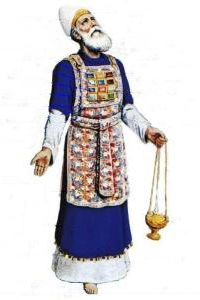
\includegraphics[width=50mm,scale=1.5]{Extras/Melchisedec.jpg}
\vspace{0.4in}  % Create a title for the document and write it in bold font
\LARGE{\textbf{\date}} % Again, do a line break
\linebreak 
% Create a subtitle \large{with Outlines, Statistics, Cross References, and Notes}
\vspace{0.5in}
\begin{flushleft}
\LARGE{Day \#48: Thursday, 17 February 2022  \\}\vspace{0.25in}
\LARGE{Numbers 22-24 Psalm 48 Proverb 17}
\end{flushleft}
\vspace{0.6in}
\bigskip

\normalsize{Xenia, Oh.\\}
\normalsize{created: \today}
\vspace{1.3in}

\end{flushright}
\end{titlepage}

\newpage 
\tableofcontents\hypertarget{TOC}{}
\listoffigures
\listoftables

\hyphenation{A-bim-e-lech bre-thren E-phra-im  Gib-e-o-nites Jer-u-sa-lem through-out Phil-i-stines The-o-phil-us Am-a-le-kites ven-geance Mesh-el-e-mi-ah onan-ism Phar-a-oh thoughts grev-ous-ness Hach-a-liah adul-ter-er Shad-rach}

%%%%%%%%%%%%%%%%% EXTRA COLORS
%%%%%%%%%%%%%%%%% EXTRA COLORS
%%%%%%%%%%%%%%%%% EXTRA COLORS
\definecolor{champagne}{rgb}{0.97,0.91,0.81}
\definecolor{bone}{rgb}{0.89,0.85,0.79}

\definecolor{ForestGreen}{rgb}{0.00,0.29,0.098}
\definecolor{GIVING}{cmyk}{1,0.0,0.72,.1}

\definecolor{MLPE}{cmyk}{1,1,0,.45}
\definecolor{SOCCER}{cmyk}{.77, 0, .42, .49}
\definecolor{PAYBILL}{cmyk}{0,0.83,0.76,0.07}
\definecolor{SERMON}{cmyk}{.14,.9,0,.30} % aka seance \href{http://www.flatuicolorpicker.com/purple-cmyk-color-model/}{seance}
\definecolor{BIBLE}{cmyk}{0,.17,.74,.17}
\definecolor{WORKBLUE}{cmyk}{1, .5, 0, .6}
\definecolor{myOrange}{cmyk}{0, .4, .98, .03}
\definecolor{myTan}{cmyk}{0.0,.07,.17,.10}
\definecolor{myRed}{cmyk}{0,1,1,0}
\definecolor{myWhite}{cmyk}{0,0,0,0}
\definecolor{BLUESoD}{cmyk}{.97,.84,0,.04}
\definecolor{WHITE}{cmyk}{0,0,0,0}
\definecolor{OLDGOLD}{cmyk}{0.05,0.3,1.00,0}
\definecolor{CASTLETON}{cmyk}{1,0,0.31,0.66}
\definecolor{cadmiumgreen}{rgb}{0.0, 0.42, 0.24}
\definecolor{jungle}{rgb}{0.203,0.4882,0.1718}
\definecolor{MYGOLD}{rgb}{1,.84,0}

\definecolor{MYLIGHTGRAY}{rgb}{.85,.85,.85}

\definecolor{codegreen}{rgb}{0,0.6,0}
\definecolor{codegray}{rgb}{0.5,0.5,0.5}
\definecolor{codepurple}{rgb}{0.58,0,0.82}
\definecolor{backcolour}{rgb}{0.95,0.95,0.92}


\mdfdefinestyle{MyFrame}{%
    linecolor=blue,
    outerlinewidth=2pt,
    roundcorner=5pt,
    innertopmargin=\baselineskip,
    innerbottommargin=\baselineskip,
    innerrightmargin=10pt,
    innerleftmargin=10pt,
    backgroundcolor=gray!25!white}


\mdfdefinestyle{MyFrame2}{%
    linecolor=black,
    outerlinewidth=2pt,
    roundcorner=5pt,
    innertopmargin=\baselineskip,
    innerbottommargin=\baselineskip,
    innerrightmargin=10pt,
    innerleftmargin=10pt,
    backgroundcolor=yellow!25!white}


%%%%%
%% for PFTTIS list
%%%%%

%%% And Joseph said unto
\index[PFTTIS]{And Joseph said unto!Genesis!Gen 40:008}
\index[PFTTIS]{And Joseph said unto!Genesis!Gen 40:012}
\index[PFTTIS]{And Joseph said unto!Genesis!Gen 41:025}
\index[PFTTIS]{And Joseph said unto!Genesis!Gen 42:014}
\index[PFTTIS]{And Joseph said unto!Genesis!Gen 42:018}
\index[PFTTIS]{And Joseph said unto!Genesis!Gen 44:015}
\index[PFTTIS]{And Joseph said unto!Genesis!Gen 45:003}
\index[PFTTIS]{And Joseph said unto!Genesis!Gen 45:004}
\index[PFTTIS]{And Joseph said unto!Genesis!Gen 46:031}
\index[PFTTIS]{And Joseph said unto!Genesis!Gen 48:009}
\index[PFTTIS]{And Joseph said unto!Genesis!Gen 48:018}
\index[PFTTIS]{And Joseph said unto!Genesis!Gen 50:019}
\index[PFTTIS]{And Joseph said unto!Genesis!Gen 50:024}


%%% a shadow
\index[PFTTIS]{a shadow!1Chronicles!1Chr 029:15}
\index[PFTTIS]{a shadow!Job!Job 008:09}
\index[PFTTIS]{a shadow!Job!Job 014:02}
\index[PFTTIS]{a shadow!Job!Job 017:07}
\index[PFTTIS]{a shadow!Psalm!Psa 102:011}
\index[PFTTIS]{a shadow!Psalm!Psa 144:004}
\index[PFTTIS]{a shadow!Ecclesiastes!Eccl 006:012}
\index[PFTTIS]{a shadow!Ecclesiastes!Eccl 008:013}
\index[PFTTIS]{a shadow!Isaiah!Isa 04:006}
\index[PFTTIS]{a shadow!Isaiah!Isa 25:004}
\index[PFTTIS]{a shadow!Jonah!Jnh 04:06}
\index[PFTTIS]{a shadow!Colossians!Col 02:017}
\index[PFTTIS]{a shadow!Hebews!Heb 10:001}

%%% blessed is the man
\index[PFTTIS]{blessed is the man!Psalm!Psa 001:001}
\index[PFTTIS]{blessed is the man!Psalm!Psa 032:002}
\index[PFTTIS]{blessed is the man!Psalm!Psa 034:008}
\index[PFTTIS]{blessed is the man!Psalm!Psa 065:004}
\index[PFTTIS]{blessed is the man!Psalm!Psa 084:005}
\index[PFTTIS]{blessed is the man!Psalm!Psa 084:012}
\index[PFTTIS]{blessed is the man!Psalm!Psa 094:012}
\index[PFTTIS]{blessed is the man!Psalm!Psa 112:001}
\index[PFTTIS]{blessed is the man!Proverbs!Pro 008:034}
\index[PFTTIS]{blessed is the man!Isaiah!Isa 056:002}
\index[PFTTIS]{blessed is the man!Jeremiah!Jer 017:007}
\index[PFTTIS]{blessed is the man!Romans!Rom 004:008}
\index[PFTTIS]{blessed is the man!James!Jam 001:012}


%%% carry them
\index[PFTTIS]{carry them!Leviticus!Lev 14:045}
\index[PFTTIS]{carry them!Numbers!Num 11:012}
\index[PFTTIS]{carry them!Joshua!Jsh 04:003}
\index[PFTTIS]{carry them!1Samuel!1Sam 20:040}
\index[PFTTIS]{carry them!1Kings!1Kng 08:046}
\index[PFTTIS]{carry them!2Chronicles!2Chr 06:036}
\index[PFTTIS]{carry them!Ezra!Ezra 05:015}
\index[PFTTIS]{carry them!Isaiah!Isa 40:011}
\index[PFTTIS]{carry them!Isaiah!Isa 41:016}
\index[PFTTIS]{carry them!Isaiah!Isa 57:013}
\index[PFTTIS]{carry them!Jeremiah!Jer 20:004}
\index[PFTTIS]{carry them!Jeremiah!Jer 20:005}
\index[PFTTIS]{carry them!Jeremiah!Jer 43:012}


\index[PFTTIS]{good tidings!2Samuel!2Sam 18:027}
\index[PFTTIS]{good tidings!1Kings!1Ki 01:042}
\index[PFTTIS]{good tidings!2Kings!2Ki 07:009 (2x)}
\index[PFTTIS]{good tidings!Isaiah!Isa 40:009 (2x)}
\index[PFTTIS]{good tidings!Isaiah!Isa 41:007}
\index[PFTTIS]{good tidings!Isaiah!Isa 52:007}
\index[PFTTIS]{good tidings!Isaiah!Isa 61:001}
\index[PFTTIS]{good tidings!Nahum!Nah 01:005}
\index[PFTTIS]{good tidings!Luke!Lk 02:010}
\index[PFTTIS]{good tidings!1Thessalonians!1Thess 03:006}


%%% dead body
\index[PFTTIS]{dead body!Leviticus!Lev 21:011}
\index[PFTTIS]{dead body!Numbers!Num 06:006}
\index[PFTTIS]{dead body!Numbers!Num 09:006}
\index[PFTTIS]{dead body!Numbers!Num 09:007}
\index[PFTTIS]{dead body!Numbers!Num 09:010}
\index[PFTTIS]{dead body!Numbers!Num 09:011}
\index[PFTTIS]{dead body!Numbers!Num 09:013}
\index[PFTTIS]{dead body!Numbers!Num 09:016}
\index[PFTTIS]{dead body!2Kings!2Ki 08:005}
\index[PFTTIS]{dead body!Isaiah!Isa 26:019}
\index[PFTTIS]{dead body!Jeremiah!Jer 26:023}
\index[PFTTIS]{dead body!Jeremiah!Jer 36:030}
\index[PFTTIS]{dead body!Haggai!Hag 02:013}

%%% great sea
\index[PFTTIS]{great sea!Numbers!Num 34:006}
\index[PFTTIS]{great sea!Numbers!Num 34:007}
\index[PFTTIS]{great sea!Joshua!Jos 01:004}
\index[PFTTIS]{great sea!Joshua!Jos 09:001}
\index[PFTTIS]{great sea!Joshua!Jos 15:012}
\index[PFTTIS]{great sea!Joshua!Jos 15:047}
\index[PFTTIS]{great sea!Joshua!Jos 23:004}
\index[PFTTIS]{great sea!Ezekiel!Eze 47:010}
\index[PFTTIS]{great sea!Ezekiel!Eze 47:015}
\index[PFTTIS]{great sea!Ezekiel!Eze 47:019}
\index[PFTTIS]{great sea!Ezekiel!Eze 47:020}
\index[PFTTIS]{great sea!Ezekiel!Eze 48:028}
\index[PFTTIS]{great sea!Daniel!Dan 07:002}


%%% have forsaken me
\index[PFTTIS]{have forsaken me!Judges!Jdg 10:013}
\index[PFTTIS]{have forsaken me!1Samuel!1Sam 08:008}
\index[PFTTIS]{have forsaken me!1Kings!1Ki 11:033}
\index[PFTTIS]{have forsaken me!2Kings!2Ki 22:017}
\index[PFTTIS]{have forsaken me!2Chronicles!2Chr 12:005}
\index[PFTTIS]{have forsaken me!2Chronicles!2Chr 34:025}
\index[PFTTIS]{have forsaken me!Jeremiah!Jer 01:016}
\index[PFTTIS]{have forsaken me!Jeremiah!Jer 02:013}
\index[PFTTIS]{have forsaken me!Jeremiah!Jer 05:007}
\index[PFTTIS]{have forsaken me!Jeremiah!Jer 05:019}
\index[PFTTIS]{have forsaken me!Jeremiah!Jer 16:011 (2x)}
\index[PFTTIS]{have forsaken me!Jeremiah!Jer 19:004}

%%% no king
\index[PFTTIS]{no king!Judges!Jdg 17:06}
\index[PFTTIS]{no king!Judges!Jdg 18:01}
\index[PFTTIS]{no king!Judges!Jdg 19:01}
\index[PFTTIS]{no king!Judges!Jdg 21:25}
\index[PFTTIS]{no king!1Kings!1Ki 22:47}
\index[PFTTIS]{no king!2Kings!2Ki 23:25}
\index[PFTTIS]{no king!Nehemiah!Neh 13:26}
\index[PFTTIS]{no king!Psalms!Psa 033:016}
\index[PFTTIS]{no king!Proverbs!Pro 30:27}
\index[PFTTIS]{no king!Daniel!Dan 02:10}
\index[PFTTIS]{no king!Hosea!Hos 10:03}
\index[PFTTIS]{no king!Micah!Mic 04:09}
\index[PFTTIS]{no king!John!Jhn 19:15}


%%% rebellious house
\index[PFTTIS]{rebellious house!Exodus!Exo 02:005}
\index[PFTTIS]{rebellious house!Exodus!Exo 02:006}
\index[PFTTIS]{rebellious house!Exodus!Exo 02:008}
\index[PFTTIS]{rebellious house!Exodus!Exo 03:009}
\index[PFTTIS]{rebellious house!Exodus!Exo 03:026}
\index[PFTTIS]{rebellious house!Exodus!Exo 03:027}
\index[PFTTIS]{rebellious house!Exodus!Exo 12:002 (2x)}
\index[PFTTIS]{rebellious house!Exodus!Exo 12:003}
\index[PFTTIS]{rebellious house!Exodus!Exo 12:009}
\index[PFTTIS]{rebellious house!Exodus!Exo 12:025}
\index[PFTTIS]{rebellious house!Exodus!Exo 17:012}
\index[PFTTIS]{rebellious house!Exodus!Exo 24:003}

%%% seek him
\index[PFTTIS]{seek him!Deuteronomy!Deu 04:029}\index[PFTTIS]{seek him!1Samuel!1Sam 23:025}
\index[PFTTIS]{seek him!1Chronicles!1Chr 28:009}
\index[PFTTIS]{seek him!2Chronicles!1Chr 15:002}
\index[PFTTIS]{seek him!Ezra!Ezr 08:022}
\index[PFTTIS]{seek him!Psalms!Psa 022:026}
\index[PFTTIS]{seek him!Psalms!Psa 024:006}
\index[PFTTIS]{seek him!Psalms!Psa 119:002}
\index[PFTTIS]{seek him!SoS!SoS 03:002}
\index[PFTTIS]{seek him!SoS!SoS 06:001}
\index[PFTTIS]{seek him!Hosea!Hos 07:010}
\index[PFTTIS]{seek him!Amos!Amo 05:008}
\index[PFTTIS]{seek him!Hebrews!Heb 11:0063}


%%% seek ye
\index[PFTTIS]{seek ye!Isaiah!Isa 34:016}
\index[PFTTIS]{seek ye!Isaiah!Isa 45:019}
\index[PFTTIS]{seek ye!Isaiah!Isa 55:006}
\index[PFTTIS]{seek ye!Amos!Amos 5:004}
\index[PFTTIS]{seek ye!John!John 1:38}
\index[PFTTIS]{seek ye!John!John 18:4}
\index[PFTTIS]{seek ye!John!John 18:7}
\index[PFTTIS]{seek ye!Matthew!Matt 6:33}
\index[PFTTIS]{seek ye!Numbers!Num 16:10}
\index[PFTTIS]{seek ye!Luke!Luke 12:31}
\index[PFTTIS]{seek ye!Luke!Luke 24:5}
\index[PFTTIS]{seek ye!Psalm!Psa 27:8}
\index[PFTTIS]{seek ye!Zephaniah!Zeph 2:3}

%%% the uncircumcised
\index[PFTTIS]{the uncircumcised!Genesis!Gen 17:014}
\index[PFTTIS]{the uncircumcised!Judges!Jdg 14:003}
\index[PFTTIS]{the uncircumcised!Judges!Jdg 15:018}
\index[PFTTIS]{the uncircumcised!2Samuel!2Sam 01:020}
\index[PFTTIS]{the uncircumcised!Isaiah!Isa 02:001}
\index[PFTTIS]{the uncircumcised!Jeremiah!Jer 09:025}
\index[PFTTIS]{the uncircumcised!Ezekiel!Eze 28:010}
\index[PFTTIS]{the uncircumcised!Ezekiel!Eze 31:018}
\index[PFTTIS]{the uncircumcised!Ezekiel!Eze 32:019}
\index[PFTTIS]{the uncircumcised!Ezekiel!Eze 32:027}
\index[PFTTIS]{the uncircumcised!Ezekiel!Eze 32:028}
\index[PFTTIS]{the uncircumcised!Ezekiel!Eze 32:029}
\index[PFTTIS]{the uncircumcised!Ezekiel!Eze 32:032}

%%% worship him
\index[PFTTIS]{worship him!Psalms!Psa 97:007}
\index[PFTTIS]{worship him!Zephaniah!Zeph 02:011}
\index[PFTTIS]{worship him!Matthew!Matt 02:002}
\index[PFTTIS]{worship him!Matthew!Matt 02:008}
\index[PFTTIS]{worship him!John!John 04:023}
\index[PFTTIS]{worship him!John!John 04:024 (2x)} 
\index[PFTTIS]{worship him!Acts!Acts 17:023}
\index[PFTTIS]{worship him!Hebrews!Heb 01:006}
\index[PFTTIS]{worship him!Revelation!Rev 04:010}
\index[PFTTIS]{worship him!Revelation!Rev 13:008}
\index[PFTTIS]{worship him!Revelation!Rev 14:007}
\index[PFTTIS]{worship him!Revelation!Rev 19:010}


%%%%%
%% for PFTTIS list
%%%%%

%%% afflictions
\index[WFTTIS]{afflictions!Psalms!Psa 34:019}
\index[WFTTIS]{afflictions!Psalms!Psa 132:001}
\index[WFTTIS]{afflictions!Acts!Acts 07:010}
\index[WFTTIS]{afflictions!Acts!Acts 20:023}
\index[WFTTIS]{afflictions!2Corinthians!2Cor 06:004}
\index[WFTTIS]{afflictions!Colossians!Col 01:024}
\index[WFTTIS]{afflictions!1Thessalonians!1Thess 03:003}
\index[WFTTIS]{afflictions!2Timothy!2Tim 01:008}
\index[WFTTIS]{afflictions!2Timothy!2Tim 03:011}
\index[WFTTIS]{afflictions!2Timothy!2Tim 04:005}
\index[WFTTIS]{afflictions!Hebrews!Heb 10:032}
\index[WFTTIS]{afflictions!Hebrews!Heb 10:033}
\index[WFTTIS]{afflictions!1Peter!1Pet 05:009}

%%% acsend
\index[WFTTIS]{acsend!Joshua!Jos 06:05}
\index[WFTTIS]{acsend!Psalm!Psa 024:003}
\index[WFTTIS]{acsend!Psalm!Psa 135:007}
\index[WFTTIS]{acsend!Psalm!Psa 139:008}
\index[WFTTIS]{acsend!Isaiah!Isa 14:013}
\index[WFTTIS]{acsend!Isaiah!Isa 14:014}
\index[WFTTIS]{acsend!Jeremiah!Jer 10:013}
\index[WFTTIS]{acsend!Jeremiah!Jer 51:016}
\index[WFTTIS]{acsend!Ezekiel!Eze 38:009}
\index[WFTTIS]{acsend!John!John 06:062}
\index[WFTTIS]{acsend!John!John 20:017}
\index[WFTTIS]{acsend!Romans!Rom 10:006}
\index[WFTTIS]{acsend!Revelation!Rev 17:008}

%%% Assyrian
\index[WFTTIS]{Assyrian!Isaiah!Isa 10:005}
\index[WFTTIS]{Assyrian!Isaiah!Isa 10:024}
\index[WFTTIS]{Assyrian!Isaiah!Isa 14:025}
\index[WFTTIS]{Assyrian!Isaiah!Isa 19:023}
\index[WFTTIS]{Assyrian!Isaiah!Isa 23:013}
\index[WFTTIS]{Assyrian!Isaiah!Isa 30:031}
\index[WFTTIS]{Assyrian!Isaiah!Isa 31:008}
\index[WFTTIS]{Assyrian!Isaiah!Isa 52:004}
\index[WFTTIS]{Assyrian!Ezekiel!Eze 31:003}
\index[WFTTIS]{Assyrian!Hosea!Hos 05:013}
\index[WFTTIS]{Assyrian!Hosea!Hos 11:005}
\index[WFTTIS]{Assyrian!Micah!Hos 05:005}
\index[WFTTIS]{Assyrian!Micah!Hos 05:006}

%%% blot
\index[WFTTIS]{blot!Exodus!Exo 32:032}
\index[WFTTIS]{blot!Exodus!Exo 32:033}
\index[WFTTIS]{blot!Numbers!Num 05:026}
\index[WFTTIS]{blot!Deuteronomy!Deut 09:014}
\index[WFTTIS]{blot!Deuteronomy!Deut 25:019}
\index[WFTTIS]{blot!Deuteronomy!Deut 29:020}
\index[WFTTIS]{blot!2Kings!2Ki 14:027}
\index[WFTTIS]{blot!Job!Job 31:007}
\index[WFTTIS]{blot!Psalms!Psa 51:001}
\index[WFTTIS]{blot!Psalms!Psa 51:009}
\index[WFTTIS]{blot!Proverbs!Pro 09:007}
\index[WFTTIS]{blot!Jeremiah!Jer 18:023}
\index[WFTTIS]{blot!Revelation!Rev 03:005}


%%% chain
\index[WFTTIS]{chain!Genesis!Gen 41:042}
\index[WFTTIS]{chain!1Kings!1Ki 07:017}
\index[WFTTIS]{chain!Psalms!Psa 73:006}
\index[WFTTIS]{chain!SoS!Sos 04:009}
\index[WFTTIS]{chain!Lamentations!Lam 03:007}
\index[WFTTIS]{chain!Ezekiel!Eze 07:023}
\index[WFTTIS]{chain!Ezekiel!Eze 16:011}
\index[WFTTIS]{chain!Daniel!Dan 05:007}
\index[WFTTIS]{chain!Daniel!Dan 05:016}
\index[WFTTIS]{chain!Daniel!Dan 05:029}
\index[WFTTIS]{chain!Acts!Acts 28:020}
\index[WFTTIS]{chain!2Timothy!2Tim 01:016}
\index[WFTTIS]{chain!Revelation!Rev 20:001}


%%% controversy
\index[WFTTIS]{controversy!Deuteronomy!Deu 17:008}
\index[WFTTIS]{controversy!Deuteronomy!Deu 19:017}
\index[WFTTIS]{controversy!Deuteronomy!Deu 21:005}
\index[WFTTIS]{controversy!Deuteronomy!Deu 25:001}
\index[WFTTIS]{controversy!2Samuel!2Sam 15:002}
\index[WFTTIS]{controversy!Isaiah!Isa 34:008}
\index[WFTTIS]{controversy!Jeremiah!Jer 25:031}
\index[WFTTIS]{controversy!Ezekiel!Eze 44:024}
\index[WFTTIS]{controversy!Hosea!Hos 04:001}
\index[WFTTIS]{controversy!Hosea!Hos 12:002}
\index[WFTTIS]{controversy!Micah!Mic 06:002 (2x)}
\index[WFTTIS]{controversy!1Timothy!1Tim 03:016}


%%% Dagon/Dagon's
\index[WFTTIS]{Dagon!Judges!Jdg 16:023}
\index[WFTTIS]{Dagon!1Samuel!1Sam 05:002 (2x)}
\index[WFTTIS]{Dagon!1Samuel!1Sam 05:003 (2x)}
\index[WFTTIS]{Dagon!1Samuel!1Sam 05:004 (3x)}
\index[WFTTIS]{Dagon!1Samuel!1Sam 05:005 (3x)}
\index[WFTTIS]{Dagon!1Samuel!1Sam 05:007}
\index[WFTTIS]{Dagon!1Chronicles!1Chr 10:010}

%%% disobedient
\index[WFTTIS]{disobedient!1Kings!1Ki 13:026}
\index[WFTTIS]{disobedient!Nehemiah!Neh 09:026}
\index[WFTTIS]{disobedient!Luke!Luke 01:017}
\index[WFTTIS]{disobedient!Acts!Acts 26:019}
\index[WFTTIS]{disobedient!Romans!Rom 01:030}
\index[WFTTIS]{disobedient!Romans!Rom 10:021}
\index[WFTTIS]{disobedient!1Timothy!1Tim 01:009}
\index[WFTTIS]{disobedient!2Timothy!2Tim 03:002}
\index[WFTTIS]{disobedient!Titus!Titus 01:016}
\index[WFTTIS]{disobedient!Titus!Titus 03:003}
\index[WFTTIS]{disobedient!1Peter!1Pet 02:007}
\index[WFTTIS]{disobedient!1Peter!1Pet 02:008}
\index[WFTTIS]{disobedient!1Peter!1Pet 03:020}


%%% doubt
\index[WFTTIS]{doubt!Genesis!Gen 37:033}
\index[WFTTIS]{doubt!Deuteronomy!Deu 28:066}
\index[WFTTIS]{doubt!Job!Job 12:002}
\index[WFTTIS]{doubt!Matthew!Matt 14:031}
\index[WFTTIS]{doubt!Matthew!Matt 21:021}
\index[WFTTIS]{doubt!Mark!Mk 11:023}
\index[WFTTIS]{doubt!Luke!Lk 11:020}
\index[WFTTIS]{doubt!John!Jhn 10:024}
\index[WFTTIS]{doubt!Acts!Acts 02:012}
\index[WFTTIS]{doubt!Acts!Acts 28:004}
\index[WFTTIS]{doubt!1Corinthians!1Cor 09:010}
\index[WFTTIS]{doubt!Galatians!Gal 04:020}
\index[WFTTIS]{doubt!1John!1Jhn 02:019}


%%% dungeon
\index[WFTTIS]{dungeon!Genesis!Gen 40:015}
\index[WFTTIS]{dungeon!Genesis!Gen 41:014}
\index[WFTTIS]{dungeon!Exodus!Exo 12:029}
\index[WFTTIS]{dungeon!Jeremiah!Jer 37:016}
\index[WFTTIS]{dungeon!Jeremiah!Jer 38:006 (2x)}
\index[WFTTIS]{dungeon!Jeremiah!Jer 38:007}
\index[WFTTIS]{dungeon!Jeremiah!Jer 38:009}
\index[WFTTIS]{dungeon!Jeremiah!Jer 38:010}
\index[WFTTIS]{dungeon!Jeremiah!Jer 38:011}
\index[WFTTIS]{dungeon!Jeremiah!Jer 38:013}
\index[WFTTIS]{dungeon!Lamentations!Lam 03:053}
\index[WFTTIS]{dungeon!Lamentations!Lam 03:055}


%%% error
\index[WFTTIS]{error!2Samuel!2Sam 06:007}
\index[WFTTIS]{error!Job!Job 19:004}
\index[WFTTIS]{error!Ecclesiastes!Ecc 05:006}
\index[WFTTIS]{error!Ecclesiastes!Ecc 10:005}
\index[WFTTIS]{error!Isaiah!Isa 32:006}
\index[WFTTIS]{error!Daniel!Dan 06:004}
\index[WFTTIS]{error!Matthew!Matt 27:064}
\index[WFTTIS]{error!Romans!Rom 01:027}
\index[WFTTIS]{error!James!Jam 05:020}
\index[WFTTIS]{error!2Peter!2Pet 02:018}
\index[WFTTIS]{error!2Peter!2Pet 03:017}
\index[WFTTIS]{error!1John!1Jn 04:006}
\index[WFTTIS]{error!Jude!Jude 01:011}

%%% fourish
\index[WFTTIS]{fourish!Psalms!Psa 072:007}
\index[WFTTIS]{fourish!Psalms!Psa 072:016}
\index[WFTTIS]{fourish!Psalms!Psa 092:007}
\index[WFTTIS]{fourish!Psalms!Psa 092:012}
\index[WFTTIS]{fourish!Psalms!Psa 092:013}
\index[WFTTIS]{fourish!Psalms!Psa 132:018}
\index[WFTTIS]{fourish!Proverbs!Pro 11:28}
\index[WFTTIS]{fourish!Proverbs!Pro 14:11}
\index[WFTTIS]{fourish!Ecclesiastes!Ecc 12:05}
\index[WFTTIS]{fourish!SongOfSolomon!SOS 07:12}
\index[WFTTIS]{fourish!Isaiah!Isa 17:11}
\index[WFTTIS]{fourish!Isaiah!Isa 66:14}
\index[WFTTIS]{fourish!Ezekiel!Eze 17:24}




%%% giants
\index[WFTTIS]{giants!Genesis!Gen 06:004}
\index[WFTTIS]{giants!Numbers!Num 13:033}
\index[WFTTIS]{giants!Deuteronomy!Deut 02:011}
\index[WFTTIS]{giants!Deuteronomy!Deut 02:021}
\index[WFTTIS]{giants!Deuteronomy!Deut 03:011}
\index[WFTTIS]{giants!Deuteronomy!Deut 03:013}
\index[WFTTIS]{giants!Joshua!Josh 12:004}
\index[WFTTIS]{giants!Joshua!Josh 13:012}
\index[WFTTIS]{giants!Joshua!Josh 15:008}
\index[WFTTIS]{giants!Joshua!Josh 17:015}
\index[WFTTIS]{giants!Joshua!Josh 16:016}

%%% good man
\index[WFTTIS]{good man!2 Samuel!2Sa 18:27}
%(1) Psalms 37:23 [5]
%(1) Psalms 112:5 [2]
%(1) Proverbs 12:2 [2]
%(1) Proverbs 13:22 [2]
%(1) Proverbs 14:14 [14]
%(1) Micah 7:2 [2]
%(1) Matthew 12:35 [2]
%(1) Luke 6:45 [2]
%(1) Luke 23:50 [15]
%(1) John 7:12 [17]
%(1) Acts 11:24 [5]
%(1) Romans 5:7 [14]

%%% Hinnom
\index[WFTTIS]{Hinnom!Joshua!Jsh 15:008}
\index[WFTTIS]{Hinnom!Joshua!Jsh 18:016}
\index[WFTTIS]{Hinnom!2Kings!2Ki 23:010}
\index[WFTTIS]{Hinnom!2Chronicles!2Chr 28:003}
\index[WFTTIS]{Hinnom!2Chronicles!2Chr 33:006}
\index[WFTTIS]{Hinnom!Nehemiah!Neh 11:030}
\index[WFTTIS]{Hinnom!Jeremiah!Jer 07:031}
\index[WFTTIS]{Hinnom!Jeremiah!Jer 07:032}
\index[WFTTIS]{Hinnom!Jeremiah!Jer 19:002}
\index[WFTTIS]{Hinnom!Jeremiah!Jer 19:006}
\index[WFTTIS]{Hinnom!Jeremiah!Jer 32:035}

%%% inclined
\index[WFTTIS]{inclined!Judges!Jdg 09:003}
\index[WFTTIS]{inclined!Psalms!Psa 040:001}
\index[WFTTIS]{inclined!Psalms!Psa 116:002}
\index[WFTTIS]{inclined!Psalms!Psa 119:112}
\index[WFTTIS]{inclined!Proverbs!Pro 05:13}
\index[WFTTIS]{inclined!Jeremiah!Jer 07:24}
\index[WFTTIS]{inclined!Jeremiah!Jer 07:26}
\index[WFTTIS]{inclined!Jeremiah!Jer 11:08}
\index[WFTTIS]{inclined!Jeremiah!Jer 17:23}
\index[WFTTIS]{inclined!Jeremiah!Jer 25:04}
\index[WFTTIS]{inclined!Jeremiah!Jer 34:14}
\index[WFTTIS]{inclined!Jeremiah!Jer 35:15}
\index[WFTTIS]{inclined!Jeremiah!Jer 44:05}


%%% laughed
\index[WFTTIS]{laughed!Genesis!Gen 17:017}
\index[WFTTIS]{laughed!Genesis!Gen 18:012}
\index[WFTTIS]{laughed!Genesis!Gen 18:015}
\index[WFTTIS]{laughed!2Kings!2Ki 19:021}
\index[WFTTIS]{laughed!2Chronicles!2Chr 30:010}
\index[WFTTIS]{laughed!Nehemiah!Neh 02:019}
\index[WFTTIS]{laughed!Job!Job 12:004}
\index[WFTTIS]{laughed!Job!Job 29:024}
\index[WFTTIS]{laughed!Isaiah!Isa 37:022}
\index[WFTTIS]{laughed!Ezekiel!Ezek 23:032}
\index[WFTTIS]{laughed!Matthew!Matt 09:024}
\index[WFTTIS]{laughed!Mark!Mk 05:040}
\index[WFTTIS]{laughed!Luke!Lk 08:053}

%%% liar
\index[WFTTIS]{liar!Job!Job 24:025}
\index[WFTTIS]{liar!Proverbs!Pro 17:004}
\index[WFTTIS]{liar!Proverbs!Pro 19:022}
\index[WFTTIS]{liar!Proverbs!Pro 30:006}
\index[WFTTIS]{liar!Jeremiah!Jer 15:018}
\index[WFTTIS]{liar!John!Jhn 08:044}
\index[WFTTIS]{liar!John!Jhn 08:055}
\index[WFTTIS]{liar!Romans!Rom 03:004}
\index[WFTTIS]{liar!1John!1Jhn 01:010}
\index[WFTTIS]{liar!1John!1Jhn 02:004}
\index[WFTTIS]{liar!1John!1Jhn 02:022}
\index[WFTTIS]{liar!1John!1Jhn 04:020}
\index[WFTTIS]{liar!1John!1Jhn 05:010}

%%% palsy
\index[WFTTIS]{palsy!Matthew!Matt 04:024}
\index[WFTTIS]{palsy!Matthew!Matt 08:006}
\index[WFTTIS]{palsy!Matthew!Matt 09:002}
\index[WFTTIS]{palsy!Matthew!Matt 09:006}
\index[WFTTIS]{palsy!Mark!Mk 02:003}
\index[WFTTIS]{palsy!Mark!Mk 02:004}
\index[WFTTIS]{palsy!Mark!Mk 02:005}
\index[WFTTIS]{palsy!Mark!Mk 02:009}
\index[WFTTIS]{palsy!Mark!Mk 02:010}
\index[WFTTIS]{palsy!Luke!Lk 05:018}
\index[WFTTIS]{palsy!Luke!Lk 05:024}
\index[WFTTIS]{palsy!Acts!Acts 09:033}

%%% Profitable
\index[WFTTIS]{profitable!Job!Job 22:002 (2x)}
\index[WFTTIS]{profitable!Ecclesiastes!Ecc 10:010}
\index[WFTTIS]{profitable!Isaiah!Isa 44:010}
\index[WFTTIS]{profitable!Jeremiah!Jer 13:007}
\index[WFTTIS]{profitable!Matthew!Matt 05:029}
\index[WFTTIS]{profitable!Matthew!Matt 05:030}
\index[WFTTIS]{profitable!Acts!Acts 20:020}
\index[WFTTIS]{profitable!1Timothy!1Tim 04:008}
\index[WFTTIS]{profitable!2Timothy!2Tim 03:016}
\index[WFTTIS]{profitable!2Timothy!2Tim 04:011}
\index[WFTTIS]{profitable!Titus!Titus 03:008}
\index[WFTTIS]{profitable!Philemon!Phlm 01:011}

%%% Rechab
\index[WFTTIS]{Rechab!2Samuel!2Sam 04:002}
\index[WFTTIS]{Rechab!2Samuel!2Sam 04:005}
\index[WFTTIS]{Rechab!2Samuel!2Sam 04:006}
\index[WFTTIS]{Rechab!2Samuel!2Sam 04:009}
\index[WFTTIS]{Rechab!2KIngs!2Ki 10:015}
\index[WFTTIS]{Rechab!2KIngs!2Ki 10:023}
\index[WFTTIS]{Rechab!1Chronicles!1Chr 02:055}
\index[WFTTIS]{Rechab!Nehemiah!Neh 03:014}
\index[WFTTIS]{Rechab!Jeremiah!Jer 35:006}
\index[WFTTIS]{Rechab!Jeremiah!Jer 35:008}
\index[WFTTIS]{Rechab!Jeremiah!Jer 35:014}
\index[WFTTIS]{Rechab!Jeremiah!Jer 35:016}
\index[WFTTIS]{Rechab!Jeremiah!Jer 35:019}

%%% serpents
\index[WFTTIS]{serpents!Exodus!Exo 07:012}
\index[WFTTIS]{serpents!Numbers!Num 21:006}
\index[WFTTIS]{serpents!Numbers!Num 21:007}
\index[WFTTIS]{serpents!Deuteronomy!Deu 08:015}
\index[WFTTIS]{serpents!Deuteronomy!Deu 32:024}
\index[WFTTIS]{serpents!Jeremiah!Jer 08:017}
\index[WFTTIS]{serpents!Matthew!Matt 10:016}
\index[WFTTIS]{serpents!Matthew!Matt 23:033}
\index[WFTTIS]{serpents!Mark!Mk 16:018}
\index[WFTTIS]{serpents!Luke!Lk 10:019}
\index[WFTTIS]{serpents!1Corinthians!1Cor 10:009}
\index[WFTTIS]{serpents!James!Jas 03:007}
\index[WFTTIS]{serpents!Revelation!Rev 09:019}

%%% short
\index[WFTTIS]{short!Numbers!Num 11:023}
\index[WFTTIS]{short!2Kings!2Ki 10:032}
\index[WFTTIS]{short!Job!Job 17:012}
\index[WFTTIS]{short!Job!Job 20:005}
\index[WFTTIS]{short!Psalms!Psa 89:047}
\index[WFTTIS]{short!Romans!Rom 03:023}
\index[WFTTIS]{short!Romans!Rom 09:028  (2x)}
\index[WFTTIS]{short!1Corinthians!1Cor 07:029}
\index[WFTTIS]{short!1Thessalonians!1Thess 02:017}
\index[WFTTIS]{short!Hebrews!Heb 04:001}
\index[WFTTIS]{short!Revelation!Rev 12:012}
\index[WFTTIS]{short!Revelation!Rev 17:010}

%%% smiteth
\index[WFTTIS]{smiteth!Exodus!Exo 21:012}
\index[WFTTIS]{smiteth!Exodus!Exo 21:15}
\index[WFTTIS]{smiteth!Deuteronomy!Dt 25:11}
\index[WFTTIS]{smiteth!Deuteronomy!Dt 27:24}
\index[WFTTIS]{smiteth!Joshua!Jsh 15:16}
\index[WFTTIS]{smiteth!Judges!Jdg 15:16}
\index[WFTTIS]{smiteth!2 Samuel!2Sa 05:08}
\index[WFTTIS]{smiteth!1Chronicles!1Chr 11:06}
\index[WFTTIS]{smiteth!Job!1Chr 26:12}
\index[WFTTIS]{smiteth!Isaiah!Isa 09:13}
\index[WFTTIS]{smiteth!Lamentations!Lam 03:30}
\index[WFTTIS]{smiteth!Ezekiel!Eze 07:09}
\index[WFTTIS]{smiteth!Luke!Lk 06:29}



%%% vanities
\index[WFTTIS]{vanities!Deuteronomy!Deut 21:021}
\index[WFTTIS]{vanities!1Kings!1Ki 16:013}
\index[WFTTIS]{vanities!1Kings!1Ki 16:026}
\index[WFTTIS]{vanities!Psalms!Psa 031:006}
\index[WFTTIS]{vanities!Ecclesiastes!Ecc 01:002 (2x)}
\index[WFTTIS]{vanities!Ecclesiastes!Ecc 05:007}
\index[WFTTIS]{vanities!Ecclesiastes!Ecc 12:008}
\index[WFTTIS]{vanities!Jeremiah!Jer 08:019}
\index[WFTTIS]{vanities!Jeremiah!Jer 10:008}
\index[WFTTIS]{vanities!Jeremiah!Jer 14:022}
\index[WFTTIS]{vanities!Jonah!Jnh 02:008}
\index[WFTTIS]{vanities!Acts!Acts 14:015}



%%%%%
%% for PFTTIS list
%%%%%

%%% worm
\index[WFITV]{worm!Exodus!Exo 16:024}
\index[WFITV]{worm!Job!Job 17:014}
\index[WFITV]{worm!Job!Job 24:029}
\index[WFITV]{worm!Job!Job 25:005 (2x)}
\index[WFITV]{worm!Psalms!Psa 022:006}
\index[WFITV]{worm!Isaiah!Isa 14:011}
\index[WFITV]{worm!Isaiah!Isa 41:014}
\index[WFITV]{worm!Isaiah!Isa 51:008}
\index[WFITV]{worm!Isaiah!Isa 66:024}
\index[WFITV]{worm!Jonah!Jnh 04:007}
\index[WFITV]{worm!Mark!Mk 09:044}
\index[WFITV]{worm!Mark!Mk 09:046}
\index[WFITV]{worm!Mark!Mk 09:048}


%\subsubsection{Title}
%\textbf{Introduction:} Isaiah 46 
%\index[speaker]{Speaker!Isaiah 49 (Title}
%\index[series]{Book (Speaker)!IPassage (Title)}
%\index[date]{2017/07/09!Isaiah 49 (Title)}
%\begin{compactenum}[I.]
%    \item  \textbf{Point} \index[scripture]{Isaiah!IPassage} (IPassage)
%\end{compactenum}




  


%\input{02OT-Exodus/ExodusIntroduction}
\newpage
\begin{figure}
\begin{center}
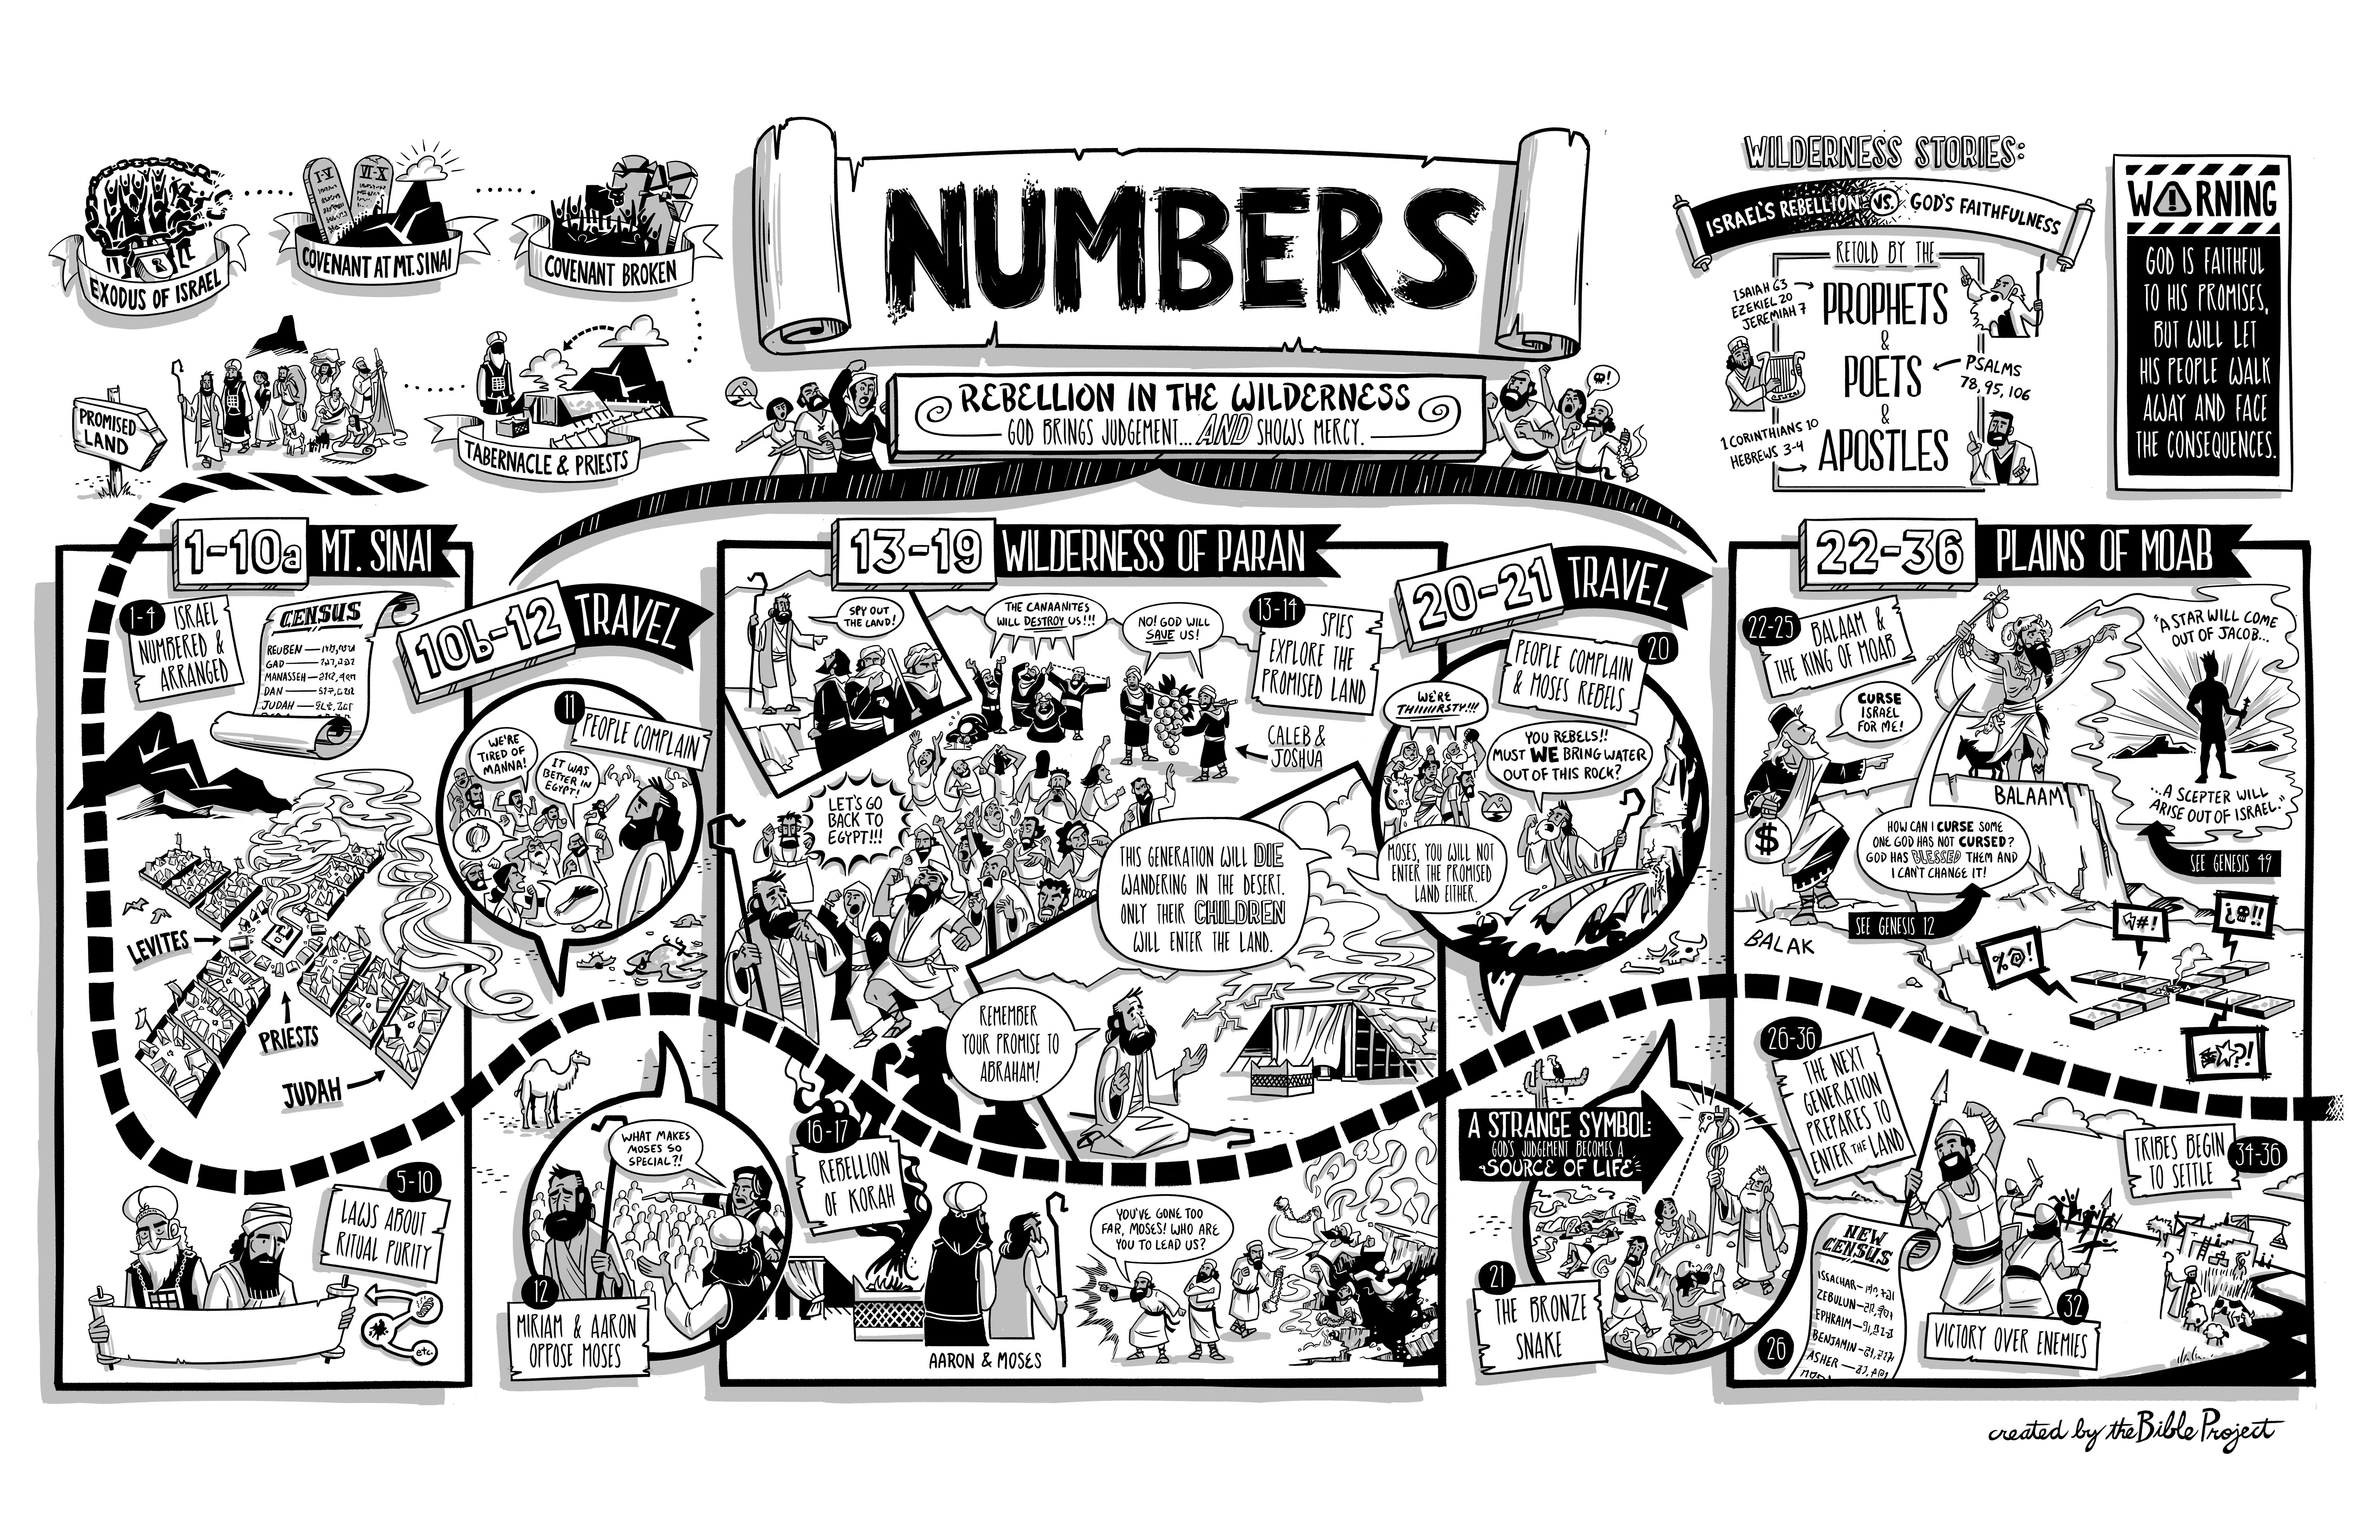
\includegraphics[scale=0.5, angle=90]{04OT-Numbers/References/BibleProject-Numbers.jpg}
\caption[Numbers from the Bible Project]{Numbers from the Bible Project}
\label{fig:Numbers from the Bible Project}
\end{center}
\end{figure}

\newpage
\begin{figure}
\begin{center}
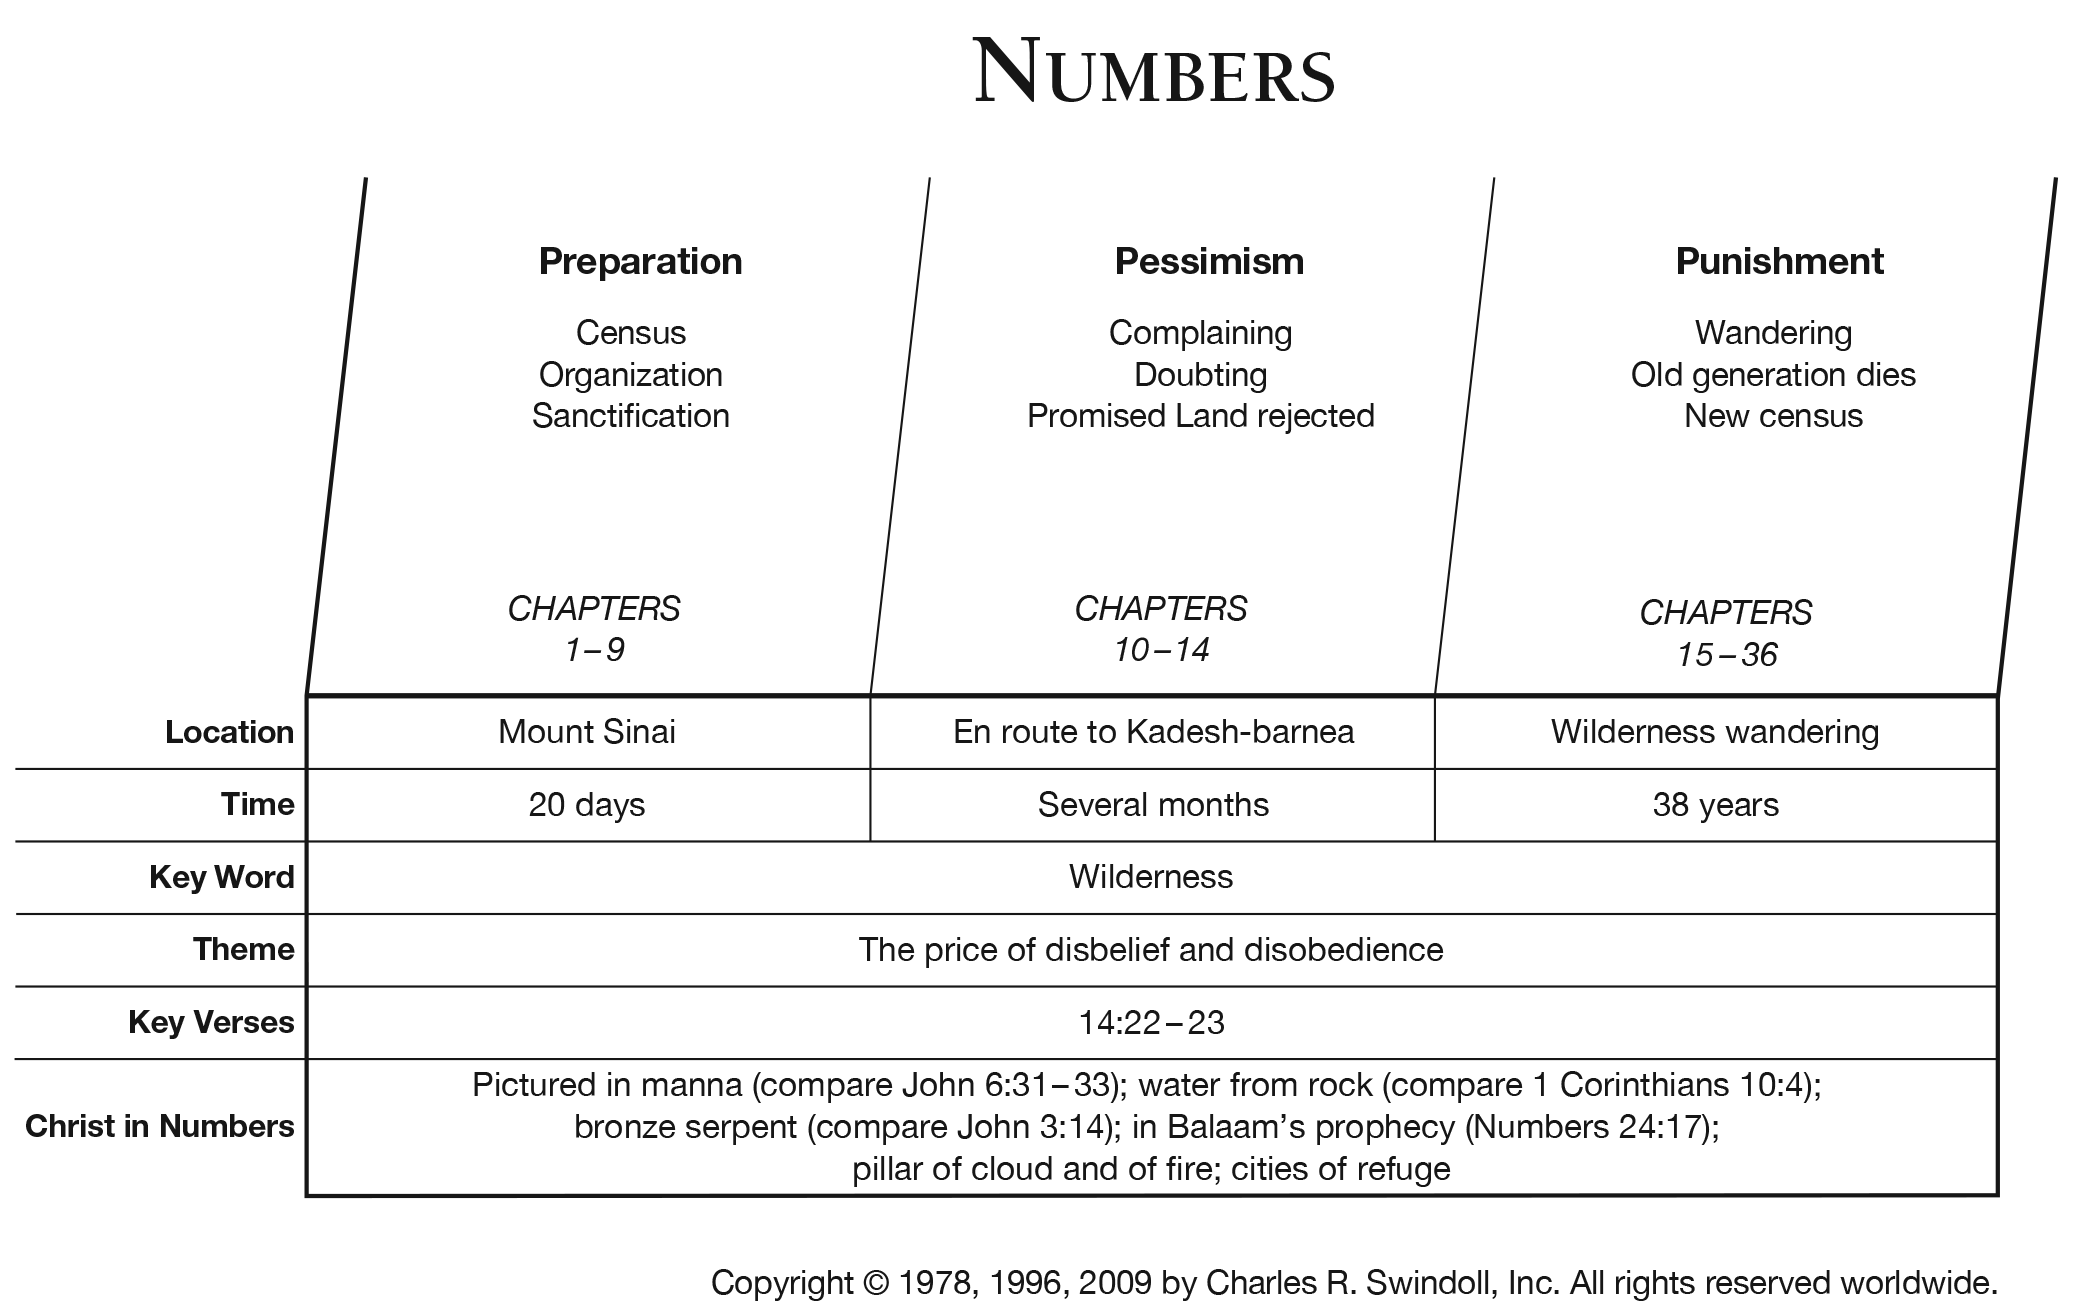
\includegraphics[scale=0.3, angle=90]{04OT-Numbers/References/Swindoll-Numbers.png}
\caption[Numbers by Swindoll]{Numbers by Swindoll}
\label{fig:Numbers by Swindoll}
\end{center}
\end{figure}

\newpage
\begin{figure}
\begin{center}
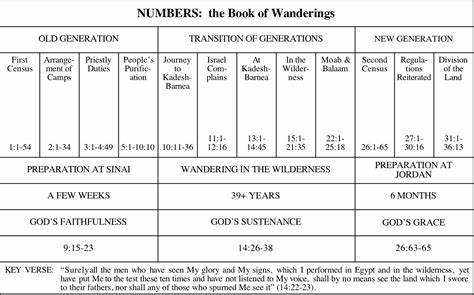
\includegraphics[scale=1.2, angle=90]{04OT-Numbers/References/Numbers.jpg}
\caption[Numbers by Unknown]{Numbers by Unknown}
\label{fig:Numbers by Unknown}
\end{center}
\end{figure}

\newpage
\begin{figure}
\begin{center}
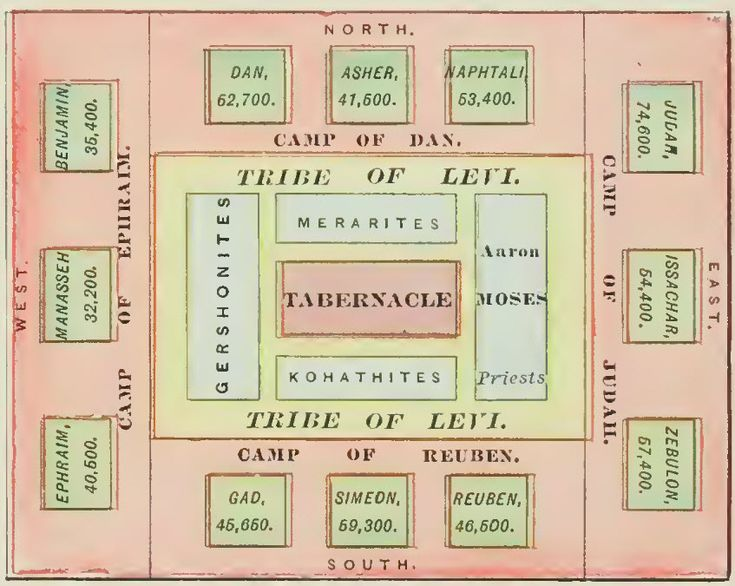
\includegraphics[scale=.8, angle=0]{04OT-Numbers/References/LayoutOfTribesAndTabernacle.jpg}
\caption[Layout of Tribes and Tabernacle]{Layout of Tribes and Tabernacle}
\label{fig:Layout of Tribes and Tabernacle}
\end{center}
\end{figure}


\chapter{Numbers 22}

\begin{figure}
  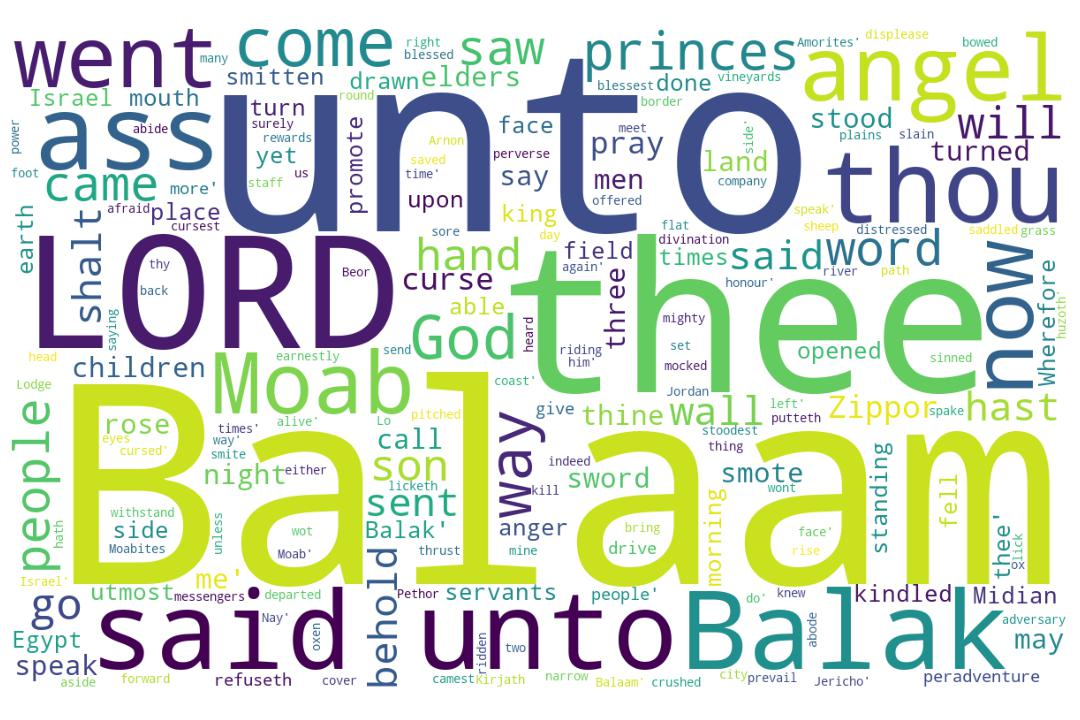
\includegraphics[width=\linewidth]{04OT-Numbers/Numbers22-WordCloud.jpg}
  \caption{Numbers 22 Word Cloud}
  \label{fig:Numbers 22 word Cloud}
\end{figure}

\marginpar{\scriptsize \centering \fcolorbox{bone}{lime}{\textbf{BALAAM'S RELIGION }}\\ (Numbers 22) \begin{compactenum}[I.][8]
    \item  \textbf{Assigned Diplomats} \index[scripture]{Numbers!Num 22:05}\index[scripture]{Numbers!Num 22:15} (Numbers 22:5, 15)
    \item  \textbf{Asking for Divination} \index[scripture]{Numbers!Num 22:07} (Numbers 22:7)
    \item Balaam's \textbf{Attempted Disobedience} \index[scripture]{Numbers!Num 22:19} (Numbers 22:19)
    \item \textbf{Armament Drawn} \index[scripture]{Numbers!Num 22:23}\index[scripture]{Numbers!Num 22:31} (Numbers 22:23, 31)
    \item The \textbf{Ass falls Down} \index[scripture]{Numbers!Num 22:27} (Numbers 22:27)
    \item An \textbf{Argument with a Donkey} \index[scripture]{Numbers!Num 22:29} (Numbers 22:29)
    \item An \textbf{Acquired Doctrine} \index[scripture]{Numbers!Num 23}\index[scripture]{Revelation!Rev 02:14} (Numbers 22, Revelation 2:14)
\end{compactenum}}

%%%%%%%%%%%%%%%%%%%%%%%%%%%%%%%%%%%%%
%%%%%%%%%%%%%%%%%%%%%%%%%%%%%%%%%%%%%
\footnote{\textcolor[rgb]{0.00,0.25,0.00}{\hyperlink{NumbersTOC}{Return to end of Table of Contents.}}}\footnote{\href{https://audiobible.com/bible/numbers_22.html}{\textcolor[cmyk]{0.99998,1,0,0}{Numbers 22 Audio}}}\textcolor[cmyk]{0.99998,1,0,0}{And the children of Israel set forward, and pitched in the plains of Moab on this side Jordan \emph{by} Jericho.}\\
\\
\P \textcolor[cmyk]{0.99998,1,0,0}{And Balak the son of Zippor saw all that Israel had done to the Amorites.}
[3] \textcolor[cmyk]{0.99998,1,0,0}{And Moab was sore afraid of the people, because they \emph{were} many: and Moab was distressed because of the children of Israel.}
[4] \textcolor[cmyk]{0.99998,1,0,0}{And Moab said unto the elders of Midian, Now shall this company lick up all \emph{that} \emph{are} round about us, as the ox licketh up the grass of the field. And Balak the son of Zippor \emph{was} king of the Moabites at that time.}
[5] \textcolor[cmyk]{0.99998,1,0,0}{He sent messengers therefore unto Balaam the son of Beor to Pethor, which \emph{is} by the river of the land of the children of his people, to call him, saying, Behold, there is a people come out from Egypt: behold, they cover the face of the earth, and they abide over against me:}
[6] \textcolor[cmyk]{0.99998,1,0,0}{Come now therefore, I pray thee, curse me this people; for they \emph{are} too mighty for me: peradventure I shall prevail, \emph{that} we may smite them, and \emph{that} I may drive them out of the land: for I wot that he whom thou blessest \emph{is} blessed, and he whom thou cursest is cursed.}
[7] \textcolor[cmyk]{0.99998,1,0,0}{And the elders of Moab and the elders of Midian departed with the rewards of divination in their hand; and they came unto Balaam, and spake unto him the words of Balak.}
[8] \textcolor[cmyk]{0.99998,1,0,0}{And he said unto them, Lodge here this night, and I will bring you word again, as the LORD shall speak unto me: and the princes of Moab abode with Balaam.}
[9] \textcolor[cmyk]{0.99998,1,0,0}{And God came unto Balaam, and said, What men \emph{are} these with thee?}
[10] \textcolor[cmyk]{0.99998,1,0,0}{And Balaam said unto God, Balak the son of Zippor, king of Moab, hath sent unto me, \emph{saying},}
[11] \textcolor[cmyk]{0.99998,1,0,0}{Behold, \emph{there} \emph{is} a people come out of Egypt, which covereth the face of the earth: come now, curse me them; peradventure I shall be able to overcome them, and drive them out.}
[12] \textcolor[cmyk]{0.99998,1,0,0}{And God said unto Balaam, Thou shalt not go with them; thou shalt not curse the people: for they \emph{are} blessed.}
[13] \textcolor[cmyk]{0.99998,1,0,0}{And Balaam rose up in the morning, and said unto the princes of Balak, Get you into your land: for the LORD refuseth to give me leave to go with you.}
[14] \textcolor[cmyk]{0.99998,1,0,0}{And the princes of Moab rose up, and they went unto Balak, and said, Balaam refuseth to come with us.}\\
\\
\P \textcolor[cmyk]{0.99998,1,0,0}{And Balak sent yet again princes, more, and more honourable than they.}
[16] \textcolor[cmyk]{0.99998,1,0,0}{And they came to Balaam, and said to him, Thus saith Balak the son of Zippor, Let nothing, I pray thee, hinder thee from coming unto me:}
[17] \textcolor[cmyk]{0.99998,1,0,0}{For I will promote thee unto very great honour, and I will do whatsoever thou sayest unto me: come therefore, I pray thee, curse me this people.}
[18] \textcolor[cmyk]{0.99998,1,0,0}{And Balaam answered and said unto the servants of Balak, If Balak would give me his house full of silver and gold, I cannot go beyond the word of the LORD my God, to do less or more.}
[19] \textcolor[cmyk]{0.99998,1,0,0}{Now therefore, I pray you, tarry ye also here this night, that I may know what the LORD will say unto me more.}
[20] \textcolor[cmyk]{0.99998,1,0,0}{And God came unto Balaam at night, and said unto him, If the men come to call thee, rise up, \emph{and} go with them; but yet the word which I shall say unto thee, that shalt thou do.}
[21] \textcolor[cmyk]{0.99998,1,0,0}{And Balaam rose up in the morning, and saddled his ass, and went with the princes of Moab.}\\
\\
\P  \textcolor[cmyk]{0.99998,1,0,0}{And God's anger was kindled because he went: and the angel of the LORD stood in the way for an adversary against him. Now he was riding upon his ass, and his two servants \emph{were} with him.}
[23] \textcolor[cmyk]{0.99998,1,0,0}{And the ass saw the angel of the LORD standing in the way, and his sword drawn in his hand: and the ass turned aside out of the way, and went into the field: and Balaam smote the ass, to turn her into the way.}
[24] \textcolor[cmyk]{0.99998,1,0,0}{But the angel of the LORD stood in a path of the vineyards, a wall \emph{being} on this side, and a wall on that side.}
[25] \textcolor[cmyk]{0.99998,1,0,0}{And when the ass saw the angel of the LORD, she thrust herself unto the wall, and crushed Balaam's foot against the wall: and he smote her again.}
[26] \textcolor[cmyk]{0.99998,1,0,0}{And the angel of the LORD went further, and stood in a narrow place, where \emph{was} no way to turn either to the right hand or to the left.}
[27] \textcolor[cmyk]{0.99998,1,0,0}{And when the ass saw the angel of the LORD, she fell down under Balaam: and Balaam's anger was kindled, and he smote the ass with a staff.}
[28] \textcolor[cmyk]{0.99998,1,0,0}{And the LORD opened the mouth of the ass, and she said unto Balaam, What have I done unto thee, that thou hast smitten me these three times?}
[29] \textcolor[cmyk]{0.99998,1,0,0}{And Balaam said unto the ass, Because thou hast mocked me: I would there were a sword in mine hand, for now would I kill thee.}
[30] \textcolor[cmyk]{0.99998,1,0,0}{And the ass said unto Balaam, \emph{Am} not I thine ass, upon which thou hast ridden ever since \emph{I} \emph{was} thine unto this day? was I ever wont to do so unto thee? And he said, Nay.}
[31] \textcolor[cmyk]{0.99998,1,0,0}{Then the LORD opened the eyes of Balaam, and he saw the angel of the LORD standing in the way, and his sword drawn in his hand: and he bowed down his head, and fell flat on his face.}
[32] \textcolor[cmyk]{0.99998,1,0,0}{And the angel of the LORD said unto him, Wherefore hast thou smitten thine ass these three times? behold, I went out to withstand thee, because \emph{thy} way is perverse before me:}
[33] \textcolor[cmyk]{0.99998,1,0,0}{And the ass saw me, and turned from me these three times: unless she had turned from me, surely now also I had slain thee, and saved her alive.}
[34] \textcolor[cmyk]{0.99998,1,0,0}{And Balaam said unto the angel of the LORD, I have sinned; for I knew not that thou stoodest in the way against me: now therefore, if it displease thee, I will get me back again.}
[35] \textcolor[cmyk]{0.99998,1,0,0}{And the angel of the LORD said unto Balaam, Go with the men: but only the word that I shall speak unto thee, that thou shalt speak. So Balaam went with the princes of Balak.}
[36] \textcolor[cmyk]{0.99998,1,0,0}{And when Balak heard that Balaam was come, he went out to meet him unto a city of Moab, which \emph{is} in the border of Arnon, which \emph{is} in the utmost coast.}
[37] \textcolor[cmyk]{0.99998,1,0,0}{And Balak said unto Balaam, Did I not earnestly send unto thee to call thee? wherefore camest thou not unto me? am I not able indeed to promote thee to honour?}
[38] \textcolor[cmyk]{0.99998,1,0,0}{And Balaam said unto Balak, Lo, I am come unto thee: have I now any power at all to say any thing? the word that God putteth in my mouth, that shall I speak.}
[39] \textcolor[cmyk]{0.99998,1,0,0}{And Balaam went with Balak, and they came unto Kirjath-huzoth.}
[40] \textcolor[cmyk]{0.99998,1,0,0}{And Balak offered oxen and sheep, and sent to Balaam, and to the princes that \emph{were} with him.}
[41] \textcolor[cmyk]{0.99998,1,0,0}{And it came to pass on the morrow, that Balak took Balaam, and brought him up into the high places of Baal, that thence he might see the utmost \emph{part} of the people.}
\index[NWIV]{20!Numbers!Num 22:1}\index[AWIP]{And!Numbers!Num 22:1}\index[AWIP]{the!Numbers!Num 22:1}\index[AWIP]{the!Numbers!Num 22:1 (2)}\index[AWIP]{children!Numbers!Num 22:1}\index[AWIP]{of!Numbers!Num 22:1}\index[AWIP]{of!Numbers!Num 22:1 (2)}\index[AWIP]{Israel!Numbers!Num 22:1}\index[AWIP]{set!Numbers!Num 22:1}\index[AWIP]{forward!Numbers!Num 22:1}\index[AWIP]{and!Numbers!Num 22:1}\index[AWIP]{pitched!Numbers!Num 22:1}\index[AWIP]{in!Numbers!Num 22:1}\index[AWIP]{plains!Numbers!Num 22:1}\index[AWIP]{Moab!Numbers!Num 22:1}\index[AWIP]{on!Numbers!Num 22:1}\index[AWIP]{this!Numbers!Num 22:1}\index[AWIP]{side!Numbers!Num 22:1}\index[AWIP]{Jordan!Numbers!Num 22:1}\index[AWIP]{\emph{by}!Numbers!Num 22:1}\index[AWIP]{Jericho!Numbers!Num 22:1}\index[AWIP]{\emph{by}!Numbers!Num 22:1}

\index[NWIV]{15!Numbers!Num 22:2}\index[AWIP]{And!Numbers!Num 22:2}\index[AWIP]{Balak!Numbers!Num 22:2}\index[AWIP]{the!Numbers!Num 22:2}\index[AWIP]{the!Numbers!Num 22:2 (2)}\index[AWIP]{son!Numbers!Num 22:2}\index[AWIP]{of!Numbers!Num 22:2}\index[AWIP]{Zippor!Numbers!Num 22:2}\index[AWIP]{saw!Numbers!Num 22:2}\index[AWIP]{all!Numbers!Num 22:2}\index[AWIP]{that!Numbers!Num 22:2}\index[AWIP]{Israel!Numbers!Num 22:2}\index[AWIP]{had!Numbers!Num 22:2}\index[AWIP]{done!Numbers!Num 22:2}\index[AWIP]{to!Numbers!Num 22:2}\index[AWIP]{Amorites!Numbers!Num 22:2}

\index[NWIV]{22!Numbers!Num 22:3}\index[AWIP]{And!Numbers!Num 22:3}\index[AWIP]{Moab!Numbers!Num 22:3}\index[AWIP]{Moab!Numbers!Num 22:3 (2)}\index[AWIP]{was!Numbers!Num 22:3}\index[AWIP]{was!Numbers!Num 22:3 (2)}\index[AWIP]{sore!Numbers!Num 22:3}\index[AWIP]{afraid!Numbers!Num 22:3}\index[AWIP]{of!Numbers!Num 22:3}\index[AWIP]{of!Numbers!Num 22:3 (2)}\index[AWIP]{of!Numbers!Num 22:3 (3)}\index[AWIP]{the!Numbers!Num 22:3}\index[AWIP]{the!Numbers!Num 22:3 (2)}\index[AWIP]{people!Numbers!Num 22:3}\index[AWIP]{because!Numbers!Num 22:3}\index[AWIP]{because!Numbers!Num 22:3 (2)}\index[AWIP]{they!Numbers!Num 22:3}\index[AWIP]{\emph{were}!Numbers!Num 22:3}\index[AWIP]{many!Numbers!Num 22:3}\index[AWIP]{and!Numbers!Num 22:3}\index[AWIP]{distressed!Numbers!Num 22:3}\index[AWIP]{children!Numbers!Num 22:3}\index[AWIP]{Israel!Numbers!Num 22:3}\index[AWIP]{\emph{were}!Numbers!Num 22:3}

\index[NWIV]{44!Numbers!Num 22:4}\index[AWIP]{And!Numbers!Num 22:4}\index[AWIP]{And!Numbers!Num 22:4 (2)}\index[AWIP]{Moab!Numbers!Num 22:4}\index[AWIP]{said!Numbers!Num 22:4}\index[AWIP]{unto!Numbers!Num 22:4}\index[AWIP]{the!Numbers!Num 22:4}\index[AWIP]{the!Numbers!Num 22:4 (2)}\index[AWIP]{the!Numbers!Num 22:4 (3)}\index[AWIP]{the!Numbers!Num 22:4 (4)}\index[AWIP]{the!Numbers!Num 22:4 (5)}\index[AWIP]{the!Numbers!Num 22:4 (6)}\index[AWIP]{elders!Numbers!Num 22:4}\index[AWIP]{of!Numbers!Num 22:4}\index[AWIP]{of!Numbers!Num 22:4 (2)}\index[AWIP]{of!Numbers!Num 22:4 (3)}\index[AWIP]{of!Numbers!Num 22:4 (4)}\index[AWIP]{Midian!Numbers!Num 22:4}\index[AWIP]{Now!Numbers!Num 22:4}\index[AWIP]{shall!Numbers!Num 22:4}\index[AWIP]{this!Numbers!Num 22:4}\index[AWIP]{company!Numbers!Num 22:4}\index[AWIP]{lick!Numbers!Num 22:4}\index[AWIP]{up!Numbers!Num 22:4}\index[AWIP]{up!Numbers!Num 22:4 (2)}\index[AWIP]{all!Numbers!Num 22:4}\index[AWIP]{\emph{that}!Numbers!Num 22:4}\index[AWIP]{\emph{are}!Numbers!Num 22:4}\index[AWIP]{round!Numbers!Num 22:4}\index[AWIP]{about!Numbers!Num 22:4}\index[AWIP]{us!Numbers!Num 22:4}\index[AWIP]{as!Numbers!Num 22:4}\index[AWIP]{ox!Numbers!Num 22:4}\index[AWIP]{licketh!Numbers!Num 22:4}\index[AWIP]{grass!Numbers!Num 22:4}\index[AWIP]{field!Numbers!Num 22:4}\index[AWIP]{Balak!Numbers!Num 22:4}\index[AWIP]{son!Numbers!Num 22:4}\index[AWIP]{Zippor!Numbers!Num 22:4}\index[AWIP]{\emph{was}!Numbers!Num 22:4}\index[AWIP]{king!Numbers!Num 22:4}\index[AWIP]{Moabites!Numbers!Num 22:4}\index[AWIP]{at!Numbers!Num 22:4}\index[AWIP]{that!Numbers!Num 22:4}\index[AWIP]{time!Numbers!Num 22:4}\index[AWIP]{\emph{that}!Numbers!Num 22:4}\index[AWIP]{\emph{are}!Numbers!Num 22:4}\index[AWIP]{\emph{was}!Numbers!Num 22:4}

\index[NWIV]{53!Numbers!Num 22:5}\index[AWIP]{He!Numbers!Num 22:5}\index[AWIP]{sent!Numbers!Num 22:5}\index[AWIP]{messengers!Numbers!Num 22:5}\index[AWIP]{therefore!Numbers!Num 22:5}\index[AWIP]{unto!Numbers!Num 22:5}\index[AWIP]{Balaam!Numbers!Num 22:5}\index[AWIP]{the!Numbers!Num 22:5}\index[AWIP]{the!Numbers!Num 22:5 (2)}\index[AWIP]{the!Numbers!Num 22:5 (3)}\index[AWIP]{the!Numbers!Num 22:5 (4)}\index[AWIP]{the!Numbers!Num 22:5 (5)}\index[AWIP]{the!Numbers!Num 22:5 (6)}\index[AWIP]{son!Numbers!Num 22:5}\index[AWIP]{of!Numbers!Num 22:5}\index[AWIP]{of!Numbers!Num 22:5 (2)}\index[AWIP]{of!Numbers!Num 22:5 (3)}\index[AWIP]{of!Numbers!Num 22:5 (4)}\index[AWIP]{of!Numbers!Num 22:5 (5)}\index[AWIP]{Beor!Numbers!Num 22:5}\index[AWIP]{to!Numbers!Num 22:5}\index[AWIP]{to!Numbers!Num 22:5 (2)}\index[AWIP]{Pethor!Numbers!Num 22:5}\index[AWIP]{which!Numbers!Num 22:5}\index[AWIP]{\emph{is}!Numbers!Num 22:5}\index[AWIP]{by!Numbers!Num 22:5}\index[AWIP]{river!Numbers!Num 22:5}\index[AWIP]{land!Numbers!Num 22:5}\index[AWIP]{children!Numbers!Num 22:5}\index[AWIP]{his!Numbers!Num 22:5}\index[AWIP]{people!Numbers!Num 22:5}\index[AWIP]{people!Numbers!Num 22:5 (2)}\index[AWIP]{call!Numbers!Num 22:5}\index[AWIP]{him!Numbers!Num 22:5}\index[AWIP]{saying!Numbers!Num 22:5}\index[AWIP]{Behold!Numbers!Num 22:5}\index[AWIP]{there!Numbers!Num 22:5}\index[AWIP]{is!Numbers!Num 22:5}\index[AWIP]{a!Numbers!Num 22:5}\index[AWIP]{come!Numbers!Num 22:5}\index[AWIP]{out!Numbers!Num 22:5}\index[AWIP]{from!Numbers!Num 22:5}\index[AWIP]{Egypt!Numbers!Num 22:5}\index[AWIP]{behold!Numbers!Num 22:5}\index[AWIP]{they!Numbers!Num 22:5}\index[AWIP]{they!Numbers!Num 22:5 (2)}\index[AWIP]{cover!Numbers!Num 22:5}\index[AWIP]{face!Numbers!Num 22:5}\index[AWIP]{earth!Numbers!Num 22:5}\index[AWIP]{and!Numbers!Num 22:5}\index[AWIP]{abide!Numbers!Num 22:5}\index[AWIP]{over!Numbers!Num 22:5}\index[AWIP]{against!Numbers!Num 22:5}\index[AWIP]{me!Numbers!Num 22:5}\index[AWIP]{\emph{is}!Numbers!Num 22:5}

\index[NWIV]{53!Numbers!Num 22:6}\index[AWIP]{Come!Numbers!Num 22:6}\index[AWIP]{now!Numbers!Num 22:6}\index[AWIP]{therefore!Numbers!Num 22:6}\index[AWIP]{I!Numbers!Num 22:6}\index[AWIP]{I!Numbers!Num 22:6 (2)}\index[AWIP]{I!Numbers!Num 22:6 (3)}\index[AWIP]{I!Numbers!Num 22:6 (4)}\index[AWIP]{pray!Numbers!Num 22:6}\index[AWIP]{thee!Numbers!Num 22:6}\index[AWIP]{curse!Numbers!Num 22:6}\index[AWIP]{me!Numbers!Num 22:6}\index[AWIP]{me!Numbers!Num 22:6 (2)}\index[AWIP]{this!Numbers!Num 22:6}\index[AWIP]{people!Numbers!Num 22:6}\index[AWIP]{for!Numbers!Num 22:6}\index[AWIP]{for!Numbers!Num 22:6 (2)}\index[AWIP]{for!Numbers!Num 22:6 (3)}\index[AWIP]{they!Numbers!Num 22:6}\index[AWIP]{\emph{are}!Numbers!Num 22:6}\index[AWIP]{too!Numbers!Num 22:6}\index[AWIP]{mighty!Numbers!Num 22:6}\index[AWIP]{peradventure!Numbers!Num 22:6}\index[AWIP]{shall!Numbers!Num 22:6}\index[AWIP]{prevail!Numbers!Num 22:6}\index[AWIP]{\emph{that}!Numbers!Num 22:6}\index[AWIP]{\emph{that}!Numbers!Num 22:6 (2)}\index[AWIP]{we!Numbers!Num 22:6}\index[AWIP]{may!Numbers!Num 22:6}\index[AWIP]{may!Numbers!Num 22:6 (2)}\index[AWIP]{smite!Numbers!Num 22:6}\index[AWIP]{them!Numbers!Num 22:6}\index[AWIP]{them!Numbers!Num 22:6 (2)}\index[AWIP]{and!Numbers!Num 22:6}\index[AWIP]{and!Numbers!Num 22:6 (2)}\index[AWIP]{drive!Numbers!Num 22:6}\index[AWIP]{out!Numbers!Num 22:6}\index[AWIP]{of!Numbers!Num 22:6}\index[AWIP]{the!Numbers!Num 22:6}\index[AWIP]{land!Numbers!Num 22:6}\index[AWIP]{wot!Numbers!Num 22:6}\index[AWIP]{that!Numbers!Num 22:6}\index[AWIP]{he!Numbers!Num 22:6}\index[AWIP]{he!Numbers!Num 22:6 (2)}\index[AWIP]{whom!Numbers!Num 22:6}\index[AWIP]{whom!Numbers!Num 22:6 (2)}\index[AWIP]{thou!Numbers!Num 22:6}\index[AWIP]{thou!Numbers!Num 22:6 (2)}\index[AWIP]{blessest!Numbers!Num 22:6}\index[AWIP]{\emph{is}!Numbers!Num 22:6}\index[AWIP]{blessed!Numbers!Num 22:6}\index[AWIP]{cursest!Numbers!Num 22:6}\index[AWIP]{is!Numbers!Num 22:6}\index[AWIP]{cursed!Numbers!Num 22:6}\index[AWIP]{\emph{are}!Numbers!Num 22:6}\index[AWIP]{\emph{that}!Numbers!Num 22:6}\index[AWIP]{\emph{that}!Numbers!Num 22:6 (2)}\index[AWIP]{\emph{is}!Numbers!Num 22:6}

\index[NWIV]{32!Numbers!Num 22:7}\index[AWIP]{And!Numbers!Num 22:7}\index[AWIP]{the!Numbers!Num 22:7}\index[AWIP]{the!Numbers!Num 22:7 (2)}\index[AWIP]{the!Numbers!Num 22:7 (3)}\index[AWIP]{the!Numbers!Num 22:7 (4)}\index[AWIP]{elders!Numbers!Num 22:7}\index[AWIP]{elders!Numbers!Num 22:7 (2)}\index[AWIP]{of!Numbers!Num 22:7}\index[AWIP]{of!Numbers!Num 22:7 (2)}\index[AWIP]{of!Numbers!Num 22:7 (3)}\index[AWIP]{of!Numbers!Num 22:7 (4)}\index[AWIP]{Moab!Numbers!Num 22:7}\index[AWIP]{and!Numbers!Num 22:7}\index[AWIP]{and!Numbers!Num 22:7 (2)}\index[AWIP]{and!Numbers!Num 22:7 (3)}\index[AWIP]{Midian!Numbers!Num 22:7}\index[AWIP]{departed!Numbers!Num 22:7}\index[AWIP]{with!Numbers!Num 22:7}\index[AWIP]{rewards!Numbers!Num 22:7}\index[AWIP]{divination!Numbers!Num 22:7}\index[AWIP]{in!Numbers!Num 22:7}\index[AWIP]{their!Numbers!Num 22:7}\index[AWIP]{hand!Numbers!Num 22:7}\index[AWIP]{they!Numbers!Num 22:7}\index[AWIP]{came!Numbers!Num 22:7}\index[AWIP]{unto!Numbers!Num 22:7}\index[AWIP]{unto!Numbers!Num 22:7 (2)}\index[AWIP]{Balaam!Numbers!Num 22:7}\index[AWIP]{spake!Numbers!Num 22:7}\index[AWIP]{him!Numbers!Num 22:7}\index[AWIP]{words!Numbers!Num 22:7}\index[AWIP]{Balak!Numbers!Num 22:7}

\index[NWIV]{31!Numbers!Num 22:8}\index[AWIP]{And!Numbers!Num 22:8}\index[AWIP]{he!Numbers!Num 22:8}\index[AWIP]{said!Numbers!Num 22:8}\index[AWIP]{unto!Numbers!Num 22:8}\index[AWIP]{unto!Numbers!Num 22:8 (2)}\index[AWIP]{them!Numbers!Num 22:8}\index[AWIP]{Lodge!Numbers!Num 22:8}\index[AWIP]{here!Numbers!Num 22:8}\index[AWIP]{this!Numbers!Num 22:8}\index[AWIP]{night!Numbers!Num 22:8}\index[AWIP]{and!Numbers!Num 22:8}\index[AWIP]{and!Numbers!Num 22:8 (2)}\index[AWIP]{I!Numbers!Num 22:8}\index[AWIP]{will!Numbers!Num 22:8}\index[AWIP]{bring!Numbers!Num 22:8}\index[AWIP]{you!Numbers!Num 22:8}\index[AWIP]{word!Numbers!Num 22:8}\index[AWIP]{again!Numbers!Num 22:8}\index[AWIP]{as!Numbers!Num 22:8}\index[AWIP]{the!Numbers!Num 22:8}\index[AWIP]{the!Numbers!Num 22:8 (2)}\index[AWIP]{LORD!Numbers!Num 22:8}\index[AWIP]{shall!Numbers!Num 22:8}\index[AWIP]{speak!Numbers!Num 22:8}\index[AWIP]{me!Numbers!Num 22:8}\index[AWIP]{princes!Numbers!Num 22:8}\index[AWIP]{of!Numbers!Num 22:8}\index[AWIP]{Moab!Numbers!Num 22:8}\index[AWIP]{abode!Numbers!Num 22:8}\index[AWIP]{with!Numbers!Num 22:8}\index[AWIP]{Balaam!Numbers!Num 22:8}

\index[NWIV]{13!Numbers!Num 22:9}\index[AWIP]{And!Numbers!Num 22:9}\index[AWIP]{God!Numbers!Num 22:9}\index[AWIP]{came!Numbers!Num 22:9}\index[AWIP]{unto!Numbers!Num 22:9}\index[AWIP]{Balaam!Numbers!Num 22:9}\index[AWIP]{and!Numbers!Num 22:9}\index[AWIP]{said!Numbers!Num 22:9}\index[AWIP]{What!Numbers!Num 22:9}\index[AWIP]{men!Numbers!Num 22:9}\index[AWIP]{\emph{are}!Numbers!Num 22:9}\index[AWIP]{these!Numbers!Num 22:9}\index[AWIP]{with!Numbers!Num 22:9}\index[AWIP]{thee?!Numbers!Num 22:9}\index[AWIP]{\emph{are}!Numbers!Num 22:9}

\index[NWIV]{18!Numbers!Num 22:10}\index[AWIP]{And!Numbers!Num 22:10}\index[AWIP]{Balaam!Numbers!Num 22:10}\index[AWIP]{said!Numbers!Num 22:10}\index[AWIP]{unto!Numbers!Num 22:10}\index[AWIP]{unto!Numbers!Num 22:10 (2)}\index[AWIP]{God!Numbers!Num 22:10}\index[AWIP]{Balak!Numbers!Num 22:10}\index[AWIP]{the!Numbers!Num 22:10}\index[AWIP]{son!Numbers!Num 22:10}\index[AWIP]{of!Numbers!Num 22:10}\index[AWIP]{of!Numbers!Num 22:10 (2)}\index[AWIP]{Zippor!Numbers!Num 22:10}\index[AWIP]{king!Numbers!Num 22:10}\index[AWIP]{Moab!Numbers!Num 22:10}\index[AWIP]{hath!Numbers!Num 22:10}\index[AWIP]{sent!Numbers!Num 22:10}\index[AWIP]{me!Numbers!Num 22:10}\index[AWIP]{\emph{saying}!Numbers!Num 22:10}\index[AWIP]{\emph{saying}!Numbers!Num 22:10}

\index[NWIV]{33!Numbers!Num 22:11}\index[AWIP]{Behold!Numbers!Num 22:11}\index[AWIP]{\emph{there}!Numbers!Num 22:11}\index[AWIP]{\emph{is}!Numbers!Num 22:11}\index[AWIP]{a!Numbers!Num 22:11}\index[AWIP]{people!Numbers!Num 22:11}\index[AWIP]{come!Numbers!Num 22:11}\index[AWIP]{come!Numbers!Num 22:11 (2)}\index[AWIP]{out!Numbers!Num 22:11}\index[AWIP]{out!Numbers!Num 22:11 (2)}\index[AWIP]{of!Numbers!Num 22:11}\index[AWIP]{of!Numbers!Num 22:11 (2)}\index[AWIP]{Egypt!Numbers!Num 22:11}\index[AWIP]{which!Numbers!Num 22:11}\index[AWIP]{covereth!Numbers!Num 22:11}\index[AWIP]{the!Numbers!Num 22:11}\index[AWIP]{the!Numbers!Num 22:11 (2)}\index[AWIP]{face!Numbers!Num 22:11}\index[AWIP]{earth!Numbers!Num 22:11}\index[AWIP]{now!Numbers!Num 22:11}\index[AWIP]{curse!Numbers!Num 22:11}\index[AWIP]{me!Numbers!Num 22:11}\index[AWIP]{them!Numbers!Num 22:11}\index[AWIP]{them!Numbers!Num 22:11 (2)}\index[AWIP]{them!Numbers!Num 22:11 (3)}\index[AWIP]{peradventure!Numbers!Num 22:11}\index[AWIP]{I!Numbers!Num 22:11}\index[AWIP]{shall!Numbers!Num 22:11}\index[AWIP]{be!Numbers!Num 22:11}\index[AWIP]{able!Numbers!Num 22:11}\index[AWIP]{to!Numbers!Num 22:11}\index[AWIP]{overcome!Numbers!Num 22:11}\index[AWIP]{and!Numbers!Num 22:11}\index[AWIP]{drive!Numbers!Num 22:11}\index[AWIP]{\emph{there}!Numbers!Num 22:11}\index[AWIP]{\emph{is}!Numbers!Num 22:11}

\index[NWIV]{21!Numbers!Num 22:12}\index[AWIP]{And!Numbers!Num 22:12}\index[AWIP]{God!Numbers!Num 22:12}\index[AWIP]{said!Numbers!Num 22:12}\index[AWIP]{unto!Numbers!Num 22:12}\index[AWIP]{Balaam!Numbers!Num 22:12}\index[AWIP]{Thou!Numbers!Num 22:12}\index[AWIP]{shalt!Numbers!Num 22:12}\index[AWIP]{shalt!Numbers!Num 22:12 (2)}\index[AWIP]{not!Numbers!Num 22:12}\index[AWIP]{not!Numbers!Num 22:12 (2)}\index[AWIP]{go!Numbers!Num 22:12}\index[AWIP]{with!Numbers!Num 22:12}\index[AWIP]{them!Numbers!Num 22:12}\index[AWIP]{thou!Numbers!Num 22:12}\index[AWIP]{curse!Numbers!Num 22:12}\index[AWIP]{the!Numbers!Num 22:12}\index[AWIP]{people!Numbers!Num 22:12}\index[AWIP]{for!Numbers!Num 22:12}\index[AWIP]{they!Numbers!Num 22:12}\index[AWIP]{\emph{are}!Numbers!Num 22:12}\index[AWIP]{blessed!Numbers!Num 22:12}\index[AWIP]{\emph{are}!Numbers!Num 22:12}

\index[NWIV]{31!Numbers!Num 22:13}\index[AWIP]{And!Numbers!Num 22:13}\index[AWIP]{Balaam!Numbers!Num 22:13}\index[AWIP]{rose!Numbers!Num 22:13}\index[AWIP]{up!Numbers!Num 22:13}\index[AWIP]{in!Numbers!Num 22:13}\index[AWIP]{the!Numbers!Num 22:13}\index[AWIP]{the!Numbers!Num 22:13 (2)}\index[AWIP]{the!Numbers!Num 22:13 (3)}\index[AWIP]{morning!Numbers!Num 22:13}\index[AWIP]{and!Numbers!Num 22:13}\index[AWIP]{said!Numbers!Num 22:13}\index[AWIP]{unto!Numbers!Num 22:13}\index[AWIP]{princes!Numbers!Num 22:13}\index[AWIP]{of!Numbers!Num 22:13}\index[AWIP]{Balak!Numbers!Num 22:13}\index[AWIP]{Get!Numbers!Num 22:13}\index[AWIP]{you!Numbers!Num 22:13}\index[AWIP]{you!Numbers!Num 22:13 (2)}\index[AWIP]{into!Numbers!Num 22:13}\index[AWIP]{your!Numbers!Num 22:13}\index[AWIP]{land!Numbers!Num 22:13}\index[AWIP]{for!Numbers!Num 22:13}\index[AWIP]{LORD!Numbers!Num 22:13}\index[AWIP]{refuseth!Numbers!Num 22:13}\index[AWIP]{to!Numbers!Num 22:13}\index[AWIP]{to!Numbers!Num 22:13 (2)}\index[AWIP]{give!Numbers!Num 22:13}\index[AWIP]{me!Numbers!Num 22:13}\index[AWIP]{leave!Numbers!Num 22:13}\index[AWIP]{go!Numbers!Num 22:13}\index[AWIP]{with!Numbers!Num 22:13}

\index[NWIV]{20!Numbers!Num 22:14}\index[AWIP]{And!Numbers!Num 22:14}\index[AWIP]{the!Numbers!Num 22:14}\index[AWIP]{princes!Numbers!Num 22:14}\index[AWIP]{of!Numbers!Num 22:14}\index[AWIP]{Moab!Numbers!Num 22:14}\index[AWIP]{rose!Numbers!Num 22:14}\index[AWIP]{up!Numbers!Num 22:14}\index[AWIP]{and!Numbers!Num 22:14}\index[AWIP]{and!Numbers!Num 22:14 (2)}\index[AWIP]{they!Numbers!Num 22:14}\index[AWIP]{went!Numbers!Num 22:14}\index[AWIP]{unto!Numbers!Num 22:14}\index[AWIP]{Balak!Numbers!Num 22:14}\index[AWIP]{said!Numbers!Num 22:14}\index[AWIP]{Balaam!Numbers!Num 22:14}\index[AWIP]{refuseth!Numbers!Num 22:14}\index[AWIP]{to!Numbers!Num 22:14}\index[AWIP]{come!Numbers!Num 22:14}\index[AWIP]{with!Numbers!Num 22:14}\index[AWIP]{us!Numbers!Num 22:14}

\index[NWIV]{12!Numbers!Num 22:15}\index[AWIP]{And!Numbers!Num 22:15}\index[AWIP]{Balak!Numbers!Num 22:15}\index[AWIP]{sent!Numbers!Num 22:15}\index[AWIP]{yet!Numbers!Num 22:15}\index[AWIP]{again!Numbers!Num 22:15}\index[AWIP]{princes!Numbers!Num 22:15}\index[AWIP]{more!Numbers!Num 22:15}\index[AWIP]{more!Numbers!Num 22:15 (2)}\index[AWIP]{and!Numbers!Num 22:15}\index[AWIP]{honourable!Numbers!Num 22:15}\index[AWIP]{than!Numbers!Num 22:15}\index[AWIP]{they!Numbers!Num 22:15}

\index[NWIV]{27!Numbers!Num 22:16}\index[AWIP]{And!Numbers!Num 22:16}\index[AWIP]{they!Numbers!Num 22:16}\index[AWIP]{came!Numbers!Num 22:16}\index[AWIP]{to!Numbers!Num 22:16}\index[AWIP]{to!Numbers!Num 22:16 (2)}\index[AWIP]{Balaam!Numbers!Num 22:16}\index[AWIP]{and!Numbers!Num 22:16}\index[AWIP]{said!Numbers!Num 22:16}\index[AWIP]{him!Numbers!Num 22:16}\index[AWIP]{Thus!Numbers!Num 22:16}\index[AWIP]{saith!Numbers!Num 22:16}\index[AWIP]{Balak!Numbers!Num 22:16}\index[AWIP]{the!Numbers!Num 22:16}\index[AWIP]{son!Numbers!Num 22:16}\index[AWIP]{of!Numbers!Num 22:16}\index[AWIP]{Zippor!Numbers!Num 22:16}\index[AWIP]{Let!Numbers!Num 22:16}\index[AWIP]{nothing!Numbers!Num 22:16}\index[AWIP]{I!Numbers!Num 22:16}\index[AWIP]{pray!Numbers!Num 22:16}\index[AWIP]{thee!Numbers!Num 22:16}\index[AWIP]{thee!Numbers!Num 22:16 (2)}\index[AWIP]{hinder!Numbers!Num 22:16}\index[AWIP]{from!Numbers!Num 22:16}\index[AWIP]{coming!Numbers!Num 22:16}\index[AWIP]{unto!Numbers!Num 22:16}\index[AWIP]{me!Numbers!Num 22:16}

\index[NWIV]{27!Numbers!Num 22:17}\index[AWIP]{For!Numbers!Num 22:17}\index[AWIP]{I!Numbers!Num 22:17}\index[AWIP]{I!Numbers!Num 22:17 (2)}\index[AWIP]{I!Numbers!Num 22:17 (3)}\index[AWIP]{will!Numbers!Num 22:17}\index[AWIP]{will!Numbers!Num 22:17 (2)}\index[AWIP]{promote!Numbers!Num 22:17}\index[AWIP]{thee!Numbers!Num 22:17}\index[AWIP]{thee!Numbers!Num 22:17 (2)}\index[AWIP]{unto!Numbers!Num 22:17}\index[AWIP]{unto!Numbers!Num 22:17 (2)}\index[AWIP]{very!Numbers!Num 22:17}\index[AWIP]{great!Numbers!Num 22:17}\index[AWIP]{honour!Numbers!Num 22:17}\index[AWIP]{and!Numbers!Num 22:17}\index[AWIP]{do!Numbers!Num 22:17}\index[AWIP]{whatsoever!Numbers!Num 22:17}\index[AWIP]{thou!Numbers!Num 22:17}\index[AWIP]{sayest!Numbers!Num 22:17}\index[AWIP]{me!Numbers!Num 22:17}\index[AWIP]{me!Numbers!Num 22:17 (2)}\index[AWIP]{come!Numbers!Num 22:17}\index[AWIP]{therefore!Numbers!Num 22:17}\index[AWIP]{pray!Numbers!Num 22:17}\index[AWIP]{curse!Numbers!Num 22:17}\index[AWIP]{this!Numbers!Num 22:17}\index[AWIP]{people!Numbers!Num 22:17}

\index[NWIV]{38!Numbers!Num 22:18}\index[AWIP]{And!Numbers!Num 22:18}\index[AWIP]{Balaam!Numbers!Num 22:18}\index[AWIP]{answered!Numbers!Num 22:18}\index[AWIP]{and!Numbers!Num 22:18}\index[AWIP]{and!Numbers!Num 22:18 (2)}\index[AWIP]{said!Numbers!Num 22:18}\index[AWIP]{unto!Numbers!Num 22:18}\index[AWIP]{the!Numbers!Num 22:18}\index[AWIP]{the!Numbers!Num 22:18 (2)}\index[AWIP]{the!Numbers!Num 22:18 (3)}\index[AWIP]{servants!Numbers!Num 22:18}\index[AWIP]{of!Numbers!Num 22:18}\index[AWIP]{of!Numbers!Num 22:18 (2)}\index[AWIP]{of!Numbers!Num 22:18 (3)}\index[AWIP]{Balak!Numbers!Num 22:18}\index[AWIP]{Balak!Numbers!Num 22:18 (2)}\index[AWIP]{If!Numbers!Num 22:18}\index[AWIP]{would!Numbers!Num 22:18}\index[AWIP]{give!Numbers!Num 22:18}\index[AWIP]{me!Numbers!Num 22:18}\index[AWIP]{his!Numbers!Num 22:18}\index[AWIP]{house!Numbers!Num 22:18}\index[AWIP]{full!Numbers!Num 22:18}\index[AWIP]{silver!Numbers!Num 22:18}\index[AWIP]{gold!Numbers!Num 22:18}\index[AWIP]{I!Numbers!Num 22:18}\index[AWIP]{cannot!Numbers!Num 22:18}\index[AWIP]{go!Numbers!Num 22:18}\index[AWIP]{beyond!Numbers!Num 22:18}\index[AWIP]{word!Numbers!Num 22:18}\index[AWIP]{LORD!Numbers!Num 22:18}\index[AWIP]{my!Numbers!Num 22:18}\index[AWIP]{God!Numbers!Num 22:18}\index[AWIP]{to!Numbers!Num 22:18}\index[AWIP]{do!Numbers!Num 22:18}\index[AWIP]{less!Numbers!Num 22:18}\index[AWIP]{or!Numbers!Num 22:18}\index[AWIP]{more!Numbers!Num 22:18}

\index[NWIV]{23!Numbers!Num 22:19}\index[AWIP]{Now!Numbers!Num 22:19}\index[AWIP]{therefore!Numbers!Num 22:19}\index[AWIP]{I!Numbers!Num 22:19}\index[AWIP]{I!Numbers!Num 22:19 (2)}\index[AWIP]{pray!Numbers!Num 22:19}\index[AWIP]{you!Numbers!Num 22:19}\index[AWIP]{tarry!Numbers!Num 22:19}\index[AWIP]{ye!Numbers!Num 22:19}\index[AWIP]{also!Numbers!Num 22:19}\index[AWIP]{here!Numbers!Num 22:19}\index[AWIP]{this!Numbers!Num 22:19}\index[AWIP]{night!Numbers!Num 22:19}\index[AWIP]{that!Numbers!Num 22:19}\index[AWIP]{may!Numbers!Num 22:19}\index[AWIP]{know!Numbers!Num 22:19}\index[AWIP]{what!Numbers!Num 22:19}\index[AWIP]{the!Numbers!Num 22:19}\index[AWIP]{LORD!Numbers!Num 22:19}\index[AWIP]{will!Numbers!Num 22:19}\index[AWIP]{say!Numbers!Num 22:19}\index[AWIP]{unto!Numbers!Num 22:19}\index[AWIP]{me!Numbers!Num 22:19}\index[AWIP]{more!Numbers!Num 22:19}

\index[NWIV]{38!Numbers!Num 22:20}\index[AWIP]{And!Numbers!Num 22:20}\index[AWIP]{God!Numbers!Num 22:20}\index[AWIP]{came!Numbers!Num 22:20}\index[AWIP]{unto!Numbers!Num 22:20}\index[AWIP]{unto!Numbers!Num 22:20 (2)}\index[AWIP]{unto!Numbers!Num 22:20 (3)}\index[AWIP]{Balaam!Numbers!Num 22:20}\index[AWIP]{at!Numbers!Num 22:20}\index[AWIP]{night!Numbers!Num 22:20}\index[AWIP]{and!Numbers!Num 22:20}\index[AWIP]{said!Numbers!Num 22:20}\index[AWIP]{him!Numbers!Num 22:20}\index[AWIP]{If!Numbers!Num 22:20}\index[AWIP]{the!Numbers!Num 22:20}\index[AWIP]{the!Numbers!Num 22:20 (2)}\index[AWIP]{men!Numbers!Num 22:20}\index[AWIP]{come!Numbers!Num 22:20}\index[AWIP]{to!Numbers!Num 22:20}\index[AWIP]{call!Numbers!Num 22:20}\index[AWIP]{thee!Numbers!Num 22:20}\index[AWIP]{thee!Numbers!Num 22:20 (2)}\index[AWIP]{rise!Numbers!Num 22:20}\index[AWIP]{up!Numbers!Num 22:20}\index[AWIP]{\emph{and}!Numbers!Num 22:20}\index[AWIP]{go!Numbers!Num 22:20}\index[AWIP]{with!Numbers!Num 22:20}\index[AWIP]{them!Numbers!Num 22:20}\index[AWIP]{but!Numbers!Num 22:20}\index[AWIP]{yet!Numbers!Num 22:20}\index[AWIP]{word!Numbers!Num 22:20}\index[AWIP]{which!Numbers!Num 22:20}\index[AWIP]{I!Numbers!Num 22:20}\index[AWIP]{shall!Numbers!Num 22:20}\index[AWIP]{say!Numbers!Num 22:20}\index[AWIP]{that!Numbers!Num 22:20}\index[AWIP]{shalt!Numbers!Num 22:20}\index[AWIP]{thou!Numbers!Num 22:20}\index[AWIP]{do!Numbers!Num 22:20}\index[AWIP]{\emph{and}!Numbers!Num 22:20}

\index[NWIV]{18!Numbers!Num 22:21}\index[AWIP]{And!Numbers!Num 22:21}\index[AWIP]{Balaam!Numbers!Num 22:21}\index[AWIP]{rose!Numbers!Num 22:21}\index[AWIP]{up!Numbers!Num 22:21}\index[AWIP]{in!Numbers!Num 22:21}\index[AWIP]{the!Numbers!Num 22:21}\index[AWIP]{the!Numbers!Num 22:21 (2)}\index[AWIP]{morning!Numbers!Num 22:21}\index[AWIP]{and!Numbers!Num 22:21}\index[AWIP]{and!Numbers!Num 22:21 (2)}\index[AWIP]{saddled!Numbers!Num 22:21}\index[AWIP]{his!Numbers!Num 22:21}\index[AWIP]{ass!Numbers!Num 22:21}\index[AWIP]{went!Numbers!Num 22:21}\index[AWIP]{with!Numbers!Num 22:21}\index[AWIP]{princes!Numbers!Num 22:21}\index[AWIP]{of!Numbers!Num 22:21}\index[AWIP]{Moab!Numbers!Num 22:21}

\index[NWIV]{37!Numbers!Num 22:22}\index[AWIP]{And!Numbers!Num 22:22}\index[AWIP]{God's!Numbers!Num 22:22}\index[AWIP]{anger!Numbers!Num 22:22}\index[AWIP]{was!Numbers!Num 22:22}\index[AWIP]{was!Numbers!Num 22:22 (2)}\index[AWIP]{kindled!Numbers!Num 22:22}\index[AWIP]{because!Numbers!Num 22:22}\index[AWIP]{he!Numbers!Num 22:22}\index[AWIP]{he!Numbers!Num 22:22 (2)}\index[AWIP]{went!Numbers!Num 22:22}\index[AWIP]{and!Numbers!Num 22:22}\index[AWIP]{and!Numbers!Num 22:22 (2)}\index[AWIP]{the!Numbers!Num 22:22}\index[AWIP]{the!Numbers!Num 22:22 (2)}\index[AWIP]{the!Numbers!Num 22:22 (3)}\index[AWIP]{angel!Numbers!Num 22:22}\index[AWIP]{of!Numbers!Num 22:22}\index[AWIP]{LORD!Numbers!Num 22:22}\index[AWIP]{stood!Numbers!Num 22:22}\index[AWIP]{in!Numbers!Num 22:22}\index[AWIP]{way!Numbers!Num 22:22}\index[AWIP]{for!Numbers!Num 22:22}\index[AWIP]{an!Numbers!Num 22:22}\index[AWIP]{adversary!Numbers!Num 22:22}\index[AWIP]{against!Numbers!Num 22:22}\index[AWIP]{him!Numbers!Num 22:22}\index[AWIP]{him!Numbers!Num 22:22 (2)}\index[AWIP]{Now!Numbers!Num 22:22}\index[AWIP]{riding!Numbers!Num 22:22}\index[AWIP]{upon!Numbers!Num 22:22}\index[AWIP]{his!Numbers!Num 22:22}\index[AWIP]{his!Numbers!Num 22:22 (2)}\index[AWIP]{ass!Numbers!Num 22:22}\index[AWIP]{two!Numbers!Num 22:22}\index[AWIP]{servants!Numbers!Num 22:22}\index[AWIP]{\emph{were}!Numbers!Num 22:22}\index[AWIP]{with!Numbers!Num 22:22}\index[AWIP]{\emph{were}!Numbers!Num 22:22}

\index[NWIV]{45!Numbers!Num 22:23}\index[AWIP]{And!Numbers!Num 22:23}\index[AWIP]{the!Numbers!Num 22:23}\index[AWIP]{the!Numbers!Num 22:23 (2)}\index[AWIP]{the!Numbers!Num 22:23 (3)}\index[AWIP]{the!Numbers!Num 22:23 (4)}\index[AWIP]{the!Numbers!Num 22:23 (5)}\index[AWIP]{the!Numbers!Num 22:23 (6)}\index[AWIP]{the!Numbers!Num 22:23 (7)}\index[AWIP]{the!Numbers!Num 22:23 (8)}\index[AWIP]{the!Numbers!Num 22:23 (9)}\index[AWIP]{ass!Numbers!Num 22:23}\index[AWIP]{ass!Numbers!Num 22:23 (2)}\index[AWIP]{ass!Numbers!Num 22:23 (3)}\index[AWIP]{saw!Numbers!Num 22:23}\index[AWIP]{angel!Numbers!Num 22:23}\index[AWIP]{of!Numbers!Num 22:23}\index[AWIP]{of!Numbers!Num 22:23 (2)}\index[AWIP]{LORD!Numbers!Num 22:23}\index[AWIP]{standing!Numbers!Num 22:23}\index[AWIP]{in!Numbers!Num 22:23}\index[AWIP]{in!Numbers!Num 22:23 (2)}\index[AWIP]{way!Numbers!Num 22:23}\index[AWIP]{way!Numbers!Num 22:23 (2)}\index[AWIP]{way!Numbers!Num 22:23 (3)}\index[AWIP]{and!Numbers!Num 22:23}\index[AWIP]{and!Numbers!Num 22:23 (2)}\index[AWIP]{and!Numbers!Num 22:23 (3)}\index[AWIP]{and!Numbers!Num 22:23 (4)}\index[AWIP]{his!Numbers!Num 22:23}\index[AWIP]{his!Numbers!Num 22:23 (2)}\index[AWIP]{sword!Numbers!Num 22:23}\index[AWIP]{drawn!Numbers!Num 22:23}\index[AWIP]{hand!Numbers!Num 22:23}\index[AWIP]{turned!Numbers!Num 22:23}\index[AWIP]{aside!Numbers!Num 22:23}\index[AWIP]{out!Numbers!Num 22:23}\index[AWIP]{went!Numbers!Num 22:23}\index[AWIP]{into!Numbers!Num 22:23}\index[AWIP]{into!Numbers!Num 22:23 (2)}\index[AWIP]{field!Numbers!Num 22:23}\index[AWIP]{Balaam!Numbers!Num 22:23}\index[AWIP]{smote!Numbers!Num 22:23}\index[AWIP]{to!Numbers!Num 22:23}\index[AWIP]{turn!Numbers!Num 22:23}\index[AWIP]{her!Numbers!Num 22:23}

\index[NWIV]{25!Numbers!Num 22:24}\index[AWIP]{But!Numbers!Num 22:24}\index[AWIP]{the!Numbers!Num 22:24}\index[AWIP]{the!Numbers!Num 22:24 (2)}\index[AWIP]{the!Numbers!Num 22:24 (3)}\index[AWIP]{angel!Numbers!Num 22:24}\index[AWIP]{of!Numbers!Num 22:24}\index[AWIP]{of!Numbers!Num 22:24 (2)}\index[AWIP]{LORD!Numbers!Num 22:24}\index[AWIP]{stood!Numbers!Num 22:24}\index[AWIP]{in!Numbers!Num 22:24}\index[AWIP]{a!Numbers!Num 22:24}\index[AWIP]{a!Numbers!Num 22:24 (2)}\index[AWIP]{a!Numbers!Num 22:24 (3)}\index[AWIP]{path!Numbers!Num 22:24}\index[AWIP]{vineyards!Numbers!Num 22:24}\index[AWIP]{wall!Numbers!Num 22:24}\index[AWIP]{wall!Numbers!Num 22:24 (2)}\index[AWIP]{\emph{being}!Numbers!Num 22:24}\index[AWIP]{on!Numbers!Num 22:24}\index[AWIP]{on!Numbers!Num 22:24 (2)}\index[AWIP]{this!Numbers!Num 22:24}\index[AWIP]{side!Numbers!Num 22:24}\index[AWIP]{side!Numbers!Num 22:24 (2)}\index[AWIP]{and!Numbers!Num 22:24}\index[AWIP]{that!Numbers!Num 22:24}\index[AWIP]{\emph{being}!Numbers!Num 22:24}

\index[NWIV]{28!Numbers!Num 22:25}\index[AWIP]{And!Numbers!Num 22:25}\index[AWIP]{when!Numbers!Num 22:25}\index[AWIP]{the!Numbers!Num 22:25}\index[AWIP]{the!Numbers!Num 22:25 (2)}\index[AWIP]{the!Numbers!Num 22:25 (3)}\index[AWIP]{the!Numbers!Num 22:25 (4)}\index[AWIP]{the!Numbers!Num 22:25 (5)}\index[AWIP]{ass!Numbers!Num 22:25}\index[AWIP]{saw!Numbers!Num 22:25}\index[AWIP]{angel!Numbers!Num 22:25}\index[AWIP]{of!Numbers!Num 22:25}\index[AWIP]{LORD!Numbers!Num 22:25}\index[AWIP]{she!Numbers!Num 22:25}\index[AWIP]{thrust!Numbers!Num 22:25}\index[AWIP]{herself!Numbers!Num 22:25}\index[AWIP]{unto!Numbers!Num 22:25}\index[AWIP]{wall!Numbers!Num 22:25}\index[AWIP]{wall!Numbers!Num 22:25 (2)}\index[AWIP]{and!Numbers!Num 22:25}\index[AWIP]{and!Numbers!Num 22:25 (2)}\index[AWIP]{crushed!Numbers!Num 22:25}\index[AWIP]{Balaam's!Numbers!Num 22:25}\index[AWIP]{foot!Numbers!Num 22:25}\index[AWIP]{against!Numbers!Num 22:25}\index[AWIP]{he!Numbers!Num 22:25}\index[AWIP]{smote!Numbers!Num 22:25}\index[AWIP]{her!Numbers!Num 22:25}\index[AWIP]{again!Numbers!Num 22:25}

\index[NWIV]{29!Numbers!Num 22:26}\index[AWIP]{And!Numbers!Num 22:26}\index[AWIP]{the!Numbers!Num 22:26}\index[AWIP]{the!Numbers!Num 22:26 (2)}\index[AWIP]{the!Numbers!Num 22:26 (3)}\index[AWIP]{the!Numbers!Num 22:26 (4)}\index[AWIP]{angel!Numbers!Num 22:26}\index[AWIP]{of!Numbers!Num 22:26}\index[AWIP]{LORD!Numbers!Num 22:26}\index[AWIP]{went!Numbers!Num 22:26}\index[AWIP]{further!Numbers!Num 22:26}\index[AWIP]{and!Numbers!Num 22:26}\index[AWIP]{stood!Numbers!Num 22:26}\index[AWIP]{in!Numbers!Num 22:26}\index[AWIP]{a!Numbers!Num 22:26}\index[AWIP]{narrow!Numbers!Num 22:26}\index[AWIP]{place!Numbers!Num 22:26}\index[AWIP]{where!Numbers!Num 22:26}\index[AWIP]{\emph{was}!Numbers!Num 22:26}\index[AWIP]{no!Numbers!Num 22:26}\index[AWIP]{way!Numbers!Num 22:26}\index[AWIP]{to!Numbers!Num 22:26}\index[AWIP]{to!Numbers!Num 22:26 (2)}\index[AWIP]{to!Numbers!Num 22:26 (3)}\index[AWIP]{turn!Numbers!Num 22:26}\index[AWIP]{either!Numbers!Num 22:26}\index[AWIP]{right!Numbers!Num 22:26}\index[AWIP]{hand!Numbers!Num 22:26}\index[AWIP]{or!Numbers!Num 22:26}\index[AWIP]{left!Numbers!Num 22:26}\index[AWIP]{\emph{was}!Numbers!Num 22:26}

\index[NWIV]{28!Numbers!Num 22:27}\index[AWIP]{And!Numbers!Num 22:27}\index[AWIP]{when!Numbers!Num 22:27}\index[AWIP]{the!Numbers!Num 22:27}\index[AWIP]{the!Numbers!Num 22:27 (2)}\index[AWIP]{the!Numbers!Num 22:27 (3)}\index[AWIP]{the!Numbers!Num 22:27 (4)}\index[AWIP]{ass!Numbers!Num 22:27}\index[AWIP]{ass!Numbers!Num 22:27 (2)}\index[AWIP]{saw!Numbers!Num 22:27}\index[AWIP]{angel!Numbers!Num 22:27}\index[AWIP]{of!Numbers!Num 22:27}\index[AWIP]{LORD!Numbers!Num 22:27}\index[AWIP]{she!Numbers!Num 22:27}\index[AWIP]{fell!Numbers!Num 22:27}\index[AWIP]{down!Numbers!Num 22:27}\index[AWIP]{under!Numbers!Num 22:27}\index[AWIP]{Balaam!Numbers!Num 22:27}\index[AWIP]{and!Numbers!Num 22:27}\index[AWIP]{and!Numbers!Num 22:27 (2)}\index[AWIP]{Balaam's!Numbers!Num 22:27}\index[AWIP]{anger!Numbers!Num 22:27}\index[AWIP]{was!Numbers!Num 22:27}\index[AWIP]{kindled!Numbers!Num 22:27}\index[AWIP]{he!Numbers!Num 22:27}\index[AWIP]{smote!Numbers!Num 22:27}\index[AWIP]{with!Numbers!Num 22:27}\index[AWIP]{a!Numbers!Num 22:27}\index[AWIP]{staff!Numbers!Num 22:27}

\index[NWIV]{28!Numbers!Num 22:28}\index[AWIP]{And!Numbers!Num 22:28}\index[AWIP]{the!Numbers!Num 22:28}\index[AWIP]{the!Numbers!Num 22:28 (2)}\index[AWIP]{the!Numbers!Num 22:28 (3)}\index[AWIP]{LORD!Numbers!Num 22:28}\index[AWIP]{opened!Numbers!Num 22:28}\index[AWIP]{mouth!Numbers!Num 22:28}\index[AWIP]{of!Numbers!Num 22:28}\index[AWIP]{ass!Numbers!Num 22:28}\index[AWIP]{and!Numbers!Num 22:28}\index[AWIP]{she!Numbers!Num 22:28}\index[AWIP]{said!Numbers!Num 22:28}\index[AWIP]{unto!Numbers!Num 22:28}\index[AWIP]{unto!Numbers!Num 22:28 (2)}\index[AWIP]{Balaam!Numbers!Num 22:28}\index[AWIP]{What!Numbers!Num 22:28}\index[AWIP]{have!Numbers!Num 22:28}\index[AWIP]{I!Numbers!Num 22:28}\index[AWIP]{done!Numbers!Num 22:28}\index[AWIP]{thee!Numbers!Num 22:28}\index[AWIP]{that!Numbers!Num 22:28}\index[AWIP]{thou!Numbers!Num 22:28}\index[AWIP]{hast!Numbers!Num 22:28}\index[AWIP]{smitten!Numbers!Num 22:28}\index[AWIP]{me!Numbers!Num 22:28}\index[AWIP]{these!Numbers!Num 22:28}\index[AWIP]{three!Numbers!Num 22:28}\index[AWIP]{times?!Numbers!Num 22:28}

\index[NWIV]{26!Numbers!Num 22:29}\index[AWIP]{And!Numbers!Num 22:29}\index[AWIP]{Balaam!Numbers!Num 22:29}\index[AWIP]{said!Numbers!Num 22:29}\index[AWIP]{unto!Numbers!Num 22:29}\index[AWIP]{the!Numbers!Num 22:29}\index[AWIP]{ass!Numbers!Num 22:29}\index[AWIP]{Because!Numbers!Num 22:29}\index[AWIP]{thou!Numbers!Num 22:29}\index[AWIP]{hast!Numbers!Num 22:29}\index[AWIP]{mocked!Numbers!Num 22:29}\index[AWIP]{me!Numbers!Num 22:29}\index[AWIP]{I!Numbers!Num 22:29}\index[AWIP]{I!Numbers!Num 22:29 (2)}\index[AWIP]{would!Numbers!Num 22:29}\index[AWIP]{would!Numbers!Num 22:29 (2)}\index[AWIP]{there!Numbers!Num 22:29}\index[AWIP]{were!Numbers!Num 22:29}\index[AWIP]{a!Numbers!Num 22:29}\index[AWIP]{sword!Numbers!Num 22:29}\index[AWIP]{in!Numbers!Num 22:29}\index[AWIP]{mine!Numbers!Num 22:29}\index[AWIP]{hand!Numbers!Num 22:29}\index[AWIP]{for!Numbers!Num 22:29}\index[AWIP]{now!Numbers!Num 22:29}\index[AWIP]{kill!Numbers!Num 22:29}\index[AWIP]{thee!Numbers!Num 22:29}

\index[NWIV]{37!Numbers!Num 22:30}\index[AWIP]{And!Numbers!Num 22:30}\index[AWIP]{And!Numbers!Num 22:30 (2)}\index[AWIP]{the!Numbers!Num 22:30}\index[AWIP]{ass!Numbers!Num 22:30}\index[AWIP]{ass!Numbers!Num 22:30 (2)}\index[AWIP]{said!Numbers!Num 22:30}\index[AWIP]{said!Numbers!Num 22:30 (2)}\index[AWIP]{unto!Numbers!Num 22:30}\index[AWIP]{unto!Numbers!Num 22:30 (2)}\index[AWIP]{unto!Numbers!Num 22:30 (3)}\index[AWIP]{Balaam!Numbers!Num 22:30}\index[AWIP]{\emph{Am}!Numbers!Num 22:30}\index[AWIP]{not!Numbers!Num 22:30}\index[AWIP]{I!Numbers!Num 22:30}\index[AWIP]{I!Numbers!Num 22:30 (2)}\index[AWIP]{thine!Numbers!Num 22:30}\index[AWIP]{thine!Numbers!Num 22:30 (2)}\index[AWIP]{upon!Numbers!Num 22:30}\index[AWIP]{which!Numbers!Num 22:30}\index[AWIP]{thou!Numbers!Num 22:30}\index[AWIP]{hast!Numbers!Num 22:30}\index[AWIP]{ridden!Numbers!Num 22:30}\index[AWIP]{ever!Numbers!Num 22:30}\index[AWIP]{ever!Numbers!Num 22:30 (2)}\index[AWIP]{since!Numbers!Num 22:30}\index[AWIP]{\emph{I}!Numbers!Num 22:30}\index[AWIP]{\emph{was}!Numbers!Num 22:30}\index[AWIP]{this!Numbers!Num 22:30}\index[AWIP]{day?!Numbers!Num 22:30}\index[AWIP]{was!Numbers!Num 22:30}\index[AWIP]{wont!Numbers!Num 22:30}\index[AWIP]{to!Numbers!Num 22:30}\index[AWIP]{do!Numbers!Num 22:30}\index[AWIP]{so!Numbers!Num 22:30}\index[AWIP]{thee?!Numbers!Num 22:30}\index[AWIP]{he!Numbers!Num 22:30}\index[AWIP]{Nay!Numbers!Num 22:30}\index[AWIP]{\emph{Am}!Numbers!Num 22:30}\index[AWIP]{\emph{I}!Numbers!Num 22:30}\index[AWIP]{\emph{was}!Numbers!Num 22:30}

\index[NWIV]{39!Numbers!Num 22:31}\index[AWIP]{Then!Numbers!Num 22:31}\index[AWIP]{the!Numbers!Num 22:31}\index[AWIP]{the!Numbers!Num 22:31 (2)}\index[AWIP]{the!Numbers!Num 22:31 (3)}\index[AWIP]{the!Numbers!Num 22:31 (4)}\index[AWIP]{the!Numbers!Num 22:31 (5)}\index[AWIP]{LORD!Numbers!Num 22:31}\index[AWIP]{LORD!Numbers!Num 22:31 (2)}\index[AWIP]{opened!Numbers!Num 22:31}\index[AWIP]{eyes!Numbers!Num 22:31}\index[AWIP]{of!Numbers!Num 22:31}\index[AWIP]{of!Numbers!Num 22:31 (2)}\index[AWIP]{Balaam!Numbers!Num 22:31}\index[AWIP]{and!Numbers!Num 22:31}\index[AWIP]{and!Numbers!Num 22:31 (2)}\index[AWIP]{and!Numbers!Num 22:31 (3)}\index[AWIP]{and!Numbers!Num 22:31 (4)}\index[AWIP]{he!Numbers!Num 22:31}\index[AWIP]{he!Numbers!Num 22:31 (2)}\index[AWIP]{saw!Numbers!Num 22:31}\index[AWIP]{angel!Numbers!Num 22:31}\index[AWIP]{standing!Numbers!Num 22:31}\index[AWIP]{in!Numbers!Num 22:31}\index[AWIP]{in!Numbers!Num 22:31 (2)}\index[AWIP]{way!Numbers!Num 22:31}\index[AWIP]{his!Numbers!Num 22:31}\index[AWIP]{his!Numbers!Num 22:31 (2)}\index[AWIP]{his!Numbers!Num 22:31 (3)}\index[AWIP]{his!Numbers!Num 22:31 (4)}\index[AWIP]{sword!Numbers!Num 22:31}\index[AWIP]{drawn!Numbers!Num 22:31}\index[AWIP]{hand!Numbers!Num 22:31}\index[AWIP]{bowed!Numbers!Num 22:31}\index[AWIP]{down!Numbers!Num 22:31}\index[AWIP]{head!Numbers!Num 22:31}\index[AWIP]{fell!Numbers!Num 22:31}\index[AWIP]{flat!Numbers!Num 22:31}\index[AWIP]{on!Numbers!Num 22:31}\index[AWIP]{face!Numbers!Num 22:31}

\index[NWIV]{32!Numbers!Num 22:32}\index[AWIP]{And!Numbers!Num 22:32}\index[AWIP]{the!Numbers!Num 22:32}\index[AWIP]{the!Numbers!Num 22:32 (2)}\index[AWIP]{angel!Numbers!Num 22:32}\index[AWIP]{of!Numbers!Num 22:32}\index[AWIP]{LORD!Numbers!Num 22:32}\index[AWIP]{said!Numbers!Num 22:32}\index[AWIP]{unto!Numbers!Num 22:32}\index[AWIP]{him!Numbers!Num 22:32}\index[AWIP]{Wherefore!Numbers!Num 22:32}\index[AWIP]{hast!Numbers!Num 22:32}\index[AWIP]{thou!Numbers!Num 22:32}\index[AWIP]{smitten!Numbers!Num 22:32}\index[AWIP]{thine!Numbers!Num 22:32}\index[AWIP]{ass!Numbers!Num 22:32}\index[AWIP]{these!Numbers!Num 22:32}\index[AWIP]{three!Numbers!Num 22:32}\index[AWIP]{times?!Numbers!Num 22:32}\index[AWIP]{behold!Numbers!Num 22:32}\index[AWIP]{I!Numbers!Num 22:32}\index[AWIP]{went!Numbers!Num 22:32}\index[AWIP]{out!Numbers!Num 22:32}\index[AWIP]{to!Numbers!Num 22:32}\index[AWIP]{withstand!Numbers!Num 22:32}\index[AWIP]{thee!Numbers!Num 22:32}\index[AWIP]{because!Numbers!Num 22:32}\index[AWIP]{\emph{thy}!Numbers!Num 22:32}\index[AWIP]{way!Numbers!Num 22:32}\index[AWIP]{is!Numbers!Num 22:32}\index[AWIP]{perverse!Numbers!Num 22:32}\index[AWIP]{before!Numbers!Num 22:32}\index[AWIP]{me!Numbers!Num 22:32}\index[AWIP]{\emph{thy}!Numbers!Num 22:32}

\index[NWIV]{29!Numbers!Num 22:33}\index[AWIP]{And!Numbers!Num 22:33}\index[AWIP]{the!Numbers!Num 22:33}\index[AWIP]{ass!Numbers!Num 22:33}\index[AWIP]{saw!Numbers!Num 22:33}\index[AWIP]{me!Numbers!Num 22:33}\index[AWIP]{me!Numbers!Num 22:33 (2)}\index[AWIP]{me!Numbers!Num 22:33 (3)}\index[AWIP]{and!Numbers!Num 22:33}\index[AWIP]{and!Numbers!Num 22:33 (2)}\index[AWIP]{turned!Numbers!Num 22:33}\index[AWIP]{turned!Numbers!Num 22:33 (2)}\index[AWIP]{from!Numbers!Num 22:33}\index[AWIP]{from!Numbers!Num 22:33 (2)}\index[AWIP]{these!Numbers!Num 22:33}\index[AWIP]{three!Numbers!Num 22:33}\index[AWIP]{times!Numbers!Num 22:33}\index[AWIP]{unless!Numbers!Num 22:33}\index[AWIP]{she!Numbers!Num 22:33}\index[AWIP]{had!Numbers!Num 22:33}\index[AWIP]{had!Numbers!Num 22:33 (2)}\index[AWIP]{surely!Numbers!Num 22:33}\index[AWIP]{now!Numbers!Num 22:33}\index[AWIP]{also!Numbers!Num 22:33}\index[AWIP]{I!Numbers!Num 22:33}\index[AWIP]{slain!Numbers!Num 22:33}\index[AWIP]{thee!Numbers!Num 22:33}\index[AWIP]{saved!Numbers!Num 22:33}\index[AWIP]{her!Numbers!Num 22:33}\index[AWIP]{alive!Numbers!Num 22:33}

\index[NWIV]{36!Numbers!Num 22:34}\index[AWIP]{And!Numbers!Num 22:34}\index[AWIP]{Balaam!Numbers!Num 22:34}\index[AWIP]{said!Numbers!Num 22:34}\index[AWIP]{unto!Numbers!Num 22:34}\index[AWIP]{the!Numbers!Num 22:34}\index[AWIP]{the!Numbers!Num 22:34 (2)}\index[AWIP]{the!Numbers!Num 22:34 (3)}\index[AWIP]{angel!Numbers!Num 22:34}\index[AWIP]{of!Numbers!Num 22:34}\index[AWIP]{LORD!Numbers!Num 22:34}\index[AWIP]{I!Numbers!Num 22:34}\index[AWIP]{I!Numbers!Num 22:34 (2)}\index[AWIP]{I!Numbers!Num 22:34 (3)}\index[AWIP]{have!Numbers!Num 22:34}\index[AWIP]{sinned!Numbers!Num 22:34}\index[AWIP]{for!Numbers!Num 22:34}\index[AWIP]{knew!Numbers!Num 22:34}\index[AWIP]{not!Numbers!Num 22:34}\index[AWIP]{that!Numbers!Num 22:34}\index[AWIP]{thou!Numbers!Num 22:34}\index[AWIP]{stoodest!Numbers!Num 22:34}\index[AWIP]{in!Numbers!Num 22:34}\index[AWIP]{way!Numbers!Num 22:34}\index[AWIP]{against!Numbers!Num 22:34}\index[AWIP]{me!Numbers!Num 22:34}\index[AWIP]{me!Numbers!Num 22:34 (2)}\index[AWIP]{now!Numbers!Num 22:34}\index[AWIP]{therefore!Numbers!Num 22:34}\index[AWIP]{if!Numbers!Num 22:34}\index[AWIP]{it!Numbers!Num 22:34}\index[AWIP]{displease!Numbers!Num 22:34}\index[AWIP]{thee!Numbers!Num 22:34}\index[AWIP]{will!Numbers!Num 22:34}\index[AWIP]{get!Numbers!Num 22:34}\index[AWIP]{back!Numbers!Num 22:34}\index[AWIP]{again!Numbers!Num 22:34}

\index[NWIV]{35!Numbers!Num 22:35}\index[AWIP]{And!Numbers!Num 22:35}\index[AWIP]{the!Numbers!Num 22:35}\index[AWIP]{the!Numbers!Num 22:35 (2)}\index[AWIP]{the!Numbers!Num 22:35 (3)}\index[AWIP]{the!Numbers!Num 22:35 (4)}\index[AWIP]{the!Numbers!Num 22:35 (5)}\index[AWIP]{angel!Numbers!Num 22:35}\index[AWIP]{of!Numbers!Num 22:35}\index[AWIP]{of!Numbers!Num 22:35 (2)}\index[AWIP]{LORD!Numbers!Num 22:35}\index[AWIP]{said!Numbers!Num 22:35}\index[AWIP]{unto!Numbers!Num 22:35}\index[AWIP]{unto!Numbers!Num 22:35 (2)}\index[AWIP]{Balaam!Numbers!Num 22:35}\index[AWIP]{Balaam!Numbers!Num 22:35 (2)}\index[AWIP]{Go!Numbers!Num 22:35}\index[AWIP]{with!Numbers!Num 22:35}\index[AWIP]{with!Numbers!Num 22:35 (2)}\index[AWIP]{men!Numbers!Num 22:35}\index[AWIP]{but!Numbers!Num 22:35}\index[AWIP]{only!Numbers!Num 22:35}\index[AWIP]{word!Numbers!Num 22:35}\index[AWIP]{that!Numbers!Num 22:35}\index[AWIP]{that!Numbers!Num 22:35 (2)}\index[AWIP]{I!Numbers!Num 22:35}\index[AWIP]{shall!Numbers!Num 22:35}\index[AWIP]{speak!Numbers!Num 22:35}\index[AWIP]{speak!Numbers!Num 22:35 (2)}\index[AWIP]{thee!Numbers!Num 22:35}\index[AWIP]{thou!Numbers!Num 22:35}\index[AWIP]{shalt!Numbers!Num 22:35}\index[AWIP]{So!Numbers!Num 22:35}\index[AWIP]{went!Numbers!Num 22:35}\index[AWIP]{princes!Numbers!Num 22:35}\index[AWIP]{Balak!Numbers!Num 22:35}

\index[NWIV]{32!Numbers!Num 22:36}\index[AWIP]{And!Numbers!Num 22:36}\index[AWIP]{when!Numbers!Num 22:36}\index[AWIP]{Balak!Numbers!Num 22:36}\index[AWIP]{heard!Numbers!Num 22:36}\index[AWIP]{that!Numbers!Num 22:36}\index[AWIP]{Balaam!Numbers!Num 22:36}\index[AWIP]{was!Numbers!Num 22:36}\index[AWIP]{come!Numbers!Num 22:36}\index[AWIP]{he!Numbers!Num 22:36}\index[AWIP]{went!Numbers!Num 22:36}\index[AWIP]{out!Numbers!Num 22:36}\index[AWIP]{to!Numbers!Num 22:36}\index[AWIP]{meet!Numbers!Num 22:36}\index[AWIP]{him!Numbers!Num 22:36}\index[AWIP]{unto!Numbers!Num 22:36}\index[AWIP]{a!Numbers!Num 22:36}\index[AWIP]{city!Numbers!Num 22:36}\index[AWIP]{of!Numbers!Num 22:36}\index[AWIP]{of!Numbers!Num 22:36 (2)}\index[AWIP]{Moab!Numbers!Num 22:36}\index[AWIP]{which!Numbers!Num 22:36}\index[AWIP]{which!Numbers!Num 22:36 (2)}\index[AWIP]{\emph{is}!Numbers!Num 22:36}\index[AWIP]{\emph{is}!Numbers!Num 22:36 (2)}\index[AWIP]{in!Numbers!Num 22:36}\index[AWIP]{in!Numbers!Num 22:36 (2)}\index[AWIP]{the!Numbers!Num 22:36}\index[AWIP]{the!Numbers!Num 22:36 (2)}\index[AWIP]{border!Numbers!Num 22:36}\index[AWIP]{Arnon!Numbers!Num 22:36}\index[AWIP]{utmost!Numbers!Num 22:36}\index[AWIP]{coast!Numbers!Num 22:36}\index[AWIP]{\emph{is}!Numbers!Num 22:36}\index[AWIP]{\emph{is}!Numbers!Num 22:36 (2)}

\index[NWIV]{31!Numbers!Num 22:37}\index[AWIP]{And!Numbers!Num 22:37}\index[AWIP]{Balak!Numbers!Num 22:37}\index[AWIP]{said!Numbers!Num 22:37}\index[AWIP]{unto!Numbers!Num 22:37}\index[AWIP]{unto!Numbers!Num 22:37 (2)}\index[AWIP]{unto!Numbers!Num 22:37 (3)}\index[AWIP]{Balaam!Numbers!Num 22:37}\index[AWIP]{Did!Numbers!Num 22:37}\index[AWIP]{I!Numbers!Num 22:37}\index[AWIP]{I!Numbers!Num 22:37 (2)}\index[AWIP]{not!Numbers!Num 22:37}\index[AWIP]{not!Numbers!Num 22:37 (2)}\index[AWIP]{not!Numbers!Num 22:37 (3)}\index[AWIP]{earnestly!Numbers!Num 22:37}\index[AWIP]{send!Numbers!Num 22:37}\index[AWIP]{thee!Numbers!Num 22:37}\index[AWIP]{thee!Numbers!Num 22:37 (2)}\index[AWIP]{to!Numbers!Num 22:37}\index[AWIP]{to!Numbers!Num 22:37 (2)}\index[AWIP]{to!Numbers!Num 22:37 (3)}\index[AWIP]{call!Numbers!Num 22:37}\index[AWIP]{thee?!Numbers!Num 22:37}\index[AWIP]{wherefore!Numbers!Num 22:37}\index[AWIP]{camest!Numbers!Num 22:37}\index[AWIP]{thou!Numbers!Num 22:37}\index[AWIP]{me?!Numbers!Num 22:37}\index[AWIP]{am!Numbers!Num 22:37}\index[AWIP]{able!Numbers!Num 22:37}\index[AWIP]{indeed!Numbers!Num 22:37}\index[AWIP]{promote!Numbers!Num 22:37}\index[AWIP]{honour?!Numbers!Num 22:37}

\index[NWIV]{34!Numbers!Num 22:38}\index[AWIP]{And!Numbers!Num 22:38}\index[AWIP]{Balaam!Numbers!Num 22:38}\index[AWIP]{said!Numbers!Num 22:38}\index[AWIP]{unto!Numbers!Num 22:38}\index[AWIP]{unto!Numbers!Num 22:38 (2)}\index[AWIP]{Balak!Numbers!Num 22:38}\index[AWIP]{Lo!Numbers!Num 22:38}\index[AWIP]{I!Numbers!Num 22:38}\index[AWIP]{I!Numbers!Num 22:38 (2)}\index[AWIP]{I!Numbers!Num 22:38 (3)}\index[AWIP]{am!Numbers!Num 22:38}\index[AWIP]{come!Numbers!Num 22:38}\index[AWIP]{thee!Numbers!Num 22:38}\index[AWIP]{have!Numbers!Num 22:38}\index[AWIP]{now!Numbers!Num 22:38}\index[AWIP]{any!Numbers!Num 22:38}\index[AWIP]{any!Numbers!Num 22:38 (2)}\index[AWIP]{power!Numbers!Num 22:38}\index[AWIP]{at!Numbers!Num 22:38}\index[AWIP]{all!Numbers!Num 22:38}\index[AWIP]{to!Numbers!Num 22:38}\index[AWIP]{say!Numbers!Num 22:38}\index[AWIP]{thing?!Numbers!Num 22:38}\index[AWIP]{the!Numbers!Num 22:38}\index[AWIP]{word!Numbers!Num 22:38}\index[AWIP]{that!Numbers!Num 22:38}\index[AWIP]{that!Numbers!Num 22:38 (2)}\index[AWIP]{God!Numbers!Num 22:38}\index[AWIP]{putteth!Numbers!Num 22:38}\index[AWIP]{in!Numbers!Num 22:38}\index[AWIP]{my!Numbers!Num 22:38}\index[AWIP]{mouth!Numbers!Num 22:38}\index[AWIP]{shall!Numbers!Num 22:38}\index[AWIP]{speak!Numbers!Num 22:38}

\index[NWIV]{10!Numbers!Num 22:39}\index[AWIP]{And!Numbers!Num 22:39}\index[AWIP]{Balaam!Numbers!Num 22:39}\index[AWIP]{went!Numbers!Num 22:39}\index[AWIP]{with!Numbers!Num 22:39}\index[AWIP]{Balak!Numbers!Num 22:39}\index[AWIP]{and!Numbers!Num 22:39}\index[AWIP]{they!Numbers!Num 22:39}\index[AWIP]{came!Numbers!Num 22:39}\index[AWIP]{unto!Numbers!Num 22:39}\index[AWIP]{Kirjath-huzoth!Numbers!Num 22:39}

\index[NWIV]{18!Numbers!Num 22:40}\index[AWIP]{And!Numbers!Num 22:40}\index[AWIP]{Balak!Numbers!Num 22:40}\index[AWIP]{offered!Numbers!Num 22:40}\index[AWIP]{oxen!Numbers!Num 22:40}\index[AWIP]{and!Numbers!Num 22:40}\index[AWIP]{and!Numbers!Num 22:40 (2)}\index[AWIP]{and!Numbers!Num 22:40 (3)}\index[AWIP]{sheep!Numbers!Num 22:40}\index[AWIP]{sent!Numbers!Num 22:40}\index[AWIP]{to!Numbers!Num 22:40}\index[AWIP]{to!Numbers!Num 22:40 (2)}\index[AWIP]{Balaam!Numbers!Num 22:40}\index[AWIP]{the!Numbers!Num 22:40}\index[AWIP]{princes!Numbers!Num 22:40}\index[AWIP]{that!Numbers!Num 22:40}\index[AWIP]{\emph{were}!Numbers!Num 22:40}\index[AWIP]{with!Numbers!Num 22:40}\index[AWIP]{him!Numbers!Num 22:40}\index[AWIP]{\emph{were}!Numbers!Num 22:40}

\index[NWIV]{33!Numbers!Num 22:41}\index[AWIP]{And!Numbers!Num 22:41}\index[AWIP]{it!Numbers!Num 22:41}\index[AWIP]{came!Numbers!Num 22:41}\index[AWIP]{to!Numbers!Num 22:41}\index[AWIP]{pass!Numbers!Num 22:41}\index[AWIP]{on!Numbers!Num 22:41}\index[AWIP]{the!Numbers!Num 22:41}\index[AWIP]{the!Numbers!Num 22:41 (2)}\index[AWIP]{the!Numbers!Num 22:41 (3)}\index[AWIP]{the!Numbers!Num 22:41 (4)}\index[AWIP]{morrow!Numbers!Num 22:41}\index[AWIP]{that!Numbers!Num 22:41}\index[AWIP]{that!Numbers!Num 22:41 (2)}\index[AWIP]{Balak!Numbers!Num 22:41}\index[AWIP]{took!Numbers!Num 22:41}\index[AWIP]{Balaam!Numbers!Num 22:41}\index[AWIP]{and!Numbers!Num 22:41}\index[AWIP]{brought!Numbers!Num 22:41}\index[AWIP]{him!Numbers!Num 22:41}\index[AWIP]{up!Numbers!Num 22:41}\index[AWIP]{into!Numbers!Num 22:41}\index[AWIP]{high!Numbers!Num 22:41}\index[AWIP]{places!Numbers!Num 22:41}\index[AWIP]{of!Numbers!Num 22:41}\index[AWIP]{of!Numbers!Num 22:41 (2)}\index[AWIP]{Baal!Numbers!Num 22:41}\index[AWIP]{thence!Numbers!Num 22:41}\index[AWIP]{he!Numbers!Num 22:41}\index[AWIP]{might!Numbers!Num 22:41}\index[AWIP]{see!Numbers!Num 22:41}\index[AWIP]{utmost!Numbers!Num 22:41}\index[AWIP]{\emph{part}!Numbers!Num 22:41}\index[AWIP]{people!Numbers!Num 22:41}\index[AWIP]{\emph{part}!Numbers!Num 22:41}


\section{Numbers 22 Outlines}

\subsection{My Outlines}

\subsubsection{Balaam's Religion}
%\textbf{Introduction:} Psalm 48:\footnote{22 July 2016, Keith Anthony.}
\index[speaker]{Keith Anthony!Numbers 22 (Balaam's Religion)}
\index[series]{Numbers (Keith Anthony)!Numbers 22 (Balaam's Religion)}
\index[date]{2017/02/17!Numbers 22 (Balaam's Religion) (Keith Anthony)}
\begin{compactenum}[I.][8]
    \item  \textbf{Assigned Diplomats} \index[scripture]{Numbers!Num 22:05}\index[scripture]{Numbers!Num 22:15} (Numbers 22:5, 15)
    \item  \textbf{Asking for Divination} \index[scripture]{Numbers!Num 22:07} (Numbers 22:7)
    \item Balaam's \textbf{Attempted Disobedience} \index[scripture]{Numbers!Num 22:19} (Numbers 22:19)
    \item \textbf{Armament Drawn} \index[scripture]{Numbers!Num 22:23}\index[scripture]{Numbers!Num 22:31} (Numbers 22:23, 31)
    \item The \textbf{Ass falls Down} \index[scripture]{Numbers!Num 22:27} (Numbers 22:27)
    \item An \textbf{Argument with a Donkey} \index[scripture]{Numbers!Num 22:29} (Numbers 22:29)
    \item An \textbf{Acquired Doctrine} \index[scripture]{Numbers!Num 23}\index[scripture]{Revelation!Rev 02:14} (Numbers 22, Revelation 2:14)
\end{compactenum}

% \textbf{Request}, \textbf{Rewards} of Divinations, \textbf{Refusal}, \textbf{Repeating}, Balaam's \textbf{Regard},  \textbf{Reasoning} with a Donkey \index[scripture]{Numbers!Num 22:30} (Numbers 22:30), \textbf{Revelation} \index[scripture]{Numbers!Num 22:34} (Numbers 22:34)

\subsection{Outlines from Others}
\section{Numbers 22 Comments}

\subsection{Numeric Nuggets}
\textbf{13: } Verse 9 has 13 words, all unique.


\subsection{Numbers 22 Repeated Phrases}


%%%%%%%%%%
%%%%%%%%%%
\normalsize
 
\begin{center}
\begin{longtable}{|c|c|}
\caption[Numbers 22 Repeated Phrases]{Numbers 22 Repeated Phrases}\label{table:Repeated Phrases Numbers 22} \\
\hline \multicolumn{1}{|c|}{\textbf{Phrase}} & \multicolumn{1}{c|}{\textbf{Frequency}} \\ \hline 
\endfirsthead
 
\multicolumn{2}{c}
{{\bfseries \tablename\ \thetable{} -- continued from previous page}} \\  
\hline \multicolumn{1}{|c|}{\textbf{Phrase}} & \multicolumn{1}{c|}{\textbf{Frequency}} \\ \hline 
\endhead
 
\hline \multicolumn{2}{c}{{ }} \\ \hline
\endfoot 
of the & 24\\ \hline 
the LORD & 16\\ \hline 
said unto & 15\\ \hline 
of the LORD & 11\\ \hline 
And the & 10\\ \hline 
the angel & 10\\ \hline 
the angel of & 10\\ \hline 
the angel of the & 10\\ \hline 
the angel of the LORD & 10\\ \hline 
angel of & 10\\ \hline 
angel of the & 10\\ \hline 
angel of the LORD & 10\\ \hline 
the ass & 10\\ \hline 
in the & 9\\ \hline 
unto Balaam & 9\\ \hline 
And Balaam & 8\\ \hline 
of Moab & 7\\ \hline 
Balaam and & 7\\ \hline 
unto the & 6\\ \hline 
unto me & 6\\ \hline 
the princes & 6\\ \hline 
and said & 6\\ \hline 
unto thee & 6\\ \hline 
the way & 6\\ \hline 
And Balak & 5\\ \hline 
the son & 5\\ \hline 
the son of & 5\\ \hline 
son of & 5\\ \hline 
said unto the & 5\\ \hline 
and he & 5\\ \hline 
the princes of & 5\\ \hline 
princes of & 5\\ \hline 
said unto Balaam & 5\\ \hline 
Balak the & 4\\ \hline 
Balak the son & 4\\ \hline 
Balak the son of & 4\\ \hline 
Balak the son of Zippor & 4\\ \hline 
the son of Zippor & 4\\ \hline 
son of Zippor & 4\\ \hline 
of Zippor & 4\\ \hline 
to the & 4\\ \hline 
and they & 4\\ \hline 
I pray & 4\\ \hline 
I shall & 4\\ \hline 
and the & 4\\ \hline 
with the & 4\\ \hline 
came unto & 4\\ \hline 
of Balak & 4\\ \hline 
I will & 4\\ \hline 
And Balaam said & 4\\ \hline 
And Balaam said unto & 4\\ \hline 
Balaam said & 4\\ \hline 
Balaam said unto & 4\\ \hline 
the word & 4\\ \hline 
in the way & 4\\ \hline 
the ass saw & 4\\ \hline 
ass saw & 4\\ \hline 
saw the & 4\\ \hline 
saw the angel & 4\\ \hline 
saw the angel of & 4\\ \hline 
saw the angel of the & 4\\ \hline 
saw the angel of the LORD & 4\\ \hline 
the children & 3\\ \hline 
the children of & 3\\ \hline 
children of & 3\\ \hline 
the people & 3\\ \hline 
the elders & 3\\ \hline 
the elders of & 3\\ \hline 
elders of & 3\\ \hline 
which \emph{is} & 3\\ \hline 
to call & 3\\ \hline 
therefore I & 3\\ \hline 
therefore I pray & 3\\ \hline 
I pray thee & 3\\ \hline 
pray thee & 3\\ \hline 
curse me & 3\\ \hline 
out of & 3\\ \hline 
hand and & 3\\ \hline 
they came & 3\\ \hline 
came unto Balaam & 3\\ \hline 
unto him & 3\\ \hline 
the princes of Moab & 3\\ \hline 
princes of Moab & 3\\ \hline 
And God & 3\\ \hline 
go with & 3\\ \hline 
rose up & 3\\ \hline 
and said unto & 3\\ \hline 
unto thee that & 3\\ \hline 
thee that & 3\\ \hline 
ass and & 3\\ \hline 
went with & 3\\ \hline 
stood in & 3\\ \hline 
and his & 3\\ \hline 
And the ass & 3\\ \hline 
the ass saw the & 3\\ \hline 
the ass saw the angel & 3\\ \hline 
the ass saw the angel of & 3\\ \hline 
the ass saw the angel of the & 3\\ \hline 
the ass saw the angel of the LORD & 3\\ \hline 
ass saw the & 3\\ \hline 
ass saw the angel & 3\\ \hline 
ass saw the angel of & 3\\ \hline 
ass saw the angel of the & 3\\ \hline 
ass saw the angel of the LORD & 3\\ \hline 
the way and & 3\\ \hline 
way and & 3\\ \hline 
into the & 3\\ \hline 
And when & 3\\ \hline 
And the angel & 3\\ \hline 
And the angel of & 3\\ \hline 
And the angel of the & 3\\ \hline 
And the angel of the LORD & 3\\ \hline 
that thou & 3\\ \hline 
thou hast & 3\\ \hline 
these three & 3\\ \hline 
these three times & 3\\ \hline 
three times & 3\\ \hline 
\end{longtable}
\end{center}



%%%%%%%%%%
%%%%%%%%%%



\section{Numbers 22 Word Statistics}


%%%%%%%%%%
%%%%%%%%%%
\normalsize
 
\begin{center}
\begin{longtable}{l|c|c|c|c}
\caption[Numbers 22 Statistics]{Numbers 22 Statistics}\label{table:Statistics for Numbers 22} \\
\hline \multicolumn{1}{|c|}{\textbf{Verse(s)}} & \multicolumn{1}{|c|}{\textbf{Count}} & \multicolumn{1}{|c|}{\textbf{Unique}} & \multicolumn{1}{|c|}{\textbf{Italics}} & \multicolumn{1}{|c|}{\textbf{Uniq Italic}}  \\ \hline 
\endfirsthead
 
\multicolumn{5}{c}
{{\bfseries \tablename\ \thetable{} -- continued from previous page}} \\  
\hline \multicolumn{1}{|c|}{\textbf{Verse(s)}} & \multicolumn{1}{|c|}{\textbf{Count}} & \multicolumn{1}{|c|}{\textbf{Unique}} & \multicolumn{1}{|c|}{\textbf{Italics}} & \multicolumn{1}{|c|}{\textbf{Uniq Italic}}  \\ \hline 
\endhead
 
\hline \multicolumn{5}{|r|}{{Continued if needed}} \\ \hline
\endfoot 
1 & 20 & 18 & 1 & 1\\ \hline
2 & 15 & 14 & 0 & 0\\ \hline
3 & 22 & 16 & 1 & 1\\ \hline
4 & 44 & 34 & 3 & 3\\ \hline
5 & 53 & 41 & 1 & 1\\ \hline
6 & 53 & 40 & 4 & 3\\ \hline
7 & 32 & 22 & 0 & 0\\ \hline
8 & 31 & 28 & 0 & 0\\ \hline
9 & 13 & 13 & 1 & 1\\ \hline
10 & 18 & 16 & 1 & 1\\ \hline
11 & 33 & 27 & 2 & 2\\ \hline
12 & 21 & 19 & 1 & 1\\ \hline
13 & 31 & 27 & 0 & 0\\ \hline
14 & 20 & 19 & 0 & 0\\ \hline
15 & 12 & 11 & 0 & 0\\ \hline
16 & 27 & 25 & 0 & 0\\ \hline
17 & 27 & 21 & 0 & 0\\ \hline
18 & 38 & 32 & 0 & 0\\ \hline
19 & 23 & 22 & 0 & 0\\ \hline
20 & 38 & 34 & 1 & 1\\ \hline
21 & 18 & 16 & 0 & 0\\ \hline
22 & 37 & 30 & 1 & 1\\ \hline
23 & 45 & 26 & 0 & 0\\ \hline
24 & 25 & 17 & 1 & 1\\ \hline
25 & 28 & 22 & 0 & 0\\ \hline
26 & 29 & 24 & 1 & 1\\ \hline
27 & 28 & 23 & 0 & 0\\ \hline
28 & 28 & 25 & 0 & 0\\ \hline
29 & 26 & 24 & 0 & 0\\ \hline
30 & 37 & 29 & 3 & 3\\ \hline
31 & 39 & 25 & 0 & 0\\ \hline
32 & 32 & 31 & 1 & 1\\ \hline
33 & 29 & 23 & 0 & 0\\ \hline
34 & 36 & 31 & 0 & 0\\ \hline
35 & 35 & 25 & 0 & 0\\ \hline
36 & 32 & 27 & 2 & 1\\ \hline
37 & 31 & 22 & 0 & 0\\ \hline
38 & 34 & 29 & 0 & 0\\ \hline
39 & 10 & 10 & 0 & 0\\ \hline
40 & 18 & 15 & 1 & 1\\ \hline
41 & 33 & 28 & 1 & 1\\ \hline
Total & 1201 & 329 & 27 & 14
\end{longtable}
\end{center}



%%%%%%%%%%
%%%%%%%%%%


\subsection{Numbers 22 Words by Frequency}


%%%%%%%%%%
%%%%%%%%%%
\normalsize
 
\begin{center}
\begin{longtable}{l|r}
\caption[Numbers 22 Words by Frequency]{Numbers 22 Words by Frequency}\label{table:WordsbyFrequency for Numbers 22} \\
\hline \multicolumn{1}{|c|}{\textbf{Word}} & \multicolumn{1}{c|}{\textbf{Frequency}} \\ \hline 
\endfirsthead
 
\multicolumn{2}{c}
{{\bfseries \tablename\ \thetable{} -- continued from previous page}} \\  
\hline \multicolumn{1}{|c|}{\textbf{Word}} & \multicolumn{1}{c|}{\textbf{Frequency}} \\ \hline 
\endhead
 
\hline \multicolumn{2}{c}{{ }} \\ \hline
\endfoot 
the & 99\\ \hline 
of & 51\\ \hline 
and & 47\\ \hline 
unto & 38\\ \hline 
And & 36\\ \hline 
I & 30\\ \hline 
Balaam & 27\\ \hline 
to & 25\\ \hline 
me & 21\\ \hline 
said & 19\\ \hline 
thee & 19\\ \hline 
Balak & 17\\ \hline 
in & 16\\ \hline 
that & 16\\ \hline 
LORD & 16\\ \hline 
with & 14\\ \hline 
ass & 14\\ \hline 
he & 12\\ \hline 
thou & 12\\ \hline 
his & 11\\ \hline 
Moab & 10\\ \hline 
they & 10\\ \hline 
him & 10\\ \hline 
angel & 10\\ \hline 
a & 9\\ \hline 
went & 9\\ \hline 
this & 8\\ \hline 
people & 8\\ \hline 
come & 8\\ \hline 
for & 8\\ \hline 
them & 8\\ \hline 
way & 8\\ \hline 
was & 7\\ \hline 
shall & 7\\ \hline 
up & 7\\ \hline 
out & 7\\ \hline 
princes & 7\\ \hline 
not & 7\\ \hline 
saw & 6\\ \hline 
which & 6\\ \hline 
now & 6\\ \hline 
came & 6\\ \hline 
God & 6\\ \hline 
on & 5\\ \hline 
son & 5\\ \hline 
therefore & 5\\ \hline 
\emph{is} & 5\\ \hline 
hand & 5\\ \hline 
will & 5\\ \hline 
word & 5\\ \hline 
Zippor & 4\\ \hline 
because & 4\\ \hline 
\emph{are} & 4\\ \hline 
sent & 4\\ \hline 
from & 4\\ \hline 
against & 4\\ \hline 
pray & 4\\ \hline 
curse & 4\\ \hline 
you & 4\\ \hline 
again & 4\\ \hline 
speak & 4\\ \hline 
these & 4\\ \hline 
shalt & 4\\ \hline 
go & 4\\ \hline 
into & 4\\ \hline 
more & 4\\ \hline 
do & 4\\ \hline 
wall & 4\\ \hline 
she & 4\\ \hline 
hast & 4\\ \hline 
children & 3\\ \hline 
Israel & 3\\ \hline 
side & 3\\ \hline 
all & 3\\ \hline 
had & 3\\ \hline 
\emph{were} & 3\\ \hline 
elders & 3\\ \hline 
Now & 3\\ \hline 
\emph{that} & 3\\ \hline 
\emph{was} & 3\\ \hline 
at & 3\\ \hline 
land & 3\\ \hline 
call & 3\\ \hline 
is & 3\\ \hline 
face & 3\\ \hline 
may & 3\\ \hline 
night & 3\\ \hline 
men & 3\\ \hline 
rose & 3\\ \hline 
would & 3\\ \hline 
say & 3\\ \hline 
stood & 3\\ \hline 
sword & 3\\ \hline 
turned & 3\\ \hline 
smote & 3\\ \hline 
her & 3\\ \hline 
when & 3\\ \hline 
have & 3\\ \hline 
three & 3\\ \hline 
times & 3\\ \hline 
thine & 3\\ \hline 
done & 2\\ \hline 
Midian & 2\\ \hline 
us & 2\\ \hline 
as & 2\\ \hline 
field & 2\\ \hline 
king & 2\\ \hline 
Behold & 2\\ \hline 
there & 2\\ \hline 
Egypt & 2\\ \hline 
behold & 2\\ \hline 
earth & 2\\ \hline 
peradventure & 2\\ \hline 
drive & 2\\ \hline 
whom & 2\\ \hline 
blessed & 2\\ \hline 
here & 2\\ \hline 
What & 2\\ \hline 
able & 2\\ \hline 
morning & 2\\ \hline 
refuseth & 2\\ \hline 
give & 2\\ \hline 
yet & 2\\ \hline 
promote & 2\\ \hline 
honour & 2\\ \hline 
servants & 2\\ \hline 
If & 2\\ \hline 
my & 2\\ \hline 
or & 2\\ \hline 
also & 2\\ \hline 
but & 2\\ \hline 
anger & 2\\ \hline 
kindled & 2\\ \hline 
upon & 2\\ \hline 
standing & 2\\ \hline 
drawn & 2\\ \hline 
turn & 2\\ \hline 
Balaam's & 2\\ \hline 
fell & 2\\ \hline 
down & 2\\ \hline 
opened & 2\\ \hline 
mouth & 2\\ \hline 
smitten & 2\\ \hline 
ever & 2\\ \hline 
it & 2\\ \hline 
utmost & 2\\ \hline 
am & 2\\ \hline 
any & 2\\ \hline 
set & 1\\ \hline 
forward & 1\\ \hline 
pitched & 1\\ \hline 
plains & 1\\ \hline 
Jordan & 1\\ \hline 
\emph{by} & 1\\ \hline 
Jericho & 1\\ \hline 
Amorites & 1\\ \hline 
sore & 1\\ \hline 
afraid & 1\\ \hline 
many & 1\\ \hline 
distressed & 1\\ \hline 
company & 1\\ \hline 
lick & 1\\ \hline 
round & 1\\ \hline 
about & 1\\ \hline 
ox & 1\\ \hline 
licketh & 1\\ \hline 
grass & 1\\ \hline 
Moabites & 1\\ \hline 
time & 1\\ \hline 
He & 1\\ \hline 
messengers & 1\\ \hline 
Beor & 1\\ \hline 
Pethor & 1\\ \hline 
by & 1\\ \hline 
river & 1\\ \hline 
saying & 1\\ \hline 
cover & 1\\ \hline 
abide & 1\\ \hline 
over & 1\\ \hline 
Come & 1\\ \hline 
too & 1\\ \hline 
mighty & 1\\ \hline 
prevail & 1\\ \hline 
we & 1\\ \hline 
smite & 1\\ \hline 
wot & 1\\ \hline 
blessest & 1\\ \hline 
cursest & 1\\ \hline 
cursed & 1\\ \hline 
departed & 1\\ \hline 
rewards & 1\\ \hline 
divination & 1\\ \hline 
their & 1\\ \hline 
spake & 1\\ \hline 
words & 1\\ \hline 
Lodge & 1\\ \hline 
bring & 1\\ \hline 
abode & 1\\ \hline 
hath & 1\\ \hline 
\emph{saying} & 1\\ \hline 
\emph{there} & 1\\ \hline 
covereth & 1\\ \hline 
be & 1\\ \hline 
overcome & 1\\ \hline 
Thou & 1\\ \hline 
Get & 1\\ \hline 
your & 1\\ \hline 
leave & 1\\ \hline 
honourable & 1\\ \hline 
than & 1\\ \hline 
Thus & 1\\ \hline 
saith & 1\\ \hline 
Let & 1\\ \hline 
nothing & 1\\ \hline 
hinder & 1\\ \hline 
coming & 1\\ \hline 
For & 1\\ \hline 
very & 1\\ \hline 
great & 1\\ \hline 
whatsoever & 1\\ \hline 
sayest & 1\\ \hline 
answered & 1\\ \hline 
house & 1\\ \hline 
full & 1\\ \hline 
silver & 1\\ \hline 
gold & 1\\ \hline 
cannot & 1\\ \hline 
beyond & 1\\ \hline 
less & 1\\ \hline 
tarry & 1\\ \hline 
ye & 1\\ \hline 
know & 1\\ \hline 
what & 1\\ \hline 
rise & 1\\ \hline 
\emph{and} & 1\\ \hline 
saddled & 1\\ \hline 
God's & 1\\ \hline 
an & 1\\ \hline 
adversary & 1\\ \hline 
riding & 1\\ \hline 
two & 1\\ \hline 
aside & 1\\ \hline 
But & 1\\ \hline 
path & 1\\ \hline 
vineyards & 1\\ \hline 
\emph{being} & 1\\ \hline 
thrust & 1\\ \hline 
herself & 1\\ \hline 
crushed & 1\\ \hline 
foot & 1\\ \hline 
further & 1\\ \hline 
narrow & 1\\ \hline 
place & 1\\ \hline 
where & 1\\ \hline 
no & 1\\ \hline 
either & 1\\ \hline 
right & 1\\ \hline 
left & 1\\ \hline 
under & 1\\ \hline 
staff & 1\\ \hline 
Because & 1\\ \hline 
mocked & 1\\ \hline 
were & 1\\ \hline 
mine & 1\\ \hline 
kill & 1\\ \hline 
\emph{Am} & 1\\ \hline 
ridden & 1\\ \hline 
since & 1\\ \hline 
\emph{I} & 1\\ \hline 
day & 1\\ \hline 
wont & 1\\ \hline 
so & 1\\ \hline 
Nay & 1\\ \hline 
Then & 1\\ \hline 
eyes & 1\\ \hline 
bowed & 1\\ \hline 
head & 1\\ \hline 
flat & 1\\ \hline 
Wherefore & 1\\ \hline 
withstand & 1\\ \hline 
\emph{thy} & 1\\ \hline 
perverse & 1\\ \hline 
before & 1\\ \hline 
unless & 1\\ \hline 
surely & 1\\ \hline 
slain & 1\\ \hline 
saved & 1\\ \hline 
alive & 1\\ \hline 
sinned & 1\\ \hline 
knew & 1\\ \hline 
stoodest & 1\\ \hline 
if & 1\\ \hline 
displease & 1\\ \hline 
get & 1\\ \hline 
back & 1\\ \hline 
Go & 1\\ \hline 
only & 1\\ \hline 
So & 1\\ \hline 
heard & 1\\ \hline 
meet & 1\\ \hline 
city & 1\\ \hline 
border & 1\\ \hline 
Arnon & 1\\ \hline 
coast & 1\\ \hline 
Did & 1\\ \hline 
earnestly & 1\\ \hline 
send & 1\\ \hline 
wherefore & 1\\ \hline 
camest & 1\\ \hline 
indeed & 1\\ \hline 
Lo & 1\\ \hline 
power & 1\\ \hline 
thing & 1\\ \hline 
putteth & 1\\ \hline 
Kirjath-huzoth & 1\\ \hline 
offered & 1\\ \hline 
oxen & 1\\ \hline 
sheep & 1\\ \hline 
pass & 1\\ \hline 
morrow & 1\\ \hline 
took & 1\\ \hline 
brought & 1\\ \hline 
high & 1\\ \hline 
places & 1\\ \hline 
Baal & 1\\ \hline 
thence & 1\\ \hline 
might & 1\\ \hline 
see & 1\\ \hline 
\emph{part} & 1\\ \hline 
\end{longtable}
\end{center}



%%%%%%%%%%
%%%%%%%%%%


\subsection{Numbers 22 Words Alphabetically}


%%%%%%%%%%
%%%%%%%%%%
\normalsize
 
\begin{center}
\begin{longtable}{l|r}
\caption[Numbers 22 Words Alphabetically]{Numbers 22 Words Alphabetically}\label{table:WordsAlphabetically for Numbers 22} \\
\hline \multicolumn{1}{|c|}{\textbf{Word}} & \multicolumn{1}{c|}{\textbf{Frequency}} \\ \hline 
\endfirsthead
 
\multicolumn{2}{c}
{{\bfseries \tablename\ \thetable{} -- continued from previous page}} \\  
\hline \multicolumn{1}{|c|}{\textbf{Word}} & \multicolumn{1}{c|}{\textbf{Frequency}} \\ \hline 
\endhead
 
\hline \multicolumn{2}{c}{{ }} \\ \hline
\endfoot 
Amorites & 1\\ \hline 
And & 36\\ \hline 
Arnon & 1\\ \hline 
Baal & 1\\ \hline 
Balaam & 27\\ \hline 
Balaam's & 2\\ \hline 
Balak & 17\\ \hline 
Because & 1\\ \hline 
Behold & 2\\ \hline 
Beor & 1\\ \hline 
But & 1\\ \hline 
Come & 1\\ \hline 
Did & 1\\ \hline 
Egypt & 2\\ \hline 
For & 1\\ \hline 
Get & 1\\ \hline 
Go & 1\\ \hline 
God & 6\\ \hline 
God's & 1\\ \hline 
He & 1\\ \hline 
I & 30\\ \hline 
If & 2\\ \hline 
Israel & 3\\ \hline 
Jericho & 1\\ \hline 
Jordan & 1\\ \hline 
Kirjath-huzoth & 1\\ \hline 
LORD & 16\\ \hline 
Let & 1\\ \hline 
Lo & 1\\ \hline 
Lodge & 1\\ \hline 
Midian & 2\\ \hline 
Moab & 10\\ \hline 
Moabites & 1\\ \hline 
Nay & 1\\ \hline 
Now & 3\\ \hline 
Pethor & 1\\ \hline 
So & 1\\ \hline 
Then & 1\\ \hline 
Thou & 1\\ \hline 
Thus & 1\\ \hline 
What & 2\\ \hline 
Wherefore & 1\\ \hline 
Zippor & 4\\ \hline 
\emph{Am} & 1\\ \hline 
\emph{I} & 1\\ \hline 
\emph{and} & 1\\ \hline 
\emph{are} & 4\\ \hline 
\emph{being} & 1\\ \hline 
\emph{by} & 1\\ \hline 
\emph{is} & 5\\ \hline 
\emph{part} & 1\\ \hline 
\emph{saying} & 1\\ \hline 
\emph{that} & 3\\ \hline 
\emph{there} & 1\\ \hline 
\emph{thy} & 1\\ \hline 
\emph{was} & 3\\ \hline 
\emph{were} & 3\\ \hline 
a & 9\\ \hline 
abide & 1\\ \hline 
able & 2\\ \hline 
abode & 1\\ \hline 
about & 1\\ \hline 
adversary & 1\\ \hline 
afraid & 1\\ \hline 
again & 4\\ \hline 
against & 4\\ \hline 
alive & 1\\ \hline 
all & 3\\ \hline 
also & 2\\ \hline 
am & 2\\ \hline 
an & 1\\ \hline 
and & 47\\ \hline 
angel & 10\\ \hline 
anger & 2\\ \hline 
answered & 1\\ \hline 
any & 2\\ \hline 
as & 2\\ \hline 
aside & 1\\ \hline 
ass & 14\\ \hline 
at & 3\\ \hline 
back & 1\\ \hline 
be & 1\\ \hline 
because & 4\\ \hline 
before & 1\\ \hline 
behold & 2\\ \hline 
beyond & 1\\ \hline 
blessed & 2\\ \hline 
blessest & 1\\ \hline 
border & 1\\ \hline 
bowed & 1\\ \hline 
bring & 1\\ \hline 
brought & 1\\ \hline 
but & 2\\ \hline 
by & 1\\ \hline 
call & 3\\ \hline 
came & 6\\ \hline 
camest & 1\\ \hline 
cannot & 1\\ \hline 
children & 3\\ \hline 
city & 1\\ \hline 
coast & 1\\ \hline 
come & 8\\ \hline 
coming & 1\\ \hline 
company & 1\\ \hline 
cover & 1\\ \hline 
covereth & 1\\ \hline 
crushed & 1\\ \hline 
curse & 4\\ \hline 
cursed & 1\\ \hline 
cursest & 1\\ \hline 
day & 1\\ \hline 
departed & 1\\ \hline 
displease & 1\\ \hline 
distressed & 1\\ \hline 
divination & 1\\ \hline 
do & 4\\ \hline 
done & 2\\ \hline 
down & 2\\ \hline 
drawn & 2\\ \hline 
drive & 2\\ \hline 
earnestly & 1\\ \hline 
earth & 2\\ \hline 
either & 1\\ \hline 
elders & 3\\ \hline 
ever & 2\\ \hline 
eyes & 1\\ \hline 
face & 3\\ \hline 
fell & 2\\ \hline 
field & 2\\ \hline 
flat & 1\\ \hline 
foot & 1\\ \hline 
for & 8\\ \hline 
forward & 1\\ \hline 
from & 4\\ \hline 
full & 1\\ \hline 
further & 1\\ \hline 
get & 1\\ \hline 
give & 2\\ \hline 
go & 4\\ \hline 
gold & 1\\ \hline 
grass & 1\\ \hline 
great & 1\\ \hline 
had & 3\\ \hline 
hand & 5\\ \hline 
hast & 4\\ \hline 
hath & 1\\ \hline 
have & 3\\ \hline 
he & 12\\ \hline 
head & 1\\ \hline 
heard & 1\\ \hline 
her & 3\\ \hline 
here & 2\\ \hline 
herself & 1\\ \hline 
high & 1\\ \hline 
him & 10\\ \hline 
hinder & 1\\ \hline 
his & 11\\ \hline 
honour & 2\\ \hline 
honourable & 1\\ \hline 
house & 1\\ \hline 
if & 1\\ \hline 
in & 16\\ \hline 
indeed & 1\\ \hline 
into & 4\\ \hline 
is & 3\\ \hline 
it & 2\\ \hline 
kill & 1\\ \hline 
kindled & 2\\ \hline 
king & 2\\ \hline 
knew & 1\\ \hline 
know & 1\\ \hline 
land & 3\\ \hline 
leave & 1\\ \hline 
left & 1\\ \hline 
less & 1\\ \hline 
lick & 1\\ \hline 
licketh & 1\\ \hline 
many & 1\\ \hline 
may & 3\\ \hline 
me & 21\\ \hline 
meet & 1\\ \hline 
men & 3\\ \hline 
messengers & 1\\ \hline 
might & 1\\ \hline 
mighty & 1\\ \hline 
mine & 1\\ \hline 
mocked & 1\\ \hline 
more & 4\\ \hline 
morning & 2\\ \hline 
morrow & 1\\ \hline 
mouth & 2\\ \hline 
my & 2\\ \hline 
narrow & 1\\ \hline 
night & 3\\ \hline 
no & 1\\ \hline 
not & 7\\ \hline 
nothing & 1\\ \hline 
now & 6\\ \hline 
of & 51\\ \hline 
offered & 1\\ \hline 
on & 5\\ \hline 
only & 1\\ \hline 
opened & 2\\ \hline 
or & 2\\ \hline 
out & 7\\ \hline 
over & 1\\ \hline 
overcome & 1\\ \hline 
ox & 1\\ \hline 
oxen & 1\\ \hline 
pass & 1\\ \hline 
path & 1\\ \hline 
people & 8\\ \hline 
peradventure & 2\\ \hline 
perverse & 1\\ \hline 
pitched & 1\\ \hline 
place & 1\\ \hline 
places & 1\\ \hline 
plains & 1\\ \hline 
power & 1\\ \hline 
pray & 4\\ \hline 
prevail & 1\\ \hline 
princes & 7\\ \hline 
promote & 2\\ \hline 
putteth & 1\\ \hline 
refuseth & 2\\ \hline 
rewards & 1\\ \hline 
ridden & 1\\ \hline 
riding & 1\\ \hline 
right & 1\\ \hline 
rise & 1\\ \hline 
river & 1\\ \hline 
rose & 3\\ \hline 
round & 1\\ \hline 
saddled & 1\\ \hline 
said & 19\\ \hline 
saith & 1\\ \hline 
saved & 1\\ \hline 
saw & 6\\ \hline 
say & 3\\ \hline 
sayest & 1\\ \hline 
saying & 1\\ \hline 
see & 1\\ \hline 
send & 1\\ \hline 
sent & 4\\ \hline 
servants & 2\\ \hline 
set & 1\\ \hline 
shall & 7\\ \hline 
shalt & 4\\ \hline 
she & 4\\ \hline 
sheep & 1\\ \hline 
side & 3\\ \hline 
silver & 1\\ \hline 
since & 1\\ \hline 
sinned & 1\\ \hline 
slain & 1\\ \hline 
smite & 1\\ \hline 
smitten & 2\\ \hline 
smote & 3\\ \hline 
so & 1\\ \hline 
son & 5\\ \hline 
sore & 1\\ \hline 
spake & 1\\ \hline 
speak & 4\\ \hline 
staff & 1\\ \hline 
standing & 2\\ \hline 
stood & 3\\ \hline 
stoodest & 1\\ \hline 
surely & 1\\ \hline 
sword & 3\\ \hline 
tarry & 1\\ \hline 
than & 1\\ \hline 
that & 16\\ \hline 
the & 99\\ \hline 
thee & 19\\ \hline 
their & 1\\ \hline 
them & 8\\ \hline 
thence & 1\\ \hline 
there & 2\\ \hline 
therefore & 5\\ \hline 
these & 4\\ \hline 
they & 10\\ \hline 
thine & 3\\ \hline 
thing & 1\\ \hline 
this & 8\\ \hline 
thou & 12\\ \hline 
three & 3\\ \hline 
thrust & 1\\ \hline 
time & 1\\ \hline 
times & 3\\ \hline 
to & 25\\ \hline 
too & 1\\ \hline 
took & 1\\ \hline 
turn & 2\\ \hline 
turned & 3\\ \hline 
two & 1\\ \hline 
under & 1\\ \hline 
unless & 1\\ \hline 
unto & 38\\ \hline 
up & 7\\ \hline 
upon & 2\\ \hline 
us & 2\\ \hline 
utmost & 2\\ \hline 
very & 1\\ \hline 
vineyards & 1\\ \hline 
wall & 4\\ \hline 
was & 7\\ \hline 
way & 8\\ \hline 
we & 1\\ \hline 
went & 9\\ \hline 
were & 1\\ \hline 
what & 1\\ \hline 
whatsoever & 1\\ \hline 
when & 3\\ \hline 
where & 1\\ \hline 
wherefore & 1\\ \hline 
which & 6\\ \hline 
whom & 2\\ \hline 
will & 5\\ \hline 
with & 14\\ \hline 
withstand & 1\\ \hline 
wont & 1\\ \hline 
word & 5\\ \hline 
words & 1\\ \hline 
wot & 1\\ \hline 
would & 3\\ \hline 
ye & 1\\ \hline 
yet & 2\\ \hline 
you & 4\\ \hline 
your & 1\\ \hline 
\end{longtable}
\end{center}



%%%%%%%%%%
%%%%%%%%%%


\subsection{Numbers 22 Words by Length}


%%%%%%%%%%
%%%%%%%%%%
\normalsize
 
\begin{center}
\begin{longtable}{l|p{3.75in}}
\caption[Numbers 22 Words by Length]{Numbers 22 Words by Length}\label{table:WordsAlphabetically for Numbers 22} \\
\hline \multicolumn{1}{|c|}{\textbf{Length}} & \multicolumn{1}{c|}{\textbf{Words}} \\ \hline 
\endfirsthead
\hline \multicolumn{1}{|c|}{\textbf{Length}} & \multicolumn{1}{c|}{\textbf{Words}} \\ \hline 
\multicolumn{2}{c}
{{\bfseries \tablename\ \thetable{} -- continued from previous page}} \\  
\hline \multicolumn{1}{|c|}{\textbf{Word}} & \multicolumn{1}{c|}{\textbf{Frequency}} \\ \hline 
\endhead
 
\hline \multicolumn{2}{c}{{ }} \\ \hline
\endfoot 
1 & a, I, \emph{I}\\ \hline 
2 & of, in, on, \emph{by}, to, up, us, as, ox, at, He, \emph{is}, by, is, me, we, he, be, go, do, If, my, or, ye, an, no, \emph{Am}, so, if, it, Go, So, am, Lo\\ \hline 
3 & And, the, set, and, son, saw, all, had, was, Now, \emph{are}, \emph{was}, his, him, out, now, for, too, may, wot, you, God, men, not, Get, yet, Let, For, say, \emph{and}, but, ass, way, two, her, But, she, day, Nay, \emph{thy}, get, Did, any, see\\ \hline 
4 & Moab, this, side, that, done, sore, they, \emph{were}, many, said, unto, lick, \emph{that}, king, time, sent, Beor, land, call, come, from, face, over, Come, pray, thee, them, whom, thou, with, hand, came, here, will, word, LORD, What, hath, able, Thou, rose, into, your, give, went, more, than, Thus, very, full, gold, less, also, know, what, rise, upon, turn, path, wall, when, foot, left, fell, down, have, hast, were, mine, kill, ever, wont, Then, eyes, head, flat, knew, back, only, meet, city, send, oxen, pass, took, high, Baal, \emph{part}\\ \hline 
5 & Balak, shall, round, about, grass, field, which, river, there, Egypt, cover, earth, abide, curse, smite, drive, their, spake, words, Lodge, night, bring, again, speak, abode, these, \emph{there}, shalt, leave, saith, great, would, house, tarry, God's, anger, angel, stood, sword, drawn, aside, smote, \emph{being}, place, where, right, under, staff, mouth, three, times, thine, since, bowed, slain, saved, alive, heard, Arnon, coast, power, thing, sheep, might\\ \hline 
6 & Israel, plains, Jordan, Zippor, afraid, people, elders, Midian, Balaam, Pethor, saying, Behold, behold, mighty, cursed, \emph{saying}, hinder, coming, honour, sayest, silver, cannot, beyond, riding, turned, thrust, narrow, either, opened, mocked, ridden, before, unless, surely, sinned, border, utmost, camest, indeed, morrow, places, thence\\ \hline 
7 & forward, pitched, Jericho, because, company, licketh, against, prevail, blessed, cursest, rewards, princes, morning, nothing, promote, saddled, kindled, herself, crushed, further, smitten, Because, putteth, offered, brought\\ \hline 
8 & children, Amorites, Moabites, blessest, departed, covereth, overcome, refuseth, answered, servants, standing, Balaam's, perverse, stoodest\\ \hline 
9 & therefore, adversary, vineyards, Wherefore, withstand, displease, earnestly, wherefore\\ \hline 
10 & distressed, messengers, divination, honourable, whatsoever\\ \hline 
12 & peradventure\\ \hline 
14 & Kirjath-huzoth\\ \hline 
\end{longtable}
\end{center}



%%%%%%%%%%
%%%%%%%%%%




\chapter{Numbers 23}

%[cmyk]{0.99998,1,0,0}{

\marginpar{\scriptsize \centering \fcolorbox{bone}{lime}{\textbf{ATTEMPT TO CURSE ISRAEL}}\\ (Numbers 23)
\begin{compactenum}[I.][8]
   \item A \textbf{Nation set Apart} \index[scripture]{Numbers!Num 23:09} (Numbers 23:9)
    \item A \textbf{Nation Protected} \index[scripture]{Numbers!Num 23:09} (Numbers 23:9)
    \item A \textbf{Nation Preferred} \index[scripture]{Numbers!Num 23:09} (Numbers 23:9)
    \item A \textbf{Notable Parable} \index[scripture]{Numbers!Num 23:07} (Numbers 23:7)
    \item A \textbf{Notion that is Poisonous} (to prefer what God prefers) \index[scripture]{Numbers!Num 23:11} (Numbers 23:11)
    \item The \textbf{Nagging Problem} \index[scripture]{Numbers!Num 23:12} (Numbers 23:12)
    \begin{compactenum}[A.][8]
    	\item Balak could not get the solution he wanted, despite co--opting religion
        \item Israel holds a special and protected place, a place enforced by God Himself.
        \item Cannot curse what God has blessed
    \end{compactenum}\end{compactenum}}
    
%%%%%%%%%%%%%%%%%%%%%%%%%%%%%%%%%%%%%%%%
%%%%%%%%%%%%%%%%%%%%%%%%%%%%%%%%%%%%%%%%
\footnote{\textcolor[rgb]{0.00,0.25,0.00}{\hyperlink{NumbersTOC}{Return to end of Table of Contents.}}}\footnote{\href{https://audiobible.com/bible/numbers_23.html}{\textcolor[cmyk]{0.99998,1,0,0}{Numbers 23 Audio}}}\textcolor[cmyk]{0.99998,1,0,0}{And \fcolorbox{bone}{bone}{Balaam} said unto Balak, Build me here seven altars, and prepare me here seven oxen and seven rams.}
[2] \textcolor[cmyk]{0.99998,1,0,0}{And Balak did as \fcolorbox{bone}{bone}{Balaam} had spoken; and Balak and \fcolorbox{bone}{bone}{Balaam} offered on \emph{every} altar a bullock and a ram.}
[3] \textcolor[cmyk]{0.99998,1,0,0}{And \fcolorbox{bone}{bone}{Balaam} said unto Balak, Stand by thy burnt offering, and I will go: peradventure the LORD will come to meet me: and whatsoever he sheweth me I will tell thee. And he went to an high place.}
[4] \textcolor[cmyk]{0.99998,1,0,0}{And God met \fcolorbox{bone}{bone}{Balaam}: and he said unto him, I have prepared seven altars, and I have offered upon \emph{every} altar a bullock and a ram.}
[5] \textcolor[cmyk]{0.99998,1,0,0}{And the LORD put a word in Balaam's mouth, and said, Return unto Balak, and thus thou shalt speak.}
[6] \textcolor[cmyk]{0.99998,1,0,0}{And he returned unto him, and, lo, he stood by his burnt sacrifice, he, and all the princes of Moab.}
[7] \textcolor[cmyk]{0.99998,1,0,0}{And he took up his parable, and said, Balak the king of Moab hath brought me from Aram, out of the mountains of the east, \emph{saying}, Come, curse me Jacob, and come, defy Israel.}
[8] \textcolor[cmyk]{0.99998,1,0,0}{How shall I curse, whom God hath not cursed? or how shall I defy, \emph{whom} the LORD hath not defied?}
[9] \textcolor[cmyk]{0.99998,1,0,0}{For from the top of the rocks I see him, and from the hills I behold him: lo, the people shall dwell alone, and shall not be reckoned among the nations.}
[10] \textcolor[cmyk]{0.99998,1,0,0}{Who can count the dust of Jacob, and the number of the fourth \emph{part} of Israel? Let me die the death of the righteous, and let my last end be like his!}
[11] \textcolor[cmyk]{0.99998,1,0,0}{And Balak said unto \fcolorbox{bone}{bone}{Balaam}, What hast thou done unto me? I took thee to curse mine enemies, and, behold, thou hast blessed \emph{them} altogether.}
[12] \textcolor[cmyk]{0.99998,1,0,0}{And he answered and said, Must I not take heed to speak that which the LORD hath put in my mouth?}
[13] \textcolor[cmyk]{0.99998,1,0,0}{And Balak said unto him, Come, I pray thee, with me unto another place, from whence thou mayest see them: thou shalt see but the utmost part of them, and shalt not see them all: and curse me them from thence.}\\
\\
\P \textcolor[cmyk]{0.99998,1,0,0}{And he brought him into the field of Zophim, to the top of Pisgah, and built seven altars, and offered a bullock and a ram on \emph{every} altar.}
[15] \textcolor[cmyk]{0.99998,1,0,0}{And he said unto Balak, Stand here by thy burnt offering, while I meet \emph{the} \emph{LORD} yonder.}
[16] \textcolor[cmyk]{0.99998,1,0,0}{And the LORD met \fcolorbox{bone}{bone}{Balaam}, and put a word in his mouth, and said, Go again unto Balak, and say thus.}
[17] \textcolor[cmyk]{0.99998,1,0,0}{And when he came to him, behold, he stood by his burnt offering, and the princes of Moab with him. And Balak said unto him, What hath the LORD spoken?}
[18] \textcolor[cmyk]{0.99998,1,0,0}{And he took up his parable, and said, Rise up, Balak, and hear; hearken unto me, thou son of Zippor:}
[19] \textcolor[cmyk]{0.99998,1,0,0}{God \emph{is} not a man, that he should lie; neither the son of man, that he should repent: hath he said, and shall he not do \emph{it}? or hath he spoken, and shall he not make it good?}
[20] \textcolor[cmyk]{0.99998,1,0,0}{Behold, I have received \emph{commandment} to bless: and he hath blessed; and I cannot reverse it.}
[21] \textcolor[cmyk]{0.99998,1,0,0}{He hath not beheld iniquity in Jacob, neither hath he seen perverseness in Israel: the LORD his God \emph{is} with him, and the shout of a king \emph{is} among them.}
[22] \textcolor[cmyk]{0.99998,1,0,0}{God brought them out of Egypt; he hath as it were the strength of an unicorn.}
[23] \textcolor[cmyk]{0.99998,1,0,0}{Surely \emph{there} \emph{is} no enchantment against Jacob, neither \emph{is} \emph{there} any divination against Israel: according to this time it shall be said of Jacob and of Israel, What hath God wrought!}
[24] \textcolor[cmyk]{0.99998,1,0,0}{Behold, the people shall rise up as a great lion, and lift up himself as a young lion: he shall not lie down until he eat \emph{of} the prey, and drink the blood of the slain.}\\
\\
\P \textcolor[cmyk]{0.99998,1,0,0}{And Balak said unto \fcolorbox{bone}{bone}{Balaam}, Neither curse them at all, nor bless them at all.}
[26] \textcolor[cmyk]{0.99998,1,0,0}{But \fcolorbox{bone}{bone}{Balaam} answered and said unto Balak, Told not I thee, saying, All that the LORD speaketh, that I must do?}\\
\\
\P \textcolor[cmyk]{0.99998,1,0,0}{And Balak said unto \fcolorbox{bone}{bone}{Balaam}, Come, I pray thee, I will bring thee unto another place; peradventure it will please God that thou mayest curse me them from thence.}
[28] \textcolor[cmyk]{0.99998,1,0,0}{And Balak brought \fcolorbox{bone}{bone}{Balaam} unto the top of Peor, that looketh toward Jeshimon.}
[29] \textcolor[cmyk]{0.99998,1,0,0}{And \fcolorbox{bone}{bone}{Balaam} said unto Balak, Build me here seven altars, and prepare me here seven bullocks and seven rams.}
[30] \textcolor[cmyk]{0.99998,1,0,0}{And Balak did as \fcolorbox{bone}{bone}{Balaam} had said, and offered a bullock and a ram on \emph{every} altar.}
\index[NWIV]{19!Numbers!Num 23:1}\index[AWIP]{And!Numbers!Num 23:1}\index[AWIP]{Balaam!Numbers!Num 23:1}\index[AWIP]{said!Numbers!Num 23:1}\index[AWIP]{unto!Numbers!Num 23:1}\index[AWIP]{Balak!Numbers!Num 23:1}\index[AWIP]{Build!Numbers!Num 23:1}\index[AWIP]{me!Numbers!Num 23:1}\index[AWIP]{me!Numbers!Num 23:1 (2)}\index[AWIP]{here!Numbers!Num 23:1}\index[AWIP]{here!Numbers!Num 23:1 (2)}\index[AWIP]{seven!Numbers!Num 23:1}\index[AWIP]{seven!Numbers!Num 23:1 (2)}\index[AWIP]{seven!Numbers!Num 23:1 (3)}\index[AWIP]{altars!Numbers!Num 23:1}\index[AWIP]{and!Numbers!Num 23:1}\index[AWIP]{and!Numbers!Num 23:1 (2)}\index[AWIP]{prepare!Numbers!Num 23:1}\index[AWIP]{oxen!Numbers!Num 23:1}\index[AWIP]{rams!Numbers!Num 23:1}

\index[NWIV]{20!Numbers!Num 23:2}\index[AWIP]{And!Numbers!Num 23:2}\index[AWIP]{Balak!Numbers!Num 23:2}\index[AWIP]{Balak!Numbers!Num 23:2 (2)}\index[AWIP]{did!Numbers!Num 23:2}\index[AWIP]{as!Numbers!Num 23:2}\index[AWIP]{Balaam!Numbers!Num 23:2}\index[AWIP]{Balaam!Numbers!Num 23:2 (2)}\index[AWIP]{had!Numbers!Num 23:2}\index[AWIP]{spoken!Numbers!Num 23:2}\index[AWIP]{and!Numbers!Num 23:2}\index[AWIP]{and!Numbers!Num 23:2 (2)}\index[AWIP]{and!Numbers!Num 23:2 (3)}\index[AWIP]{offered!Numbers!Num 23:2}\index[AWIP]{on!Numbers!Num 23:2}\index[AWIP]{\emph{every}!Numbers!Num 23:2}\index[AWIP]{altar!Numbers!Num 23:2}\index[AWIP]{a!Numbers!Num 23:2}\index[AWIP]{a!Numbers!Num 23:2 (2)}\index[AWIP]{bullock!Numbers!Num 23:2}\index[AWIP]{ram!Numbers!Num 23:2}\index[AWIP]{\emph{every}!Numbers!Num 23:2}

\index[NWIV]{38!Numbers!Num 23:3}\index[AWIP]{And!Numbers!Num 23:3}\index[AWIP]{And!Numbers!Num 23:3 (2)}\index[AWIP]{Balaam!Numbers!Num 23:3}\index[AWIP]{said!Numbers!Num 23:3}\index[AWIP]{unto!Numbers!Num 23:3}\index[AWIP]{Balak!Numbers!Num 23:3}\index[AWIP]{Stand!Numbers!Num 23:3}\index[AWIP]{by!Numbers!Num 23:3}\index[AWIP]{thy!Numbers!Num 23:3}\index[AWIP]{burnt!Numbers!Num 23:3}\index[AWIP]{offering!Numbers!Num 23:3}\index[AWIP]{and!Numbers!Num 23:3}\index[AWIP]{and!Numbers!Num 23:3 (2)}\index[AWIP]{I!Numbers!Num 23:3}\index[AWIP]{I!Numbers!Num 23:3 (2)}\index[AWIP]{will!Numbers!Num 23:3}\index[AWIP]{will!Numbers!Num 23:3 (2)}\index[AWIP]{will!Numbers!Num 23:3 (3)}\index[AWIP]{go!Numbers!Num 23:3}\index[AWIP]{peradventure!Numbers!Num 23:3}\index[AWIP]{the!Numbers!Num 23:3}\index[AWIP]{LORD!Numbers!Num 23:3}\index[AWIP]{come!Numbers!Num 23:3}\index[AWIP]{to!Numbers!Num 23:3}\index[AWIP]{to!Numbers!Num 23:3 (2)}\index[AWIP]{meet!Numbers!Num 23:3}\index[AWIP]{me!Numbers!Num 23:3}\index[AWIP]{me!Numbers!Num 23:3 (2)}\index[AWIP]{whatsoever!Numbers!Num 23:3}\index[AWIP]{he!Numbers!Num 23:3}\index[AWIP]{he!Numbers!Num 23:3 (2)}\index[AWIP]{sheweth!Numbers!Num 23:3}\index[AWIP]{tell!Numbers!Num 23:3}\index[AWIP]{thee!Numbers!Num 23:3}\index[AWIP]{went!Numbers!Num 23:3}\index[AWIP]{an!Numbers!Num 23:3}\index[AWIP]{high!Numbers!Num 23:3}\index[AWIP]{place!Numbers!Num 23:3}

\index[NWIV]{26!Numbers!Num 23:4}\index[AWIP]{And!Numbers!Num 23:4}\index[AWIP]{God!Numbers!Num 23:4}\index[AWIP]{met!Numbers!Num 23:4}\index[AWIP]{Balaam!Numbers!Num 23:4}\index[AWIP]{and!Numbers!Num 23:4}\index[AWIP]{and!Numbers!Num 23:4 (2)}\index[AWIP]{and!Numbers!Num 23:4 (3)}\index[AWIP]{he!Numbers!Num 23:4}\index[AWIP]{said!Numbers!Num 23:4}\index[AWIP]{unto!Numbers!Num 23:4}\index[AWIP]{him!Numbers!Num 23:4}\index[AWIP]{I!Numbers!Num 23:4}\index[AWIP]{I!Numbers!Num 23:4 (2)}\index[AWIP]{have!Numbers!Num 23:4}\index[AWIP]{have!Numbers!Num 23:4 (2)}\index[AWIP]{prepared!Numbers!Num 23:4}\index[AWIP]{seven!Numbers!Num 23:4}\index[AWIP]{altars!Numbers!Num 23:4}\index[AWIP]{offered!Numbers!Num 23:4}\index[AWIP]{upon!Numbers!Num 23:4}\index[AWIP]{\emph{every}!Numbers!Num 23:4}\index[AWIP]{altar!Numbers!Num 23:4}\index[AWIP]{a!Numbers!Num 23:4}\index[AWIP]{a!Numbers!Num 23:4 (2)}\index[AWIP]{bullock!Numbers!Num 23:4}\index[AWIP]{ram!Numbers!Num 23:4}\index[AWIP]{\emph{every}!Numbers!Num 23:4}

\index[NWIV]{19!Numbers!Num 23:5}\index[AWIP]{And!Numbers!Num 23:5}\index[AWIP]{the!Numbers!Num 23:5}\index[AWIP]{LORD!Numbers!Num 23:5}\index[AWIP]{put!Numbers!Num 23:5}\index[AWIP]{a!Numbers!Num 23:5}\index[AWIP]{word!Numbers!Num 23:5}\index[AWIP]{in!Numbers!Num 23:5}\index[AWIP]{Balaam's!Numbers!Num 23:5}\index[AWIP]{mouth!Numbers!Num 23:5}\index[AWIP]{and!Numbers!Num 23:5}\index[AWIP]{and!Numbers!Num 23:5 (2)}\index[AWIP]{said!Numbers!Num 23:5}\index[AWIP]{Return!Numbers!Num 23:5}\index[AWIP]{unto!Numbers!Num 23:5}\index[AWIP]{Balak!Numbers!Num 23:5}\index[AWIP]{thus!Numbers!Num 23:5}\index[AWIP]{thou!Numbers!Num 23:5}\index[AWIP]{shalt!Numbers!Num 23:5}\index[AWIP]{speak!Numbers!Num 23:5}

\index[NWIV]{20!Numbers!Num 23:6}\index[AWIP]{And!Numbers!Num 23:6}\index[AWIP]{he!Numbers!Num 23:6}\index[AWIP]{he!Numbers!Num 23:6 (2)}\index[AWIP]{he!Numbers!Num 23:6 (3)}\index[AWIP]{returned!Numbers!Num 23:6}\index[AWIP]{unto!Numbers!Num 23:6}\index[AWIP]{him!Numbers!Num 23:6}\index[AWIP]{and!Numbers!Num 23:6}\index[AWIP]{and!Numbers!Num 23:6 (2)}\index[AWIP]{lo!Numbers!Num 23:6}\index[AWIP]{stood!Numbers!Num 23:6}\index[AWIP]{by!Numbers!Num 23:6}\index[AWIP]{his!Numbers!Num 23:6}\index[AWIP]{burnt!Numbers!Num 23:6}\index[AWIP]{sacrifice!Numbers!Num 23:6}\index[AWIP]{all!Numbers!Num 23:6}\index[AWIP]{the!Numbers!Num 23:6}\index[AWIP]{princes!Numbers!Num 23:6}\index[AWIP]{of!Numbers!Num 23:6}\index[AWIP]{Moab!Numbers!Num 23:6}

\index[NWIV]{34!Numbers!Num 23:7}\index[AWIP]{And!Numbers!Num 23:7}\index[AWIP]{he!Numbers!Num 23:7}\index[AWIP]{took!Numbers!Num 23:7}\index[AWIP]{up!Numbers!Num 23:7}\index[AWIP]{his!Numbers!Num 23:7}\index[AWIP]{parable!Numbers!Num 23:7}\index[AWIP]{and!Numbers!Num 23:7}\index[AWIP]{and!Numbers!Num 23:7 (2)}\index[AWIP]{said!Numbers!Num 23:7}\index[AWIP]{Balak!Numbers!Num 23:7}\index[AWIP]{the!Numbers!Num 23:7}\index[AWIP]{the!Numbers!Num 23:7 (2)}\index[AWIP]{the!Numbers!Num 23:7 (3)}\index[AWIP]{king!Numbers!Num 23:7}\index[AWIP]{of!Numbers!Num 23:7}\index[AWIP]{of!Numbers!Num 23:7 (2)}\index[AWIP]{of!Numbers!Num 23:7 (3)}\index[AWIP]{Moab!Numbers!Num 23:7}\index[AWIP]{hath!Numbers!Num 23:7}\index[AWIP]{brought!Numbers!Num 23:7}\index[AWIP]{me!Numbers!Num 23:7}\index[AWIP]{me!Numbers!Num 23:7 (2)}\index[AWIP]{from!Numbers!Num 23:7}\index[AWIP]{Aram!Numbers!Num 23:7}\index[AWIP]{out!Numbers!Num 23:7}\index[AWIP]{mountains!Numbers!Num 23:7}\index[AWIP]{east!Numbers!Num 23:7}\index[AWIP]{\emph{saying}!Numbers!Num 23:7}\index[AWIP]{Come!Numbers!Num 23:7}\index[AWIP]{curse!Numbers!Num 23:7}\index[AWIP]{Jacob!Numbers!Num 23:7}\index[AWIP]{come!Numbers!Num 23:7}\index[AWIP]{defy!Numbers!Num 23:7}\index[AWIP]{Israel!Numbers!Num 23:7}\index[AWIP]{\emph{saying}!Numbers!Num 23:7}

\index[NWIV]{20!Numbers!Num 23:8}\index[AWIP]{How!Numbers!Num 23:8}\index[AWIP]{shall!Numbers!Num 23:8}\index[AWIP]{shall!Numbers!Num 23:8 (2)}\index[AWIP]{I!Numbers!Num 23:8}\index[AWIP]{I!Numbers!Num 23:8 (2)}\index[AWIP]{curse!Numbers!Num 23:8}\index[AWIP]{whom!Numbers!Num 23:8}\index[AWIP]{God!Numbers!Num 23:8}\index[AWIP]{hath!Numbers!Num 23:8}\index[AWIP]{hath!Numbers!Num 23:8 (2)}\index[AWIP]{not!Numbers!Num 23:8}\index[AWIP]{not!Numbers!Num 23:8 (2)}\index[AWIP]{cursed?!Numbers!Num 23:8}\index[AWIP]{or!Numbers!Num 23:8}\index[AWIP]{how!Numbers!Num 23:8}\index[AWIP]{defy!Numbers!Num 23:8}\index[AWIP]{\emph{whom}!Numbers!Num 23:8}\index[AWIP]{the!Numbers!Num 23:8}\index[AWIP]{LORD!Numbers!Num 23:8}\index[AWIP]{defied?!Numbers!Num 23:8}\index[AWIP]{\emph{whom}!Numbers!Num 23:8}

\index[NWIV]{31!Numbers!Num 23:9}\index[AWIP]{For!Numbers!Num 23:9}\index[AWIP]{from!Numbers!Num 23:9}\index[AWIP]{from!Numbers!Num 23:9 (2)}\index[AWIP]{the!Numbers!Num 23:9}\index[AWIP]{the!Numbers!Num 23:9 (2)}\index[AWIP]{the!Numbers!Num 23:9 (3)}\index[AWIP]{the!Numbers!Num 23:9 (4)}\index[AWIP]{the!Numbers!Num 23:9 (5)}\index[AWIP]{top!Numbers!Num 23:9}\index[AWIP]{of!Numbers!Num 23:9}\index[AWIP]{rocks!Numbers!Num 23:9}\index[AWIP]{I!Numbers!Num 23:9}\index[AWIP]{I!Numbers!Num 23:9 (2)}\index[AWIP]{see!Numbers!Num 23:9}\index[AWIP]{him!Numbers!Num 23:9}\index[AWIP]{him!Numbers!Num 23:9 (2)}\index[AWIP]{and!Numbers!Num 23:9}\index[AWIP]{and!Numbers!Num 23:9 (2)}\index[AWIP]{hills!Numbers!Num 23:9}\index[AWIP]{behold!Numbers!Num 23:9}\index[AWIP]{lo!Numbers!Num 23:9}\index[AWIP]{people!Numbers!Num 23:9}\index[AWIP]{shall!Numbers!Num 23:9}\index[AWIP]{shall!Numbers!Num 23:9 (2)}\index[AWIP]{dwell!Numbers!Num 23:9}\index[AWIP]{alone!Numbers!Num 23:9}\index[AWIP]{not!Numbers!Num 23:9}\index[AWIP]{be!Numbers!Num 23:9}\index[AWIP]{reckoned!Numbers!Num 23:9}\index[AWIP]{among!Numbers!Num 23:9}\index[AWIP]{nations!Numbers!Num 23:9}

\index[NWIV]{32!Numbers!Num 23:10}\index[AWIP]{Who!Numbers!Num 23:10}\index[AWIP]{can!Numbers!Num 23:10}\index[AWIP]{count!Numbers!Num 23:10}\index[AWIP]{the!Numbers!Num 23:10}\index[AWIP]{the!Numbers!Num 23:10 (2)}\index[AWIP]{the!Numbers!Num 23:10 (3)}\index[AWIP]{the!Numbers!Num 23:10 (4)}\index[AWIP]{the!Numbers!Num 23:10 (5)}\index[AWIP]{dust!Numbers!Num 23:10}\index[AWIP]{of!Numbers!Num 23:10}\index[AWIP]{of!Numbers!Num 23:10 (2)}\index[AWIP]{of!Numbers!Num 23:10 (3)}\index[AWIP]{of!Numbers!Num 23:10 (4)}\index[AWIP]{Jacob!Numbers!Num 23:10}\index[AWIP]{and!Numbers!Num 23:10}\index[AWIP]{and!Numbers!Num 23:10 (2)}\index[AWIP]{number!Numbers!Num 23:10}\index[AWIP]{fourth!Numbers!Num 23:10}\index[AWIP]{\emph{part}!Numbers!Num 23:10}\index[AWIP]{Israel?!Numbers!Num 23:10}\index[AWIP]{Let!Numbers!Num 23:10}\index[AWIP]{me!Numbers!Num 23:10}\index[AWIP]{die!Numbers!Num 23:10}\index[AWIP]{death!Numbers!Num 23:10}\index[AWIP]{righteous!Numbers!Num 23:10}\index[AWIP]{let!Numbers!Num 23:10}\index[AWIP]{my!Numbers!Num 23:10}\index[AWIP]{last!Numbers!Num 23:10}\index[AWIP]{end!Numbers!Num 23:10}\index[AWIP]{be!Numbers!Num 23:10}\index[AWIP]{like!Numbers!Num 23:10}\index[AWIP]{his!!Numbers!Num 23:10}\index[AWIP]{\emph{part}!Numbers!Num 23:10}

\index[NWIV]{25!Numbers!Num 23:11}\index[AWIP]{And!Numbers!Num 23:11}\index[AWIP]{Balak!Numbers!Num 23:11}\index[AWIP]{said!Numbers!Num 23:11}\index[AWIP]{unto!Numbers!Num 23:11}\index[AWIP]{unto!Numbers!Num 23:11 (2)}\index[AWIP]{Balaam!Numbers!Num 23:11}\index[AWIP]{What!Numbers!Num 23:11}\index[AWIP]{hast!Numbers!Num 23:11}\index[AWIP]{hast!Numbers!Num 23:11 (2)}\index[AWIP]{thou!Numbers!Num 23:11}\index[AWIP]{thou!Numbers!Num 23:11 (2)}\index[AWIP]{done!Numbers!Num 23:11}\index[AWIP]{me?!Numbers!Num 23:11}\index[AWIP]{I!Numbers!Num 23:11}\index[AWIP]{took!Numbers!Num 23:11}\index[AWIP]{thee!Numbers!Num 23:11}\index[AWIP]{to!Numbers!Num 23:11}\index[AWIP]{curse!Numbers!Num 23:11}\index[AWIP]{mine!Numbers!Num 23:11}\index[AWIP]{enemies!Numbers!Num 23:11}\index[AWIP]{and!Numbers!Num 23:11}\index[AWIP]{behold!Numbers!Num 23:11}\index[AWIP]{blessed!Numbers!Num 23:11}\index[AWIP]{\emph{them}!Numbers!Num 23:11}\index[AWIP]{altogether!Numbers!Num 23:11}\index[AWIP]{\emph{them}!Numbers!Num 23:11}

\index[NWIV]{21!Numbers!Num 23:12}\index[AWIP]{And!Numbers!Num 23:12}\index[AWIP]{he!Numbers!Num 23:12}\index[AWIP]{answered!Numbers!Num 23:12}\index[AWIP]{and!Numbers!Num 23:12}\index[AWIP]{said!Numbers!Num 23:12}\index[AWIP]{Must!Numbers!Num 23:12}\index[AWIP]{I!Numbers!Num 23:12}\index[AWIP]{not!Numbers!Num 23:12}\index[AWIP]{take!Numbers!Num 23:12}\index[AWIP]{heed!Numbers!Num 23:12}\index[AWIP]{to!Numbers!Num 23:12}\index[AWIP]{speak!Numbers!Num 23:12}\index[AWIP]{that!Numbers!Num 23:12}\index[AWIP]{which!Numbers!Num 23:12}\index[AWIP]{the!Numbers!Num 23:12}\index[AWIP]{LORD!Numbers!Num 23:12}\index[AWIP]{hath!Numbers!Num 23:12}\index[AWIP]{put!Numbers!Num 23:12}\index[AWIP]{in!Numbers!Num 23:12}\index[AWIP]{my!Numbers!Num 23:12}\index[AWIP]{mouth?!Numbers!Num 23:12}

\index[NWIV]{41!Numbers!Num 23:13}\index[AWIP]{And!Numbers!Num 23:13}\index[AWIP]{Balak!Numbers!Num 23:13}\index[AWIP]{said!Numbers!Num 23:13}\index[AWIP]{unto!Numbers!Num 23:13}\index[AWIP]{unto!Numbers!Num 23:13 (2)}\index[AWIP]{him!Numbers!Num 23:13}\index[AWIP]{Come!Numbers!Num 23:13}\index[AWIP]{I!Numbers!Num 23:13}\index[AWIP]{pray!Numbers!Num 23:13}\index[AWIP]{thee!Numbers!Num 23:13}\index[AWIP]{with!Numbers!Num 23:13}\index[AWIP]{me!Numbers!Num 23:13}\index[AWIP]{me!Numbers!Num 23:13 (2)}\index[AWIP]{another!Numbers!Num 23:13}\index[AWIP]{place!Numbers!Num 23:13}\index[AWIP]{from!Numbers!Num 23:13}\index[AWIP]{from!Numbers!Num 23:13 (2)}\index[AWIP]{whence!Numbers!Num 23:13}\index[AWIP]{thou!Numbers!Num 23:13}\index[AWIP]{thou!Numbers!Num 23:13 (2)}\index[AWIP]{mayest!Numbers!Num 23:13}\index[AWIP]{see!Numbers!Num 23:13}\index[AWIP]{see!Numbers!Num 23:13 (2)}\index[AWIP]{see!Numbers!Num 23:13 (3)}\index[AWIP]{them!Numbers!Num 23:13}\index[AWIP]{them!Numbers!Num 23:13 (2)}\index[AWIP]{them!Numbers!Num 23:13 (3)}\index[AWIP]{them!Numbers!Num 23:13 (4)}\index[AWIP]{shalt!Numbers!Num 23:13}\index[AWIP]{shalt!Numbers!Num 23:13 (2)}\index[AWIP]{but!Numbers!Num 23:13}\index[AWIP]{the!Numbers!Num 23:13}\index[AWIP]{utmost!Numbers!Num 23:13}\index[AWIP]{part!Numbers!Num 23:13}\index[AWIP]{of!Numbers!Num 23:13}\index[AWIP]{and!Numbers!Num 23:13}\index[AWIP]{and!Numbers!Num 23:13 (2)}\index[AWIP]{not!Numbers!Num 23:13}\index[AWIP]{all!Numbers!Num 23:13}\index[AWIP]{curse!Numbers!Num 23:13}\index[AWIP]{thence!Numbers!Num 23:13}

\index[NWIV]{28!Numbers!Num 23:14}\index[AWIP]{And!Numbers!Num 23:14}\index[AWIP]{he!Numbers!Num 23:14}\index[AWIP]{brought!Numbers!Num 23:14}\index[AWIP]{him!Numbers!Num 23:14}\index[AWIP]{into!Numbers!Num 23:14}\index[AWIP]{the!Numbers!Num 23:14}\index[AWIP]{the!Numbers!Num 23:14 (2)}\index[AWIP]{field!Numbers!Num 23:14}\index[AWIP]{of!Numbers!Num 23:14}\index[AWIP]{of!Numbers!Num 23:14 (2)}\index[AWIP]{Zophim!Numbers!Num 23:14}\index[AWIP]{to!Numbers!Num 23:14}\index[AWIP]{top!Numbers!Num 23:14}\index[AWIP]{Pisgah!Numbers!Num 23:14}\index[AWIP]{and!Numbers!Num 23:14}\index[AWIP]{and!Numbers!Num 23:14 (2)}\index[AWIP]{and!Numbers!Num 23:14 (3)}\index[AWIP]{built!Numbers!Num 23:14}\index[AWIP]{seven!Numbers!Num 23:14}\index[AWIP]{altars!Numbers!Num 23:14}\index[AWIP]{offered!Numbers!Num 23:14}\index[AWIP]{a!Numbers!Num 23:14}\index[AWIP]{a!Numbers!Num 23:14 (2)}\index[AWIP]{bullock!Numbers!Num 23:14}\index[AWIP]{ram!Numbers!Num 23:14}\index[AWIP]{on!Numbers!Num 23:14}\index[AWIP]{\emph{every}!Numbers!Num 23:14}\index[AWIP]{altar!Numbers!Num 23:14}\index[AWIP]{\emph{every}!Numbers!Num 23:14}

\index[NWIV]{17!Numbers!Num 23:15}\index[AWIP]{And!Numbers!Num 23:15}\index[AWIP]{he!Numbers!Num 23:15}\index[AWIP]{said!Numbers!Num 23:15}\index[AWIP]{unto!Numbers!Num 23:15}\index[AWIP]{Balak!Numbers!Num 23:15}\index[AWIP]{Stand!Numbers!Num 23:15}\index[AWIP]{here!Numbers!Num 23:15}\index[AWIP]{by!Numbers!Num 23:15}\index[AWIP]{thy!Numbers!Num 23:15}\index[AWIP]{burnt!Numbers!Num 23:15}\index[AWIP]{offering!Numbers!Num 23:15}\index[AWIP]{while!Numbers!Num 23:15}\index[AWIP]{I!Numbers!Num 23:15}\index[AWIP]{meet!Numbers!Num 23:15}\index[AWIP]{\emph{the}!Numbers!Num 23:15}\index[AWIP]{\emph{LORD}!Numbers!Num 23:15}\index[AWIP]{yonder!Numbers!Num 23:15}\index[AWIP]{\emph{the}!Numbers!Num 23:15}\index[AWIP]{\emph{LORD}!Numbers!Num 23:15}

\index[NWIV]{21!Numbers!Num 23:16}\index[AWIP]{And!Numbers!Num 23:16}\index[AWIP]{the!Numbers!Num 23:16}\index[AWIP]{LORD!Numbers!Num 23:16}\index[AWIP]{met!Numbers!Num 23:16}\index[AWIP]{Balaam!Numbers!Num 23:16}\index[AWIP]{and!Numbers!Num 23:16}\index[AWIP]{and!Numbers!Num 23:16 (2)}\index[AWIP]{and!Numbers!Num 23:16 (3)}\index[AWIP]{put!Numbers!Num 23:16}\index[AWIP]{a!Numbers!Num 23:16}\index[AWIP]{word!Numbers!Num 23:16}\index[AWIP]{in!Numbers!Num 23:16}\index[AWIP]{his!Numbers!Num 23:16}\index[AWIP]{mouth!Numbers!Num 23:16}\index[AWIP]{said!Numbers!Num 23:16}\index[AWIP]{Go!Numbers!Num 23:16}\index[AWIP]{again!Numbers!Num 23:16}\index[AWIP]{unto!Numbers!Num 23:16}\index[AWIP]{Balak!Numbers!Num 23:16}\index[AWIP]{say!Numbers!Num 23:16}\index[AWIP]{thus!Numbers!Num 23:16}

\index[NWIV]{30!Numbers!Num 23:17}\index[AWIP]{And!Numbers!Num 23:17}\index[AWIP]{And!Numbers!Num 23:17 (2)}\index[AWIP]{when!Numbers!Num 23:17}\index[AWIP]{he!Numbers!Num 23:17}\index[AWIP]{he!Numbers!Num 23:17 (2)}\index[AWIP]{came!Numbers!Num 23:17}\index[AWIP]{to!Numbers!Num 23:17}\index[AWIP]{him!Numbers!Num 23:17}\index[AWIP]{him!Numbers!Num 23:17 (2)}\index[AWIP]{him!Numbers!Num 23:17 (3)}\index[AWIP]{behold!Numbers!Num 23:17}\index[AWIP]{stood!Numbers!Num 23:17}\index[AWIP]{by!Numbers!Num 23:17}\index[AWIP]{his!Numbers!Num 23:17}\index[AWIP]{burnt!Numbers!Num 23:17}\index[AWIP]{offering!Numbers!Num 23:17}\index[AWIP]{and!Numbers!Num 23:17}\index[AWIP]{the!Numbers!Num 23:17}\index[AWIP]{the!Numbers!Num 23:17 (2)}\index[AWIP]{princes!Numbers!Num 23:17}\index[AWIP]{of!Numbers!Num 23:17}\index[AWIP]{Moab!Numbers!Num 23:17}\index[AWIP]{with!Numbers!Num 23:17}\index[AWIP]{Balak!Numbers!Num 23:17}\index[AWIP]{said!Numbers!Num 23:17}\index[AWIP]{unto!Numbers!Num 23:17}\index[AWIP]{What!Numbers!Num 23:17}\index[AWIP]{hath!Numbers!Num 23:17}\index[AWIP]{LORD!Numbers!Num 23:17}\index[AWIP]{spoken?!Numbers!Num 23:17}

\index[NWIV]{20!Numbers!Num 23:18}\index[AWIP]{And!Numbers!Num 23:18}\index[AWIP]{he!Numbers!Num 23:18}\index[AWIP]{took!Numbers!Num 23:18}\index[AWIP]{up!Numbers!Num 23:18}\index[AWIP]{up!Numbers!Num 23:18 (2)}\index[AWIP]{his!Numbers!Num 23:18}\index[AWIP]{parable!Numbers!Num 23:18}\index[AWIP]{and!Numbers!Num 23:18}\index[AWIP]{and!Numbers!Num 23:18 (2)}\index[AWIP]{said!Numbers!Num 23:18}\index[AWIP]{Rise!Numbers!Num 23:18}\index[AWIP]{Balak!Numbers!Num 23:18}\index[AWIP]{hear!Numbers!Num 23:18}\index[AWIP]{hearken!Numbers!Num 23:18}\index[AWIP]{unto!Numbers!Num 23:18}\index[AWIP]{me!Numbers!Num 23:18}\index[AWIP]{thou!Numbers!Num 23:18}\index[AWIP]{son!Numbers!Num 23:18}\index[AWIP]{of!Numbers!Num 23:18}\index[AWIP]{Zippor!Numbers!Num 23:18}

\index[NWIV]{38!Numbers!Num 23:19}\index[AWIP]{God!Numbers!Num 23:19}\index[AWIP]{\emph{is}!Numbers!Num 23:19}\index[AWIP]{not!Numbers!Num 23:19}\index[AWIP]{not!Numbers!Num 23:19 (2)}\index[AWIP]{not!Numbers!Num 23:19 (3)}\index[AWIP]{a!Numbers!Num 23:19}\index[AWIP]{man!Numbers!Num 23:19}\index[AWIP]{man!Numbers!Num 23:19 (2)}\index[AWIP]{that!Numbers!Num 23:19}\index[AWIP]{that!Numbers!Num 23:19 (2)}\index[AWIP]{he!Numbers!Num 23:19}\index[AWIP]{he!Numbers!Num 23:19 (2)}\index[AWIP]{he!Numbers!Num 23:19 (3)}\index[AWIP]{he!Numbers!Num 23:19 (4)}\index[AWIP]{he!Numbers!Num 23:19 (5)}\index[AWIP]{he!Numbers!Num 23:19 (6)}\index[AWIP]{should!Numbers!Num 23:19}\index[AWIP]{should!Numbers!Num 23:19 (2)}\index[AWIP]{lie!Numbers!Num 23:19}\index[AWIP]{neither!Numbers!Num 23:19}\index[AWIP]{the!Numbers!Num 23:19}\index[AWIP]{son!Numbers!Num 23:19}\index[AWIP]{of!Numbers!Num 23:19}\index[AWIP]{repent!Numbers!Num 23:19}\index[AWIP]{hath!Numbers!Num 23:19}\index[AWIP]{hath!Numbers!Num 23:19 (2)}\index[AWIP]{said!Numbers!Num 23:19}\index[AWIP]{and!Numbers!Num 23:19}\index[AWIP]{and!Numbers!Num 23:19 (2)}\index[AWIP]{shall!Numbers!Num 23:19}\index[AWIP]{shall!Numbers!Num 23:19 (2)}\index[AWIP]{do!Numbers!Num 23:19}\index[AWIP]{\emph{it}?!Numbers!Num 23:19}\index[AWIP]{or!Numbers!Num 23:19}\index[AWIP]{spoken!Numbers!Num 23:19}\index[AWIP]{make!Numbers!Num 23:19}\index[AWIP]{it!Numbers!Num 23:19}\index[AWIP]{good?!Numbers!Num 23:19}\index[AWIP]{\emph{is}!Numbers!Num 23:19}\index[AWIP]{\emph{it}?!Numbers!Num 23:19}

\index[NWIV]{16!Numbers!Num 23:20}\index[AWIP]{Behold!Numbers!Num 23:20}\index[AWIP]{I!Numbers!Num 23:20}\index[AWIP]{I!Numbers!Num 23:20 (2)}\index[AWIP]{have!Numbers!Num 23:20}\index[AWIP]{received!Numbers!Num 23:20}\index[AWIP]{\emph{commandment}!Numbers!Num 23:20}\index[AWIP]{to!Numbers!Num 23:20}\index[AWIP]{bless!Numbers!Num 23:20}\index[AWIP]{and!Numbers!Num 23:20}\index[AWIP]{and!Numbers!Num 23:20 (2)}\index[AWIP]{he!Numbers!Num 23:20}\index[AWIP]{hath!Numbers!Num 23:20}\index[AWIP]{blessed!Numbers!Num 23:20}\index[AWIP]{cannot!Numbers!Num 23:20}\index[AWIP]{reverse!Numbers!Num 23:20}\index[AWIP]{it!Numbers!Num 23:20}\index[AWIP]{\emph{commandment}!Numbers!Num 23:20}

\index[NWIV]{30!Numbers!Num 23:21}\index[AWIP]{He!Numbers!Num 23:21}\index[AWIP]{hath!Numbers!Num 23:21}\index[AWIP]{hath!Numbers!Num 23:21 (2)}\index[AWIP]{not!Numbers!Num 23:21}\index[AWIP]{beheld!Numbers!Num 23:21}\index[AWIP]{iniquity!Numbers!Num 23:21}\index[AWIP]{in!Numbers!Num 23:21}\index[AWIP]{in!Numbers!Num 23:21 (2)}\index[AWIP]{Jacob!Numbers!Num 23:21}\index[AWIP]{neither!Numbers!Num 23:21}\index[AWIP]{he!Numbers!Num 23:21}\index[AWIP]{seen!Numbers!Num 23:21}\index[AWIP]{perverseness!Numbers!Num 23:21}\index[AWIP]{Israel!Numbers!Num 23:21}\index[AWIP]{the!Numbers!Num 23:21}\index[AWIP]{the!Numbers!Num 23:21 (2)}\index[AWIP]{LORD!Numbers!Num 23:21}\index[AWIP]{his!Numbers!Num 23:21}\index[AWIP]{God!Numbers!Num 23:21}\index[AWIP]{\emph{is}!Numbers!Num 23:21}\index[AWIP]{\emph{is}!Numbers!Num 23:21 (2)}\index[AWIP]{with!Numbers!Num 23:21}\index[AWIP]{him!Numbers!Num 23:21}\index[AWIP]{and!Numbers!Num 23:21}\index[AWIP]{shout!Numbers!Num 23:21}\index[AWIP]{of!Numbers!Num 23:21}\index[AWIP]{a!Numbers!Num 23:21}\index[AWIP]{king!Numbers!Num 23:21}\index[AWIP]{among!Numbers!Num 23:21}\index[AWIP]{them!Numbers!Num 23:21}\index[AWIP]{\emph{is}!Numbers!Num 23:21}\index[AWIP]{\emph{is}!Numbers!Num 23:21 (2)}

\index[NWIV]{16!Numbers!Num 23:22}\index[AWIP]{God!Numbers!Num 23:22}\index[AWIP]{brought!Numbers!Num 23:22}\index[AWIP]{them!Numbers!Num 23:22}\index[AWIP]{out!Numbers!Num 23:22}\index[AWIP]{of!Numbers!Num 23:22}\index[AWIP]{of!Numbers!Num 23:22 (2)}\index[AWIP]{Egypt!Numbers!Num 23:22}\index[AWIP]{he!Numbers!Num 23:22}\index[AWIP]{hath!Numbers!Num 23:22}\index[AWIP]{as!Numbers!Num 23:22}\index[AWIP]{it!Numbers!Num 23:22}\index[AWIP]{were!Numbers!Num 23:22}\index[AWIP]{the!Numbers!Num 23:22}\index[AWIP]{strength!Numbers!Num 23:22}\index[AWIP]{an!Numbers!Num 23:22}\index[AWIP]{unicorn!Numbers!Num 23:22}

\index[NWIV]{31!Numbers!Num 23:23}\index[AWIP]{Surely!Numbers!Num 23:23}\index[AWIP]{\emph{there}!Numbers!Num 23:23}\index[AWIP]{\emph{there}!Numbers!Num 23:23 (2)}\index[AWIP]{\emph{is}!Numbers!Num 23:23}\index[AWIP]{\emph{is}!Numbers!Num 23:23 (2)}\index[AWIP]{no!Numbers!Num 23:23}\index[AWIP]{enchantment!Numbers!Num 23:23}\index[AWIP]{against!Numbers!Num 23:23}\index[AWIP]{against!Numbers!Num 23:23 (2)}\index[AWIP]{Jacob!Numbers!Num 23:23}\index[AWIP]{Jacob!Numbers!Num 23:23 (2)}\index[AWIP]{neither!Numbers!Num 23:23}\index[AWIP]{any!Numbers!Num 23:23}\index[AWIP]{divination!Numbers!Num 23:23}\index[AWIP]{Israel!Numbers!Num 23:23}\index[AWIP]{Israel!Numbers!Num 23:23 (2)}\index[AWIP]{according!Numbers!Num 23:23}\index[AWIP]{to!Numbers!Num 23:23}\index[AWIP]{this!Numbers!Num 23:23}\index[AWIP]{time!Numbers!Num 23:23}\index[AWIP]{it!Numbers!Num 23:23}\index[AWIP]{shall!Numbers!Num 23:23}\index[AWIP]{be!Numbers!Num 23:23}\index[AWIP]{said!Numbers!Num 23:23}\index[AWIP]{of!Numbers!Num 23:23}\index[AWIP]{of!Numbers!Num 23:23 (2)}\index[AWIP]{and!Numbers!Num 23:23}\index[AWIP]{What!Numbers!Num 23:23}\index[AWIP]{hath!Numbers!Num 23:23}\index[AWIP]{God!Numbers!Num 23:23}\index[AWIP]{wrought!!Numbers!Num 23:23}\index[AWIP]{\emph{there}!Numbers!Num 23:23}\index[AWIP]{\emph{there}!Numbers!Num 23:23 (2)}\index[AWIP]{\emph{is}!Numbers!Num 23:23}\index[AWIP]{\emph{is}!Numbers!Num 23:23 (2)}

\index[NWIV]{36!Numbers!Num 23:24}\index[AWIP]{Behold!Numbers!Num 23:24}\index[AWIP]{the!Numbers!Num 23:24}\index[AWIP]{the!Numbers!Num 23:24 (2)}\index[AWIP]{the!Numbers!Num 23:24 (3)}\index[AWIP]{the!Numbers!Num 23:24 (4)}\index[AWIP]{people!Numbers!Num 23:24}\index[AWIP]{shall!Numbers!Num 23:24}\index[AWIP]{shall!Numbers!Num 23:24 (2)}\index[AWIP]{rise!Numbers!Num 23:24}\index[AWIP]{up!Numbers!Num 23:24}\index[AWIP]{up!Numbers!Num 23:24 (2)}\index[AWIP]{as!Numbers!Num 23:24}\index[AWIP]{as!Numbers!Num 23:24 (2)}\index[AWIP]{a!Numbers!Num 23:24}\index[AWIP]{a!Numbers!Num 23:24 (2)}\index[AWIP]{great!Numbers!Num 23:24}\index[AWIP]{lion!Numbers!Num 23:24}\index[AWIP]{lion!Numbers!Num 23:24 (2)}\index[AWIP]{and!Numbers!Num 23:24}\index[AWIP]{and!Numbers!Num 23:24 (2)}\index[AWIP]{lift!Numbers!Num 23:24}\index[AWIP]{himself!Numbers!Num 23:24}\index[AWIP]{young!Numbers!Num 23:24}\index[AWIP]{he!Numbers!Num 23:24}\index[AWIP]{he!Numbers!Num 23:24 (2)}\index[AWIP]{not!Numbers!Num 23:24}\index[AWIP]{lie!Numbers!Num 23:24}\index[AWIP]{down!Numbers!Num 23:24}\index[AWIP]{until!Numbers!Num 23:24}\index[AWIP]{eat!Numbers!Num 23:24}\index[AWIP]{\emph{of}!Numbers!Num 23:24}\index[AWIP]{prey!Numbers!Num 23:24}\index[AWIP]{drink!Numbers!Num 23:24}\index[AWIP]{blood!Numbers!Num 23:24}\index[AWIP]{of!Numbers!Num 23:24}\index[AWIP]{slain!Numbers!Num 23:24}\index[AWIP]{\emph{of}!Numbers!Num 23:24}

\index[NWIV]{15!Numbers!Num 23:25}\index[AWIP]{And!Numbers!Num 23:25}\index[AWIP]{Balak!Numbers!Num 23:25}\index[AWIP]{said!Numbers!Num 23:25}\index[AWIP]{unto!Numbers!Num 23:25}\index[AWIP]{Balaam!Numbers!Num 23:25}\index[AWIP]{Neither!Numbers!Num 23:25}\index[AWIP]{curse!Numbers!Num 23:25}\index[AWIP]{them!Numbers!Num 23:25}\index[AWIP]{them!Numbers!Num 23:25 (2)}\index[AWIP]{at!Numbers!Num 23:25}\index[AWIP]{at!Numbers!Num 23:25 (2)}\index[AWIP]{all!Numbers!Num 23:25}\index[AWIP]{all!Numbers!Num 23:25 (2)}\index[AWIP]{nor!Numbers!Num 23:25}\index[AWIP]{bless!Numbers!Num 23:25}

\index[NWIV]{21!Numbers!Num 23:26}\index[AWIP]{But!Numbers!Num 23:26}\index[AWIP]{Balaam!Numbers!Num 23:26}\index[AWIP]{answered!Numbers!Num 23:26}\index[AWIP]{and!Numbers!Num 23:26}\index[AWIP]{said!Numbers!Num 23:26}\index[AWIP]{unto!Numbers!Num 23:26}\index[AWIP]{Balak!Numbers!Num 23:26}\index[AWIP]{Told!Numbers!Num 23:26}\index[AWIP]{not!Numbers!Num 23:26}\index[AWIP]{I!Numbers!Num 23:26}\index[AWIP]{I!Numbers!Num 23:26 (2)}\index[AWIP]{thee!Numbers!Num 23:26}\index[AWIP]{saying!Numbers!Num 23:26}\index[AWIP]{All!Numbers!Num 23:26}\index[AWIP]{that!Numbers!Num 23:26}\index[AWIP]{that!Numbers!Num 23:26 (2)}\index[AWIP]{the!Numbers!Num 23:26}\index[AWIP]{LORD!Numbers!Num 23:26}\index[AWIP]{speaketh!Numbers!Num 23:26}\index[AWIP]{must!Numbers!Num 23:26}\index[AWIP]{do?!Numbers!Num 23:26}

\index[NWIV]{29!Numbers!Num 23:27}\index[AWIP]{And!Numbers!Num 23:27}\index[AWIP]{Balak!Numbers!Num 23:27}\index[AWIP]{said!Numbers!Num 23:27}\index[AWIP]{unto!Numbers!Num 23:27}\index[AWIP]{unto!Numbers!Num 23:27 (2)}\index[AWIP]{Balaam!Numbers!Num 23:27}\index[AWIP]{Come!Numbers!Num 23:27}\index[AWIP]{I!Numbers!Num 23:27}\index[AWIP]{I!Numbers!Num 23:27 (2)}\index[AWIP]{pray!Numbers!Num 23:27}\index[AWIP]{thee!Numbers!Num 23:27}\index[AWIP]{thee!Numbers!Num 23:27 (2)}\index[AWIP]{will!Numbers!Num 23:27}\index[AWIP]{will!Numbers!Num 23:27 (2)}\index[AWIP]{bring!Numbers!Num 23:27}\index[AWIP]{another!Numbers!Num 23:27}\index[AWIP]{place!Numbers!Num 23:27}\index[AWIP]{peradventure!Numbers!Num 23:27}\index[AWIP]{it!Numbers!Num 23:27}\index[AWIP]{please!Numbers!Num 23:27}\index[AWIP]{God!Numbers!Num 23:27}\index[AWIP]{that!Numbers!Num 23:27}\index[AWIP]{thou!Numbers!Num 23:27}\index[AWIP]{mayest!Numbers!Num 23:27}\index[AWIP]{curse!Numbers!Num 23:27}\index[AWIP]{me!Numbers!Num 23:27}\index[AWIP]{them!Numbers!Num 23:27}\index[AWIP]{from!Numbers!Num 23:27}\index[AWIP]{thence!Numbers!Num 23:27}

\index[NWIV]{13!Numbers!Num 23:28}\index[AWIP]{And!Numbers!Num 23:28}\index[AWIP]{Balak!Numbers!Num 23:28}\index[AWIP]{brought!Numbers!Num 23:28}\index[AWIP]{Balaam!Numbers!Num 23:28}\index[AWIP]{unto!Numbers!Num 23:28}\index[AWIP]{the!Numbers!Num 23:28}\index[AWIP]{top!Numbers!Num 23:28}\index[AWIP]{of!Numbers!Num 23:28}\index[AWIP]{Peor!Numbers!Num 23:28}\index[AWIP]{that!Numbers!Num 23:28}\index[AWIP]{looketh!Numbers!Num 23:28}\index[AWIP]{toward!Numbers!Num 23:28}\index[AWIP]{Jeshimon!Numbers!Num 23:28}

\index[NWIV]{19!Numbers!Num 23:29}\index[AWIP]{And!Numbers!Num 23:29}\index[AWIP]{Balaam!Numbers!Num 23:29}\index[AWIP]{said!Numbers!Num 23:29}\index[AWIP]{unto!Numbers!Num 23:29}\index[AWIP]{Balak!Numbers!Num 23:29}\index[AWIP]{Build!Numbers!Num 23:29}\index[AWIP]{me!Numbers!Num 23:29}\index[AWIP]{me!Numbers!Num 23:29 (2)}\index[AWIP]{here!Numbers!Num 23:29}\index[AWIP]{here!Numbers!Num 23:29 (2)}\index[AWIP]{seven!Numbers!Num 23:29}\index[AWIP]{seven!Numbers!Num 23:29 (2)}\index[AWIP]{seven!Numbers!Num 23:29 (3)}\index[AWIP]{altars!Numbers!Num 23:29}\index[AWIP]{and!Numbers!Num 23:29}\index[AWIP]{and!Numbers!Num 23:29 (2)}\index[AWIP]{prepare!Numbers!Num 23:29}\index[AWIP]{bullocks!Numbers!Num 23:29}\index[AWIP]{rams!Numbers!Num 23:29}

\index[NWIV]{17!Numbers!Num 23:30}\index[AWIP]{And!Numbers!Num 23:30}\index[AWIP]{Balak!Numbers!Num 23:30}\index[AWIP]{did!Numbers!Num 23:30}\index[AWIP]{as!Numbers!Num 23:30}\index[AWIP]{Balaam!Numbers!Num 23:30}\index[AWIP]{had!Numbers!Num 23:30}\index[AWIP]{said!Numbers!Num 23:30}\index[AWIP]{and!Numbers!Num 23:30}\index[AWIP]{and!Numbers!Num 23:30 (2)}\index[AWIP]{offered!Numbers!Num 23:30}\index[AWIP]{a!Numbers!Num 23:30}\index[AWIP]{a!Numbers!Num 23:30 (2)}\index[AWIP]{bullock!Numbers!Num 23:30}\index[AWIP]{ram!Numbers!Num 23:30}\index[AWIP]{on!Numbers!Num 23:30}\index[AWIP]{\emph{every}!Numbers!Num 23:30}\index[AWIP]{altar!Numbers!Num 23:30}\index[AWIP]{\emph{every}!Numbers!Num 23:30}


\section{Numbers 23 Outlines}

\subsection{My Outlines}

\subsubsection{The Attempt to Curse Israel}
%\textbf{Introduction:} Psalm 48:\footnote{22 July 2016, Keith Anthony.}
\index[speaker]{Keith Anthony!Numbers 23 (The Attempt to Curse Israel)}
\index[series]{Numbers (Keith Anthony)!Numbers 23 (The Attempt to Curse Israel)}
\index[date]{2017/02/17!Numbers 23 (The Attempt to Curse Israel) (Keith Anthony)}
\begin{compactenum}[I.][8]
    \item A \textbf{Nation set Apart} \index[scripture]{Numbers!Num 23:09} (Numbers 23:9)
    \item A \textbf{Nation Protected} \index[scripture]{Numbers!Num 23:09} (Numbers 23:9)
    \item A \textbf{Nation Preferred} \index[scripture]{Numbers!Num 23:09} (Numbers 23:9)
    \item A \textbf{Notable Parable} \index[scripture]{Numbers!Num 23:07} (Numbers 23:7)
    \item A \textbf{Notion that is Poisonous} (to prefer what God prefers) \index[scripture]{Numbers!Num 23:11} (Numbers 23:11)
    \item The \textbf{Nagging Problem} \index[scripture]{Numbers!Num 23:12} (Numbers 23:12)
    \begin{compactenum}[A.][8]
    	\item Balak could not get the solution he wanted, despite co--opting religion
        \item Israel holds a special and protected place, a place enforced by God Himself.
        \item Cannot curse what God has blessed
    \end{compactenum}
\end{compactenum}


\subsection{Numbers 23 Repeated Phrases}


%%%%%%%%%%
%%%%%%%%%%
\normalsize
 
\begin{center}
\begin{longtable}{|c|c|}
\caption[Numbers 23 Repeated Phrases]{Numbers 23 Repeated Phrases}\label{table:Repeated Phrases Numbers 23} \\
\hline \multicolumn{1}{|c|}{\textbf{Phrase}} & \multicolumn{1}{c|}{\textbf{Frequency}} \\ \hline 
\endfirsthead
 
\multicolumn{2}{c}
{{\bfseries \tablename\ \thetable{} -- continued from previous page}} \\  
\hline \multicolumn{1}{|c|}{\textbf{Phrase}} & \multicolumn{1}{c|}{\textbf{Frequency}} \\ \hline 
\endhead
 
\hline \multicolumn{2}{c}{{ }} \\ \hline
\endfoot 
said unto & 11\\ \hline 
And Balak & 8\\ \hline 
the LORD & 8\\ \hline 
unto Balak & 7\\ \hline 
And he & 7\\ \hline 
and said & 6\\ \hline 
of the & 6\\ \hline 
said unto Balak & 5\\ \hline 
And Balak said & 5\\ \hline 
And Balak said unto & 5\\ \hline 
Balak said & 5\\ \hline 
Balak said unto & 5\\ \hline 
me here & 4\\ \hline 
me here seven & 4\\ \hline 
here seven & 4\\ \hline 
seven altars & 4\\ \hline 
seven altars and & 4\\ \hline 
altars and & 4\\ \hline 
Balak and & 4\\ \hline 
\emph{every} altar & 4\\ \hline 
a bullock & 4\\ \hline 
a bullock and & 4\\ \hline 
a bullock and a & 4\\ \hline 
a bullock and a ram & 4\\ \hline 
bullock and & 4\\ \hline 
bullock and a & 4\\ \hline 
bullock and a ram & 4\\ \hline 
and a & 4\\ \hline 
and a ram & 4\\ \hline 
a ram & 4\\ \hline 
unto him & 4\\ \hline 
And Balaam & 3\\ \hline 
And Balaam said & 3\\ \hline 
And Balaam said unto & 3\\ \hline 
And Balaam said unto Balak & 3\\ \hline 
Balaam said & 3\\ \hline 
Balaam said unto & 3\\ \hline 
Balaam said unto Balak & 3\\ \hline 
on \emph{every} & 3\\ \hline 
on \emph{every} altar & 3\\ \hline 
burnt offering & 3\\ \hline 
and I & 3\\ \hline 
I will & 3\\ \hline 
he said & 3\\ \hline 
said unto him & 3\\ \hline 
I have & 3\\ \hline 
him and & 3\\ \hline 
of Moab & 3\\ \hline 
curse me & 3\\ \hline 
Jacob and & 3\\ \hline 
hath not & 3\\ \hline 
the top & 3\\ \hline 
the top of & 3\\ \hline 
top of & 3\\ \hline 
and shall & 3\\ \hline 
and the & 3\\ \hline 
And Balak said unto Balaam & 3\\ \hline 
Balak said unto Balaam & 3\\ \hline 
said unto Balaam & 3\\ \hline 
unto Balaam & 3\\ \hline 
hath he & 3\\ \hline 
\end{longtable}
\end{center}



%%%%%%%%%%
%%%%%%%%%%



\section{Numbers 23 Comments}

\subsection{Numeric Nuggets}
\textbf{13: } Verse 28 has 13 words, all unique. The name``Balaam'' is found 13 times in the chapter.


\subsection{Numbers 23 Repeated Phrases}


%%%%%%%%%%
%%%%%%%%%%
\normalsize
 
\begin{center}
\begin{longtable}{|c|c|}
\caption[Numbers 23 Repeated Phrases]{Numbers 23 Repeated Phrases}\label{table:Repeated Phrases Numbers 23} \\
\hline \multicolumn{1}{|c|}{\textbf{Phrase}} & \multicolumn{1}{c|}{\textbf{Frequency}} \\ \hline 
\endfirsthead
 
\multicolumn{2}{c}
{{\bfseries \tablename\ \thetable{} -- continued from previous page}} \\  
\hline \multicolumn{1}{|c|}{\textbf{Phrase}} & \multicolumn{1}{c|}{\textbf{Frequency}} \\ \hline 
\endhead
 
\hline \multicolumn{2}{c}{{ }} \\ \hline
\endfoot 
said unto & 11\\ \hline 
And Balak & 8\\ \hline 
the LORD & 8\\ \hline 
unto Balak & 7\\ \hline 
And he & 7\\ \hline 
and said & 6\\ \hline 
of the & 6\\ \hline 
said unto Balak & 5\\ \hline 
And Balak said & 5\\ \hline 
And Balak said unto & 5\\ \hline 
Balak said & 5\\ \hline 
Balak said unto & 5\\ \hline 
me here & 4\\ \hline 
me here seven & 4\\ \hline 
here seven & 4\\ \hline 
seven altars & 4\\ \hline 
seven altars and & 4\\ \hline 
altars and & 4\\ \hline 
Balak and & 4\\ \hline 
\emph{every} altar & 4\\ \hline 
a bullock & 4\\ \hline 
a bullock and & 4\\ \hline 
a bullock and a & 4\\ \hline 
a bullock and a ram & 4\\ \hline 
bullock and & 4\\ \hline 
bullock and a & 4\\ \hline 
bullock and a ram & 4\\ \hline 
and a & 4\\ \hline 
and a ram & 4\\ \hline 
a ram & 4\\ \hline 
unto him & 4\\ \hline 
And Balaam & 3\\ \hline 
And Balaam said & 3\\ \hline 
And Balaam said unto & 3\\ \hline 
And Balaam said unto Balak & 3\\ \hline 
Balaam said & 3\\ \hline 
Balaam said unto & 3\\ \hline 
Balaam said unto Balak & 3\\ \hline 
on \emph{every} & 3\\ \hline 
on \emph{every} altar & 3\\ \hline 
burnt offering & 3\\ \hline 
and I & 3\\ \hline 
I will & 3\\ \hline 
he said & 3\\ \hline 
said unto him & 3\\ \hline 
I have & 3\\ \hline 
him and & 3\\ \hline 
of Moab & 3\\ \hline 
curse me & 3\\ \hline 
Jacob and & 3\\ \hline 
hath not & 3\\ \hline 
the top & 3\\ \hline 
the top of & 3\\ \hline 
top of & 3\\ \hline 
and shall & 3\\ \hline 
and the & 3\\ \hline 
And Balak said unto Balaam & 3\\ \hline 
Balak said unto Balaam & 3\\ \hline 
said unto Balaam & 3\\ \hline 
unto Balaam & 3\\ \hline 
hath he & 3\\ \hline 
\end{longtable}
\end{center}



%%%%%%%%%%
%%%%%%%%%%



\section{Numbers 23 Word Statistics}


%%%%%%%%%%
%%%%%%%%%%
\normalsize
 
\begin{center}
\begin{longtable}{l|c|c|c|c}
\caption[Numbers 23 Statistics]{Numbers 23 Statistics}\label{table:Statistics for Numbers 23} \\
\hline \multicolumn{1}{|c|}{\textbf{Verse(s)}} & \multicolumn{1}{|c|}{\textbf{Count}} & \multicolumn{1}{|c|}{\textbf{Unique}} & \multicolumn{1}{|c|}{\textbf{Italics}} & \multicolumn{1}{|c|}{\textbf{Uniq Italic}}  \\ \hline 
\endfirsthead
 
\multicolumn{5}{c}
{{\bfseries \tablename\ \thetable{} -- continued from previous page}} \\  
\hline \multicolumn{1}{|c|}{\textbf{Verse(s)}} & \multicolumn{1}{|c|}{\textbf{Count}} & \multicolumn{1}{|c|}{\textbf{Unique}} & \multicolumn{1}{|c|}{\textbf{Italics}} & \multicolumn{1}{|c|}{\textbf{Uniq Italic}}  \\ \hline 
\endhead
 
\hline \multicolumn{5}{|r|}{{Continued if needed}} \\ \hline
\endfoot 
1 & 19 & 14 & 0 & 0\\ \hline
2 & 20 & 15 & 1 & 1\\ \hline
3 & 38 & 30 & 0 & 0\\ \hline
4 & 26 & 21 & 1 & 1\\ \hline
5 & 19 & 18 & 0 & 0\\ \hline
6 & 20 & 17 & 0 & 0\\ \hline
7 & 34 & 28 & 1 & 1\\ \hline
8 & 20 & 16 & 1 & 1\\ \hline
9 & 31 & 22 & 0 & 0\\ \hline
10 & 32 & 24 & 1 & 1\\ \hline
11 & 25 & 22 & 1 & 1\\ \hline
12 & 21 & 21 & 0 & 0\\ \hline
13 & 41 & 30 & 0 & 0\\ \hline
14 & 28 & 23 & 1 & 1\\ \hline
15 & 17 & 17 & 2 & 2\\ \hline
16 & 21 & 19 & 0 & 0\\ \hline
17 & 30 & 25 & 0 & 0\\ \hline
18 & 20 & 18 & 0 & 0\\ \hline
19 & 38 & 25 & 2 & 2\\ \hline
20 & 16 & 14 & 1 & 1\\ \hline
21 & 30 & 26 & 2 & 1\\ \hline
22 & 16 & 15 & 0 & 0\\ \hline
23 & 31 & 25 & 4 & 2\\ \hline
24 & 36 & 26 & 1 & 1\\ \hline
25 & 15 & 12 & 0 & 0\\ \hline
26 & 21 & 19 & 0 & 0\\ \hline
27 & 29 & 25 & 0 & 0\\ \hline
28 & 13 & 13 & 0 & 0\\ \hline
29 & 19 & 14 & 0 & 0\\ \hline
30 & 17 & 15 & 1 & 1\\ \hline
Total & 743 & 239 & 20 & 12
\end{longtable}
\end{center}



%%%%%%%%%%
%%%%%%%%%%


\subsection{Numbers 23 Words by Frequency}


%%%%%%%%%%
%%%%%%%%%%
\normalsize
 
\begin{center}
\begin{longtable}{l|r}
\caption[Numbers 23 Words by Frequency]{Numbers 23 Words by Frequency}\label{table:WordsbyFrequency for Numbers 23} \\
\hline \multicolumn{1}{|c|}{\textbf{Word}} & \multicolumn{1}{c|}{\textbf{Frequency}} \\ \hline 
\endfirsthead
 
\multicolumn{2}{c}
{{\bfseries \tablename\ \thetable{} -- continued from previous page}} \\  
\hline \multicolumn{1}{|c|}{\textbf{Word}} & \multicolumn{1}{c|}{\textbf{Frequency}} \\ \hline 
\endhead
 
\hline \multicolumn{2}{c}{{ }} \\ \hline
\endfoot 
and & 46\\ \hline 
the & 34\\ \hline 
he & 24\\ \hline 
And & 22\\ \hline 
of & 22\\ \hline 
said & 19\\ \hline 
unto & 19\\ \hline 
Balak & 18\\ \hline 
I & 18\\ \hline 
me & 14\\ \hline 
a & 14\\ \hline 
Balaam & 13\\ \hline 
hath & 12\\ \hline 
not & 11\\ \hline 
him & 10\\ \hline 
shall & 9\\ \hline 
them & 9\\ \hline 
seven & 8\\ \hline 
LORD & 8\\ \hline 
to & 8\\ \hline 
God & 7\\ \hline 
thou & 7\\ \hline 
his & 7\\ \hline 
that & 7\\ \hline 
thee & 6\\ \hline 
from & 6\\ \hline 
curse & 6\\ \hline 
here & 5\\ \hline 
as & 5\\ \hline 
will & 5\\ \hline 
in & 5\\ \hline 
up & 5\\ \hline 
Jacob & 5\\ \hline 
Israel & 5\\ \hline 
\emph{is} & 5\\ \hline 
it & 5\\ \hline 
altars & 4\\ \hline 
offered & 4\\ \hline 
\emph{every} & 4\\ \hline 
altar & 4\\ \hline 
bullock & 4\\ \hline 
ram & 4\\ \hline 
by & 4\\ \hline 
burnt & 4\\ \hline 
all & 4\\ \hline 
brought & 4\\ \hline 
see & 4\\ \hline 
spoken & 3\\ \hline 
on & 3\\ \hline 
offering & 3\\ \hline 
place & 3\\ \hline 
have & 3\\ \hline 
put & 3\\ \hline 
mouth & 3\\ \hline 
shalt & 3\\ \hline 
Moab & 3\\ \hline 
took & 3\\ \hline 
Come & 3\\ \hline 
top & 3\\ \hline 
behold & 3\\ \hline 
be & 3\\ \hline 
What & 3\\ \hline 
with & 3\\ \hline 
neither & 3\\ \hline 
Build & 2\\ \hline 
prepare & 2\\ \hline 
rams & 2\\ \hline 
did & 2\\ \hline 
had & 2\\ \hline 
Stand & 2\\ \hline 
thy & 2\\ \hline 
peradventure & 2\\ \hline 
come & 2\\ \hline 
meet & 2\\ \hline 
an & 2\\ \hline 
met & 2\\ \hline 
word & 2\\ \hline 
thus & 2\\ \hline 
speak & 2\\ \hline 
lo & 2\\ \hline 
stood & 2\\ \hline 
princes & 2\\ \hline 
parable & 2\\ \hline 
king & 2\\ \hline 
out & 2\\ \hline 
defy & 2\\ \hline 
or & 2\\ \hline 
people & 2\\ \hline 
among & 2\\ \hline 
my & 2\\ \hline 
hast & 2\\ \hline 
blessed & 2\\ \hline 
answered & 2\\ \hline 
pray & 2\\ \hline 
another & 2\\ \hline 
mayest & 2\\ \hline 
thence & 2\\ \hline 
son & 2\\ \hline 
man & 2\\ \hline 
should & 2\\ \hline 
lie & 2\\ \hline 
do & 2\\ \hline 
Behold & 2\\ \hline 
bless & 2\\ \hline 
\emph{there} & 2\\ \hline 
against & 2\\ \hline 
lion & 2\\ \hline 
at & 2\\ \hline 
oxen & 1\\ \hline 
go & 1\\ \hline 
whatsoever & 1\\ \hline 
sheweth & 1\\ \hline 
tell & 1\\ \hline 
went & 1\\ \hline 
high & 1\\ \hline 
prepared & 1\\ \hline 
upon & 1\\ \hline 
Balaam's & 1\\ \hline 
Return & 1\\ \hline 
returned & 1\\ \hline 
sacrifice & 1\\ \hline 
Aram & 1\\ \hline 
mountains & 1\\ \hline 
east & 1\\ \hline 
\emph{saying} & 1\\ \hline 
How & 1\\ \hline 
whom & 1\\ \hline 
cursed & 1\\ \hline 
how & 1\\ \hline 
\emph{whom} & 1\\ \hline 
defied & 1\\ \hline 
For & 1\\ \hline 
rocks & 1\\ \hline 
hills & 1\\ \hline 
dwell & 1\\ \hline 
alone & 1\\ \hline 
reckoned & 1\\ \hline 
nations & 1\\ \hline 
Who & 1\\ \hline 
can & 1\\ \hline 
count & 1\\ \hline 
dust & 1\\ \hline 
number & 1\\ \hline 
fourth & 1\\ \hline 
\emph{part} & 1\\ \hline 
Let & 1\\ \hline 
die & 1\\ \hline 
death & 1\\ \hline 
righteous & 1\\ \hline 
let & 1\\ \hline 
last & 1\\ \hline 
end & 1\\ \hline 
like & 1\\ \hline 
done & 1\\ \hline 
mine & 1\\ \hline 
enemies & 1\\ \hline 
\emph{them} & 1\\ \hline 
altogether & 1\\ \hline 
Must & 1\\ \hline 
take & 1\\ \hline 
heed & 1\\ \hline 
which & 1\\ \hline 
whence & 1\\ \hline 
but & 1\\ \hline 
utmost & 1\\ \hline 
part & 1\\ \hline 
into & 1\\ \hline 
field & 1\\ \hline 
Zophim & 1\\ \hline 
Pisgah & 1\\ \hline 
built & 1\\ \hline 
while & 1\\ \hline 
\emph{the} & 1\\ \hline 
\emph{LORD} & 1\\ \hline 
yonder & 1\\ \hline 
Go & 1\\ \hline 
again & 1\\ \hline 
say & 1\\ \hline 
when & 1\\ \hline 
came & 1\\ \hline 
Rise & 1\\ \hline 
hear & 1\\ \hline 
hearken & 1\\ \hline 
Zippor & 1\\ \hline 
repent & 1\\ \hline 
\emph{it} & 1\\ \hline 
make & 1\\ \hline 
good & 1\\ \hline 
received & 1\\ \hline 
\emph{commandment} & 1\\ \hline 
cannot & 1\\ \hline 
reverse & 1\\ \hline 
He & 1\\ \hline 
beheld & 1\\ \hline 
iniquity & 1\\ \hline 
seen & 1\\ \hline 
perverseness & 1\\ \hline 
shout & 1\\ \hline 
Egypt & 1\\ \hline 
were & 1\\ \hline 
strength & 1\\ \hline 
unicorn & 1\\ \hline 
Surely & 1\\ \hline 
no & 1\\ \hline 
enchantment & 1\\ \hline 
any & 1\\ \hline 
divination & 1\\ \hline 
according & 1\\ \hline 
this & 1\\ \hline 
time & 1\\ \hline 
wrought & 1\\ \hline 
rise & 1\\ \hline 
great & 1\\ \hline 
lift & 1\\ \hline 
himself & 1\\ \hline 
young & 1\\ \hline 
down & 1\\ \hline 
until & 1\\ \hline 
eat & 1\\ \hline 
\emph{of} & 1\\ \hline 
prey & 1\\ \hline 
drink & 1\\ \hline 
blood & 1\\ \hline 
slain & 1\\ \hline 
Neither & 1\\ \hline 
nor & 1\\ \hline 
But & 1\\ \hline 
Told & 1\\ \hline 
saying & 1\\ \hline 
All & 1\\ \hline 
speaketh & 1\\ \hline 
must & 1\\ \hline 
bring & 1\\ \hline 
please & 1\\ \hline 
Peor & 1\\ \hline 
looketh & 1\\ \hline 
toward & 1\\ \hline 
Jeshimon & 1\\ \hline 
bullocks & 1\\ \hline 
\end{longtable}
\end{center}



%%%%%%%%%%
%%%%%%%%%%


\subsection{Numbers 23 Words Alphabetically}


%%%%%%%%%%
%%%%%%%%%%
\normalsize
 
\begin{center}
\begin{longtable}{l|r}
\caption[Numbers 23 Words Alphabetically]{Numbers 23 Words Alphabetically}\label{table:WordsAlphabetically for Numbers 23} \\
\hline \multicolumn{1}{|c|}{\textbf{Word}} & \multicolumn{1}{c|}{\textbf{Frequency}} \\ \hline 
\endfirsthead
 
\multicolumn{2}{c}
{{\bfseries \tablename\ \thetable{} -- continued from previous page}} \\  
\hline \multicolumn{1}{|c|}{\textbf{Word}} & \multicolumn{1}{c|}{\textbf{Frequency}} \\ \hline 
\endhead
 
\hline \multicolumn{2}{c}{{ }} \\ \hline
\endfoot 
All & 1\\ \hline 
And & 22\\ \hline 
Aram & 1\\ \hline 
Balaam & 13\\ \hline 
Balaam's & 1\\ \hline 
Balak & 18\\ \hline 
Behold & 2\\ \hline 
Build & 2\\ \hline 
But & 1\\ \hline 
Come & 3\\ \hline 
Egypt & 1\\ \hline 
For & 1\\ \hline 
Go & 1\\ \hline 
God & 7\\ \hline 
He & 1\\ \hline 
How & 1\\ \hline 
I & 18\\ \hline 
Israel & 5\\ \hline 
Jacob & 5\\ \hline 
Jeshimon & 1\\ \hline 
LORD & 8\\ \hline 
Let & 1\\ \hline 
Moab & 3\\ \hline 
Must & 1\\ \hline 
Neither & 1\\ \hline 
Peor & 1\\ \hline 
Pisgah & 1\\ \hline 
Return & 1\\ \hline 
Rise & 1\\ \hline 
Stand & 2\\ \hline 
Surely & 1\\ \hline 
Told & 1\\ \hline 
What & 3\\ \hline 
Who & 1\\ \hline 
Zippor & 1\\ \hline 
Zophim & 1\\ \hline 
\emph{LORD} & 1\\ \hline 
\emph{commandment} & 1\\ \hline 
\emph{every} & 4\\ \hline 
\emph{is} & 5\\ \hline 
\emph{it} & 1\\ \hline 
\emph{of} & 1\\ \hline 
\emph{part} & 1\\ \hline 
\emph{saying} & 1\\ \hline 
\emph{them} & 1\\ \hline 
\emph{there} & 2\\ \hline 
\emph{the} & 1\\ \hline 
\emph{whom} & 1\\ \hline 
a & 14\\ \hline 
according & 1\\ \hline 
again & 1\\ \hline 
against & 2\\ \hline 
all & 4\\ \hline 
alone & 1\\ \hline 
altar & 4\\ \hline 
altars & 4\\ \hline 
altogether & 1\\ \hline 
among & 2\\ \hline 
an & 2\\ \hline 
and & 46\\ \hline 
another & 2\\ \hline 
answered & 2\\ \hline 
any & 1\\ \hline 
as & 5\\ \hline 
at & 2\\ \hline 
be & 3\\ \hline 
beheld & 1\\ \hline 
behold & 3\\ \hline 
bless & 2\\ \hline 
blessed & 2\\ \hline 
blood & 1\\ \hline 
bring & 1\\ \hline 
brought & 4\\ \hline 
built & 1\\ \hline 
bullock & 4\\ \hline 
bullocks & 1\\ \hline 
burnt & 4\\ \hline 
but & 1\\ \hline 
by & 4\\ \hline 
came & 1\\ \hline 
can & 1\\ \hline 
cannot & 1\\ \hline 
come & 2\\ \hline 
count & 1\\ \hline 
curse & 6\\ \hline 
cursed & 1\\ \hline 
death & 1\\ \hline 
defied & 1\\ \hline 
defy & 2\\ \hline 
did & 2\\ \hline 
die & 1\\ \hline 
divination & 1\\ \hline 
do & 2\\ \hline 
done & 1\\ \hline 
down & 1\\ \hline 
drink & 1\\ \hline 
dust & 1\\ \hline 
dwell & 1\\ \hline 
east & 1\\ \hline 
eat & 1\\ \hline 
enchantment & 1\\ \hline 
end & 1\\ \hline 
enemies & 1\\ \hline 
field & 1\\ \hline 
fourth & 1\\ \hline 
from & 6\\ \hline 
go & 1\\ \hline 
good & 1\\ \hline 
great & 1\\ \hline 
had & 2\\ \hline 
hast & 2\\ \hline 
hath & 12\\ \hline 
have & 3\\ \hline 
he & 24\\ \hline 
hear & 1\\ \hline 
hearken & 1\\ \hline 
heed & 1\\ \hline 
here & 5\\ \hline 
high & 1\\ \hline 
hills & 1\\ \hline 
him & 10\\ \hline 
himself & 1\\ \hline 
his & 7\\ \hline 
how & 1\\ \hline 
in & 5\\ \hline 
iniquity & 1\\ \hline 
into & 1\\ \hline 
it & 5\\ \hline 
king & 2\\ \hline 
last & 1\\ \hline 
let & 1\\ \hline 
lie & 2\\ \hline 
lift & 1\\ \hline 
like & 1\\ \hline 
lion & 2\\ \hline 
lo & 2\\ \hline 
looketh & 1\\ \hline 
make & 1\\ \hline 
man & 2\\ \hline 
mayest & 2\\ \hline 
me & 14\\ \hline 
meet & 2\\ \hline 
met & 2\\ \hline 
mine & 1\\ \hline 
mountains & 1\\ \hline 
mouth & 3\\ \hline 
must & 1\\ \hline 
my & 2\\ \hline 
nations & 1\\ \hline 
neither & 3\\ \hline 
no & 1\\ \hline 
nor & 1\\ \hline 
not & 11\\ \hline 
number & 1\\ \hline 
of & 22\\ \hline 
offered & 4\\ \hline 
offering & 3\\ \hline 
on & 3\\ \hline 
or & 2\\ \hline 
out & 2\\ \hline 
oxen & 1\\ \hline 
parable & 2\\ \hline 
part & 1\\ \hline 
people & 2\\ \hline 
peradventure & 2\\ \hline 
perverseness & 1\\ \hline 
place & 3\\ \hline 
please & 1\\ \hline 
pray & 2\\ \hline 
prepare & 2\\ \hline 
prepared & 1\\ \hline 
prey & 1\\ \hline 
princes & 2\\ \hline 
put & 3\\ \hline 
ram & 4\\ \hline 
rams & 2\\ \hline 
received & 1\\ \hline 
reckoned & 1\\ \hline 
repent & 1\\ \hline 
returned & 1\\ \hline 
reverse & 1\\ \hline 
righteous & 1\\ \hline 
rise & 1\\ \hline 
rocks & 1\\ \hline 
sacrifice & 1\\ \hline 
said & 19\\ \hline 
say & 1\\ \hline 
saying & 1\\ \hline 
see & 4\\ \hline 
seen & 1\\ \hline 
seven & 8\\ \hline 
shall & 9\\ \hline 
shalt & 3\\ \hline 
sheweth & 1\\ \hline 
should & 2\\ \hline 
shout & 1\\ \hline 
slain & 1\\ \hline 
son & 2\\ \hline 
speak & 2\\ \hline 
speaketh & 1\\ \hline 
spoken & 3\\ \hline 
stood & 2\\ \hline 
strength & 1\\ \hline 
take & 1\\ \hline 
tell & 1\\ \hline 
that & 7\\ \hline 
the & 34\\ \hline 
thee & 6\\ \hline 
them & 9\\ \hline 
thence & 2\\ \hline 
this & 1\\ \hline 
thou & 7\\ \hline 
thus & 2\\ \hline 
thy & 2\\ \hline 
time & 1\\ \hline 
to & 8\\ \hline 
took & 3\\ \hline 
top & 3\\ \hline 
toward & 1\\ \hline 
unicorn & 1\\ \hline 
until & 1\\ \hline 
unto & 19\\ \hline 
up & 5\\ \hline 
upon & 1\\ \hline 
utmost & 1\\ \hline 
went & 1\\ \hline 
were & 1\\ \hline 
whatsoever & 1\\ \hline 
when & 1\\ \hline 
whence & 1\\ \hline 
which & 1\\ \hline 
while & 1\\ \hline 
whom & 1\\ \hline 
will & 5\\ \hline 
with & 3\\ \hline 
word & 2\\ \hline 
wrought & 1\\ \hline 
yonder & 1\\ \hline 
young & 1\\ \hline 
\end{longtable}
\end{center}



%%%%%%%%%%
%%%%%%%%%%


\subsection{Numbers 23 Words by Length}


%%%%%%%%%%
%%%%%%%%%%
\normalsize
 
\begin{center}
\begin{longtable}{l|p{3.75in}}
\caption[Numbers 23 Words by Length]{Numbers 23 Words by Length}\label{table:WordsAlphabetically for Numbers 23} \\
\hline \multicolumn{1}{|c|}{\textbf{Length}} & \multicolumn{1}{c|}{\textbf{Words}} \\ \hline 
\endfirsthead
\hline \multicolumn{1}{|c|}{\textbf{Length}} & \multicolumn{1}{c|}{\textbf{Words}} \\ \hline 
\multicolumn{2}{c}
{{\bfseries \tablename\ \thetable{} -- continued from previous page}} \\  
\hline \multicolumn{1}{|c|}{\textbf{Word}} & \multicolumn{1}{c|}{\textbf{Frequency}} \\ \hline 
\endhead
 
\hline \multicolumn{2}{c}{{ }} \\ \hline
\endfoot 
1 & a, I\\ \hline 
2 & me, as, on, by, go, to, he, an, in, lo, of, up, or, be, my, Go, \emph{is}, do, \emph{it}, it, He, no, \emph{of}, at\\ \hline 
3 & And, and, did, had, ram, thy, the, God, met, him, put, his, all, out, How, not, how, For, top, see, Who, can, Let, die, let, end, but, \emph{the}, say, son, man, lie, any, eat, nor, But, All\\ \hline 
4 & said, unto, here, oxen, rams, will, LORD, come, meet, tell, thee, went, high, have, upon, word, thus, thou, Moab, took, king, hath, from, Aram, east, Come, defy, whom, \emph{whom}, dust, \emph{part}, last, like, What, hast, done, mine, \emph{them}, Must, take, heed, that, pray, with, them, part, into, \emph{LORD}, when, came, Rise, hear, make, good, seen, were, this, time, rise, lion, lift, down, prey, Told, must, Peor\\ \hline 
5 & Balak, Build, seven, \emph{every}, altar, Stand, burnt, place, mouth, shalt, speak, stood, curse, Jacob, shall, rocks, hills, dwell, alone, among, count, death, which, field, built, while, again, bless, shout, Egypt, \emph{there}, great, young, until, drink, blood, slain, bring\\ \hline 
6 & Balaam, altars, spoken, Return, \emph{saying}, Israel, cursed, defied, behold, people, number, fourth, whence, mayest, utmost, thence, Zophim, Pisgah, yonder, Zippor, should, repent, Behold, cannot, beheld, Surely, saying, please, toward\\ \hline 
7 & prepare, offered, bullock, sheweth, princes, parable, brought, nations, enemies, blessed, another, hearken, neither, reverse, unicorn, against, wrought, himself, Neither, looketh\\ \hline 
8 & offering, prepared, Balaam's, returned, reckoned, answered, received, iniquity, strength, speaketh, Jeshimon, bullocks\\ \hline 
9 & sacrifice, mountains, righteous, according\\ \hline 
10 & whatsoever, altogether, divination\\ \hline 
11 & \emph{commandment}, enchantment\\ \hline 
12 & peradventure, perverseness\\ \hline 
\end{longtable}
\end{center}



%%%%%%%%%%
%%%%%%%%%%




\chapter{Numbers 21}


\begin{figure}
  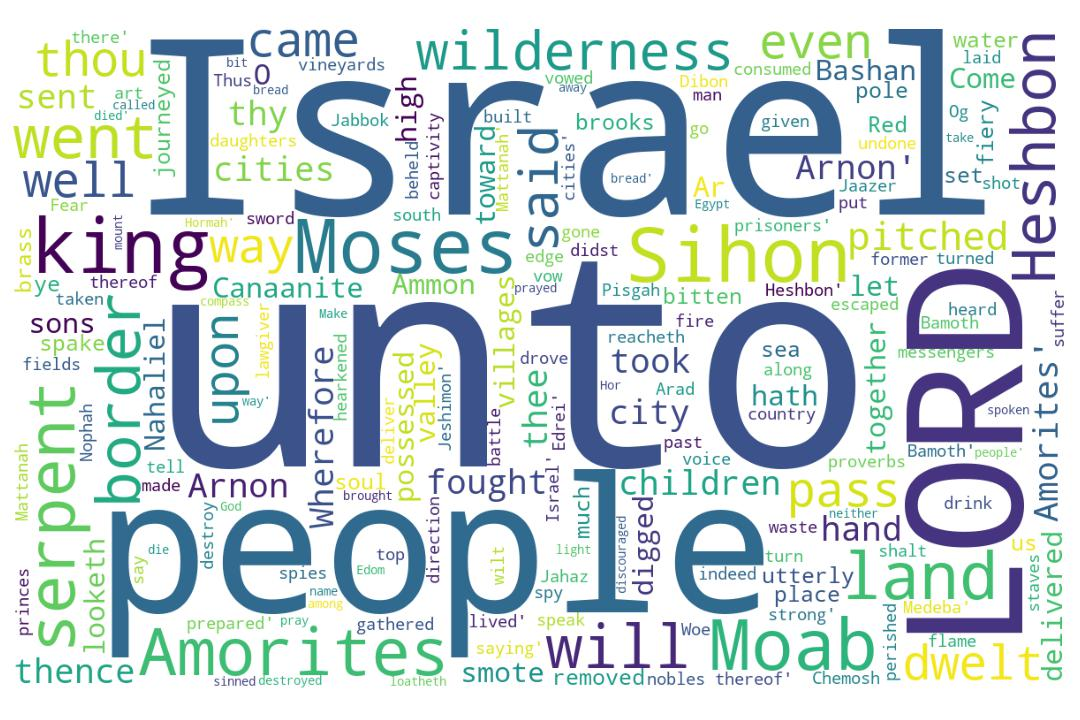
\includegraphics[width=\linewidth]{04OT-Numbers/Numbers21-WordCloud.jpg}
  \caption{Numbers 21 Word Cloud}
  \label{fig:Numbers 21 word Cloud}
\end{figure}


\marginpar{\scriptsize \centering \fcolorbox{bone}{lime}{\textbf{SIN, SERPENTS \& SWORDS}}\\ (Numbers 21)
\begin{compactenum}[I.][8]
     \item  The \textbf{Sin} of Discouragement \index[scripture]{Numbers!Num 21:04}   (Numbers 21:4)
    \item  \textbf{Serpents}  \index[scripture]{Numbers!Num 21:06}   (Numbers 21:6)
    \item  \textbf{Supplication}  \index[scripture]{Numbers!Num 21:07}   (Numbers 21:7)
    \item  The \textbf{Symbol}  \index[scripture]{Numbers!Num 21:09}   (Numbers 21:9)
    \item  A \textbf{Song}  \index[scripture]{Numbers!Num 21:17}   (Numbers 21:17)
    \item  The \textbf{Sword}  \index[scripture]{Numbers!Num 21:24}   (Numbers 21:24)
\end{compactenum}}




\footnote{\textcolor[rgb]{0.00,0.25,0.00}{\hyperlink{NumbersTOC}{Return to end of Table of Contents.}}}\footnote{\href{https://audiobible.com/bible/numbers_21.html}{\textcolor[cmyk]{0.99998,1,0,0}{Numbers 21 Audio}}}\textcolor[cmyk]{0.99998,1,0,0}{And \emph{when} king Arad the Canaanite, which dwelt in the south, heard tell that Israel came by the way of the spies; then he fought against Israel, and took \emph{some} of them prisoners.}
[2] \textcolor[cmyk]{0.99998,1,0,0}{And Israel vowed a vow unto the LORD, and said, If thou wilt indeed deliver this people into my hand, then I will utterly destroy their cities.}
[3] \textcolor[cmyk]{0.99998,1,0,0}{And the LORD hearkened to the voice of Israel, and delivered up the Canaanites; and they utterly destroyed them and their cities: and he called the name of the place Hormah.}\\
\\
\P \textcolor[cmyk]{0.99998,1,0,0}{And they journeyed from mount Hor by the way of the Red sea, to compass the land of Edom: and the soul of the people was much discouraged because of the way.}
[5] \textcolor[cmyk]{0.99998,1,0,0}{And the people spake against God, and against Moses, Wherefore have ye brought us up out of Egypt to die in the wilderness? for \emph{there} \emph{is} no bread, neither \emph{is} \emph{there} \emph{any} water; and our soul loatheth this light bread.}
[6] \textcolor[cmyk]{0.99998,1,0,0}{And the LORD sent fiery serpents among the people, and they bit the people; and much people of Israel died.}\\
\\
\P \textcolor[cmyk]{0.99998,1,0,0}{Therefore the people came to Moses, and said, We have sinned, for we have spoken against the LORD, and against thee; pray unto the LORD, that he take away the serpents from us. And Moses prayed for the people.}
[8] \textcolor[cmyk]{0.99998,1,0,0}{And the LORD said unto Moses, Make thee a fiery serpent, and set it upon a pole: and it shall come to pass, that every one that is bitten, when he looketh upon it, shall live.}
[9] \textcolor[cmyk]{0.99998,1,0,0}{And Moses made a serpent of brass, and put it upon a pole, and it came to pass, that if a serpent had bitten any man, when he beheld the serpent of brass, he lived.}\\
\\
\P \textcolor[cmyk]{0.99998,1,0,0}{And the children of Israel set forward, and pitched in Oboth.}
[11] \textcolor[cmyk]{0.99998,1,0,0}{And they journeyed from Oboth, and pitched at Ije-abarim, in the wilderness which \emph{is} before Moab, toward the sunrising.}
[12] \textcolor[cmyk]{0.99998,1,0,0}{From thence they removed, and pitched in the valley of Zared.}
[13] \textcolor[cmyk]{0.99998,1,0,0}{From thence they removed, and pitched on the other side of Arnon, which \emph{is} in the wilderness that cometh out of the coasts of the Amorites: for Arnon \emph{is} the border of Moab, between Moab and the Amorites.}
[14] \textcolor[cmyk]{0.99998,1,0,0}{Wherefore it is said in the book of the wars of the LORD, What he did in the Red sea, and in the brooks of Arnon,}
[15] \textcolor[cmyk]{0.99998,1,0,0}{And at the stream of the brooks that goeth down to the dwelling of Ar, and lieth upon the border of Moab.}
[16] \textcolor[cmyk]{0.99998,1,0,0}{And from thence \emph{they} \emph{went} to Beer: that \emph{is} the well whereof the LORD spake unto Moses, Gather the people together, and I will give them water.}
[17] \textcolor[cmyk]{0.99998,1,0,0}{Then Israel sang this song, Spring up, O well; sing ye unto it:}
[18] \textcolor[cmyk]{0.99998,1,0,0}{The princes digged the well, the nobles of the people digged it, by \emph{the} \emph{direction} \emph{of} the lawgiver, with their staves. And from the wilderness \emph{they} \emph{went} to Mattanah:}
[19] \textcolor[cmyk]{0.99998,1,0,0}{And from Mattanah to Nahaliel: and from Nahaliel to Bamoth:}
[20] \textcolor[cmyk]{0.99998,1,0,0}{And from Bamoth \emph{in} the valley, that \emph{is} in the country of Moab, to the top of Pisgah, which looketh toward Jeshimon.}\\
\\
\P \textcolor[cmyk]{0.99998,1,0,0}{And Israel sent messengers unto Sihon king of the Amorites, saying,}
[22] \textcolor[cmyk]{0.99998,1,0,0}{Let me pass through thy land: we will not turn into the fields, or into the vineyards; we will not drink \emph{of} the waters of the well: \emph{but} we will go along by the king's \emph{high} way, until we be past thy borders.}
[23] \textcolor[cmyk]{0.99998,1,0,0}{And Sihon would not suffer Israel to pass through \fcolorbox{bone}{bone}{his} border: but Sihon gathered all \fcolorbox{bone}{bone}{his} people together, and went out against Israel into the wilderness: and he came to Jahaz, and fought against Israel.}
[24] \textcolor[cmyk]{0.99998,1,0,0}{And Israel smote him with the edge of the sword, and possessed \fcolorbox{bone}{bone}{his} land from Arnon unto Jabbok, even unto the children of Ammon: for the border of the children of Ammon \emph{was} strong.}
[25] \textcolor[cmyk]{0.99998,1,0,0}{And Israel took all these cities: and Israel dwelt in all the cities of the Amorites, in Heshbon, and in all the villages thereof.}
[26] \textcolor[cmyk]{0.99998,1,0,0}{For Heshbon \emph{was} the city of Sihon the king of the Amorites, who had fought against the former king of Moab, and taken all \fcolorbox{bone}{bone}{his} land out of \fcolorbox{bone}{bone}{his} hand, even unto Arnon.}
[27] \textcolor[cmyk]{0.99998,1,0,0}{Wherefore they that speak in proverbs say, Come into Heshbon, let the city of Sihon be built and prepared:}
[28] \textcolor[cmyk]{0.99998,1,0,0}{For there is a fire gone out of Heshbon, a flame from the city of Sihon: it hath consumed Ar of Moab, \emph{and} the lords of the high places of Arnon.}
[29] \textcolor[cmyk]{0.99998,1,0,0}{Woe to thee, Moab! thou art undone, O people of Chemosh: he hath given \fcolorbox{bone}{bone}{his} sons that escaped, and \fcolorbox{bone}{bone}{his} daughters, into captivity unto Sihon king of the Amorites.}
[30] \textcolor[cmyk]{0.99998,1,0,0}{We have shot at them; Heshbon is perished even unto Dibon, and we have laid them waste even unto Nophah, which \emph{reacheth} unto Medeba.}\\
\\
\P \textcolor[cmyk]{0.99998,1,0,0}{Thus Israel dwelt in the land of the Amorites.}
[32] \textcolor[cmyk]{0.99998,1,0,0}{And Moses sent to spy out Jaazer, and they took the villages thereof, and drove out the Amorites that \emph{were} there.}
[33] \textcolor[cmyk]{0.99998,1,0,0}{And they turned and went up by the way of Bashan: and Og the king of Bashan went out against them, he, and all \fcolorbox{bone}{bone}{his} people, to the battle at Edrei.}
[34] \textcolor[cmyk]{0.99998,1,0,0}{And the LORD said unto Moses, Fear him not: for I have delivered him into thy hand, and all \fcolorbox{bone}{bone}{his} people, and \fcolorbox{bone}{bone}{his} land; and thou shalt do to him as thou didst unto Sihon king of the Amorites, which dwelt at Heshbon.}
[35] \textcolor[cmyk]{0.99998,1,0,0}{So they smote him, and \fcolorbox{bone}{bone}{his} sons, and all \fcolorbox{bone}{bone}{his} people, until there was none left him alive: and they possessed \fcolorbox{bone}{bone}{his} land.}
\index[NWIV]{33!Numbers!Num 21:1}\index[AWIP]{And!Numbers!Num 21:1}\index[AWIP]{\emph{when}!Numbers!Num 21:1}\index[AWIP]{king!Numbers!Num 21:1}\index[AWIP]{Arad!Numbers!Num 21:1}\index[AWIP]{the!Numbers!Num 21:1}\index[AWIP]{the!Numbers!Num 21:1 (2)}\index[AWIP]{the!Numbers!Num 21:1 (3)}\index[AWIP]{the!Numbers!Num 21:1 (4)}\index[AWIP]{Canaanite!Numbers!Num 21:1}\index[AWIP]{which!Numbers!Num 21:1}\index[AWIP]{dwelt!Numbers!Num 21:1}\index[AWIP]{in!Numbers!Num 21:1}\index[AWIP]{south!Numbers!Num 21:1}\index[AWIP]{heard!Numbers!Num 21:1}\index[AWIP]{tell!Numbers!Num 21:1}\index[AWIP]{that!Numbers!Num 21:1}\index[AWIP]{Israel!Numbers!Num 21:1}\index[AWIP]{Israel!Numbers!Num 21:1 (2)}\index[AWIP]{came!Numbers!Num 21:1}\index[AWIP]{by!Numbers!Num 21:1}\index[AWIP]{way!Numbers!Num 21:1}\index[AWIP]{of!Numbers!Num 21:1}\index[AWIP]{of!Numbers!Num 21:1 (2)}\index[AWIP]{spies!Numbers!Num 21:1}\index[AWIP]{then!Numbers!Num 21:1}\index[AWIP]{he!Numbers!Num 21:1}\index[AWIP]{fought!Numbers!Num 21:1}\index[AWIP]{against!Numbers!Num 21:1}\index[AWIP]{and!Numbers!Num 21:1}\index[AWIP]{took!Numbers!Num 21:1}\index[AWIP]{\emph{some}!Numbers!Num 21:1}\index[AWIP]{them!Numbers!Num 21:1}\index[AWIP]{prisoners!Numbers!Num 21:1}\index[AWIP]{\emph{when}!Numbers!Num 21:1}\index[AWIP]{\emph{some}!Numbers!Num 21:1}

\index[NWIV]{27!Numbers!Num 21:2}\index[AWIP]{And!Numbers!Num 21:2}\index[AWIP]{Israel!Numbers!Num 21:2}\index[AWIP]{vowed!Numbers!Num 21:2}\index[AWIP]{a!Numbers!Num 21:2}\index[AWIP]{vow!Numbers!Num 21:2}\index[AWIP]{unto!Numbers!Num 21:2}\index[AWIP]{the!Numbers!Num 21:2}\index[AWIP]{LORD!Numbers!Num 21:2}\index[AWIP]{and!Numbers!Num 21:2}\index[AWIP]{said!Numbers!Num 21:2}\index[AWIP]{If!Numbers!Num 21:2}\index[AWIP]{thou!Numbers!Num 21:2}\index[AWIP]{wilt!Numbers!Num 21:2}\index[AWIP]{indeed!Numbers!Num 21:2}\index[AWIP]{deliver!Numbers!Num 21:2}\index[AWIP]{this!Numbers!Num 21:2}\index[AWIP]{people!Numbers!Num 21:2}\index[AWIP]{into!Numbers!Num 21:2}\index[AWIP]{my!Numbers!Num 21:2}\index[AWIP]{hand!Numbers!Num 21:2}\index[AWIP]{then!Numbers!Num 21:2}\index[AWIP]{I!Numbers!Num 21:2}\index[AWIP]{will!Numbers!Num 21:2}\index[AWIP]{utterly!Numbers!Num 21:2}\index[AWIP]{destroy!Numbers!Num 21:2}\index[AWIP]{their!Numbers!Num 21:2}\index[AWIP]{cities!Numbers!Num 21:2}

\index[NWIV]{31!Numbers!Num 21:3}\index[AWIP]{And!Numbers!Num 21:3}\index[AWIP]{the!Numbers!Num 21:3}\index[AWIP]{the!Numbers!Num 21:3 (2)}\index[AWIP]{the!Numbers!Num 21:3 (3)}\index[AWIP]{the!Numbers!Num 21:3 (4)}\index[AWIP]{the!Numbers!Num 21:3 (5)}\index[AWIP]{LORD!Numbers!Num 21:3}\index[AWIP]{hearkened!Numbers!Num 21:3}\index[AWIP]{to!Numbers!Num 21:3}\index[AWIP]{voice!Numbers!Num 21:3}\index[AWIP]{of!Numbers!Num 21:3}\index[AWIP]{of!Numbers!Num 21:3 (2)}\index[AWIP]{Israel!Numbers!Num 21:3}\index[AWIP]{and!Numbers!Num 21:3}\index[AWIP]{and!Numbers!Num 21:3 (2)}\index[AWIP]{and!Numbers!Num 21:3 (3)}\index[AWIP]{and!Numbers!Num 21:3 (4)}\index[AWIP]{delivered!Numbers!Num 21:3}\index[AWIP]{up!Numbers!Num 21:3}\index[AWIP]{Canaanites!Numbers!Num 21:3}\index[AWIP]{they!Numbers!Num 21:3}\index[AWIP]{utterly!Numbers!Num 21:3}\index[AWIP]{destroyed!Numbers!Num 21:3}\index[AWIP]{them!Numbers!Num 21:3}\index[AWIP]{their!Numbers!Num 21:3}\index[AWIP]{cities!Numbers!Num 21:3}\index[AWIP]{he!Numbers!Num 21:3}\index[AWIP]{called!Numbers!Num 21:3}\index[AWIP]{name!Numbers!Num 21:3}\index[AWIP]{place!Numbers!Num 21:3}\index[AWIP]{Hormah!Numbers!Num 21:3}

\index[NWIV]{32!Numbers!Num 21:4}\index[AWIP]{And!Numbers!Num 21:4}\index[AWIP]{they!Numbers!Num 21:4}\index[AWIP]{journeyed!Numbers!Num 21:4}\index[AWIP]{from!Numbers!Num 21:4}\index[AWIP]{mount!Numbers!Num 21:4}\index[AWIP]{Hor!Numbers!Num 21:4}\index[AWIP]{by!Numbers!Num 21:4}\index[AWIP]{the!Numbers!Num 21:4}\index[AWIP]{the!Numbers!Num 21:4 (2)}\index[AWIP]{the!Numbers!Num 21:4 (3)}\index[AWIP]{the!Numbers!Num 21:4 (4)}\index[AWIP]{the!Numbers!Num 21:4 (5)}\index[AWIP]{the!Numbers!Num 21:4 (6)}\index[AWIP]{way!Numbers!Num 21:4}\index[AWIP]{way!Numbers!Num 21:4 (2)}\index[AWIP]{of!Numbers!Num 21:4}\index[AWIP]{of!Numbers!Num 21:4 (2)}\index[AWIP]{of!Numbers!Num 21:4 (3)}\index[AWIP]{of!Numbers!Num 21:4 (4)}\index[AWIP]{Red!Numbers!Num 21:4}\index[AWIP]{sea!Numbers!Num 21:4}\index[AWIP]{to!Numbers!Num 21:4}\index[AWIP]{compass!Numbers!Num 21:4}\index[AWIP]{land!Numbers!Num 21:4}\index[AWIP]{Edom!Numbers!Num 21:4}\index[AWIP]{and!Numbers!Num 21:4}\index[AWIP]{soul!Numbers!Num 21:4}\index[AWIP]{people!Numbers!Num 21:4}\index[AWIP]{was!Numbers!Num 21:4}\index[AWIP]{much!Numbers!Num 21:4}\index[AWIP]{discouraged!Numbers!Num 21:4}\index[AWIP]{because!Numbers!Num 21:4}

\index[NWIV]{40!Numbers!Num 21:5}\index[AWIP]{And!Numbers!Num 21:5}\index[AWIP]{the!Numbers!Num 21:5}\index[AWIP]{the!Numbers!Num 21:5 (2)}\index[AWIP]{people!Numbers!Num 21:5}\index[AWIP]{spake!Numbers!Num 21:5}\index[AWIP]{against!Numbers!Num 21:5}\index[AWIP]{against!Numbers!Num 21:5 (2)}\index[AWIP]{God!Numbers!Num 21:5}\index[AWIP]{and!Numbers!Num 21:5}\index[AWIP]{and!Numbers!Num 21:5 (2)}\index[AWIP]{Moses!Numbers!Num 21:5}\index[AWIP]{Wherefore!Numbers!Num 21:5}\index[AWIP]{have!Numbers!Num 21:5}\index[AWIP]{ye!Numbers!Num 21:5}\index[AWIP]{brought!Numbers!Num 21:5}\index[AWIP]{us!Numbers!Num 21:5}\index[AWIP]{up!Numbers!Num 21:5}\index[AWIP]{out!Numbers!Num 21:5}\index[AWIP]{of!Numbers!Num 21:5}\index[AWIP]{Egypt!Numbers!Num 21:5}\index[AWIP]{to!Numbers!Num 21:5}\index[AWIP]{die!Numbers!Num 21:5}\index[AWIP]{in!Numbers!Num 21:5}\index[AWIP]{wilderness?!Numbers!Num 21:5}\index[AWIP]{for!Numbers!Num 21:5}\index[AWIP]{\emph{there}!Numbers!Num 21:5}\index[AWIP]{\emph{there}!Numbers!Num 21:5 (2)}\index[AWIP]{\emph{is}!Numbers!Num 21:5}\index[AWIP]{\emph{is}!Numbers!Num 21:5 (2)}\index[AWIP]{no!Numbers!Num 21:5}\index[AWIP]{bread!Numbers!Num 21:5}\index[AWIP]{bread!Numbers!Num 21:5 (2)}\index[AWIP]{neither!Numbers!Num 21:5}\index[AWIP]{\emph{any}!Numbers!Num 21:5}\index[AWIP]{water!Numbers!Num 21:5}\index[AWIP]{our!Numbers!Num 21:5}\index[AWIP]{soul!Numbers!Num 21:5}\index[AWIP]{loatheth!Numbers!Num 21:5}\index[AWIP]{this!Numbers!Num 21:5}\index[AWIP]{light!Numbers!Num 21:5}\index[AWIP]{\emph{there}!Numbers!Num 21:5}\index[AWIP]{\emph{there}!Numbers!Num 21:5 (2)}\index[AWIP]{\emph{is}!Numbers!Num 21:5}\index[AWIP]{\emph{is}!Numbers!Num 21:5 (2)}\index[AWIP]{\emph{any}!Numbers!Num 21:5}

\index[NWIV]{20!Numbers!Num 21:6}\index[AWIP]{And!Numbers!Num 21:6}\index[AWIP]{the!Numbers!Num 21:6}\index[AWIP]{the!Numbers!Num 21:6 (2)}\index[AWIP]{the!Numbers!Num 21:6 (3)}\index[AWIP]{LORD!Numbers!Num 21:6}\index[AWIP]{sent!Numbers!Num 21:6}\index[AWIP]{fiery!Numbers!Num 21:6}\index[AWIP]{serpents!Numbers!Num 21:6}\index[AWIP]{among!Numbers!Num 21:6}\index[AWIP]{people!Numbers!Num 21:6}\index[AWIP]{people!Numbers!Num 21:6 (2)}\index[AWIP]{people!Numbers!Num 21:6 (3)}\index[AWIP]{and!Numbers!Num 21:6}\index[AWIP]{and!Numbers!Num 21:6 (2)}\index[AWIP]{they!Numbers!Num 21:6}\index[AWIP]{bit!Numbers!Num 21:6}\index[AWIP]{much!Numbers!Num 21:6}\index[AWIP]{of!Numbers!Num 21:6}\index[AWIP]{Israel!Numbers!Num 21:6}\index[AWIP]{died!Numbers!Num 21:6}

\index[NWIV]{39!Numbers!Num 21:7}\index[AWIP]{Therefore!Numbers!Num 21:7}\index[AWIP]{the!Numbers!Num 21:7}\index[AWIP]{the!Numbers!Num 21:7 (2)}\index[AWIP]{the!Numbers!Num 21:7 (3)}\index[AWIP]{the!Numbers!Num 21:7 (4)}\index[AWIP]{the!Numbers!Num 21:7 (5)}\index[AWIP]{people!Numbers!Num 21:7}\index[AWIP]{people!Numbers!Num 21:7 (2)}\index[AWIP]{came!Numbers!Num 21:7}\index[AWIP]{to!Numbers!Num 21:7}\index[AWIP]{Moses!Numbers!Num 21:7}\index[AWIP]{Moses!Numbers!Num 21:7 (2)}\index[AWIP]{and!Numbers!Num 21:7}\index[AWIP]{and!Numbers!Num 21:7 (2)}\index[AWIP]{said!Numbers!Num 21:7}\index[AWIP]{We!Numbers!Num 21:7}\index[AWIP]{have!Numbers!Num 21:7}\index[AWIP]{have!Numbers!Num 21:7 (2)}\index[AWIP]{sinned!Numbers!Num 21:7}\index[AWIP]{for!Numbers!Num 21:7}\index[AWIP]{for!Numbers!Num 21:7 (2)}\index[AWIP]{we!Numbers!Num 21:7}\index[AWIP]{spoken!Numbers!Num 21:7}\index[AWIP]{against!Numbers!Num 21:7}\index[AWIP]{against!Numbers!Num 21:7 (2)}\index[AWIP]{LORD!Numbers!Num 21:7}\index[AWIP]{LORD!Numbers!Num 21:7 (2)}\index[AWIP]{thee!Numbers!Num 21:7}\index[AWIP]{pray!Numbers!Num 21:7}\index[AWIP]{unto!Numbers!Num 21:7}\index[AWIP]{that!Numbers!Num 21:7}\index[AWIP]{he!Numbers!Num 21:7}\index[AWIP]{take!Numbers!Num 21:7}\index[AWIP]{away!Numbers!Num 21:7}\index[AWIP]{serpents!Numbers!Num 21:7}\index[AWIP]{from!Numbers!Num 21:7}\index[AWIP]{us!Numbers!Num 21:7}\index[AWIP]{And!Numbers!Num 21:7}\index[AWIP]{prayed!Numbers!Num 21:7}

\index[NWIV]{36!Numbers!Num 21:8}\index[AWIP]{And!Numbers!Num 21:8}\index[AWIP]{the!Numbers!Num 21:8}\index[AWIP]{LORD!Numbers!Num 21:8}\index[AWIP]{said!Numbers!Num 21:8}\index[AWIP]{unto!Numbers!Num 21:8}\index[AWIP]{Moses!Numbers!Num 21:8}\index[AWIP]{Make!Numbers!Num 21:8}\index[AWIP]{thee!Numbers!Num 21:8}\index[AWIP]{a!Numbers!Num 21:8}\index[AWIP]{a!Numbers!Num 21:8 (2)}\index[AWIP]{fiery!Numbers!Num 21:8}\index[AWIP]{serpent!Numbers!Num 21:8}\index[AWIP]{and!Numbers!Num 21:8}\index[AWIP]{and!Numbers!Num 21:8 (2)}\index[AWIP]{set!Numbers!Num 21:8}\index[AWIP]{it!Numbers!Num 21:8}\index[AWIP]{it!Numbers!Num 21:8 (2)}\index[AWIP]{it!Numbers!Num 21:8 (3)}\index[AWIP]{upon!Numbers!Num 21:8}\index[AWIP]{upon!Numbers!Num 21:8 (2)}\index[AWIP]{pole!Numbers!Num 21:8}\index[AWIP]{shall!Numbers!Num 21:8}\index[AWIP]{shall!Numbers!Num 21:8 (2)}\index[AWIP]{come!Numbers!Num 21:8}\index[AWIP]{to!Numbers!Num 21:8}\index[AWIP]{pass!Numbers!Num 21:8}\index[AWIP]{that!Numbers!Num 21:8}\index[AWIP]{that!Numbers!Num 21:8 (2)}\index[AWIP]{every!Numbers!Num 21:8}\index[AWIP]{one!Numbers!Num 21:8}\index[AWIP]{is!Numbers!Num 21:8}\index[AWIP]{bitten!Numbers!Num 21:8}\index[AWIP]{when!Numbers!Num 21:8}\index[AWIP]{he!Numbers!Num 21:8}\index[AWIP]{looketh!Numbers!Num 21:8}\index[AWIP]{live!Numbers!Num 21:8}

\index[NWIV]{35!Numbers!Num 21:9}\index[AWIP]{And!Numbers!Num 21:9}\index[AWIP]{Moses!Numbers!Num 21:9}\index[AWIP]{made!Numbers!Num 21:9}\index[AWIP]{a!Numbers!Num 21:9}\index[AWIP]{a!Numbers!Num 21:9 (2)}\index[AWIP]{a!Numbers!Num 21:9 (3)}\index[AWIP]{serpent!Numbers!Num 21:9}\index[AWIP]{serpent!Numbers!Num 21:9 (2)}\index[AWIP]{serpent!Numbers!Num 21:9 (3)}\index[AWIP]{of!Numbers!Num 21:9}\index[AWIP]{of!Numbers!Num 21:9 (2)}\index[AWIP]{brass!Numbers!Num 21:9}\index[AWIP]{brass!Numbers!Num 21:9 (2)}\index[AWIP]{and!Numbers!Num 21:9}\index[AWIP]{and!Numbers!Num 21:9 (2)}\index[AWIP]{put!Numbers!Num 21:9}\index[AWIP]{it!Numbers!Num 21:9}\index[AWIP]{it!Numbers!Num 21:9 (2)}\index[AWIP]{upon!Numbers!Num 21:9}\index[AWIP]{pole!Numbers!Num 21:9}\index[AWIP]{came!Numbers!Num 21:9}\index[AWIP]{to!Numbers!Num 21:9}\index[AWIP]{pass!Numbers!Num 21:9}\index[AWIP]{that!Numbers!Num 21:9}\index[AWIP]{if!Numbers!Num 21:9}\index[AWIP]{had!Numbers!Num 21:9}\index[AWIP]{bitten!Numbers!Num 21:9}\index[AWIP]{any!Numbers!Num 21:9}\index[AWIP]{man!Numbers!Num 21:9}\index[AWIP]{when!Numbers!Num 21:9}\index[AWIP]{he!Numbers!Num 21:9}\index[AWIP]{he!Numbers!Num 21:9 (2)}\index[AWIP]{beheld!Numbers!Num 21:9}\index[AWIP]{the!Numbers!Num 21:9}\index[AWIP]{lived!Numbers!Num 21:9}

\index[NWIV]{11!Numbers!Num 21:10}\index[AWIP]{And!Numbers!Num 21:10}\index[AWIP]{the!Numbers!Num 21:10}\index[AWIP]{children!Numbers!Num 21:10}\index[AWIP]{of!Numbers!Num 21:10}\index[AWIP]{Israel!Numbers!Num 21:10}\index[AWIP]{set!Numbers!Num 21:10}\index[AWIP]{forward!Numbers!Num 21:10}\index[AWIP]{and!Numbers!Num 21:10}\index[AWIP]{pitched!Numbers!Num 21:10}\index[AWIP]{in!Numbers!Num 21:10}\index[AWIP]{Oboth!Numbers!Num 21:10}

\index[NWIV]{19!Numbers!Num 21:11}\index[AWIP]{And!Numbers!Num 21:11}\index[AWIP]{they!Numbers!Num 21:11}\index[AWIP]{journeyed!Numbers!Num 21:11}\index[AWIP]{from!Numbers!Num 21:11}\index[AWIP]{Oboth!Numbers!Num 21:11}\index[AWIP]{and!Numbers!Num 21:11}\index[AWIP]{pitched!Numbers!Num 21:11}\index[AWIP]{at!Numbers!Num 21:11}\index[AWIP]{Ije-abarim!Numbers!Num 21:11}\index[AWIP]{in!Numbers!Num 21:11}\index[AWIP]{the!Numbers!Num 21:11}\index[AWIP]{the!Numbers!Num 21:11 (2)}\index[AWIP]{wilderness!Numbers!Num 21:11}\index[AWIP]{which!Numbers!Num 21:11}\index[AWIP]{\emph{is}!Numbers!Num 21:11}\index[AWIP]{before!Numbers!Num 21:11}\index[AWIP]{Moab!Numbers!Num 21:11}\index[AWIP]{toward!Numbers!Num 21:11}\index[AWIP]{sunrising!Numbers!Num 21:11}\index[AWIP]{\emph{is}!Numbers!Num 21:11}

\index[NWIV]{11!Numbers!Num 21:12}\index[AWIP]{From!Numbers!Num 21:12}\index[AWIP]{thence!Numbers!Num 21:12}\index[AWIP]{they!Numbers!Num 21:12}\index[AWIP]{removed!Numbers!Num 21:12}\index[AWIP]{and!Numbers!Num 21:12}\index[AWIP]{pitched!Numbers!Num 21:12}\index[AWIP]{in!Numbers!Num 21:12}\index[AWIP]{the!Numbers!Num 21:12}\index[AWIP]{valley!Numbers!Num 21:12}\index[AWIP]{of!Numbers!Num 21:12}\index[AWIP]{Zared!Numbers!Num 21:12}

\index[NWIV]{38!Numbers!Num 21:13}\index[AWIP]{From!Numbers!Num 21:13}\index[AWIP]{thence!Numbers!Num 21:13}\index[AWIP]{they!Numbers!Num 21:13}\index[AWIP]{removed!Numbers!Num 21:13}\index[AWIP]{and!Numbers!Num 21:13}\index[AWIP]{and!Numbers!Num 21:13 (2)}\index[AWIP]{pitched!Numbers!Num 21:13}\index[AWIP]{on!Numbers!Num 21:13}\index[AWIP]{the!Numbers!Num 21:13}\index[AWIP]{the!Numbers!Num 21:13 (2)}\index[AWIP]{the!Numbers!Num 21:13 (3)}\index[AWIP]{the!Numbers!Num 21:13 (4)}\index[AWIP]{the!Numbers!Num 21:13 (5)}\index[AWIP]{the!Numbers!Num 21:13 (6)}\index[AWIP]{other!Numbers!Num 21:13}\index[AWIP]{side!Numbers!Num 21:13}\index[AWIP]{of!Numbers!Num 21:13}\index[AWIP]{of!Numbers!Num 21:13 (2)}\index[AWIP]{of!Numbers!Num 21:13 (3)}\index[AWIP]{of!Numbers!Num 21:13 (4)}\index[AWIP]{Arnon!Numbers!Num 21:13}\index[AWIP]{Arnon!Numbers!Num 21:13 (2)}\index[AWIP]{which!Numbers!Num 21:13}\index[AWIP]{\emph{is}!Numbers!Num 21:13}\index[AWIP]{\emph{is}!Numbers!Num 21:13 (2)}\index[AWIP]{in!Numbers!Num 21:13}\index[AWIP]{wilderness!Numbers!Num 21:13}\index[AWIP]{that!Numbers!Num 21:13}\index[AWIP]{cometh!Numbers!Num 21:13}\index[AWIP]{out!Numbers!Num 21:13}\index[AWIP]{coasts!Numbers!Num 21:13}\index[AWIP]{Amorites!Numbers!Num 21:13}\index[AWIP]{Amorites!Numbers!Num 21:13 (2)}\index[AWIP]{for!Numbers!Num 21:13}\index[AWIP]{border!Numbers!Num 21:13}\index[AWIP]{Moab!Numbers!Num 21:13}\index[AWIP]{Moab!Numbers!Num 21:13 (2)}\index[AWIP]{between!Numbers!Num 21:13}\index[AWIP]{\emph{is}!Numbers!Num 21:13}\index[AWIP]{\emph{is}!Numbers!Num 21:13 (2)}

\index[NWIV]{26!Numbers!Num 21:14}\index[AWIP]{Wherefore!Numbers!Num 21:14}\index[AWIP]{it!Numbers!Num 21:14}\index[AWIP]{is!Numbers!Num 21:14}\index[AWIP]{said!Numbers!Num 21:14}\index[AWIP]{in!Numbers!Num 21:14}\index[AWIP]{in!Numbers!Num 21:14 (2)}\index[AWIP]{in!Numbers!Num 21:14 (3)}\index[AWIP]{the!Numbers!Num 21:14}\index[AWIP]{the!Numbers!Num 21:14 (2)}\index[AWIP]{the!Numbers!Num 21:14 (3)}\index[AWIP]{the!Numbers!Num 21:14 (4)}\index[AWIP]{the!Numbers!Num 21:14 (5)}\index[AWIP]{book!Numbers!Num 21:14}\index[AWIP]{of!Numbers!Num 21:14}\index[AWIP]{of!Numbers!Num 21:14 (2)}\index[AWIP]{of!Numbers!Num 21:14 (3)}\index[AWIP]{wars!Numbers!Num 21:14}\index[AWIP]{LORD!Numbers!Num 21:14}\index[AWIP]{What!Numbers!Num 21:14}\index[AWIP]{he!Numbers!Num 21:14}\index[AWIP]{did!Numbers!Num 21:14}\index[AWIP]{Red!Numbers!Num 21:14}\index[AWIP]{sea!Numbers!Num 21:14}\index[AWIP]{and!Numbers!Num 21:14}\index[AWIP]{brooks!Numbers!Num 21:14}\index[AWIP]{Arnon!Numbers!Num 21:14}

\index[NWIV]{22!Numbers!Num 21:15}\index[AWIP]{And!Numbers!Num 21:15}\index[AWIP]{at!Numbers!Num 21:15}\index[AWIP]{the!Numbers!Num 21:15}\index[AWIP]{the!Numbers!Num 21:15 (2)}\index[AWIP]{the!Numbers!Num 21:15 (3)}\index[AWIP]{the!Numbers!Num 21:15 (4)}\index[AWIP]{stream!Numbers!Num 21:15}\index[AWIP]{of!Numbers!Num 21:15}\index[AWIP]{of!Numbers!Num 21:15 (2)}\index[AWIP]{of!Numbers!Num 21:15 (3)}\index[AWIP]{brooks!Numbers!Num 21:15}\index[AWIP]{that!Numbers!Num 21:15}\index[AWIP]{goeth!Numbers!Num 21:15}\index[AWIP]{down!Numbers!Num 21:15}\index[AWIP]{to!Numbers!Num 21:15}\index[AWIP]{dwelling!Numbers!Num 21:15}\index[AWIP]{Ar!Numbers!Num 21:15}\index[AWIP]{and!Numbers!Num 21:15}\index[AWIP]{lieth!Numbers!Num 21:15}\index[AWIP]{upon!Numbers!Num 21:15}\index[AWIP]{border!Numbers!Num 21:15}\index[AWIP]{Moab!Numbers!Num 21:15}

\index[NWIV]{27!Numbers!Num 21:16}\index[AWIP]{And!Numbers!Num 21:16}\index[AWIP]{from!Numbers!Num 21:16}\index[AWIP]{thence!Numbers!Num 21:16}\index[AWIP]{\emph{they}!Numbers!Num 21:16}\index[AWIP]{\emph{went}!Numbers!Num 21:16}\index[AWIP]{to!Numbers!Num 21:16}\index[AWIP]{Beer!Numbers!Num 21:16}\index[AWIP]{that!Numbers!Num 21:16}\index[AWIP]{\emph{is}!Numbers!Num 21:16}\index[AWIP]{the!Numbers!Num 21:16}\index[AWIP]{the!Numbers!Num 21:16 (2)}\index[AWIP]{the!Numbers!Num 21:16 (3)}\index[AWIP]{well!Numbers!Num 21:16}\index[AWIP]{whereof!Numbers!Num 21:16}\index[AWIP]{LORD!Numbers!Num 21:16}\index[AWIP]{spake!Numbers!Num 21:16}\index[AWIP]{unto!Numbers!Num 21:16}\index[AWIP]{Moses!Numbers!Num 21:16}\index[AWIP]{Gather!Numbers!Num 21:16}\index[AWIP]{people!Numbers!Num 21:16}\index[AWIP]{together!Numbers!Num 21:16}\index[AWIP]{and!Numbers!Num 21:16}\index[AWIP]{I!Numbers!Num 21:16}\index[AWIP]{will!Numbers!Num 21:16}\index[AWIP]{give!Numbers!Num 21:16}\index[AWIP]{them!Numbers!Num 21:16}\index[AWIP]{water!Numbers!Num 21:16}\index[AWIP]{\emph{they}!Numbers!Num 21:16}\index[AWIP]{\emph{went}!Numbers!Num 21:16}\index[AWIP]{\emph{is}!Numbers!Num 21:16}

\index[NWIV]{13!Numbers!Num 21:17}\index[AWIP]{Then!Numbers!Num 21:17}\index[AWIP]{Israel!Numbers!Num 21:17}\index[AWIP]{sang!Numbers!Num 21:17}\index[AWIP]{this!Numbers!Num 21:17}\index[AWIP]{song!Numbers!Num 21:17}\index[AWIP]{Spring!Numbers!Num 21:17}\index[AWIP]{up!Numbers!Num 21:17}\index[AWIP]{O!Numbers!Num 21:17}\index[AWIP]{well!Numbers!Num 21:17}\index[AWIP]{sing!Numbers!Num 21:17}\index[AWIP]{ye!Numbers!Num 21:17}\index[AWIP]{unto!Numbers!Num 21:17}\index[AWIP]{it!Numbers!Num 21:17}

\index[NWIV]{29!Numbers!Num 21:18}\index[AWIP]{The!Numbers!Num 21:18}\index[AWIP]{princes!Numbers!Num 21:18}\index[AWIP]{digged!Numbers!Num 21:18}\index[AWIP]{digged!Numbers!Num 21:18 (2)}\index[AWIP]{the!Numbers!Num 21:18}\index[AWIP]{the!Numbers!Num 21:18 (2)}\index[AWIP]{the!Numbers!Num 21:18 (3)}\index[AWIP]{the!Numbers!Num 21:18 (4)}\index[AWIP]{the!Numbers!Num 21:18 (5)}\index[AWIP]{well!Numbers!Num 21:18}\index[AWIP]{nobles!Numbers!Num 21:18}\index[AWIP]{of!Numbers!Num 21:18}\index[AWIP]{people!Numbers!Num 21:18}\index[AWIP]{it!Numbers!Num 21:18}\index[AWIP]{by!Numbers!Num 21:18}\index[AWIP]{\emph{the}!Numbers!Num 21:18}\index[AWIP]{\emph{direction}!Numbers!Num 21:18}\index[AWIP]{\emph{of}!Numbers!Num 21:18}\index[AWIP]{lawgiver!Numbers!Num 21:18}\index[AWIP]{with!Numbers!Num 21:18}\index[AWIP]{their!Numbers!Num 21:18}\index[AWIP]{staves!Numbers!Num 21:18}\index[AWIP]{And!Numbers!Num 21:18}\index[AWIP]{from!Numbers!Num 21:18}\index[AWIP]{wilderness!Numbers!Num 21:18}\index[AWIP]{\emph{they}!Numbers!Num 21:18}\index[AWIP]{\emph{went}!Numbers!Num 21:18}\index[AWIP]{to!Numbers!Num 21:18}\index[AWIP]{Mattanah!Numbers!Num 21:18}\index[AWIP]{\emph{the}!Numbers!Num 21:18}\index[AWIP]{\emph{direction}!Numbers!Num 21:18}\index[AWIP]{\emph{of}!Numbers!Num 21:18}\index[AWIP]{\emph{they}!Numbers!Num 21:18}\index[AWIP]{\emph{went}!Numbers!Num 21:18}

\index[NWIV]{10!Numbers!Num 21:19}\index[AWIP]{And!Numbers!Num 21:19}\index[AWIP]{from!Numbers!Num 21:19}\index[AWIP]{from!Numbers!Num 21:19 (2)}\index[AWIP]{Mattanah!Numbers!Num 21:19}\index[AWIP]{to!Numbers!Num 21:19}\index[AWIP]{to!Numbers!Num 21:19 (2)}\index[AWIP]{Nahaliel!Numbers!Num 21:19}\index[AWIP]{Nahaliel!Numbers!Num 21:19 (2)}\index[AWIP]{and!Numbers!Num 21:19}\index[AWIP]{Bamoth!Numbers!Num 21:19}

\index[NWIV]{22!Numbers!Num 21:20}\index[AWIP]{And!Numbers!Num 21:20}\index[AWIP]{from!Numbers!Num 21:20}\index[AWIP]{Bamoth!Numbers!Num 21:20}\index[AWIP]{\emph{in}!Numbers!Num 21:20}\index[AWIP]{the!Numbers!Num 21:20}\index[AWIP]{the!Numbers!Num 21:20 (2)}\index[AWIP]{the!Numbers!Num 21:20 (3)}\index[AWIP]{valley!Numbers!Num 21:20}\index[AWIP]{that!Numbers!Num 21:20}\index[AWIP]{\emph{is}!Numbers!Num 21:20}\index[AWIP]{in!Numbers!Num 21:20}\index[AWIP]{country!Numbers!Num 21:20}\index[AWIP]{of!Numbers!Num 21:20}\index[AWIP]{of!Numbers!Num 21:20 (2)}\index[AWIP]{Moab!Numbers!Num 21:20}\index[AWIP]{to!Numbers!Num 21:20}\index[AWIP]{top!Numbers!Num 21:20}\index[AWIP]{Pisgah!Numbers!Num 21:20}\index[AWIP]{which!Numbers!Num 21:20}\index[AWIP]{looketh!Numbers!Num 21:20}\index[AWIP]{toward!Numbers!Num 21:20}\index[AWIP]{Jeshimon!Numbers!Num 21:20}\index[AWIP]{\emph{in}!Numbers!Num 21:20}\index[AWIP]{\emph{is}!Numbers!Num 21:20}

\index[NWIV]{11!Numbers!Num 21:21}\index[AWIP]{And!Numbers!Num 21:21}\index[AWIP]{Israel!Numbers!Num 21:21}\index[AWIP]{sent!Numbers!Num 21:21}\index[AWIP]{messengers!Numbers!Num 21:21}\index[AWIP]{unto!Numbers!Num 21:21}\index[AWIP]{Sihon!Numbers!Num 21:21}\index[AWIP]{king!Numbers!Num 21:21}\index[AWIP]{of!Numbers!Num 21:21}\index[AWIP]{the!Numbers!Num 21:21}\index[AWIP]{Amorites!Numbers!Num 21:21}\index[AWIP]{saying!Numbers!Num 21:21}

\index[NWIV]{43!Numbers!Num 21:22}\index[AWIP]{Let!Numbers!Num 21:22}\index[AWIP]{me!Numbers!Num 21:22}\index[AWIP]{pass!Numbers!Num 21:22}\index[AWIP]{through!Numbers!Num 21:22}\index[AWIP]{thy!Numbers!Num 21:22}\index[AWIP]{thy!Numbers!Num 21:22 (2)}\index[AWIP]{land!Numbers!Num 21:22}\index[AWIP]{we!Numbers!Num 21:22}\index[AWIP]{we!Numbers!Num 21:22 (2)}\index[AWIP]{we!Numbers!Num 21:22 (3)}\index[AWIP]{we!Numbers!Num 21:22 (4)}\index[AWIP]{will!Numbers!Num 21:22}\index[AWIP]{will!Numbers!Num 21:22 (2)}\index[AWIP]{will!Numbers!Num 21:22 (3)}\index[AWIP]{not!Numbers!Num 21:22}\index[AWIP]{not!Numbers!Num 21:22 (2)}\index[AWIP]{turn!Numbers!Num 21:22}\index[AWIP]{into!Numbers!Num 21:22}\index[AWIP]{into!Numbers!Num 21:22 (2)}\index[AWIP]{the!Numbers!Num 21:22}\index[AWIP]{the!Numbers!Num 21:22 (2)}\index[AWIP]{the!Numbers!Num 21:22 (3)}\index[AWIP]{the!Numbers!Num 21:22 (4)}\index[AWIP]{the!Numbers!Num 21:22 (5)}\index[AWIP]{fields!Numbers!Num 21:22}\index[AWIP]{or!Numbers!Num 21:22}\index[AWIP]{vineyards!Numbers!Num 21:22}\index[AWIP]{drink!Numbers!Num 21:22}\index[AWIP]{\emph{of}!Numbers!Num 21:22}\index[AWIP]{waters!Numbers!Num 21:22}\index[AWIP]{of!Numbers!Num 21:22}\index[AWIP]{well!Numbers!Num 21:22}\index[AWIP]{\emph{but}!Numbers!Num 21:22}\index[AWIP]{go!Numbers!Num 21:22}\index[AWIP]{along!Numbers!Num 21:22}\index[AWIP]{by!Numbers!Num 21:22}\index[AWIP]{king's!Numbers!Num 21:22}\index[AWIP]{\emph{high}!Numbers!Num 21:22}\index[AWIP]{way!Numbers!Num 21:22}\index[AWIP]{until!Numbers!Num 21:22}\index[AWIP]{be!Numbers!Num 21:22}\index[AWIP]{past!Numbers!Num 21:22}\index[AWIP]{borders!Numbers!Num 21:22}\index[AWIP]{\emph{of}!Numbers!Num 21:22}\index[AWIP]{\emph{but}!Numbers!Num 21:22}\index[AWIP]{\emph{high}!Numbers!Num 21:22}

\index[NWIV]{35!Numbers!Num 21:23}\index[AWIP]{And!Numbers!Num 21:23}\index[AWIP]{Sihon!Numbers!Num 21:23}\index[AWIP]{Sihon!Numbers!Num 21:23 (2)}\index[AWIP]{would!Numbers!Num 21:23}\index[AWIP]{not!Numbers!Num 21:23}\index[AWIP]{suffer!Numbers!Num 21:23}\index[AWIP]{Israel!Numbers!Num 21:23}\index[AWIP]{Israel!Numbers!Num 21:23 (2)}\index[AWIP]{Israel!Numbers!Num 21:23 (3)}\index[AWIP]{to!Numbers!Num 21:23}\index[AWIP]{to!Numbers!Num 21:23 (2)}\index[AWIP]{pass!Numbers!Num 21:23}\index[AWIP]{through!Numbers!Num 21:23}\index[AWIP]{his!Numbers!Num 21:23}\index[AWIP]{his!Numbers!Num 21:23 (2)}\index[AWIP]{border!Numbers!Num 21:23}\index[AWIP]{but!Numbers!Num 21:23}\index[AWIP]{gathered!Numbers!Num 21:23}\index[AWIP]{all!Numbers!Num 21:23}\index[AWIP]{people!Numbers!Num 21:23}\index[AWIP]{together!Numbers!Num 21:23}\index[AWIP]{and!Numbers!Num 21:23}\index[AWIP]{and!Numbers!Num 21:23 (2)}\index[AWIP]{and!Numbers!Num 21:23 (3)}\index[AWIP]{went!Numbers!Num 21:23}\index[AWIP]{out!Numbers!Num 21:23}\index[AWIP]{against!Numbers!Num 21:23}\index[AWIP]{against!Numbers!Num 21:23 (2)}\index[AWIP]{into!Numbers!Num 21:23}\index[AWIP]{the!Numbers!Num 21:23}\index[AWIP]{wilderness!Numbers!Num 21:23}\index[AWIP]{he!Numbers!Num 21:23}\index[AWIP]{came!Numbers!Num 21:23}\index[AWIP]{Jahaz!Numbers!Num 21:23}\index[AWIP]{fought!Numbers!Num 21:23}

\index[NWIV]{34!Numbers!Num 21:24}\index[AWIP]{And!Numbers!Num 21:24}\index[AWIP]{Israel!Numbers!Num 21:24}\index[AWIP]{smote!Numbers!Num 21:24}\index[AWIP]{him!Numbers!Num 21:24}\index[AWIP]{with!Numbers!Num 21:24}\index[AWIP]{the!Numbers!Num 21:24}\index[AWIP]{the!Numbers!Num 21:24 (2)}\index[AWIP]{the!Numbers!Num 21:24 (3)}\index[AWIP]{the!Numbers!Num 21:24 (4)}\index[AWIP]{the!Numbers!Num 21:24 (5)}\index[AWIP]{edge!Numbers!Num 21:24}\index[AWIP]{of!Numbers!Num 21:24}\index[AWIP]{of!Numbers!Num 21:24 (2)}\index[AWIP]{of!Numbers!Num 21:24 (3)}\index[AWIP]{of!Numbers!Num 21:24 (4)}\index[AWIP]{sword!Numbers!Num 21:24}\index[AWIP]{and!Numbers!Num 21:24}\index[AWIP]{possessed!Numbers!Num 21:24}\index[AWIP]{his!Numbers!Num 21:24}\index[AWIP]{land!Numbers!Num 21:24}\index[AWIP]{from!Numbers!Num 21:24}\index[AWIP]{Arnon!Numbers!Num 21:24}\index[AWIP]{unto!Numbers!Num 21:24}\index[AWIP]{unto!Numbers!Num 21:24 (2)}\index[AWIP]{Jabbok!Numbers!Num 21:24}\index[AWIP]{even!Numbers!Num 21:24}\index[AWIP]{children!Numbers!Num 21:24}\index[AWIP]{children!Numbers!Num 21:24 (2)}\index[AWIP]{Ammon!Numbers!Num 21:24}\index[AWIP]{Ammon!Numbers!Num 21:24 (2)}\index[AWIP]{for!Numbers!Num 21:24}\index[AWIP]{border!Numbers!Num 21:24}\index[AWIP]{\emph{was}!Numbers!Num 21:24}\index[AWIP]{strong!Numbers!Num 21:24}\index[AWIP]{\emph{was}!Numbers!Num 21:24}

\index[NWIV]{24!Numbers!Num 21:25}\index[AWIP]{And!Numbers!Num 21:25}\index[AWIP]{Israel!Numbers!Num 21:25}\index[AWIP]{Israel!Numbers!Num 21:25 (2)}\index[AWIP]{took!Numbers!Num 21:25}\index[AWIP]{all!Numbers!Num 21:25}\index[AWIP]{all!Numbers!Num 21:25 (2)}\index[AWIP]{all!Numbers!Num 21:25 (3)}\index[AWIP]{these!Numbers!Num 21:25}\index[AWIP]{cities!Numbers!Num 21:25}\index[AWIP]{cities!Numbers!Num 21:25 (2)}\index[AWIP]{and!Numbers!Num 21:25}\index[AWIP]{and!Numbers!Num 21:25 (2)}\index[AWIP]{dwelt!Numbers!Num 21:25}\index[AWIP]{in!Numbers!Num 21:25}\index[AWIP]{in!Numbers!Num 21:25 (2)}\index[AWIP]{in!Numbers!Num 21:25 (3)}\index[AWIP]{the!Numbers!Num 21:25}\index[AWIP]{the!Numbers!Num 21:25 (2)}\index[AWIP]{the!Numbers!Num 21:25 (3)}\index[AWIP]{of!Numbers!Num 21:25}\index[AWIP]{Amorites!Numbers!Num 21:25}\index[AWIP]{Heshbon!Numbers!Num 21:25}\index[AWIP]{villages!Numbers!Num 21:25}\index[AWIP]{thereof!Numbers!Num 21:25}

\index[NWIV]{33!Numbers!Num 21:26}\index[AWIP]{For!Numbers!Num 21:26}\index[AWIP]{Heshbon!Numbers!Num 21:26}\index[AWIP]{\emph{was}!Numbers!Num 21:26}\index[AWIP]{the!Numbers!Num 21:26}\index[AWIP]{the!Numbers!Num 21:26 (2)}\index[AWIP]{the!Numbers!Num 21:26 (3)}\index[AWIP]{the!Numbers!Num 21:26 (4)}\index[AWIP]{city!Numbers!Num 21:26}\index[AWIP]{of!Numbers!Num 21:26}\index[AWIP]{of!Numbers!Num 21:26 (2)}\index[AWIP]{of!Numbers!Num 21:26 (3)}\index[AWIP]{of!Numbers!Num 21:26 (4)}\index[AWIP]{Sihon!Numbers!Num 21:26}\index[AWIP]{king!Numbers!Num 21:26}\index[AWIP]{king!Numbers!Num 21:26 (2)}\index[AWIP]{Amorites!Numbers!Num 21:26}\index[AWIP]{who!Numbers!Num 21:26}\index[AWIP]{had!Numbers!Num 21:26}\index[AWIP]{fought!Numbers!Num 21:26}\index[AWIP]{against!Numbers!Num 21:26}\index[AWIP]{former!Numbers!Num 21:26}\index[AWIP]{Moab!Numbers!Num 21:26}\index[AWIP]{and!Numbers!Num 21:26}\index[AWIP]{taken!Numbers!Num 21:26}\index[AWIP]{all!Numbers!Num 21:26}\index[AWIP]{his!Numbers!Num 21:26}\index[AWIP]{his!Numbers!Num 21:26 (2)}\index[AWIP]{land!Numbers!Num 21:26}\index[AWIP]{out!Numbers!Num 21:26}\index[AWIP]{hand!Numbers!Num 21:26}\index[AWIP]{even!Numbers!Num 21:26}\index[AWIP]{unto!Numbers!Num 21:26}\index[AWIP]{Arnon!Numbers!Num 21:26}\index[AWIP]{\emph{was}!Numbers!Num 21:26}

\index[NWIV]{19!Numbers!Num 21:27}\index[AWIP]{Wherefore!Numbers!Num 21:27}\index[AWIP]{they!Numbers!Num 21:27}\index[AWIP]{that!Numbers!Num 21:27}\index[AWIP]{speak!Numbers!Num 21:27}\index[AWIP]{in!Numbers!Num 21:27}\index[AWIP]{proverbs!Numbers!Num 21:27}\index[AWIP]{say!Numbers!Num 21:27}\index[AWIP]{Come!Numbers!Num 21:27}\index[AWIP]{into!Numbers!Num 21:27}\index[AWIP]{Heshbon!Numbers!Num 21:27}\index[AWIP]{let!Numbers!Num 21:27}\index[AWIP]{the!Numbers!Num 21:27}\index[AWIP]{city!Numbers!Num 21:27}\index[AWIP]{of!Numbers!Num 21:27}\index[AWIP]{Sihon!Numbers!Num 21:27}\index[AWIP]{be!Numbers!Num 21:27}\index[AWIP]{built!Numbers!Num 21:27}\index[AWIP]{and!Numbers!Num 21:27}\index[AWIP]{prepared!Numbers!Num 21:27}

\index[NWIV]{31!Numbers!Num 21:28}\index[AWIP]{For!Numbers!Num 21:28}\index[AWIP]{there!Numbers!Num 21:28}\index[AWIP]{is!Numbers!Num 21:28}\index[AWIP]{a!Numbers!Num 21:28}\index[AWIP]{a!Numbers!Num 21:28 (2)}\index[AWIP]{fire!Numbers!Num 21:28}\index[AWIP]{gone!Numbers!Num 21:28}\index[AWIP]{out!Numbers!Num 21:28}\index[AWIP]{of!Numbers!Num 21:28}\index[AWIP]{of!Numbers!Num 21:28 (2)}\index[AWIP]{of!Numbers!Num 21:28 (3)}\index[AWIP]{of!Numbers!Num 21:28 (4)}\index[AWIP]{of!Numbers!Num 21:28 (5)}\index[AWIP]{Heshbon!Numbers!Num 21:28}\index[AWIP]{flame!Numbers!Num 21:28}\index[AWIP]{from!Numbers!Num 21:28}\index[AWIP]{the!Numbers!Num 21:28}\index[AWIP]{the!Numbers!Num 21:28 (2)}\index[AWIP]{the!Numbers!Num 21:28 (3)}\index[AWIP]{city!Numbers!Num 21:28}\index[AWIP]{Sihon!Numbers!Num 21:28}\index[AWIP]{it!Numbers!Num 21:28}\index[AWIP]{hath!Numbers!Num 21:28}\index[AWIP]{consumed!Numbers!Num 21:28}\index[AWIP]{Ar!Numbers!Num 21:28}\index[AWIP]{Moab!Numbers!Num 21:28}\index[AWIP]{\emph{and}!Numbers!Num 21:28}\index[AWIP]{lords!Numbers!Num 21:28}\index[AWIP]{high!Numbers!Num 21:28}\index[AWIP]{places!Numbers!Num 21:28}\index[AWIP]{Arnon!Numbers!Num 21:28}\index[AWIP]{\emph{and}!Numbers!Num 21:28}

\index[NWIV]{29!Numbers!Num 21:29}\index[AWIP]{Woe!Numbers!Num 21:29}\index[AWIP]{to!Numbers!Num 21:29}\index[AWIP]{thee!Numbers!Num 21:29}\index[AWIP]{Moab!!Numbers!Num 21:29}\index[AWIP]{thou!Numbers!Num 21:29}\index[AWIP]{art!Numbers!Num 21:29}\index[AWIP]{undone!Numbers!Num 21:29}\index[AWIP]{O!Numbers!Num 21:29}\index[AWIP]{people!Numbers!Num 21:29}\index[AWIP]{of!Numbers!Num 21:29}\index[AWIP]{of!Numbers!Num 21:29 (2)}\index[AWIP]{Chemosh!Numbers!Num 21:29}\index[AWIP]{he!Numbers!Num 21:29}\index[AWIP]{hath!Numbers!Num 21:29}\index[AWIP]{given!Numbers!Num 21:29}\index[AWIP]{his!Numbers!Num 21:29}\index[AWIP]{his!Numbers!Num 21:29 (2)}\index[AWIP]{sons!Numbers!Num 21:29}\index[AWIP]{that!Numbers!Num 21:29}\index[AWIP]{escaped!Numbers!Num 21:29}\index[AWIP]{and!Numbers!Num 21:29}\index[AWIP]{daughters!Numbers!Num 21:29}\index[AWIP]{into!Numbers!Num 21:29}\index[AWIP]{captivity!Numbers!Num 21:29}\index[AWIP]{unto!Numbers!Num 21:29}\index[AWIP]{Sihon!Numbers!Num 21:29}\index[AWIP]{king!Numbers!Num 21:29}\index[AWIP]{the!Numbers!Num 21:29}\index[AWIP]{Amorites!Numbers!Num 21:29}

\index[NWIV]{24!Numbers!Num 21:30}\index[AWIP]{We!Numbers!Num 21:30}\index[AWIP]{have!Numbers!Num 21:30}\index[AWIP]{have!Numbers!Num 21:30 (2)}\index[AWIP]{shot!Numbers!Num 21:30}\index[AWIP]{at!Numbers!Num 21:30}\index[AWIP]{them!Numbers!Num 21:30}\index[AWIP]{them!Numbers!Num 21:30 (2)}\index[AWIP]{Heshbon!Numbers!Num 21:30}\index[AWIP]{is!Numbers!Num 21:30}\index[AWIP]{perished!Numbers!Num 21:30}\index[AWIP]{even!Numbers!Num 21:30}\index[AWIP]{even!Numbers!Num 21:30 (2)}\index[AWIP]{unto!Numbers!Num 21:30}\index[AWIP]{unto!Numbers!Num 21:30 (2)}\index[AWIP]{unto!Numbers!Num 21:30 (3)}\index[AWIP]{Dibon!Numbers!Num 21:30}\index[AWIP]{and!Numbers!Num 21:30}\index[AWIP]{we!Numbers!Num 21:30}\index[AWIP]{laid!Numbers!Num 21:30}\index[AWIP]{waste!Numbers!Num 21:30}\index[AWIP]{Nophah!Numbers!Num 21:30}\index[AWIP]{which!Numbers!Num 21:30}\index[AWIP]{\emph{reacheth}!Numbers!Num 21:30}\index[AWIP]{Medeba!Numbers!Num 21:30}\index[AWIP]{\emph{reacheth}!Numbers!Num 21:30}

\index[NWIV]{9!Numbers!Num 21:31}\index[AWIP]{Thus!Numbers!Num 21:31}\index[AWIP]{Israel!Numbers!Num 21:31}\index[AWIP]{dwelt!Numbers!Num 21:31}\index[AWIP]{in!Numbers!Num 21:31}\index[AWIP]{the!Numbers!Num 21:31}\index[AWIP]{the!Numbers!Num 21:31 (2)}\index[AWIP]{land!Numbers!Num 21:31}\index[AWIP]{of!Numbers!Num 21:31}\index[AWIP]{Amorites!Numbers!Num 21:31}

\index[NWIV]{21!Numbers!Num 21:32}\index[AWIP]{And!Numbers!Num 21:32}\index[AWIP]{Moses!Numbers!Num 21:32}\index[AWIP]{sent!Numbers!Num 21:32}\index[AWIP]{to!Numbers!Num 21:32}\index[AWIP]{spy!Numbers!Num 21:32}\index[AWIP]{out!Numbers!Num 21:32}\index[AWIP]{out!Numbers!Num 21:32 (2)}\index[AWIP]{Jaazer!Numbers!Num 21:32}\index[AWIP]{and!Numbers!Num 21:32}\index[AWIP]{and!Numbers!Num 21:32 (2)}\index[AWIP]{they!Numbers!Num 21:32}\index[AWIP]{took!Numbers!Num 21:32}\index[AWIP]{the!Numbers!Num 21:32}\index[AWIP]{the!Numbers!Num 21:32 (2)}\index[AWIP]{villages!Numbers!Num 21:32}\index[AWIP]{thereof!Numbers!Num 21:32}\index[AWIP]{drove!Numbers!Num 21:32}\index[AWIP]{Amorites!Numbers!Num 21:32}\index[AWIP]{that!Numbers!Num 21:32}\index[AWIP]{\emph{were}!Numbers!Num 21:32}\index[AWIP]{there!Numbers!Num 21:32}\index[AWIP]{\emph{were}!Numbers!Num 21:32}

\index[NWIV]{31!Numbers!Num 21:33}\index[AWIP]{And!Numbers!Num 21:33}\index[AWIP]{they!Numbers!Num 21:33}\index[AWIP]{turned!Numbers!Num 21:33}\index[AWIP]{and!Numbers!Num 21:33}\index[AWIP]{and!Numbers!Num 21:33 (2)}\index[AWIP]{and!Numbers!Num 21:33 (3)}\index[AWIP]{went!Numbers!Num 21:33}\index[AWIP]{went!Numbers!Num 21:33 (2)}\index[AWIP]{up!Numbers!Num 21:33}\index[AWIP]{by!Numbers!Num 21:33}\index[AWIP]{the!Numbers!Num 21:33}\index[AWIP]{the!Numbers!Num 21:33 (2)}\index[AWIP]{the!Numbers!Num 21:33 (3)}\index[AWIP]{way!Numbers!Num 21:33}\index[AWIP]{of!Numbers!Num 21:33}\index[AWIP]{of!Numbers!Num 21:33 (2)}\index[AWIP]{Bashan!Numbers!Num 21:33}\index[AWIP]{Bashan!Numbers!Num 21:33 (2)}\index[AWIP]{Og!Numbers!Num 21:33}\index[AWIP]{king!Numbers!Num 21:33}\index[AWIP]{out!Numbers!Num 21:33}\index[AWIP]{against!Numbers!Num 21:33}\index[AWIP]{them!Numbers!Num 21:33}\index[AWIP]{he!Numbers!Num 21:33}\index[AWIP]{all!Numbers!Num 21:33}\index[AWIP]{his!Numbers!Num 21:33}\index[AWIP]{people!Numbers!Num 21:33}\index[AWIP]{to!Numbers!Num 21:33}\index[AWIP]{battle!Numbers!Num 21:33}\index[AWIP]{at!Numbers!Num 21:33}\index[AWIP]{Edrei!Numbers!Num 21:33}

\index[NWIV]{43!Numbers!Num 21:34}\index[AWIP]{And!Numbers!Num 21:34}\index[AWIP]{the!Numbers!Num 21:34}\index[AWIP]{the!Numbers!Num 21:34 (2)}\index[AWIP]{LORD!Numbers!Num 21:34}\index[AWIP]{said!Numbers!Num 21:34}\index[AWIP]{unto!Numbers!Num 21:34}\index[AWIP]{unto!Numbers!Num 21:34 (2)}\index[AWIP]{Moses!Numbers!Num 21:34}\index[AWIP]{Fear!Numbers!Num 21:34}\index[AWIP]{him!Numbers!Num 21:34}\index[AWIP]{him!Numbers!Num 21:34 (2)}\index[AWIP]{him!Numbers!Num 21:34 (3)}\index[AWIP]{not!Numbers!Num 21:34}\index[AWIP]{for!Numbers!Num 21:34}\index[AWIP]{I!Numbers!Num 21:34}\index[AWIP]{have!Numbers!Num 21:34}\index[AWIP]{delivered!Numbers!Num 21:34}\index[AWIP]{into!Numbers!Num 21:34}\index[AWIP]{thy!Numbers!Num 21:34}\index[AWIP]{hand!Numbers!Num 21:34}\index[AWIP]{and!Numbers!Num 21:34}\index[AWIP]{and!Numbers!Num 21:34 (2)}\index[AWIP]{and!Numbers!Num 21:34 (3)}\index[AWIP]{all!Numbers!Num 21:34}\index[AWIP]{his!Numbers!Num 21:34}\index[AWIP]{his!Numbers!Num 21:34 (2)}\index[AWIP]{people!Numbers!Num 21:34}\index[AWIP]{land!Numbers!Num 21:34}\index[AWIP]{thou!Numbers!Num 21:34}\index[AWIP]{thou!Numbers!Num 21:34 (2)}\index[AWIP]{shalt!Numbers!Num 21:34}\index[AWIP]{do!Numbers!Num 21:34}\index[AWIP]{to!Numbers!Num 21:34}\index[AWIP]{as!Numbers!Num 21:34}\index[AWIP]{didst!Numbers!Num 21:34}\index[AWIP]{Sihon!Numbers!Num 21:34}\index[AWIP]{king!Numbers!Num 21:34}\index[AWIP]{of!Numbers!Num 21:34}\index[AWIP]{Amorites!Numbers!Num 21:34}\index[AWIP]{which!Numbers!Num 21:34}\index[AWIP]{dwelt!Numbers!Num 21:34}\index[AWIP]{at!Numbers!Num 21:34}\index[AWIP]{Heshbon!Numbers!Num 21:34}

\index[NWIV]{23!Numbers!Num 21:35}\index[AWIP]{So!Numbers!Num 21:35}\index[AWIP]{they!Numbers!Num 21:35}\index[AWIP]{they!Numbers!Num 21:35 (2)}\index[AWIP]{smote!Numbers!Num 21:35}\index[AWIP]{him!Numbers!Num 21:35}\index[AWIP]{him!Numbers!Num 21:35 (2)}\index[AWIP]{and!Numbers!Num 21:35}\index[AWIP]{and!Numbers!Num 21:35 (2)}\index[AWIP]{and!Numbers!Num 21:35 (3)}\index[AWIP]{his!Numbers!Num 21:35}\index[AWIP]{his!Numbers!Num 21:35 (2)}\index[AWIP]{his!Numbers!Num 21:35 (3)}\index[AWIP]{sons!Numbers!Num 21:35}\index[AWIP]{all!Numbers!Num 21:35}\index[AWIP]{people!Numbers!Num 21:35}\index[AWIP]{until!Numbers!Num 21:35}\index[AWIP]{there!Numbers!Num 21:35}\index[AWIP]{was!Numbers!Num 21:35}\index[AWIP]{none!Numbers!Num 21:35}\index[AWIP]{left!Numbers!Num 21:35}\index[AWIP]{alive!Numbers!Num 21:35}\index[AWIP]{possessed!Numbers!Num 21:35}\index[AWIP]{land!Numbers!Num 21:35}


\section{Number 21 Outlines}

\subsection{My Outlines}

\subsubsection{Sin, Serpents \& Swords}
%Practical Wisdom from Proverbs 6:\footnote{03 November 2014, Keith Anthony}
\index[speaker]{Keith Anthony!Numbers 21 (Sin, Serpents \& Swords}
\index[series]{Numbers (Keith Anthony)!Numbers 21 (Sin, Serpents \& Swords)}
\index[date]{2018/02/17!Numbers 21 (Sin, Serpents \& Swords (Keith Anthony)}

\begin{compactenum}[I.]
    \item  The \textbf{Sin} of Discouragement \index[scripture]{Numbers!Num 21:04}   (Numbers 21:4)
    \item  \textbf{Serpents}  \index[scripture]{Numbers!Num 21:06}   (Numbers 21:6)
    \item  \textbf{Supplication}  \index[scripture]{Numbers!Num 21:07}   (Numbers 21:7)
    \item  The \textbf{Symbol}  \index[scripture]{Numbers!Num 21:09}   (Numbers 21:9)
    \item  A \textbf{Song}  \index[scripture]{Numbers!Num 21:17}   (Numbers 21:17)
    \item  The \textbf{Sword}  \index[scripture]{Numbers!Num 21:24}   (Numbers 21:24)
\end{compactenum}




\subsection{Outlines from Others}
\section{Numbers 21 Comments}

\subsection{Numeric Nuggets}
\textbf{13: } Verse 17 has 13 words, 13 unique words.. The word ``his'' is found 13 time sin the chapter.
\subsection{Numbers 21 Repeated Phrases}


%%%%%%%%%%
%%%%%%%%%%
\normalsize
 
\begin{center}
\begin{longtable}{|c|c|}
\caption[Numbers 21 Repeated Phrases]{Numbers 21 Repeated Phrases}\label{table:Repeated Phrases Numbers 21} \\
\hline \multicolumn{1}{|c|}{\textbf{Phrase}} & \multicolumn{1}{c|}{\textbf{Frequency}} \\ \hline 
\endfirsthead
 
\multicolumn{2}{c}
{{\bfseries \tablename\ \thetable{} -- continued from previous page}} \\  
\hline \multicolumn{1}{|c|}{\textbf{Phrase}} & \multicolumn{1}{c|}{\textbf{Frequency}} \\ \hline 
\endhead
 
\hline \multicolumn{2}{c}{{ }} \\ \hline
\endfoot 
of the & 21\\ \hline 
in the & 10\\ \hline 
the LORD & 9\\ \hline 
the Amorites & 9\\ \hline 
the people & 8\\ \hline 
of the Amorites & 7\\ \hline 
And the & 6\\ \hline 
king of & 6\\ \hline 
the wilderness & 5\\ \hline 
of Moab & 5\\ \hline 
all his & 5\\ \hline 
by the & 4\\ \hline 
the way & 4\\ \hline 
And Israel & 4\\ \hline 
And the LORD & 4\\ \hline 
to the & 4\\ \hline 
and they & 4\\ \hline 
out of & 4\\ \hline 
and pitched & 4\\ \hline 
And from & 4\\ \hline 
king of the & 4\\ \hline 
king of the Amorites & 4\\ \hline 
all his people & 4\\ \hline 
his people & 4\\ \hline 
his land & 4\\ \hline 
even unto & 4\\ \hline 
dwelt in & 3\\ \hline 
by the way & 3\\ \hline 
by the way of & 3\\ \hline 
the way of & 3\\ \hline 
way of & 3\\ \hline 
fought against & 3\\ \hline 
against Israel & 3\\ \hline 
unto the & 3\\ \hline 
of Israel & 3\\ \hline 
And they & 3\\ \hline 
in the wilderness & 3\\ \hline 
people and & 3\\ \hline 
came to & 3\\ \hline 
And Moses & 3\\ \hline 
unto Moses & 3\\ \hline 
to pass & 3\\ \hline 
the children & 3\\ \hline 
the children of & 3\\ \hline 
children of & 3\\ \hline 
of Arnon & 3\\ \hline 
the border & 3\\ \hline 
the border of & 3\\ \hline 
border of & 3\\ \hline 
the well & 3\\ \hline 
unto Sihon & 3\\ \hline 
unto Sihon king & 3\\ \hline 
unto Sihon king of & 3\\ \hline 
unto Sihon king of the & 3\\ \hline 
unto Sihon king of the Amorites & 3\\ \hline 
Sihon king & 3\\ \hline 
Sihon king of & 3\\ \hline 
Sihon king of the & 3\\ \hline 
Sihon king of the Amorites & 3\\ \hline 
we will & 3\\ \hline 
into the & 3\\ \hline 
the city & 3\\ \hline 
the city of & 3\\ \hline 
the city of Sihon & 3\\ \hline 
city of & 3\\ \hline 
city of Sihon & 3\\ \hline 
of Sihon & 3\\ \hline 
and his & 3\\ \hline 
and all & 3\\ \hline 
and all his & 3\\ \hline 
and all his people & 3\\ \hline 
\end{longtable}
\end{center}



%%%%%%%%%%
%%%%%%%%%%



\section{Numbers 21 Statistics}


%%%%%%%%%%%%%%%%%%%%%%%%%%%
%%%%% Word Statistics
%%%%%%%%%%%%%%%%%%%%%%%%%%


\normalsize



\subsection{Chapter Word Statistics}


%%%%%%%%%%
%%%%%%%%%%
 
\begin{center}
\begin{longtable}{l|c|c|c|c}
\caption[Stats for Numbers 21]{Stats for Numbers 21} \label{table:Stats for Numbers 21} \\ 
\hline \multicolumn{1}{|c|}{\textbf{Verse(s)}} & \multicolumn{1}{|c|}{\textbf{Count}} & \multicolumn{1}{|c|}{\textbf{Unique}} & \multicolumn{1}{|c|}{\textbf{Italics}} & \multicolumn{1}{|c|}{\textbf{Uniq Italic}}  \\ \hline 
\endfirsthead
 
\multicolumn{5}{c}
{{\bfseries \tablename\ \thetable{} -- continued from previous page}} \\  
\hline \multicolumn{1}{|c|}{\textbf{Verse(s)}} & \multicolumn{1}{|c|}{\textbf{Count}} & \multicolumn{1}{|c|}{\textbf{Unique}} & \multicolumn{1}{|c|}{\textbf{Italics}} & \multicolumn{1}{|c|}{\textbf{Uniq Italic}}  \\ \hline 
\endhead
 
\hline \multicolumn{5}{|r|}{{Continued if needed}} \\ \hline
\endfoot 
1 & 33 & 28 & 2 & 2\\ \hline
2 & 27 & 27 & 0 & 0\\ \hline
3 & 31 & 23 & 0 & 0\\ \hline
4 & 32 & 23 & 0 & 0\\ \hline
5 & 40 & 34 & 5 & 3\\ \hline
6 & 20 & 15 & 0 & 0\\ \hline
7 & 39 & 28 & 0 & 0\\ \hline
8 & 36 & 29 & 0 & 0\\ \hline
9 & 35 & 26 & 0 & 0\\ \hline
10 & 11 & 11 & 0 & 0\\ \hline
11 & 19 & 18 & 1 & 1\\ \hline
12 & 11 & 11 & 0 & 0\\ \hline
13 & 38 & 25 & 2 & 1\\ \hline
14 & 26 & 18 & 0 & 0\\ \hline
15 & 22 & 17 & 0 & 0\\ \hline
16 & 27 & 25 & 3 & 3\\ \hline
17 & 13 & 13 & 0 & 0\\ \hline
18 & 29 & 24 & 5 & 5\\ \hline
19 & 10 & 7 & 0 & 0\\ \hline
20 & 22 & 19 & 2 & 2\\ \hline
21 & 11 & 11 & 0 & 0\\ \hline
22 & 43 & 31 & 3 & 3\\ \hline
23 & 35 & 27 & 0 & 0\\ \hline
24 & 34 & 24 & 1 & 1\\ \hline
25 & 24 & 15 & 0 & 0\\ \hline
26 & 33 & 25 & 1 & 1\\ \hline
27 & 19 & 19 & 0 & 0\\ \hline
28 & 31 & 24 & 1 & 1\\ \hline
29 & 29 & 27 & 0 & 0\\ \hline
30 & 24 & 19 & 1 & 1\\ \hline
31 & 9 & 8 & 0 & 0\\ \hline
32 & 21 & 18 & 1 & 1\\ \hline
33 & 31 & 24 & 0 & 0\\ \hline
34 & 43 & 35 & 0 & 0\\ \hline
35 & 23 & 17 & 0 & 0\\ \hline
\hline \hline
Total & 931 & 310 & 28 & 17



\end{longtable}
\end{center}

%%%%%%%%%%
%%%%%%%%%%
 
\subsection{Words by Frequency}

\begin{center}
\begin{longtable}{l|r}
\caption[Word Frequencies in Numbers 21]{Word Frequencies in Numbers 21} \label{table:WordsIn-Numbers-21} \\ 
\hline \multicolumn{1}{|c|}{\textbf{Word}} & \multicolumn{1}{c|}{\textbf{Frequency}} \\ \hline 
\endfirsthead
 
\multicolumn{2}{c}
{{\bfseries \tablename\ \thetable{} -- continued from previous page}} \\ 
\hline \multicolumn{1}{|c|}{\textbf{Word}} & \multicolumn{1}{c|}{\textbf{Frequency}} \\ \hline 
\endhead
 
\hline \multicolumn{2}{|r|}{{Continued if needed}} \\ \hline
\endfoot
 
\hline \hline
\endlastfoot
the & 91 \\ \hline
of & 50 \\ \hline
and & 47 \\ \hline
And & 23 \\ \hline
to & 18 \\ \hline
in & 15 \\ \hline
Israel & 15 \\ \hline
unto & 15 \\ \hline
people & 15 \\ \hline
his & 13 \\ \hline
that & 12 \\ \hline
they & 11 \\ \hline
he & 10 \\ \hline
from & 10 \\ \hline
against & 9 \\ \hline
LORD & 9 \\ \hline
it & 9 \\ \hline
Amorites & 9 \\ \hline
a & 8 \\ \hline
Moses & 8 \\ \hline
out & 8 \\ \hline
Moab & 8 \\ \hline
Sihon & 8 \\ \hline
all & 8 \\ \hline
king & 7 \\ \hline
into & 7 \\ \hline
land & 7 \\ \hline
\emph{is} & 7 \\ \hline
which & 6 \\ \hline
them & 6 \\ \hline
have & 6 \\ \hline
for & 6 \\ \hline
we & 6 \\ \hline
Arnon & 6 \\ \hline
him & 6 \\ \hline
Heshbon & 6 \\ \hline
by & 5 \\ \hline
way & 5 \\ \hline
said & 5 \\ \hline
will & 5 \\ \hline
wilderness & 5 \\ \hline
at & 5 \\ \hline
dwelt & 4 \\ \hline
came & 4 \\ \hline
thou & 4 \\ \hline
cities & 4 \\ \hline
up & 4 \\ \hline
serpent & 4 \\ \hline
upon & 4 \\ \hline
pass & 4 \\ \hline
is & 4 \\ \hline
pitched & 4 \\ \hline
border & 4 \\ \hline
well & 4 \\ \hline
not & 4 \\ \hline
even & 4 \\ \hline
fought & 3 \\ \hline
took & 3 \\ \hline
this & 3 \\ \hline
hand & 3 \\ \hline
I & 3 \\ \hline
their & 3 \\ \hline
Wherefore & 3 \\ \hline
sent & 3 \\ \hline
thee & 3 \\ \hline
children & 3 \\ \hline
thence & 3 \\ \hline
thy & 3 \\ \hline
went & 3 \\ \hline
city & 3 \\ \hline
there & 3 \\ \hline
then & 2 \\ \hline
utterly & 2 \\ \hline
delivered & 2 \\ \hline
journeyed & 2 \\ \hline
Red & 2 \\ \hline
sea & 2 \\ \hline
soul & 2 \\ \hline
was & 2 \\ \hline
much & 2 \\ \hline
spake & 2 \\ \hline
ye & 2 \\ \hline
us & 2 \\ \hline
\emph{there} & 2 \\ \hline
bread & 2 \\ \hline
water & 2 \\ \hline
fiery & 2 \\ \hline
serpents & 2 \\ \hline
We & 2 \\ \hline
set & 2 \\ \hline
pole & 2 \\ \hline
shall & 2 \\ \hline
bitten & 2 \\ \hline
when & 2 \\ \hline
looketh & 2 \\ \hline
brass & 2 \\ \hline
had & 2 \\ \hline
Oboth & 2 \\ \hline
toward & 2 \\ \hline
From & 2 \\ \hline
removed & 2 \\ \hline
valley & 2 \\ \hline
brooks & 2 \\ \hline
Ar & 2 \\ \hline
\emph{they} & 2 \\ \hline
\emph{went} & 2 \\ \hline
together & 2 \\ \hline
O & 2 \\ \hline
digged & 2 \\ \hline
\emph{of} & 2 \\ \hline
with & 2 \\ \hline
Mattanah & 2 \\ \hline
Nahaliel & 2 \\ \hline
Bamoth & 2 \\ \hline
through & 2 \\ \hline
until & 2 \\ \hline
be & 2 \\ \hline
smote & 2 \\ \hline
possessed & 2 \\ \hline
Ammon & 2 \\ \hline
\emph{was} & 2 \\ \hline
villages & 2 \\ \hline
thereof & 2 \\ \hline
For & 2 \\ \hline
hath & 2 \\ \hline
sons & 2 \\ \hline
Bashan & 2 \\ \hline
\emph{when} & 1 \\ \hline
Arad & 1 \\ \hline
Canaanite & 1 \\ \hline
south & 1 \\ \hline
heard & 1 \\ \hline
tell & 1 \\ \hline
spies & 1 \\ \hline
\emph{some} & 1 \\ \hline
prisoners & 1 \\ \hline
vowed & 1 \\ \hline
vow & 1 \\ \hline
If & 1 \\ \hline
wilt & 1 \\ \hline
indeed & 1 \\ \hline
deliver & 1 \\ \hline
my & 1 \\ \hline
destroy & 1 \\ \hline
hearkened & 1 \\ \hline
voice & 1 \\ \hline
Canaanites & 1 \\ \hline
destroyed & 1 \\ \hline
called & 1 \\ \hline
name & 1 \\ \hline
place & 1 \\ \hline
Hormah & 1 \\ \hline
mount & 1 \\ \hline
Hor & 1 \\ \hline
compass & 1 \\ \hline
Edom & 1 \\ \hline
discouraged & 1 \\ \hline
because & 1 \\ \hline
God & 1 \\ \hline
brought & 1 \\ \hline
Egypt & 1 \\ \hline
die & 1 \\ \hline
no & 1 \\ \hline
neither & 1 \\ \hline
\emph{any} & 1 \\ \hline
our & 1 \\ \hline
loatheth & 1 \\ \hline
light & 1 \\ \hline
among & 1 \\ \hline
bit & 1 \\ \hline
died & 1 \\ \hline
Therefore & 1 \\ \hline
sinned & 1 \\ \hline
spoken & 1 \\ \hline
pray & 1 \\ \hline
take & 1 \\ \hline
away & 1 \\ \hline
prayed & 1 \\ \hline
Make & 1 \\ \hline
come & 1 \\ \hline
every & 1 \\ \hline
one & 1 \\ \hline
live & 1 \\ \hline
made & 1 \\ \hline
put & 1 \\ \hline
if & 1 \\ \hline
any & 1 \\ \hline
man & 1 \\ \hline
beheld & 1 \\ \hline
lived & 1 \\ \hline
forward & 1 \\ \hline
Ije-abarim & 1 \\ \hline
before & 1 \\ \hline
sunrising & 1 \\ \hline
Zared & 1 \\ \hline
on & 1 \\ \hline
other & 1 \\ \hline
side & 1 \\ \hline
cometh & 1 \\ \hline
coasts & 1 \\ \hline
between & 1 \\ \hline
book & 1 \\ \hline
wars & 1 \\ \hline
What & 1 \\ \hline
did & 1 \\ \hline
stream & 1 \\ \hline
goeth & 1 \\ \hline
down & 1 \\ \hline
dwelling & 1 \\ \hline
lieth & 1 \\ \hline
Beer & 1 \\ \hline
whereof & 1 \\ \hline
Gather & 1 \\ \hline
give & 1 \\ \hline
Then & 1 \\ \hline
sang & 1 \\ \hline
song & 1 \\ \hline
Spring & 1 \\ \hline
sing & 1 \\ \hline
The & 1 \\ \hline
princes & 1 \\ \hline
nobles & 1 \\ \hline
\emph{the} & 1 \\ \hline
\emph{direction} & 1 \\ \hline
lawgiver & 1 \\ \hline
staves & 1 \\ \hline
\emph{in} & 1 \\ \hline
country & 1 \\ \hline
top & 1 \\ \hline
Pisgah & 1 \\ \hline
Jeshimon & 1 \\ \hline
messengers & 1 \\ \hline
saying & 1 \\ \hline
Let & 1 \\ \hline
me & 1 \\ \hline
turn & 1 \\ \hline
fields & 1 \\ \hline
or & 1 \\ \hline
vineyards & 1 \\ \hline
drink & 1 \\ \hline
waters & 1 \\ \hline
\emph{but} & 1 \\ \hline
go & 1 \\ \hline
along & 1 \\ \hline
king's & 1 \\ \hline
\emph{high} & 1 \\ \hline
past & 1 \\ \hline
borders & 1 \\ \hline
would & 1 \\ \hline
suffer & 1 \\ \hline
but & 1 \\ \hline
gathered & 1 \\ \hline
Jahaz & 1 \\ \hline
edge & 1 \\ \hline
sword & 1 \\ \hline
Jabbok & 1 \\ \hline
strong & 1 \\ \hline
these & 1 \\ \hline
who & 1 \\ \hline
former & 1 \\ \hline
taken & 1 \\ \hline
speak & 1 \\ \hline
proverbs & 1 \\ \hline
say & 1 \\ \hline
Come & 1 \\ \hline
let & 1 \\ \hline
built & 1 \\ \hline
prepared & 1 \\ \hline
fire & 1 \\ \hline
gone & 1 \\ \hline
flame & 1 \\ \hline
consumed & 1 \\ \hline
\emph{and} & 1 \\ \hline
lords & 1 \\ \hline
high & 1 \\ \hline
places & 1 \\ \hline
Woe & 1 \\ \hline
art & 1 \\ \hline
undone & 1 \\ \hline
Chemosh & 1 \\ \hline
given & 1 \\ \hline
escaped & 1 \\ \hline
daughters & 1 \\ \hline
captivity & 1 \\ \hline
shot & 1 \\ \hline
perished & 1 \\ \hline
Dibon & 1 \\ \hline
laid & 1 \\ \hline
waste & 1 \\ \hline
Nophah & 1 \\ \hline
\emph{reacheth} & 1 \\ \hline
Medeba & 1 \\ \hline
Thus & 1 \\ \hline
spy & 1 \\ \hline
Jaazer & 1 \\ \hline
drove & 1 \\ \hline
\emph{were} & 1 \\ \hline
turned & 1 \\ \hline
Og & 1 \\ \hline
battle & 1 \\ \hline
Edrei & 1 \\ \hline
Fear & 1 \\ \hline
shalt & 1 \\ \hline
do & 1 \\ \hline
as & 1 \\ \hline
didst & 1 \\ \hline
So & 1 \\ \hline
none & 1 \\ \hline
left & 1 \\ \hline
alive & 1 \\ \hline
\end{longtable}
\end{center}



\normalsize



\subsection{Words Alphabetically}

\begin{center}
\begin{longtable}{l|r}
\caption[Word Alphabetically in Numbers 21]{Word Alphabetically in Numbers 21} \label{table:WordsIn-Numbers-21} \\ 
\hline \multicolumn{1}{|c|}{\textbf{Word}} & \multicolumn{1}{c|}{\textbf{Frequency}} \\ \hline 
\endfirsthead
 
\multicolumn{2}{c}
{{\bfseries \tablename\ \thetable{} -- continued from previous page}} \\ 
\hline \multicolumn{1}{|c|}{\textbf{Word}} & \multicolumn{1}{c|}{\textbf{Frequency}} \\ \hline 
\endhead
 
\hline \multicolumn{2}{|r|}{{Continued if needed}} \\ \hline
\endfoot
 
\hline \hline
\endlastfoot
Ammon & 2 \\ \hline
Amorites & 9 \\ \hline
And & 23 \\ \hline
Ar & 2 \\ \hline
Arad & 1 \\ \hline
Arnon & 6 \\ \hline
Bamoth & 2 \\ \hline
Bashan & 2 \\ \hline
Beer & 1 \\ \hline
Canaanite & 1 \\ \hline
Canaanites & 1 \\ \hline
Chemosh & 1 \\ \hline
Come & 1 \\ \hline
Dibon & 1 \\ \hline
Edom & 1 \\ \hline
Edrei & 1 \\ \hline
Egypt & 1 \\ \hline
Fear & 1 \\ \hline
For & 2 \\ \hline
From & 2 \\ \hline
Gather & 1 \\ \hline
God & 1 \\ \hline
Heshbon & 6 \\ \hline
Hor & 1 \\ \hline
Hormah & 1 \\ \hline
I & 3 \\ \hline
If & 1 \\ \hline
Ije-abarim & 1 \\ \hline
Israel & 15 \\ \hline
Jaazer & 1 \\ \hline
Jabbok & 1 \\ \hline
Jahaz & 1 \\ \hline
Jeshimon & 1 \\ \hline
LORD & 9 \\ \hline
Let & 1 \\ \hline
Make & 1 \\ \hline
Mattanah & 2 \\ \hline
Medeba & 1 \\ \hline
Moab & 8 \\ \hline
Moses & 8 \\ \hline
Nahaliel & 2 \\ \hline
Nophah & 1 \\ \hline
O & 2 \\ \hline
Oboth & 2 \\ \hline
Og & 1 \\ \hline
Pisgah & 1 \\ \hline
Red & 2 \\ \hline
Sihon & 8 \\ \hline
So & 1 \\ \hline
Spring & 1 \\ \hline
The & 1 \\ \hline
Then & 1 \\ \hline
Therefore & 1 \\ \hline
Thus & 1 \\ \hline
We & 2 \\ \hline
What & 1 \\ \hline
Wherefore & 3 \\ \hline
Woe & 1 \\ \hline
Zared & 1 \\ \hline
\emph{and} & 1 \\ \hline
\emph{any} & 1 \\ \hline
\emph{but} & 1 \\ \hline
\emph{direction} & 1 \\ \hline
\emph{high} & 1 \\ \hline
\emph{in} & 1 \\ \hline
\emph{is} & 7 \\ \hline
\emph{of} & 2 \\ \hline
\emph{reacheth} & 1 \\ \hline
\emph{some} & 1 \\ \hline
\emph{there} & 2 \\ \hline
\emph{they} & 2 \\ \hline
\emph{the} & 1 \\ \hline
\emph{was} & 2 \\ \hline
\emph{went} & 2 \\ \hline
\emph{were} & 1 \\ \hline
\emph{when} & 1 \\ \hline
a & 8 \\ \hline
against & 9 \\ \hline
alive & 1 \\ \hline
all & 8 \\ \hline
along & 1 \\ \hline
among & 1 \\ \hline
and & 47 \\ \hline
any & 1 \\ \hline
art & 1 \\ \hline
as & 1 \\ \hline
at & 5 \\ \hline
away & 1 \\ \hline
battle & 1 \\ \hline
be & 2 \\ \hline
because & 1 \\ \hline
before & 1 \\ \hline
beheld & 1 \\ \hline
between & 1 \\ \hline
bit & 1 \\ \hline
bitten & 2 \\ \hline
book & 1 \\ \hline
border & 4 \\ \hline
borders & 1 \\ \hline
brass & 2 \\ \hline
bread & 2 \\ \hline
brooks & 2 \\ \hline
brought & 1 \\ \hline
built & 1 \\ \hline
but & 1 \\ \hline
by & 5 \\ \hline
called & 1 \\ \hline
came & 4 \\ \hline
captivity & 1 \\ \hline
children & 3 \\ \hline
cities & 4 \\ \hline
city & 3 \\ \hline
coasts & 1 \\ \hline
come & 1 \\ \hline
cometh & 1 \\ \hline
compass & 1 \\ \hline
consumed & 1 \\ \hline
country & 1 \\ \hline
daughters & 1 \\ \hline
deliver & 1 \\ \hline
delivered & 2 \\ \hline
destroy & 1 \\ \hline
destroyed & 1 \\ \hline
did & 1 \\ \hline
didst & 1 \\ \hline
die & 1 \\ \hline
died & 1 \\ \hline
digged & 2 \\ \hline
discouraged & 1 \\ \hline
do & 1 \\ \hline
down & 1 \\ \hline
drink & 1 \\ \hline
drove & 1 \\ \hline
dwelling & 1 \\ \hline
dwelt & 4 \\ \hline
edge & 1 \\ \hline
escaped & 1 \\ \hline
even & 4 \\ \hline
every & 1 \\ \hline
fields & 1 \\ \hline
fiery & 2 \\ \hline
fire & 1 \\ \hline
flame & 1 \\ \hline
for & 6 \\ \hline
former & 1 \\ \hline
forward & 1 \\ \hline
fought & 3 \\ \hline
from & 10 \\ \hline
gathered & 1 \\ \hline
give & 1 \\ \hline
given & 1 \\ \hline
go & 1 \\ \hline
goeth & 1 \\ \hline
gone & 1 \\ \hline
had & 2 \\ \hline
hand & 3 \\ \hline
hath & 2 \\ \hline
have & 6 \\ \hline
he & 10 \\ \hline
heard & 1 \\ \hline
hearkened & 1 \\ \hline
high & 1 \\ \hline
him & 6 \\ \hline
his & 13 \\ \hline
if & 1 \\ \hline
in & 15 \\ \hline
indeed & 1 \\ \hline
into & 7 \\ \hline
is & 4 \\ \hline
it & 9 \\ \hline
journeyed & 2 \\ \hline
king & 7 \\ \hline
king's & 1 \\ \hline
laid & 1 \\ \hline
land & 7 \\ \hline
lawgiver & 1 \\ \hline
left & 1 \\ \hline
let & 1 \\ \hline
lieth & 1 \\ \hline
light & 1 \\ \hline
live & 1 \\ \hline
lived & 1 \\ \hline
loatheth & 1 \\ \hline
looketh & 2 \\ \hline
lords & 1 \\ \hline
made & 1 \\ \hline
man & 1 \\ \hline
me & 1 \\ \hline
messengers & 1 \\ \hline
mount & 1 \\ \hline
much & 2 \\ \hline
my & 1 \\ \hline
name & 1 \\ \hline
neither & 1 \\ \hline
no & 1 \\ \hline
nobles & 1 \\ \hline
none & 1 \\ \hline
not & 4 \\ \hline
of & 50 \\ \hline
on & 1 \\ \hline
one & 1 \\ \hline
or & 1 \\ \hline
other & 1 \\ \hline
our & 1 \\ \hline
out & 8 \\ \hline
pass & 4 \\ \hline
past & 1 \\ \hline
people & 15 \\ \hline
perished & 1 \\ \hline
pitched & 4 \\ \hline
place & 1 \\ \hline
places & 1 \\ \hline
pole & 2 \\ \hline
possessed & 2 \\ \hline
pray & 1 \\ \hline
prayed & 1 \\ \hline
prepared & 1 \\ \hline
princes & 1 \\ \hline
prisoners & 1 \\ \hline
proverbs & 1 \\ \hline
put & 1 \\ \hline
removed & 2 \\ \hline
said & 5 \\ \hline
sang & 1 \\ \hline
say & 1 \\ \hline
saying & 1 \\ \hline
sea & 2 \\ \hline
sent & 3 \\ \hline
serpent & 4 \\ \hline
serpents & 2 \\ \hline
set & 2 \\ \hline
shall & 2 \\ \hline
shalt & 1 \\ \hline
shot & 1 \\ \hline
side & 1 \\ \hline
sing & 1 \\ \hline
sinned & 1 \\ \hline
smote & 2 \\ \hline
song & 1 \\ \hline
sons & 2 \\ \hline
soul & 2 \\ \hline
south & 1 \\ \hline
spake & 2 \\ \hline
speak & 1 \\ \hline
spies & 1 \\ \hline
spoken & 1 \\ \hline
spy & 1 \\ \hline
staves & 1 \\ \hline
stream & 1 \\ \hline
strong & 1 \\ \hline
suffer & 1 \\ \hline
sunrising & 1 \\ \hline
sword & 1 \\ \hline
take & 1 \\ \hline
taken & 1 \\ \hline
tell & 1 \\ \hline
that & 12 \\ \hline
the & 91 \\ \hline
thee & 3 \\ \hline
their & 3 \\ \hline
them & 6 \\ \hline
then & 2 \\ \hline
thence & 3 \\ \hline
there & 3 \\ \hline
thereof & 2 \\ \hline
these & 1 \\ \hline
they & 11 \\ \hline
this & 3 \\ \hline
thou & 4 \\ \hline
through & 2 \\ \hline
thy & 3 \\ \hline
to & 18 \\ \hline
together & 2 \\ \hline
took & 3 \\ \hline
top & 1 \\ \hline
toward & 2 \\ \hline
turn & 1 \\ \hline
turned & 1 \\ \hline
undone & 1 \\ \hline
until & 2 \\ \hline
unto & 15 \\ \hline
up & 4 \\ \hline
upon & 4 \\ \hline
us & 2 \\ \hline
utterly & 2 \\ \hline
valley & 2 \\ \hline
villages & 2 \\ \hline
vineyards & 1 \\ \hline
voice & 1 \\ \hline
vow & 1 \\ \hline
vowed & 1 \\ \hline
wars & 1 \\ \hline
was & 2 \\ \hline
waste & 1 \\ \hline
water & 2 \\ \hline
waters & 1 \\ \hline
way & 5 \\ \hline
we & 6 \\ \hline
well & 4 \\ \hline
went & 3 \\ \hline
when & 2 \\ \hline
whereof & 1 \\ \hline
which & 6 \\ \hline
who & 1 \\ \hline
wilderness & 5 \\ \hline
will & 5 \\ \hline
wilt & 1 \\ \hline
with & 2 \\ \hline
would & 1 \\ \hline
ye & 2 \\ \hline
\end{longtable}
\end{center}



\normalsize



\subsection{Word Lengths in Chapter}
\normalsize
\begin{longtable}{l|p{3.75in}}
\caption[Words by Length in Numbers 21]{Words by Length in Numbers 21} \label{table:WordsIn-Numbers-21} \\ 
\hline \multicolumn{1}{|c|}{\textbf{Length}} & \multicolumn{1}{c|}{\textbf{Words}} \\ \hline 
\endfirsthead
 
\multicolumn{2}{c}
{{\bfseries \tablename\ \thetable{} -- continued from previous page}} \\ 
\hline \multicolumn{1}{|c|}{\textbf{Length}} & \multicolumn{1}{c|}{\textbf{Words}} \\ \hline 
\endhead
 
\hline \multicolumn{2}{|r|}{{Continued if needed}} \\ \hline
\endfoot
 
\hline \hline
\endlastfoot
1 & a, I, O \\ \hline
2 & in, by, of, he, If, my, to, up, ye, us, \emph{is}, no, We, we, it, is, if, at, on, Ar, \emph{of}, \emph{in}, me, or, go, be, Og, do, as, So \\ \hline
3 & And, the, way, and, vow, Hor, Red, sea, was, God, out, die, for, \emph{any}, our, bit, set, one, put, had, any, man, did, The, \emph{the}, top, Let, thy, not, \emph{but}, his, but, all, him, \emph{was}, For, who, say, let, \emph{and}, Woe, art, spy \\ \hline
4 & \emph{when}, king, Arad, tell, that, came, then, took, \emph{some}, them, unto, LORD, said, thou, wilt, this, into, hand, will, they, name, from, land, Edom, soul, much, have, sent, died, thee, pray, take, away, Make, upon, pole, come, pass, when, live, made, Moab, From, side, book, wars, What, down, \emph{they}, \emph{went}, Beer, well, give, Then, sang, song, sing, with, turn, \emph{high}, past, went, edge, even, city, Come, fire, gone, hath, high, sons, shot, laid, Thus, \emph{were}, Fear, none, left \\ \hline
5 & which, dwelt, south, heard, spies, vowed, their, voice, place, mount, spake, Moses, Egypt, \emph{there}, bread, water, light, fiery, among, shall, every, brass, lived, Oboth, Zared, other, Arnon, goeth, lieth, Sihon, drink, along, until, would, Jahaz, smote, sword, Ammon, these, taken, speak, built, there, flame, lords, given, Dibon, waste, drove, Edrei, shalt, didst, alive \\ \hline
6 & Israel, fought, indeed, people, cities, called, Hormah, sinned, spoken, prayed, bitten, beheld, before, toward, thence, valley, cometh, coasts, border, brooks, stream, Gather, Spring, digged, nobles, staves, Bamoth, Pisgah, saying, fields, waters, king's, suffer, Jabbok, strong, former, places, undone, Nophah, Medeba, Jaazer, turned, Bashan, battle \\ \hline
7 & against, deliver, utterly, destroy, compass, because, brought, neither, serpent, looketh, forward, pitched, removed, between, whereof, princes, country, through, borders, Heshbon, thereof, Chemosh, escaped \\ \hline
8 & loatheth, serpents, children, Amorites, dwelling, together, lawgiver, Mattanah, Nahaliel, Jeshimon, gathered, villages, proverbs, prepared, consumed, perished, \emph{reacheth} \\ \hline
9 & Canaanite, prisoners, hearkened, delivered, destroyed, journeyed, Wherefore, Therefore, sunrising, \emph{direction}, vineyards, possessed, daughters, captivity \\ \hline
10 & Canaanites, wilderness, Ije-abarim, messengers \\ \hline
11 & discouraged \\ \hline
\end{longtable}






%%%%%%%%%%
%%%%%%%%%%
 



%%%%%%%%%%
%%%%%%%%%%
\subsection{Verses with 13 Words in Chapter}
\normalsize
\begin{longtable}{l|p{3.75in}}
\caption[Verses with 13 Words  in Numbers 21]{Verses with 13 Words  in Numbers 21} \label{table:Verses with 13 Words in-Numbers-21} \\ 
\hline \multicolumn{1}{|c|}{\textbf{Reference}} & \multicolumn{1}{c|}{\textbf{Verse}} \\ \hline 
\endfirsthead
 
\multicolumn{2}{c}
{{\bfseries \tablename\ \thetable{} -- continued from previous page}} \\ 
\hline \multicolumn{1}{|c|}{\textbf{Reference}} & \multicolumn{1}{c|}{\textbf{Verse}} \\ \hline 
\endhead
 
\hline \multicolumn{2}{|r|}{{Continued if needed}} \\ \hline
\endfoot
 
\hline \hline
\endlastfoot
Numbers 21:17 & Then Israel sang this song, Spring up, O well; sing ye unto it: \\ \hline
\end{longtable}






%%%%%%%%%%
%%%%%%%%%%

\chapter{Psalm 48}

\begin{figure}
  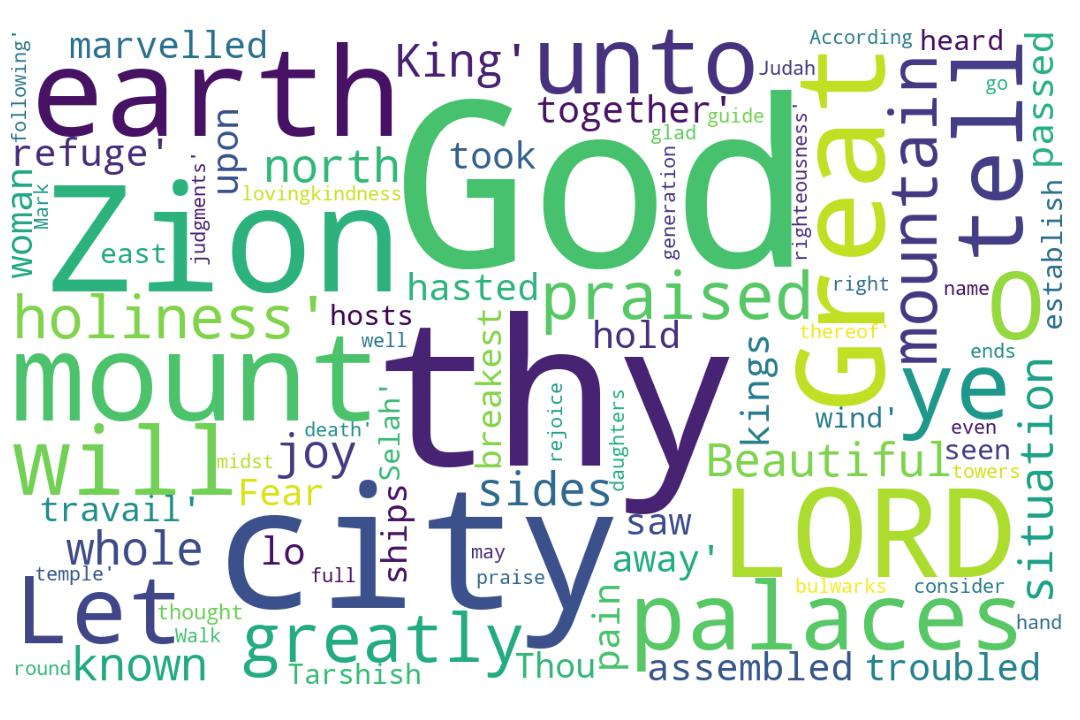
\includegraphics[width=\linewidth]{19OT-Psalms/Psalm48-WordCloud.jpg}
  \caption{Psalm 48 Word Cloud}
  \label{fig:Psalm 48 word Cloud}
\end{figure}



\marginpar{\scriptsize \centering \fcolorbox{bone}{lime}{\textbf{GOD, HIS THRONE, HIS CITY}}\\ (Psalm 48:1-14) \begin{compactenum}[I.][8]
    \item His \textbf{Greatness} \index[scripture]{Psalms!Psa 048:01}(Psa 48:1)
    \item His \textbf{Geography} \index[scripture]{Psalms!Psa 048:02}(Psa 48:2)
    \item Our \textbf{Refuge} \index[scripture]{Psalms!Psa 048:03}(Psa 48:3)
    \item His \textbf{Goodness} \index[scripture]{Psalms!Psa 048:09}(Psa 48:9)
    \item Our \textbf{Gladness} \index[scripture]{Psalms!Psa 048:11}(Psa 48:11)
    \item His \textbf{Glorification} \index[scripture]{Psalms!Psa 048:10}(Psa 48:10)
    \item Our \textbf{Guide} \index[scripture]{Psalms!Psa 048:14}(Psa 48:14)
\end{compactenum}}
    
%%%%%%%%%%%%%%%%%%%%%%%%%%%%%%
%%%%%%%%%%%%%%%%%%%%%%%%%%%%%%
\footnote{\textcolor[cmyk]{0.99998,1,0,0}{\hyperlink{TOC}{Return to end of Table of Contents.}}}\footnote{\href{https://audiobible.com/bible/psalms_48.html}{\textcolor[cmyk]{0.99998,1,0,0}{Psalms Audio}}}\textcolor[cmyk]{0.99998,1,0,0}{A Song \emph{and} Psalm for the sons of Korah.}\\
\\
\textcolor[cmyk]{0.99998,1,0,0}{\fcolorbox{bone}{lime}{Great} \emph{is} the LORD, and greatly to be praised in the city of our God, \emph{in} the mountain of his holiness.}
[2] \textcolor[cmyk]{0.99998,1,0,0}{Beautiful for situation, the joy of the \fcolorbox{bone}{lime}{whole earth}, \emph{is} mount Zion, \emph{on} the sides of the north, the city of the great King.}
[3] \textcolor[cmyk]{0.99998,1,0,0}{God is known in her palaces for a \fcolorbox{bone}{lime}{refuge}.}
[4] \textcolor[cmyk]{0.99998,1,0,0}{For, lo, the kings were assembled, they passed by together.}
[5] \textcolor[cmyk]{0.99998,1,0,0}{They saw \emph{it,} \emph{and} so they marvelled; they were troubled, \emph{and} hasted away.}
[6] \textcolor[cmyk]{0.99998,1,0,0}{Fear took hold upon them there, \emph{and} pain, as of a woman in travail.}
[7] \textcolor[cmyk]{0.99998,1,0,0}{Thou breakest the ships of Tarshish with an east wind.}
[8] \textcolor[cmyk]{0.99998,1,0,0}{As we have heard, so have we seen in the city of the LORD of hosts, in the city of our God: God will establish it for ever. Selah.}
[9] \textcolor[cmyk]{0.99998,1,0,0}{We have thought of thy \fcolorbox{bone}{lime}{lovingkindness}, O God, in the midst of thy temple.}
[10] \textcolor[cmyk]{0.99998,1,0,0}{According to thy name, O God, so \emph{is} thy \fcolorbox{bone}{lime}{praise} unto the ends of the earth: thy right hand is full of \fcolorbox{bone}{MYGOLD}{righteousness}.}
[11] \textcolor[cmyk]{0.99998,1,0,0}{Let mount Zion rejoice, let the daughters of Judah be \fcolorbox{bone}{lime}{glad}, because of thy judgments.}
[12] \textcolor[cmyk]{0.99998,1,0,0}{Walk about Zion, and go round about her: tell the towers thereof.}
[13] \textcolor[cmyk]{0.99998,1,0,0}{Mark ye well her bulwarks, consider her palaces; that ye may tell \emph{it} to the generation following.}
[14] \textcolor[cmyk]{0.99998,1,0,0}{For this God \emph{is} our God for ever and ever: he will be our \fcolorbox{bone}{lime}{guide} \emph{even} unto death.}
\index[NWIV]{21!Psalms!Psa 48:1}\index[AWIP]{Great!Psalms!Psa 48:1}\index[AWIP]{\emph{is}!Psalms!Psa 48:1}\index[AWIP]{the!Psalms!Psa 48:1}\index[AWIP]{the!Psalms!Psa 48:1 (2)}\index[AWIP]{the!Psalms!Psa 48:1 (3)}\index[AWIP]{LORD!Psalms!Psa 48:1}\index[AWIP]{and!Psalms!Psa 48:1}\index[AWIP]{greatly!Psalms!Psa 48:1}\index[AWIP]{to!Psalms!Psa 48:1}\index[AWIP]{be!Psalms!Psa 48:1}\index[AWIP]{praised!Psalms!Psa 48:1}\index[AWIP]{in!Psalms!Psa 48:1}\index[AWIP]{city!Psalms!Psa 48:1}\index[AWIP]{of!Psalms!Psa 48:1}\index[AWIP]{of!Psalms!Psa 48:1 (2)}\index[AWIP]{our!Psalms!Psa 48:1}\index[AWIP]{God!Psalms!Psa 48:1}\index[AWIP]{\emph{in}!Psalms!Psa 48:1}\index[AWIP]{mountain!Psalms!Psa 48:1}\index[AWIP]{his!Psalms!Psa 48:1}\index[AWIP]{holiness!Psalms!Psa 48:1}\index[AWIP]{\emph{is}!Psalms!Psa 48:1}\index[AWIP]{\emph{in}!Psalms!Psa 48:1}

\index[NWIV]{24!Psalms!Psa 48:2}\index[AWIP]{Beautiful!Psalms!Psa 48:2}\index[AWIP]{for!Psalms!Psa 48:2}\index[AWIP]{situation!Psalms!Psa 48:2}\index[AWIP]{the!Psalms!Psa 48:2}\index[AWIP]{the!Psalms!Psa 48:2 (2)}\index[AWIP]{the!Psalms!Psa 48:2 (3)}\index[AWIP]{the!Psalms!Psa 48:2 (4)}\index[AWIP]{the!Psalms!Psa 48:2 (5)}\index[AWIP]{the!Psalms!Psa 48:2 (6)}\index[AWIP]{joy!Psalms!Psa 48:2}\index[AWIP]{of!Psalms!Psa 48:2}\index[AWIP]{of!Psalms!Psa 48:2 (2)}\index[AWIP]{of!Psalms!Psa 48:2 (3)}\index[AWIP]{whole!Psalms!Psa 48:2}\index[AWIP]{earth!Psalms!Psa 48:2}\index[AWIP]{\emph{is}!Psalms!Psa 48:2}\index[AWIP]{mount!Psalms!Psa 48:2}\index[AWIP]{Zion!Psalms!Psa 48:2}\index[AWIP]{\emph{on}!Psalms!Psa 48:2}\index[AWIP]{sides!Psalms!Psa 48:2}\index[AWIP]{north!Psalms!Psa 48:2}\index[AWIP]{city!Psalms!Psa 48:2}\index[AWIP]{great!Psalms!Psa 48:2}\index[AWIP]{King!Psalms!Psa 48:2}\index[AWIP]{\emph{is}!Psalms!Psa 48:2}\index[AWIP]{\emph{on}!Psalms!Psa 48:2}

\index[NWIV]{9!Psalms!Psa 48:3}\index[AWIP]{God!Psalms!Psa 48:3}\index[AWIP]{is!Psalms!Psa 48:3}\index[AWIP]{known!Psalms!Psa 48:3}\index[AWIP]{in!Psalms!Psa 48:3}\index[AWIP]{her!Psalms!Psa 48:3}\index[AWIP]{palaces!Psalms!Psa 48:3}\index[AWIP]{for!Psalms!Psa 48:3}\index[AWIP]{a!Psalms!Psa 48:3}\index[AWIP]{refuge!Psalms!Psa 48:3}

\index[NWIV]{10!Psalms!Psa 48:4}\index[AWIP]{For!Psalms!Psa 48:4}\index[AWIP]{lo!Psalms!Psa 48:4}\index[AWIP]{the!Psalms!Psa 48:4}\index[AWIP]{kings!Psalms!Psa 48:4}\index[AWIP]{were!Psalms!Psa 48:4}\index[AWIP]{assembled!Psalms!Psa 48:4}\index[AWIP]{they!Psalms!Psa 48:4}\index[AWIP]{passed!Psalms!Psa 48:4}\index[AWIP]{by!Psalms!Psa 48:4}\index[AWIP]{together!Psalms!Psa 48:4}

\index[NWIV]{13!Psalms!Psa 48:5}\index[AWIP]{They!Psalms!Psa 48:5}\index[AWIP]{saw!Psalms!Psa 48:5}\index[AWIP]{\emph{it}!Psalms!Psa 48:5}\index[AWIP]{\emph{and}!Psalms!Psa 48:5}\index[AWIP]{\emph{and}!Psalms!Psa 48:5 (2)}\index[AWIP]{so!Psalms!Psa 48:5}\index[AWIP]{they!Psalms!Psa 48:5}\index[AWIP]{they!Psalms!Psa 48:5 (2)}\index[AWIP]{marvelled!Psalms!Psa 48:5}\index[AWIP]{were!Psalms!Psa 48:5}\index[AWIP]{troubled!Psalms!Psa 48:5}\index[AWIP]{hasted!Psalms!Psa 48:5}\index[AWIP]{away!Psalms!Psa 48:5}\index[AWIP]{\emph{it}!Psalms!Psa 48:5}\index[AWIP]{\emph{and}!Psalms!Psa 48:5}\index[AWIP]{\emph{and}!Psalms!Psa 48:5 (2)}

\index[NWIV]{14!Psalms!Psa 48:6}\index[AWIP]{Fear!Psalms!Psa 48:6}\index[AWIP]{took!Psalms!Psa 48:6}\index[AWIP]{hold!Psalms!Psa 48:6}\index[AWIP]{upon!Psalms!Psa 48:6}\index[AWIP]{them!Psalms!Psa 48:6}\index[AWIP]{there!Psalms!Psa 48:6}\index[AWIP]{\emph{and}!Psalms!Psa 48:6}\index[AWIP]{pain!Psalms!Psa 48:6}\index[AWIP]{as!Psalms!Psa 48:6}\index[AWIP]{of!Psalms!Psa 48:6}\index[AWIP]{a!Psalms!Psa 48:6}\index[AWIP]{woman!Psalms!Psa 48:6}\index[AWIP]{in!Psalms!Psa 48:6}\index[AWIP]{travail!Psalms!Psa 48:6}\index[AWIP]{\emph{and}!Psalms!Psa 48:6}

\index[NWIV]{10!Psalms!Psa 48:7}\index[AWIP]{Thou!Psalms!Psa 48:7}\index[AWIP]{breakest!Psalms!Psa 48:7}\index[AWIP]{the!Psalms!Psa 48:7}\index[AWIP]{ships!Psalms!Psa 48:7}\index[AWIP]{of!Psalms!Psa 48:7}\index[AWIP]{Tarshish!Psalms!Psa 48:7}\index[AWIP]{with!Psalms!Psa 48:7}\index[AWIP]{an!Psalms!Psa 48:7}\index[AWIP]{east!Psalms!Psa 48:7}\index[AWIP]{wind!Psalms!Psa 48:7}

\index[NWIV]{29!Psalms!Psa 48:8}\index[AWIP]{As!Psalms!Psa 48:8}\index[AWIP]{we!Psalms!Psa 48:8}\index[AWIP]{we!Psalms!Psa 48:8 (2)}\index[AWIP]{have!Psalms!Psa 48:8}\index[AWIP]{have!Psalms!Psa 48:8 (2)}\index[AWIP]{heard!Psalms!Psa 48:8}\index[AWIP]{so!Psalms!Psa 48:8}\index[AWIP]{seen!Psalms!Psa 48:8}\index[AWIP]{in!Psalms!Psa 48:8}\index[AWIP]{in!Psalms!Psa 48:8 (2)}\index[AWIP]{the!Psalms!Psa 48:8}\index[AWIP]{the!Psalms!Psa 48:8 (2)}\index[AWIP]{the!Psalms!Psa 48:8 (3)}\index[AWIP]{city!Psalms!Psa 48:8}\index[AWIP]{city!Psalms!Psa 48:8 (2)}\index[AWIP]{of!Psalms!Psa 48:8}\index[AWIP]{of!Psalms!Psa 48:8 (2)}\index[AWIP]{of!Psalms!Psa 48:8 (3)}\index[AWIP]{LORD!Psalms!Psa 48:8}\index[AWIP]{hosts!Psalms!Psa 48:8}\index[AWIP]{our!Psalms!Psa 48:8}\index[AWIP]{God!Psalms!Psa 48:8}\index[AWIP]{God!Psalms!Psa 48:8 (2)}\index[AWIP]{will!Psalms!Psa 48:8}\index[AWIP]{establish!Psalms!Psa 48:8}\index[AWIP]{it!Psalms!Psa 48:8}\index[AWIP]{for!Psalms!Psa 48:8}\index[AWIP]{ever!Psalms!Psa 48:8}\index[AWIP]{Selah!Psalms!Psa 48:8}

\index[NWIV]{14!Psalms!Psa 48:9}\index[AWIP]{We!Psalms!Psa 48:9}\index[AWIP]{have!Psalms!Psa 48:9}\index[AWIP]{thought!Psalms!Psa 48:9}\index[AWIP]{of!Psalms!Psa 48:9}\index[AWIP]{of!Psalms!Psa 48:9 (2)}\index[AWIP]{thy!Psalms!Psa 48:9}\index[AWIP]{thy!Psalms!Psa 48:9 (2)}\index[AWIP]{lovingkindness!Psalms!Psa 48:9}\index[AWIP]{O!Psalms!Psa 48:9}\index[AWIP]{God!Psalms!Psa 48:9}\index[AWIP]{in!Psalms!Psa 48:9}\index[AWIP]{the!Psalms!Psa 48:9}\index[AWIP]{midst!Psalms!Psa 48:9}\index[AWIP]{temple!Psalms!Psa 48:9}

\index[NWIV]{23!Psalms!Psa 48:10}\index[AWIP]{According!Psalms!Psa 48:10}\index[AWIP]{to!Psalms!Psa 48:10}\index[AWIP]{thy!Psalms!Psa 48:10}\index[AWIP]{thy!Psalms!Psa 48:10 (2)}\index[AWIP]{thy!Psalms!Psa 48:10 (3)}\index[AWIP]{name!Psalms!Psa 48:10}\index[AWIP]{O!Psalms!Psa 48:10}\index[AWIP]{God!Psalms!Psa 48:10}\index[AWIP]{so!Psalms!Psa 48:10}\index[AWIP]{\emph{is}!Psalms!Psa 48:10}\index[AWIP]{praise!Psalms!Psa 48:10}\index[AWIP]{unto!Psalms!Psa 48:10}\index[AWIP]{the!Psalms!Psa 48:10}\index[AWIP]{the!Psalms!Psa 48:10 (2)}\index[AWIP]{ends!Psalms!Psa 48:10}\index[AWIP]{of!Psalms!Psa 48:10}\index[AWIP]{of!Psalms!Psa 48:10 (2)}\index[AWIP]{earth!Psalms!Psa 48:10}\index[AWIP]{right!Psalms!Psa 48:10}\index[AWIP]{hand!Psalms!Psa 48:10}\index[AWIP]{is!Psalms!Psa 48:10}\index[AWIP]{full!Psalms!Psa 48:10}\index[AWIP]{righteousness!Psalms!Psa 48:10}\index[AWIP]{\emph{is}!Psalms!Psa 48:10}

\index[NWIV]{15!Psalms!Psa 48:11}\index[AWIP]{Let!Psalms!Psa 48:11}\index[AWIP]{mount!Psalms!Psa 48:11}\index[AWIP]{Zion!Psalms!Psa 48:11}\index[AWIP]{rejoice!Psalms!Psa 48:11}\index[AWIP]{let!Psalms!Psa 48:11}\index[AWIP]{the!Psalms!Psa 48:11}\index[AWIP]{daughters!Psalms!Psa 48:11}\index[AWIP]{of!Psalms!Psa 48:11}\index[AWIP]{of!Psalms!Psa 48:11 (2)}\index[AWIP]{Judah!Psalms!Psa 48:11}\index[AWIP]{be!Psalms!Psa 48:11}\index[AWIP]{glad!Psalms!Psa 48:11}\index[AWIP]{because!Psalms!Psa 48:11}\index[AWIP]{thy!Psalms!Psa 48:11}\index[AWIP]{judgments!Psalms!Psa 48:11}

\index[NWIV]{12!Psalms!Psa 48:12}\index[AWIP]{Walk!Psalms!Psa 48:12}\index[AWIP]{about!Psalms!Psa 48:12}\index[AWIP]{about!Psalms!Psa 48:12 (2)}\index[AWIP]{Zion!Psalms!Psa 48:12}\index[AWIP]{and!Psalms!Psa 48:12}\index[AWIP]{go!Psalms!Psa 48:12}\index[AWIP]{round!Psalms!Psa 48:12}\index[AWIP]{her!Psalms!Psa 48:12}\index[AWIP]{tell!Psalms!Psa 48:12}\index[AWIP]{the!Psalms!Psa 48:12}\index[AWIP]{towers!Psalms!Psa 48:12}\index[AWIP]{thereof!Psalms!Psa 48:12}

\index[NWIV]{17!Psalms!Psa 48:13}\index[AWIP]{Mark!Psalms!Psa 48:13}\index[AWIP]{ye!Psalms!Psa 48:13}\index[AWIP]{ye!Psalms!Psa 48:13 (2)}\index[AWIP]{well!Psalms!Psa 48:13}\index[AWIP]{her!Psalms!Psa 48:13}\index[AWIP]{her!Psalms!Psa 48:13 (2)}\index[AWIP]{bulwarks!Psalms!Psa 48:13}\index[AWIP]{consider!Psalms!Psa 48:13}\index[AWIP]{palaces!Psalms!Psa 48:13}\index[AWIP]{that!Psalms!Psa 48:13}\index[AWIP]{may!Psalms!Psa 48:13}\index[AWIP]{tell!Psalms!Psa 48:13}\index[AWIP]{\emph{it}!Psalms!Psa 48:13}\index[AWIP]{to!Psalms!Psa 48:13}\index[AWIP]{the!Psalms!Psa 48:13}\index[AWIP]{generation!Psalms!Psa 48:13}\index[AWIP]{following!Psalms!Psa 48:13}\index[AWIP]{\emph{it}!Psalms!Psa 48:13}

\index[NWIV]{18!Psalms!Psa 48:14}\index[AWIP]{For!Psalms!Psa 48:14}\index[AWIP]{this!Psalms!Psa 48:14}\index[AWIP]{God!Psalms!Psa 48:14}\index[AWIP]{God!Psalms!Psa 48:14 (2)}\index[AWIP]{\emph{is}!Psalms!Psa 48:14}\index[AWIP]{our!Psalms!Psa 48:14}\index[AWIP]{our!Psalms!Psa 48:14 (2)}\index[AWIP]{for!Psalms!Psa 48:14}\index[AWIP]{ever!Psalms!Psa 48:14}\index[AWIP]{ever!Psalms!Psa 48:14 (2)}\index[AWIP]{and!Psalms!Psa 48:14}\index[AWIP]{he!Psalms!Psa 48:14}\index[AWIP]{will!Psalms!Psa 48:14}\index[AWIP]{be!Psalms!Psa 48:14}\index[AWIP]{guide!Psalms!Psa 48:14}\index[AWIP]{\emph{even}!Psalms!Psa 48:14}\index[AWIP]{unto!Psalms!Psa 48:14}\index[AWIP]{death!Psalms!Psa 48:14}\index[AWIP]{\emph{is}!Psalms!Psa 48:14}\index[AWIP]{\emph{even}!Psalms!Psa 48:14}


\section{Psalm 48 Outlines}

\subsection{My Outlines}

\subsubsection{God, His Throne, His City}
%\textbf{Introduction:} Psalm 48:\footnote{22 July 2016, Keith Anthony.}
\index[speaker]{Keith Anthony!Psalm 048 (God on His Throne in His City)}
\index[series]{Psalms (Keith Anthony)!Psalm 048 (God on His Throne in His City)}
\index[date]{2017/02/17!Psalm 048 (God on His Throne in His City) (Keith Anthony)}
\begin{compactenum}[I.][8]
    \item His \textbf{Greatness} \index[scripture]{Psalms!Psa 048:01}(Psa 48:1)
    \item His \textbf{Geography} \index[scripture]{Psalms!Psa 048:02}(Psa 48:2)
    \item Our \textbf{Refuge} \index[scripture]{Psalms!Psa 048:03}(Psa 48:3)
    \item His \textbf{Goodness} \index[scripture]{Psalms!Psa 048:09}(Psa 48:9)
    \item Our \textbf{Gladness} \index[scripture]{Psalms!Psa 048:11}(Psa 48:11)
    \item His \textbf{Glorification} \index[scripture]{Psalms!Psa 048:10}(Psa 48:10)
    \item Our \textbf{Guide} \index[scripture]{Psalms!Psa 048:14}(Psa 48:14)
\end{compactenum}

\subsection{Outlines from Others}



\section{Psalm 48 Comments}

\subsection{Numeric Nuggets}
\textbf{13:} Verse 5 has 13 words. The thirteen-letter word ``righteousness''  is used in the psalm.
\subsection{Psalm4 8 Repeated Phrases}


%%%%%%%%%%
%%%%%%%%%%
\normalsize
 
\begin{center}
\begin{longtable}{|c|c|}
\caption[Psalm 48 Repeated Phrases]{Psalm 48 Repeated Phrases}\label{table:Repeated Phrases Psalm 48} \\
\hline \multicolumn{1}{|c|}{\textbf{Phrase}} & \multicolumn{1}{c|}{\textbf{Frequency}} \\ \hline 
\endfirsthead
 
\multicolumn{2}{c}
{{\bfseries \tablename\ \thetable{} -- continued from previous page}} \\  
\hline \multicolumn{1}{|c|}{\textbf{Phrase}} & \multicolumn{1}{c|}{\textbf{Frequency}} \\ \hline 
\endhead
 
\hline \multicolumn{2}{c}{{ }} \\ \hline
\endfoot 
of the & 5\\ \hline 
in the & 4\\ \hline 
the city & 4\\ \hline 
the city of & 4\\ \hline 
city of & 4\\ \hline 
in the city & 3\\ \hline 
in the city of & 3\\ \hline 
our God & 3\\ \hline 
of thy & 3\\ \hline 
\end{longtable}
\end{center}



%%%%%%%%%%
%%%%%%%%%%



\section{Psalm 48 Statistics}

%%%%%%%%%%%%%%%%%%%%%%%%%%%
%%%%% Word Statistics
%%%%%%%%%%%%%%%%%%%%%%%%%%


\normalsize



\subsection{Chapter Word Statistics}


%%%%%%%%%%
%%%%%%%%%%
 
\begin{center}
\begin{longtable}{l|c|c|c|c}
\caption[Stats for Psalm 48]{Stats for Psalm 48} \label{table:Stats for Psalm 48} \\ 
\hline \multicolumn{1}{|c|}{\textbf{Verse(s)}} & \multicolumn{1}{|c|}{\textbf{Count}} & \multicolumn{1}{|c|}{\textbf{Unique}} & \multicolumn{1}{|c|}{\textbf{Italics}} & \multicolumn{1}{|c|}{\textbf{Uniq Italic}}  \\ \hline 
\endfirsthead
 
\multicolumn{5}{c}
{{\bfseries \tablename\ \thetable{} -- continued from previous page}} \\  
\hline \multicolumn{1}{|c|}{\textbf{Verse(s)}} & \multicolumn{1}{|c|}{\textbf{Count}} & \multicolumn{1}{|c|}{\textbf{Unique}} & \multicolumn{1}{|c|}{\textbf{Italics}} & \multicolumn{1}{|c|}{\textbf{Uniq Italic}}  \\ \hline 
\endhead
 
\hline \multicolumn{5}{|r|}{{Continued if needed}} \\ \hline
\endfoot 
1 & 21 & 18 & 2 & 2\\ \hline
2 & 24 & 17 & 2 & 2\\ \hline
3 & 9 & 9 & 0 & 0\\ \hline
4 & 10 & 10 & 0 & 0\\ \hline
5 & 13 & 11 & 3 & 2\\ \hline
6 & 14 & 14 & 1 & 1\\ \hline
7 & 10 & 10 & 0 & 0\\ \hline
8 & 29 & 20 & 0 & 0\\ \hline
9 & 14 & 12 & 0 & 0\\ \hline
10 & 23 & 19 & 1 & 1\\ \hline
11 & 15 & 14 & 0 & 0\\ \hline
12 & 12 & 11 & 0 & 0\\ \hline
13 & 17 & 15 & 1 & 1\\ \hline
14 & 18 & 15 & 2 & 2\\ \hline
\hline \hline
Total & 229 & 129 & 12 & 6



\end{longtable}
\end{center}

%%%%%%%%%%
%%%%%%%%%%
 
\subsection{Words by Frequency}

\begin{center}
\begin{longtable}{l|r}
\caption[Word Frequencies in Psalm 48]{Word Frequencies in Psalm 48} \label{table:WordsIn-Psalm-48} \\ 
\hline \multicolumn{1}{|c|}{\textbf{Word}} & \multicolumn{1}{c|}{\textbf{Frequency}} \\ \hline 
\endfirsthead
 
\multicolumn{2}{c}
{{\bfseries \tablename\ \thetable{} -- continued from previous page}} \\ 
\hline \multicolumn{1}{|c|}{\textbf{Word}} & \multicolumn{1}{c|}{\textbf{Frequency}} \\ \hline 
\endhead
 
\hline \multicolumn{2}{|r|}{{Continued if needed}} \\ \hline
\endfoot
 
\hline \hline
\endlastfoot
the & 20 \\ \hline
of & 16 \\ \hline
God & 8 \\ \hline
in & 6 \\ \hline
thy & 6 \\ \hline
\emph{is} & 4 \\ \hline
city & 4 \\ \hline
our & 4 \\ \hline
for & 4 \\ \hline
her & 4 \\ \hline
and & 3 \\ \hline
to & 3 \\ \hline
be & 3 \\ \hline
Zion & 3 \\ \hline
they & 3 \\ \hline
\emph{and} & 3 \\ \hline
so & 3 \\ \hline
have & 3 \\ \hline
ever & 3 \\ \hline
LORD & 2 \\ \hline
earth & 2 \\ \hline
mount & 2 \\ \hline
is & 2 \\ \hline
palaces & 2 \\ \hline
a & 2 \\ \hline
For & 2 \\ \hline
were & 2 \\ \hline
\emph{it} & 2 \\ \hline
we & 2 \\ \hline
will & 2 \\ \hline
O & 2 \\ \hline
unto & 2 \\ \hline
about & 2 \\ \hline
tell & 2 \\ \hline
ye & 2 \\ \hline
Great & 1 \\ \hline
greatly & 1 \\ \hline
praised & 1 \\ \hline
\emph{in} & 1 \\ \hline
mountain & 1 \\ \hline
his & 1 \\ \hline
holiness & 1 \\ \hline
Beautiful & 1 \\ \hline
situation & 1 \\ \hline
joy & 1 \\ \hline
whole & 1 \\ \hline
\emph{on} & 1 \\ \hline
sides & 1 \\ \hline
north & 1 \\ \hline
great & 1 \\ \hline
King & 1 \\ \hline
known & 1 \\ \hline
refuge & 1 \\ \hline
lo & 1 \\ \hline
kings & 1 \\ \hline
assembled & 1 \\ \hline
passed & 1 \\ \hline
by & 1 \\ \hline
together & 1 \\ \hline
They & 1 \\ \hline
saw & 1 \\ \hline
marvelled & 1 \\ \hline
troubled & 1 \\ \hline
hasted & 1 \\ \hline
away & 1 \\ \hline
Fear & 1 \\ \hline
took & 1 \\ \hline
hold & 1 \\ \hline
upon & 1 \\ \hline
them & 1 \\ \hline
there & 1 \\ \hline
pain & 1 \\ \hline
as & 1 \\ \hline
woman & 1 \\ \hline
travail & 1 \\ \hline
Thou & 1 \\ \hline
breakest & 1 \\ \hline
ships & 1 \\ \hline
Tarshish & 1 \\ \hline
with & 1 \\ \hline
an & 1 \\ \hline
east & 1 \\ \hline
wind & 1 \\ \hline
As & 1 \\ \hline
heard & 1 \\ \hline
seen & 1 \\ \hline
hosts & 1 \\ \hline
establish & 1 \\ \hline
it & 1 \\ \hline
Selah & 1 \\ \hline
We & 1 \\ \hline
thought & 1 \\ \hline
lovingkindness & 1 \\ \hline
midst & 1 \\ \hline
temple & 1 \\ \hline
According & 1 \\ \hline
name & 1 \\ \hline
praise & 1 \\ \hline
ends & 1 \\ \hline
right & 1 \\ \hline
hand & 1 \\ \hline
full & 1 \\ \hline
righteousness & 1 \\ \hline
Let & 1 \\ \hline
rejoice & 1 \\ \hline
let & 1 \\ \hline
daughters & 1 \\ \hline
Judah & 1 \\ \hline
glad & 1 \\ \hline
because & 1 \\ \hline
judgments & 1 \\ \hline
Walk & 1 \\ \hline
go & 1 \\ \hline
round & 1 \\ \hline
towers & 1 \\ \hline
thereof & 1 \\ \hline
Mark & 1 \\ \hline
well & 1 \\ \hline
bulwarks & 1 \\ \hline
consider & 1 \\ \hline
that & 1 \\ \hline
may & 1 \\ \hline
generation & 1 \\ \hline
following & 1 \\ \hline
this & 1 \\ \hline
he & 1 \\ \hline
guide & 1 \\ \hline
\emph{even} & 1 \\ \hline
death & 1 \\ \hline
\end{longtable}
\end{center}



\normalsize



\subsection{Words Alphabetically}

\begin{center}
\begin{longtable}{l|r}
\caption[Word Alphabetically in Psalm 48]{Word Alphabetically in Psalm 48} \label{table:WordsIn-Psalm-48} \\ 
\hline \multicolumn{1}{|c|}{\textbf{Word}} & \multicolumn{1}{c|}{\textbf{Frequency}} \\ \hline 
\endfirsthead
 
\multicolumn{2}{c}
{{\bfseries \tablename\ \thetable{} -- continued from previous page}} \\ 
\hline \multicolumn{1}{|c|}{\textbf{Word}} & \multicolumn{1}{c|}{\textbf{Frequency}} \\ \hline 
\endhead
 
\hline \multicolumn{2}{|r|}{{Continued if needed}} \\ \hline
\endfoot
 
\hline \hline
\endlastfoot
According & 1 \\ \hline
As & 1 \\ \hline
Beautiful & 1 \\ \hline
Fear & 1 \\ \hline
For & 2 \\ \hline
God & 8 \\ \hline
Great & 1 \\ \hline
Judah & 1 \\ \hline
King & 1 \\ \hline
LORD & 2 \\ \hline
Let & 1 \\ \hline
Mark & 1 \\ \hline
O & 2 \\ \hline
Selah & 1 \\ \hline
Tarshish & 1 \\ \hline
They & 1 \\ \hline
Thou & 1 \\ \hline
Walk & 1 \\ \hline
We & 1 \\ \hline
Zion & 3 \\ \hline
\emph{and} & 3 \\ \hline
\emph{even} & 1 \\ \hline
\emph{in} & 1 \\ \hline
\emph{is} & 4 \\ \hline
\emph{it} & 2 \\ \hline
\emph{on} & 1 \\ \hline
a & 2 \\ \hline
about & 2 \\ \hline
an & 1 \\ \hline
and & 3 \\ \hline
as & 1 \\ \hline
assembled & 1 \\ \hline
away & 1 \\ \hline
be & 3 \\ \hline
because & 1 \\ \hline
breakest & 1 \\ \hline
bulwarks & 1 \\ \hline
by & 1 \\ \hline
city & 4 \\ \hline
consider & 1 \\ \hline
daughters & 1 \\ \hline
death & 1 \\ \hline
earth & 2 \\ \hline
east & 1 \\ \hline
ends & 1 \\ \hline
establish & 1 \\ \hline
ever & 3 \\ \hline
following & 1 \\ \hline
for & 4 \\ \hline
full & 1 \\ \hline
generation & 1 \\ \hline
glad & 1 \\ \hline
go & 1 \\ \hline
great & 1 \\ \hline
greatly & 1 \\ \hline
guide & 1 \\ \hline
hand & 1 \\ \hline
hasted & 1 \\ \hline
have & 3 \\ \hline
he & 1 \\ \hline
heard & 1 \\ \hline
her & 4 \\ \hline
his & 1 \\ \hline
hold & 1 \\ \hline
holiness & 1 \\ \hline
hosts & 1 \\ \hline
in & 6 \\ \hline
is & 2 \\ \hline
it & 1 \\ \hline
joy & 1 \\ \hline
judgments & 1 \\ \hline
kings & 1 \\ \hline
known & 1 \\ \hline
let & 1 \\ \hline
lo & 1 \\ \hline
lovingkindness & 1 \\ \hline
marvelled & 1 \\ \hline
may & 1 \\ \hline
midst & 1 \\ \hline
mount & 2 \\ \hline
mountain & 1 \\ \hline
name & 1 \\ \hline
north & 1 \\ \hline
of & 16 \\ \hline
our & 4 \\ \hline
pain & 1 \\ \hline
palaces & 2 \\ \hline
passed & 1 \\ \hline
praise & 1 \\ \hline
praised & 1 \\ \hline
refuge & 1 \\ \hline
rejoice & 1 \\ \hline
right & 1 \\ \hline
righteousness & 1 \\ \hline
round & 1 \\ \hline
saw & 1 \\ \hline
seen & 1 \\ \hline
ships & 1 \\ \hline
sides & 1 \\ \hline
situation & 1 \\ \hline
so & 3 \\ \hline
tell & 2 \\ \hline
temple & 1 \\ \hline
that & 1 \\ \hline
the & 20 \\ \hline
them & 1 \\ \hline
there & 1 \\ \hline
thereof & 1 \\ \hline
they & 3 \\ \hline
this & 1 \\ \hline
thought & 1 \\ \hline
thy & 6 \\ \hline
to & 3 \\ \hline
together & 1 \\ \hline
took & 1 \\ \hline
towers & 1 \\ \hline
travail & 1 \\ \hline
troubled & 1 \\ \hline
unto & 2 \\ \hline
upon & 1 \\ \hline
we & 2 \\ \hline
well & 1 \\ \hline
were & 2 \\ \hline
whole & 1 \\ \hline
will & 2 \\ \hline
wind & 1 \\ \hline
with & 1 \\ \hline
woman & 1 \\ \hline
ye & 2 \\ \hline
\end{longtable}
\end{center}



\normalsize



\subsection{Word Lengths in Chapter}
\normalsize
\begin{longtable}{l|p{3.75in}}
\caption[Words by Length in Psalm 48]{Words by Length in Psalm 48} \label{table:WordsIn-Psalm-48} \\ 
\hline \multicolumn{1}{|c|}{\textbf{Length}} & \multicolumn{1}{c|}{\textbf{Words}} \\ \hline 
\endfirsthead
 
\multicolumn{2}{c}
{{\bfseries \tablename\ \thetable{} -- continued from previous page}} \\ 
\hline \multicolumn{1}{|c|}{\textbf{Length}} & \multicolumn{1}{c|}{\textbf{Words}} \\ \hline 
\endhead
 
\hline \multicolumn{2}{|r|}{{Continued if needed}} \\ \hline
\endfoot
 
\hline \hline
\endlastfoot
1 & a, O \\ \hline
2 & \emph{is}, to, be, in, of, \emph{in}, \emph{on}, is, lo, by, \emph{it}, so, as, an, As, we, it, We, go, ye, he \\ \hline
3 & the, and, our, God, his, for, joy, her, For, saw, \emph{and}, thy, Let, let, may \\ \hline
4 & LORD, city, Zion, King, were, they, They, away, Fear, took, hold, upon, them, pain, Thou, with, east, wind, have, seen, will, ever, name, unto, ends, hand, full, glad, Walk, tell, Mark, well, that, this, \emph{even} \\ \hline
5 & Great, whole, earth, mount, sides, north, great, known, kings, there, woman, ships, heard, hosts, Selah, midst, right, Judah, about, round, guide, death \\ \hline
6 & refuge, passed, hasted, temple, praise, towers \\ \hline
7 & greatly, praised, palaces, travail, thought, rejoice, because, thereof \\ \hline
8 & mountain, holiness, together, troubled, breakest, Tarshish, bulwarks, consider \\ \hline
9 & Beautiful, situation, assembled, marvelled, establish, According, daughters, judgments, following \\ \hline
10 & generation \\ \hline
13 & righteousness \\ \hline
14 & lovingkindness \\ \hline
\end{longtable}






%%%%%%%%%%
%%%%%%%%%%
 



%%%%%%%%%%
%%%%%%%%%%
\subsection{Verses with 13 Words in Chapter}
\normalsize
\begin{longtable}{l|p{3.75in}}
\caption[Verses with 13 Words  in Psalm 48]{Verses with 13 Words  in Psalm 48} \label{table:Verses with 13 Words in-Psalm-48} \\ 
\hline \multicolumn{1}{|c|}{\textbf{Reference}} & \multicolumn{1}{c|}{\textbf{Verse}} \\ \hline 
\endfirsthead
 
\multicolumn{2}{c}
{{\bfseries \tablename\ \thetable{} -- continued from previous page}} \\ 
\hline \multicolumn{1}{|c|}{\textbf{Reference}} & \multicolumn{1}{c|}{\textbf{Verse}} \\ \hline 
\endhead
 
\hline \multicolumn{2}{|r|}{{Continued if needed}} \\ \hline
\endfoot
 
\hline \hline
\endlastfoot
Psalms 048:5 & They saw \emph{it,} \emph{and} so they marvelled; they were troubled, \emph{and} hasted away. \\ \hline
\end{longtable}






%%%%%%%%%%
%%%%%%%%%%
 



%%%%%%%%%%
%%%%%%%%%%
\subsection{Verses with 18 Words in Chapter}
\normalsize
\begin{longtable}{l|p{3.75in}}
\caption[Verses with 18 Words  in Psalm 48]{Verses with 18 Words  in Psalm 48} \label{table:Verses with 18 Words in-Psalm-48} \\ 
\hline \multicolumn{1}{|c|}{\textbf{Reference}} & \multicolumn{1}{c|}{\textbf{Verse}} \\ \hline 
\endfirsthead
 
\multicolumn{2}{c}
{{\bfseries \tablename\ \thetable{} -- continued from previous page}} \\ 
\hline \multicolumn{1}{|c|}{\textbf{Reference}} & \multicolumn{1}{c|}{\textbf{Verse}} \\ \hline 
\endhead
 
\hline \multicolumn{2}{|r|}{{Continued if needed}} \\ \hline
\endfoot
 
\hline \hline
\endlastfoot
Psalms 048:14 & For this God \emph{is} our God for ever and ever: he will be our guide \emph{even} unto death. \\ \hline
\end{longtable}






%%%%%%%%%%
%%%%%%%%%%

\chapter{Proverb 18}
\begin{figure}
  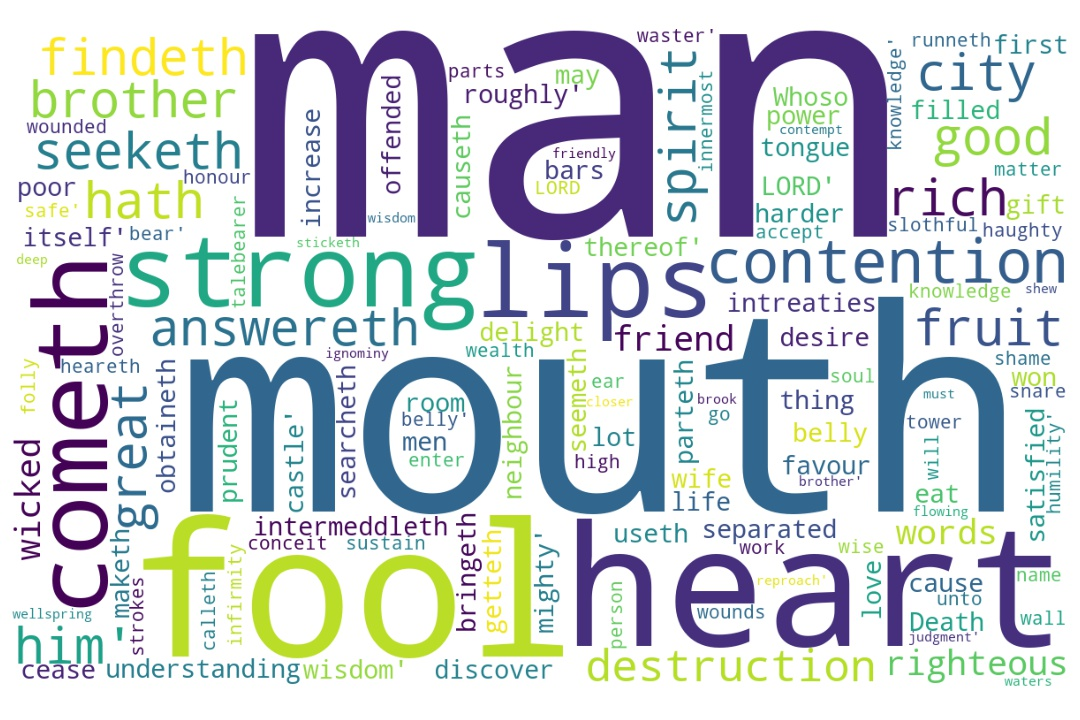
\includegraphics[width=\linewidth]{20OT-Proverbs/Proverb18-WordCloud.jpg}
  \caption{Proverb 18 Word Cloud}
  \label{fig:Proverb 18 word Cloud}
\end{figure}

\marginpar{\scriptsize \centering \fcolorbox{bone}{lime}{\textbf{A MAN FOCUSED ON GOD}}\\ (Proverbs 18:1-24) \begin{compactenum}[I.][8]
    \item Will be an \textbf{Inspired Man} - 
    \item Will be \textbf{Separate from the Ignorant Masses} - 
    \item For him most things in life will have  
    \textbf{Insignificant Meaning} - 
    \item Lives in an \textbf{Isolated Manner} 
    \item Lives by an \textbf{Individual Mandate} 
    \item Has an \textbf{intense and Insular Mentality}
\end{compactenum}}

\marginpar{\scriptsize \centering \fcolorbox{bone}{yellow}{\textbf{A FRIEND LIKE JESUS}}\\ (Proverb 18:24) \begin{compactenum}[I.][8]
    \item A \textbf{Close} Friend
    \item A \textbf{Constant} Friend
    \item A \textbf{Confiding} Friend
    \item A \textbf{Concerned} Friend
    \item A \textbf{Continuing} Friend
    \item A \textbf{Capable} Friend
    \item A \textbf{Caring} Friend
\end{compactenum}}

\marginpar{\scriptsize \centering \fcolorbox{bone}{black}{\textbf{\textcolor{white}{THE PURSUIT OF WISDOM}}}\\ (Proverb 18:24) \begin{compactenum}[I.][8]
    \item Then \textbf{Perverted} Motive -- to learn how manipulate events and circumstances. \index[scripture]{Proverbs!Pro 18:01}(Proverb 18:1)
    \item Then \textbf{Prideful} Motive -- To become exalted as wise. 
    \item Then \textbf{Public} Motive -- to be known and famous. 
    \item Then \textbf{Personal} Motive -- to achieve understanding. 
    \item Then \textbf{Practical} Motive -- to learn how live without mistakes or errors. 
    \item Then \textbf{Purposeful} Motive -- to learn navigate a specific problem. 
    \item Then \textbf{Perfect} Motive -- to learn how to live righteously before God. 
\end{compactenum}}

\marginpar{\scriptsize \centering \fcolorbox{bone}{blue}{\textbf{\textcolor{white}{WHAT YOUR SPEECH REVEALS}}}\\ (Proverb 18:4) \begin{compactenum}[I.][8]
    \item \textbf{Your Education} 
    \item \textbf{Your Excellence} 
    \item \textbf{Your Excitements} 
    \item \textbf{Your Enmity} 
    \item \textbf{Your Enemies} 
    \item \textbf{Your End} 
    \item \textbf{Your Emptiness}
    \item \textbf{Your Entanglements} 
\end{compactenum} }

\marginpar{\scriptsize \centering \fcolorbox{bone}{orange}{\textbf{THE WISE MAN}}\\ (Proverbs 18:1-24) \begin{compactenum}[I.][8]
    \item \textbf{Is Distinctive}
    \item \textbf{Is Disciplined}
    \item \textbf{Ignores Distractions}
    \item \textbf{Finds Delights in Wisdom}
    \item \textbf{Has Departed from the Common and Mundane}
    \item \textbf{Has a Distaste for Foolishness}
    \item \textbf{Is often regarded as Disturbed}
\end{compactenum} }




\footnote{\textcolor[cmyk]{0.99998,1,0,0}{\hyperlink{TOC}{Return to end of Table of Contents.}}}\footnote{\href{https://audiobible.com/bible/proverbs_18.html}{\textcolor[cmyk]{0.99998,1,0,0}{Proverbs Audio}}}\textcolor[cmyk]{0.99998,1,0,0}{Through desire a man, having separated himself, seeketh \emph{and} \fcolorbox{bone}{MYGOLD}{intermeddleth} with all wisdom.}
[2] \textcolor[cmyk]{0.99998,1,0,0}{A fool hath no delight in \fcolorbox{bone}{MYGOLD}{understanding}, but that \fcolorbox{bone}{bone}{his} heart may discover itself.}
[3] \textcolor[cmyk]{0.99998,1,0,0}{When the wicked cometh, \emph{then} cometh also contempt, and with ignominy reproach.}
[4] \textcolor[cmyk]{0.99998,1,0,0}{The words of a man's mouth \emph{are} \emph{as} deep waters, \emph{and} the wellspring of wisdom \emph{as} a flowing brook.}\footnote{\textbf{Proverb 16:22} - Understanding is a wellspring of life unto him that hath it: but the instruction of fools is folly.}
[5] \textcolor[cmyk]{0.99998,1,0,0}{\emph{It} \emph{is} not good to accept the person of the wicked, to overthrow the righteous in judgment.}
[6] \textcolor[cmyk]{0.99998,1,0,0}{A fool's lips enter into contention, and \fcolorbox{bone}{bone}{his} mouth calleth for strokes.}
[7] \textcolor[cmyk]{0.99998,1,0,0}{A fool's mouth \emph{is} \fcolorbox{bone}{bone}{his} destruction, and \fcolorbox{bone}{bone}{his} lips \emph{are} the snare of \fcolorbox{bone}{bone}{his} soul.}
[8] \textcolor[cmyk]{0.99998,1,0,0}{The words of a talebearer \emph{are} as wounds, and they go down into the innermost parts of the belly.}
[9] \textcolor[cmyk]{0.99998,1,0,0}{He also that is slothful in \fcolorbox{bone}{bone}{his} work is brother to him that is a great waster.}
[10] \textcolor[cmyk]{0.99998,1,0,0}{The name of the LORD \emph{is} a strong tower: the righteous runneth into it, and is safe.}
[11] \textcolor[cmyk]{0.99998,1,0,0}{The rich man's wealth \emph{is} \fcolorbox{bone}{bone}{his} strong city, and as an high wall in \fcolorbox{bone}{bone}{his} own conceit.}
[12] \textcolor[cmyk]{0.99998,1,0,0}{Before destruction the heart of man is haughty, and before honour \emph{is} humility.}
[13] \textcolor[cmyk]{0.99998,1,0,0}{He that answereth a matter before he heareth \emph{it}, it \emph{is} folly and shame unto him.}
[14] \textcolor[cmyk]{0.99998,1,0,0}{The spirit of a man will sustain \fcolorbox{bone}{bone}{his} infirmity; but a wounded spirit who can bear?}
[15] \textcolor[cmyk]{0.99998,1,0,0}{The heart of the prudent getteth knowledge; and the ear of the wise seeketh knowledge.}
[16] \textcolor[cmyk]{0.99998,1,0,0}{A man's gift maketh room for him, and bringeth him before great men.}
[17] \textcolor[cmyk]{0.99998,1,0,0}{\emph{He} \emph{that} \emph{is} first in \fcolorbox{bone}{bone}{his} own cause \emph{seemeth} just; but \fcolorbox{bone}{bone}{his} neighbour cometh and searcheth him.}
[18] \textcolor[cmyk]{0.99998,1,0,0}{The lot causeth contentions to cease, and parteth between the mighty.}
[19] \textcolor[cmyk]{0.99998,1,0,0}{A brother offended \emph{is} \emph{harder} \emph{to} \emph{be} \emph{won} than a strong city: and \emph{their} contentions \emph{are} like the bars of a castle.}
[20] \textcolor[cmyk]{0.99998,1,0,0}{A man's belly shall be satisfied with the fruit of \fcolorbox{bone}{bone}{his} mouth; \emph{and} with the increase of \fcolorbox{bone}{bone}{his} lips shall he be filled.}
[21] \textcolor[cmyk]{0.99998,1,0,0}{Death and life \emph{are} in the power of the tongue: and they that love it shall eat the fruit thereof.}
[22] \textcolor[cmyk]{0.99998,1,0,0}{\emph{Whoso} findeth a wife findeth a good \emph{thing}, and obtaineth favour of the LORD.}
[23] \textcolor[cmyk]{0.99998,1,0,0}{The poor useth intreaties; but the rich answereth roughly.}
[24] \textcolor[cmyk]{0.99998,1,0,0}{A man \emph{that} \emph{hath} friends must shew himself friendly: and there is a friend \emph{that} sticketh closer than a brother.}



\index[NWIV]{13!Proverbs!Pro 18:1}\index[AWIP]{Through!Proverbs!Pro 18:1}\index[AWIP]{desire!Proverbs!Pro 18:1}\index[AWIP]{a!Proverbs!Pro 18:1}\index[AWIP]{man!Proverbs!Pro 18:1}\index[AWIP]{having!Proverbs!Pro 18:1}\index[AWIP]{separated!Proverbs!Pro 18:1}\index[AWIP]{himself!Proverbs!Pro 18:1}\index[AWIP]{seeketh!Proverbs!Pro 18:1}\index[AWIP]{\emph{and}!Proverbs!Pro 18:1}\index[AWIP]{intermeddleth!Proverbs!Pro 18:1}\index[AWIP]{with!Proverbs!Pro 18:1}\index[AWIP]{all!Proverbs!Pro 18:1}\index[AWIP]{wisdom!Proverbs!Pro 18:1}\index[AWIP]{\emph{and}!Proverbs!Pro 18:1}

\index[NWIV]{14!Proverbs!Pro 18:2}\index[AWIP]{A!Proverbs!Pro 18:2}\index[AWIP]{fool!Proverbs!Pro 18:2}\index[AWIP]{hath!Proverbs!Pro 18:2}\index[AWIP]{no!Proverbs!Pro 18:2}\index[AWIP]{delight!Proverbs!Pro 18:2}\index[AWIP]{in!Proverbs!Pro 18:2}\index[AWIP]{understanding!Proverbs!Pro 18:2}\index[AWIP]{but!Proverbs!Pro 18:2}\index[AWIP]{that!Proverbs!Pro 18:2}\index[AWIP]{his!Proverbs!Pro 18:2}\index[AWIP]{heart!Proverbs!Pro 18:2}\index[AWIP]{may!Proverbs!Pro 18:2}\index[AWIP]{discover!Proverbs!Pro 18:2}\index[AWIP]{itself!Proverbs!Pro 18:2}

\index[NWIV]{12!Proverbs!Pro 18:3}\index[AWIP]{When!Proverbs!Pro 18:3}\index[AWIP]{the!Proverbs!Pro 18:3}\index[AWIP]{wicked!Proverbs!Pro 18:3}\index[AWIP]{cometh!Proverbs!Pro 18:3}\index[AWIP]{cometh!Proverbs!Pro 18:3 (2)}\index[AWIP]{\emph{then}!Proverbs!Pro 18:3}\index[AWIP]{also!Proverbs!Pro 18:3}\index[AWIP]{contempt!Proverbs!Pro 18:3}\index[AWIP]{and!Proverbs!Pro 18:3}\index[AWIP]{with!Proverbs!Pro 18:3}\index[AWIP]{ignominy!Proverbs!Pro 18:3}\index[AWIP]{reproach!Proverbs!Pro 18:3}\index[AWIP]{\emph{then}!Proverbs!Pro 18:3}

\index[NWIV]{19!Proverbs!Pro 18:4}\index[AWIP]{The!Proverbs!Pro 18:4}\index[AWIP]{words!Proverbs!Pro 18:4}\index[AWIP]{of!Proverbs!Pro 18:4}\index[AWIP]{of!Proverbs!Pro 18:4 (2)}\index[AWIP]{a!Proverbs!Pro 18:4}\index[AWIP]{a!Proverbs!Pro 18:4 (2)}\index[AWIP]{man's!Proverbs!Pro 18:4}\index[AWIP]{mouth!Proverbs!Pro 18:4}\index[AWIP]{\emph{are}!Proverbs!Pro 18:4}\index[AWIP]{\emph{as}!Proverbs!Pro 18:4}\index[AWIP]{\emph{as}!Proverbs!Pro 18:4 (2)}\index[AWIP]{deep!Proverbs!Pro 18:4}\index[AWIP]{waters!Proverbs!Pro 18:4}\index[AWIP]{\emph{and}!Proverbs!Pro 18:4}\index[AWIP]{the!Proverbs!Pro 18:4}\index[AWIP]{wellspring!Proverbs!Pro 18:4}\index[AWIP]{wisdom!Proverbs!Pro 18:4}\index[AWIP]{flowing!Proverbs!Pro 18:4}\index[AWIP]{brook!Proverbs!Pro 18:4}\index[AWIP]{\emph{are}!Proverbs!Pro 18:4}\index[AWIP]{\emph{as}!Proverbs!Pro 18:4}\index[AWIP]{\emph{as}!Proverbs!Pro 18:4 (2)}\index[AWIP]{\emph{and}!Proverbs!Pro 18:4}

\index[NWIV]{17!Proverbs!Pro 18:5}\index[AWIP]{\emph{It}!Proverbs!Pro 18:5}\index[AWIP]{\emph{is}!Proverbs!Pro 18:5}\index[AWIP]{not!Proverbs!Pro 18:5}\index[AWIP]{good!Proverbs!Pro 18:5}\index[AWIP]{to!Proverbs!Pro 18:5}\index[AWIP]{to!Proverbs!Pro 18:5 (2)}\index[AWIP]{accept!Proverbs!Pro 18:5}\index[AWIP]{the!Proverbs!Pro 18:5}\index[AWIP]{the!Proverbs!Pro 18:5 (2)}\index[AWIP]{the!Proverbs!Pro 18:5 (3)}\index[AWIP]{person!Proverbs!Pro 18:5}\index[AWIP]{of!Proverbs!Pro 18:5}\index[AWIP]{wicked!Proverbs!Pro 18:5}\index[AWIP]{overthrow!Proverbs!Pro 18:5}\index[AWIP]{righteous!Proverbs!Pro 18:5}\index[AWIP]{in!Proverbs!Pro 18:5}\index[AWIP]{judgment!Proverbs!Pro 18:5}\index[AWIP]{\emph{It}!Proverbs!Pro 18:5}\index[AWIP]{\emph{is}!Proverbs!Pro 18:5}

\index[NWIV]{12!Proverbs!Pro 18:6}\index[AWIP]{A!Proverbs!Pro 18:6}\index[AWIP]{fool's!Proverbs!Pro 18:6}\index[AWIP]{lips!Proverbs!Pro 18:6}\index[AWIP]{enter!Proverbs!Pro 18:6}\index[AWIP]{into!Proverbs!Pro 18:6}\index[AWIP]{contention!Proverbs!Pro 18:6}\index[AWIP]{and!Proverbs!Pro 18:6}\index[AWIP]{his!Proverbs!Pro 18:6}\index[AWIP]{mouth!Proverbs!Pro 18:6}\index[AWIP]{calleth!Proverbs!Pro 18:6}\index[AWIP]{for!Proverbs!Pro 18:6}\index[AWIP]{strokes!Proverbs!Pro 18:6}

\index[NWIV]{15!Proverbs!Pro 18:7}\index[AWIP]{A!Proverbs!Pro 18:7}\index[AWIP]{fool's!Proverbs!Pro 18:7}\index[AWIP]{mouth!Proverbs!Pro 18:7}\index[AWIP]{\emph{is}!Proverbs!Pro 18:7}\index[AWIP]{his!Proverbs!Pro 18:7}\index[AWIP]{his!Proverbs!Pro 18:7 (2)}\index[AWIP]{his!Proverbs!Pro 18:7 (3)}\index[AWIP]{destruction!Proverbs!Pro 18:7}\index[AWIP]{and!Proverbs!Pro 18:7}\index[AWIP]{lips!Proverbs!Pro 18:7}\index[AWIP]{\emph{are}!Proverbs!Pro 18:7}\index[AWIP]{the!Proverbs!Pro 18:7}\index[AWIP]{snare!Proverbs!Pro 18:7}\index[AWIP]{of!Proverbs!Pro 18:7}\index[AWIP]{soul!Proverbs!Pro 18:7}\index[AWIP]{\emph{is}!Proverbs!Pro 18:7}\index[AWIP]{\emph{are}!Proverbs!Pro 18:7}

\index[NWIV]{19!Proverbs!Pro 18:8}\index[AWIP]{The!Proverbs!Pro 18:8}\index[AWIP]{words!Proverbs!Pro 18:8}\index[AWIP]{of!Proverbs!Pro 18:8}\index[AWIP]{of!Proverbs!Pro 18:8 (2)}\index[AWIP]{a!Proverbs!Pro 18:8}\index[AWIP]{talebearer!Proverbs!Pro 18:8}\index[AWIP]{\emph{are}!Proverbs!Pro 18:8}\index[AWIP]{as!Proverbs!Pro 18:8}\index[AWIP]{wounds!Proverbs!Pro 18:8}\index[AWIP]{and!Proverbs!Pro 18:8}\index[AWIP]{they!Proverbs!Pro 18:8}\index[AWIP]{go!Proverbs!Pro 18:8}\index[AWIP]{down!Proverbs!Pro 18:8}\index[AWIP]{into!Proverbs!Pro 18:8}\index[AWIP]{the!Proverbs!Pro 18:8}\index[AWIP]{the!Proverbs!Pro 18:8 (2)}\index[AWIP]{innermost!Proverbs!Pro 18:8}\index[AWIP]{parts!Proverbs!Pro 18:8}\index[AWIP]{belly!Proverbs!Pro 18:8}\index[AWIP]{\emph{are}!Proverbs!Pro 18:8}

\index[NWIV]{17!Proverbs!Pro 18:9}\index[AWIP]{He!Proverbs!Pro 18:9}\index[AWIP]{also!Proverbs!Pro 18:9}\index[AWIP]{that!Proverbs!Pro 18:9}\index[AWIP]{that!Proverbs!Pro 18:9 (2)}\index[AWIP]{is!Proverbs!Pro 18:9}\index[AWIP]{is!Proverbs!Pro 18:9 (2)}\index[AWIP]{is!Proverbs!Pro 18:9 (3)}\index[AWIP]{slothful!Proverbs!Pro 18:9}\index[AWIP]{in!Proverbs!Pro 18:9}\index[AWIP]{his!Proverbs!Pro 18:9}\index[AWIP]{work!Proverbs!Pro 18:9}\index[AWIP]{brother!Proverbs!Pro 18:9}\index[AWIP]{to!Proverbs!Pro 18:9}\index[AWIP]{him!Proverbs!Pro 18:9}\index[AWIP]{a!Proverbs!Pro 18:9}\index[AWIP]{great!Proverbs!Pro 18:9}\index[AWIP]{waster!Proverbs!Pro 18:9}

\index[NWIV]{17!Proverbs!Pro 18:10}\index[AWIP]{The!Proverbs!Pro 18:10}\index[AWIP]{name!Proverbs!Pro 18:10}\index[AWIP]{of!Proverbs!Pro 18:10}\index[AWIP]{the!Proverbs!Pro 18:10}\index[AWIP]{the!Proverbs!Pro 18:10 (2)}\index[AWIP]{LORD!Proverbs!Pro 18:10}\index[AWIP]{\emph{is}!Proverbs!Pro 18:10}\index[AWIP]{a!Proverbs!Pro 18:10}\index[AWIP]{strong!Proverbs!Pro 18:10}\index[AWIP]{tower!Proverbs!Pro 18:10}\index[AWIP]{righteous!Proverbs!Pro 18:10}\index[AWIP]{runneth!Proverbs!Pro 18:10}\index[AWIP]{into!Proverbs!Pro 18:10}\index[AWIP]{it!Proverbs!Pro 18:10}\index[AWIP]{and!Proverbs!Pro 18:10}\index[AWIP]{is!Proverbs!Pro 18:10}\index[AWIP]{safe!Proverbs!Pro 18:10}\index[AWIP]{\emph{is}!Proverbs!Pro 18:10}

\index[NWIV]{17!Proverbs!Pro 18:11}\index[AWIP]{The!Proverbs!Pro 18:11}\index[AWIP]{rich!Proverbs!Pro 18:11}\index[AWIP]{man's!Proverbs!Pro 18:11}\index[AWIP]{wealth!Proverbs!Pro 18:11}\index[AWIP]{\emph{is}!Proverbs!Pro 18:11}\index[AWIP]{his!Proverbs!Pro 18:11}\index[AWIP]{his!Proverbs!Pro 18:11 (2)}\index[AWIP]{strong!Proverbs!Pro 18:11}\index[AWIP]{city!Proverbs!Pro 18:11}\index[AWIP]{and!Proverbs!Pro 18:11}\index[AWIP]{as!Proverbs!Pro 18:11}\index[AWIP]{an!Proverbs!Pro 18:11}\index[AWIP]{high!Proverbs!Pro 18:11}\index[AWIP]{wall!Proverbs!Pro 18:11}\index[AWIP]{in!Proverbs!Pro 18:11}\index[AWIP]{own!Proverbs!Pro 18:11}\index[AWIP]{conceit!Proverbs!Pro 18:11}\index[AWIP]{\emph{is}!Proverbs!Pro 18:11}

\index[NWIV]{13!Proverbs!Pro 18:12}\index[AWIP]{Before!Proverbs!Pro 18:12}\index[AWIP]{destruction!Proverbs!Pro 18:12}\index[AWIP]{the!Proverbs!Pro 18:12}\index[AWIP]{heart!Proverbs!Pro 18:12}\index[AWIP]{of!Proverbs!Pro 18:12}\index[AWIP]{man!Proverbs!Pro 18:12}\index[AWIP]{is!Proverbs!Pro 18:12}\index[AWIP]{haughty!Proverbs!Pro 18:12}\index[AWIP]{and!Proverbs!Pro 18:12}\index[AWIP]{before!Proverbs!Pro 18:12}\index[AWIP]{honour!Proverbs!Pro 18:12}\index[AWIP]{\emph{is}!Proverbs!Pro 18:12}\index[AWIP]{humility!Proverbs!Pro 18:12}\index[AWIP]{\emph{is}!Proverbs!Pro 18:12}

\index[NWIV]{16!Proverbs!Pro 18:13}\index[AWIP]{He!Proverbs!Pro 18:13}\index[AWIP]{that!Proverbs!Pro 18:13}\index[AWIP]{answereth!Proverbs!Pro 18:13}\index[AWIP]{a!Proverbs!Pro 18:13}\index[AWIP]{matter!Proverbs!Pro 18:13}\index[AWIP]{before!Proverbs!Pro 18:13}\index[AWIP]{he!Proverbs!Pro 18:13}\index[AWIP]{heareth!Proverbs!Pro 18:13}\index[AWIP]{\emph{it}!Proverbs!Pro 18:13}\index[AWIP]{it!Proverbs!Pro 18:13}\index[AWIP]{\emph{is}!Proverbs!Pro 18:13}\index[AWIP]{folly!Proverbs!Pro 18:13}\index[AWIP]{and!Proverbs!Pro 18:13}\index[AWIP]{shame!Proverbs!Pro 18:13}\index[AWIP]{unto!Proverbs!Pro 18:13}\index[AWIP]{him!Proverbs!Pro 18:13}\index[AWIP]{\emph{it}!Proverbs!Pro 18:13}\index[AWIP]{\emph{is}!Proverbs!Pro 18:13}

\index[NWIV]{16!Proverbs!Pro 18:14}\index[AWIP]{The!Proverbs!Pro 18:14}\index[AWIP]{spirit!Proverbs!Pro 18:14}\index[AWIP]{spirit!Proverbs!Pro 18:14 (2)}\index[AWIP]{of!Proverbs!Pro 18:14}\index[AWIP]{a!Proverbs!Pro 18:14}\index[AWIP]{a!Proverbs!Pro 18:14 (2)}\index[AWIP]{man!Proverbs!Pro 18:14}\index[AWIP]{will!Proverbs!Pro 18:14}\index[AWIP]{sustain!Proverbs!Pro 18:14}\index[AWIP]{his!Proverbs!Pro 18:14}\index[AWIP]{infirmity!Proverbs!Pro 18:14}\index[AWIP]{but!Proverbs!Pro 18:14}\index[AWIP]{wounded!Proverbs!Pro 18:14}\index[AWIP]{who!Proverbs!Pro 18:14}\index[AWIP]{can!Proverbs!Pro 18:14}\index[AWIP]{bear?!Proverbs!Pro 18:14}

\index[NWIV]{15!Proverbs!Pro 18:15}\index[AWIP]{The!Proverbs!Pro 18:15}\index[AWIP]{heart!Proverbs!Pro 18:15}\index[AWIP]{of!Proverbs!Pro 18:15}\index[AWIP]{of!Proverbs!Pro 18:15 (2)}\index[AWIP]{the!Proverbs!Pro 18:15}\index[AWIP]{the!Proverbs!Pro 18:15 (2)}\index[AWIP]{the!Proverbs!Pro 18:15 (3)}\index[AWIP]{prudent!Proverbs!Pro 18:15}\index[AWIP]{getteth!Proverbs!Pro 18:15}\index[AWIP]{knowledge!Proverbs!Pro 18:15}\index[AWIP]{knowledge!Proverbs!Pro 18:15 (2)}\index[AWIP]{and!Proverbs!Pro 18:15}\index[AWIP]{ear!Proverbs!Pro 18:15}\index[AWIP]{wise!Proverbs!Pro 18:15}\index[AWIP]{seeketh!Proverbs!Pro 18:15}

\index[NWIV]{13!Proverbs!Pro 18:16}\index[AWIP]{A!Proverbs!Pro 18:16}\index[AWIP]{man's!Proverbs!Pro 18:16}\index[AWIP]{gift!Proverbs!Pro 18:16}\index[AWIP]{maketh!Proverbs!Pro 18:16}\index[AWIP]{room!Proverbs!Pro 18:16}\index[AWIP]{for!Proverbs!Pro 18:16}\index[AWIP]{him!Proverbs!Pro 18:16}\index[AWIP]{him!Proverbs!Pro 18:16 (2)}\index[AWIP]{and!Proverbs!Pro 18:16}\index[AWIP]{bringeth!Proverbs!Pro 18:16}\index[AWIP]{before!Proverbs!Pro 18:16}\index[AWIP]{great!Proverbs!Pro 18:16}\index[AWIP]{men!Proverbs!Pro 18:16}

\index[NWIV]{17!Proverbs!Pro 18:17}\index[AWIP]{\emph{He}!Proverbs!Pro 18:17}\index[AWIP]{\emph{that}!Proverbs!Pro 18:17}\index[AWIP]{\emph{is}!Proverbs!Pro 18:17}\index[AWIP]{first!Proverbs!Pro 18:17}\index[AWIP]{in!Proverbs!Pro 18:17}\index[AWIP]{his!Proverbs!Pro 18:17}\index[AWIP]{his!Proverbs!Pro 18:17 (2)}\index[AWIP]{own!Proverbs!Pro 18:17}\index[AWIP]{cause!Proverbs!Pro 18:17}\index[AWIP]{\emph{seemeth}!Proverbs!Pro 18:17}\index[AWIP]{just!Proverbs!Pro 18:17}\index[AWIP]{but!Proverbs!Pro 18:17}\index[AWIP]{neighbour!Proverbs!Pro 18:17}\index[AWIP]{cometh!Proverbs!Pro 18:17}\index[AWIP]{and!Proverbs!Pro 18:17}\index[AWIP]{searcheth!Proverbs!Pro 18:17}\index[AWIP]{him!Proverbs!Pro 18:17}\index[AWIP]{\emph{He}!Proverbs!Pro 18:17}\index[AWIP]{\emph{that}!Proverbs!Pro 18:17}\index[AWIP]{\emph{is}!Proverbs!Pro 18:17}\index[AWIP]{\emph{seemeth}!Proverbs!Pro 18:17}

\index[NWIV]{11!Proverbs!Pro 18:18}\index[AWIP]{The!Proverbs!Pro 18:18}\index[AWIP]{lot!Proverbs!Pro 18:18}\index[AWIP]{causeth!Proverbs!Pro 18:18}\index[AWIP]{contentions!Proverbs!Pro 18:18}\index[AWIP]{to!Proverbs!Pro 18:18}\index[AWIP]{cease!Proverbs!Pro 18:18}\index[AWIP]{and!Proverbs!Pro 18:18}\index[AWIP]{parteth!Proverbs!Pro 18:18}\index[AWIP]{between!Proverbs!Pro 18:18}\index[AWIP]{the!Proverbs!Pro 18:18}\index[AWIP]{mighty!Proverbs!Pro 18:18}

\index[NWIV]{22!Proverbs!Pro 18:19}\index[AWIP]{A!Proverbs!Pro 18:19}\index[AWIP]{brother!Proverbs!Pro 18:19}\index[AWIP]{offended!Proverbs!Pro 18:19}\index[AWIP]{\emph{is}!Proverbs!Pro 18:19}\index[AWIP]{\emph{harder}!Proverbs!Pro 18:19}\index[AWIP]{\emph{to}!Proverbs!Pro 18:19}\index[AWIP]{\emph{be}!Proverbs!Pro 18:19}\index[AWIP]{\emph{won}!Proverbs!Pro 18:19}\index[AWIP]{than!Proverbs!Pro 18:19}\index[AWIP]{a!Proverbs!Pro 18:19}\index[AWIP]{a!Proverbs!Pro 18:19 (2)}\index[AWIP]{strong!Proverbs!Pro 18:19}\index[AWIP]{city!Proverbs!Pro 18:19}\index[AWIP]{and!Proverbs!Pro 18:19}\index[AWIP]{\emph{their}!Proverbs!Pro 18:19}\index[AWIP]{contentions!Proverbs!Pro 18:19}\index[AWIP]{\emph{are}!Proverbs!Pro 18:19}\index[AWIP]{like!Proverbs!Pro 18:19}\index[AWIP]{the!Proverbs!Pro 18:19}\index[AWIP]{bars!Proverbs!Pro 18:19}\index[AWIP]{of!Proverbs!Pro 18:19}\index[AWIP]{castle!Proverbs!Pro 18:19}\index[AWIP]{\emph{is}!Proverbs!Pro 18:19}\index[AWIP]{\emph{harder}!Proverbs!Pro 18:19}\index[AWIP]{\emph{to}!Proverbs!Pro 18:19}\index[AWIP]{\emph{be}!Proverbs!Pro 18:19}\index[AWIP]{\emph{won}!Proverbs!Pro 18:19}\index[AWIP]{\emph{their}!Proverbs!Pro 18:19}\index[AWIP]{\emph{are}!Proverbs!Pro 18:19}

\index[NWIV]{23!Proverbs!Pro 18:20}\index[AWIP]{A!Proverbs!Pro 18:20}\index[AWIP]{man's!Proverbs!Pro 18:20}\index[AWIP]{belly!Proverbs!Pro 18:20}\index[AWIP]{shall!Proverbs!Pro 18:20}\index[AWIP]{shall!Proverbs!Pro 18:20 (2)}\index[AWIP]{be!Proverbs!Pro 18:20}\index[AWIP]{be!Proverbs!Pro 18:20 (2)}\index[AWIP]{satisfied!Proverbs!Pro 18:20}\index[AWIP]{with!Proverbs!Pro 18:20}\index[AWIP]{with!Proverbs!Pro 18:20 (2)}\index[AWIP]{the!Proverbs!Pro 18:20}\index[AWIP]{the!Proverbs!Pro 18:20 (2)}\index[AWIP]{fruit!Proverbs!Pro 18:20}\index[AWIP]{of!Proverbs!Pro 18:20}\index[AWIP]{of!Proverbs!Pro 18:20 (2)}\index[AWIP]{his!Proverbs!Pro 18:20}\index[AWIP]{his!Proverbs!Pro 18:20 (2)}\index[AWIP]{mouth!Proverbs!Pro 18:20}\index[AWIP]{\emph{and}!Proverbs!Pro 18:20}\index[AWIP]{increase!Proverbs!Pro 18:20}\index[AWIP]{lips!Proverbs!Pro 18:20}\index[AWIP]{he!Proverbs!Pro 18:20}\index[AWIP]{filled!Proverbs!Pro 18:20}\index[AWIP]{\emph{and}!Proverbs!Pro 18:20}

\index[NWIV]{20!Proverbs!Pro 18:21}\index[AWIP]{Death!Proverbs!Pro 18:21}\index[AWIP]{and!Proverbs!Pro 18:21}\index[AWIP]{and!Proverbs!Pro 18:21 (2)}\index[AWIP]{life!Proverbs!Pro 18:21}\index[AWIP]{\emph{are}!Proverbs!Pro 18:21}\index[AWIP]{in!Proverbs!Pro 18:21}\index[AWIP]{the!Proverbs!Pro 18:21}\index[AWIP]{the!Proverbs!Pro 18:21 (2)}\index[AWIP]{the!Proverbs!Pro 18:21 (3)}\index[AWIP]{power!Proverbs!Pro 18:21}\index[AWIP]{of!Proverbs!Pro 18:21}\index[AWIP]{tongue!Proverbs!Pro 18:21}\index[AWIP]{they!Proverbs!Pro 18:21}\index[AWIP]{that!Proverbs!Pro 18:21}\index[AWIP]{love!Proverbs!Pro 18:21}\index[AWIP]{it!Proverbs!Pro 18:21}\index[AWIP]{shall!Proverbs!Pro 18:21}\index[AWIP]{eat!Proverbs!Pro 18:21}\index[AWIP]{fruit!Proverbs!Pro 18:21}\index[AWIP]{thereof!Proverbs!Pro 18:21}\index[AWIP]{\emph{are}!Proverbs!Pro 18:21}

\index[NWIV]{14!Proverbs!Pro 18:22}\index[AWIP]{\emph{Whoso}!Proverbs!Pro 18:22}\index[AWIP]{findeth!Proverbs!Pro 18:22}\index[AWIP]{findeth!Proverbs!Pro 18:22 (2)}\index[AWIP]{a!Proverbs!Pro 18:22}\index[AWIP]{a!Proverbs!Pro 18:22 (2)}\index[AWIP]{wife!Proverbs!Pro 18:22}\index[AWIP]{good!Proverbs!Pro 18:22}\index[AWIP]{\emph{thing}!Proverbs!Pro 18:22}\index[AWIP]{and!Proverbs!Pro 18:22}\index[AWIP]{obtaineth!Proverbs!Pro 18:22}\index[AWIP]{favour!Proverbs!Pro 18:22}\index[AWIP]{of!Proverbs!Pro 18:22}\index[AWIP]{the!Proverbs!Pro 18:22}\index[AWIP]{LORD!Proverbs!Pro 18:22}\index[AWIP]{\emph{Whoso}!Proverbs!Pro 18:22}\index[AWIP]{\emph{thing}!Proverbs!Pro 18:22}

\index[NWIV]{9!Proverbs!Pro 18:23}\index[AWIP]{The!Proverbs!Pro 18:23}\index[AWIP]{poor!Proverbs!Pro 18:23}\index[AWIP]{useth!Proverbs!Pro 18:23}\index[AWIP]{intreaties!Proverbs!Pro 18:23}\index[AWIP]{but!Proverbs!Pro 18:23}\index[AWIP]{the!Proverbs!Pro 18:23}\index[AWIP]{rich!Proverbs!Pro 18:23}\index[AWIP]{answereth!Proverbs!Pro 18:23}\index[AWIP]{roughly!Proverbs!Pro 18:23}

\index[NWIV]{20!Proverbs!Pro 18:24}\index[AWIP]{A!Proverbs!Pro 18:24}\index[AWIP]{man!Proverbs!Pro 18:24}\index[AWIP]{\emph{that}!Proverbs!Pro 18:24}\index[AWIP]{\emph{that}!Proverbs!Pro 18:24 (2)}\index[AWIP]{\emph{hath}!Proverbs!Pro 18:24}\index[AWIP]{friends!Proverbs!Pro 18:24}\index[AWIP]{must!Proverbs!Pro 18:24}\index[AWIP]{shew!Proverbs!Pro 18:24}\index[AWIP]{himself!Proverbs!Pro 18:24}\index[AWIP]{friendly!Proverbs!Pro 18:24}\index[AWIP]{and!Proverbs!Pro 18:24}\index[AWIP]{there!Proverbs!Pro 18:24}\index[AWIP]{is!Proverbs!Pro 18:24}\index[AWIP]{a!Proverbs!Pro 18:24}\index[AWIP]{a!Proverbs!Pro 18:24 (2)}\index[AWIP]{friend!Proverbs!Pro 18:24}\index[AWIP]{sticketh!Proverbs!Pro 18:24}\index[AWIP]{closer!Proverbs!Pro 18:24}\index[AWIP]{than!Proverbs!Pro 18:24}\index[AWIP]{brother!Proverbs!Pro 18:24}\index[AWIP]{\emph{that}!Proverbs!Pro 18:24}\index[AWIP]{\emph{that}!Proverbs!Pro 18:24 (2)}\index[AWIP]{\emph{hath}!Proverbs!Pro 18:24}


\section{Proverb 18 Outlines}

\subsection{My Outlines}

\subsubsection{A Man Focused on God's Wisdom}
\index[speaker]{Keith Anthony!Proverb 18 (A Man Focused on God's Wisdom)}
\index[series]{Proverbs (Keith Anthony)!Pro 18 (A Man Focused on God's Wisdom)}
\index[date]{2014/11/18!Proverb 18 (A Man Focused on God's Wisdom) (Keith Anthony)}
Proverbs 18:1 gives some hints about a man who is ostensibly focused on getting God's wisdom. Can we relate to this kind of person? Do we have any biblical examples? Could it be Elijah, or John the Baptist?
\begin{compactenum}[I.]
    \item Will be an \textbf{Inspired Man} - 
    \item Will be \textbf{Separate from the Ignorant Masses} - 
    \item For him most things in life will have  \textbf{Insignificant Meaning} - 
    \item Lives in an \textbf{Isolated Manner} 
    \item Lives by an \textbf{Individual Mandate} -  seldom supported by friends, and 
    \item Has an \textbf{intense and Insular Mentality} - 
\end{compactenum}
So, this is a guy who is mostly unwanted and unwelcome. Vast majority cannot related to him. How much are you like this man? How much do you want to be? How much do you think you should be?

\subsubsection{A Friend Like Jesus}
\index[speaker]{Keith Anthony!Proverb 18 (A Friend Like Jesus)}
\index[series]{Proverbs (Keith Anthony)!Pro 18 (A Friend Like Jesus)}
\index[date]{2014/11/18!Proverb 18 (A Friend Like Jesus (Keith Anthony)}
\begin{compactenum}[I.][8]
    \item A \textbf{Close} Friend
    \item A \textbf{Constant} Friend
    \item A \textbf{Confiding} Friend
    \item A \textbf{Concerned} Friend
    \item A \textbf{Continuing} Friend
    \item A \textbf{Capable} Friend
    \item A \textbf{Caring} Friend
\end{compactenum}


\subsubsection{The Pursuit of Wisdom}
\index[speaker]{Keith Anthony!Proverb 18 (The Pursuit of Wisdom)}
\index[series]{Proverbs (Keith Anthony)!Pro 18 (The Pursuit of Wisdom)}
\index[date]{2017/03/18!Proverb 18:01 (The Pursuit of Wisdom) (Keith Anthony)}
At issue in the pursuit of wisdom, is the underlying heart motive. I contest that ``Wisdom'' is not a thing, but a person, an individual, who is reading our motives as we go. I also contest that going to wisdom with the wrong motive could lead to disastrous results. Motives range from 100 per cent evil, to (seldom if ever) 100 per cent right. Some of these motives:
\begin{compactenum}[I.]
    \item Then \textbf{Perverted} Motive -- to learn how manipulate events and circumstances. \index[scripture]{Proverbs!Pro 18:01}(Proverb 18:1)
    \item Then \textbf{Prideful} Motive -- To become exalted as wise. 
    \item Then \textbf{Public} Motive -- to be known and famous. 
    \item Then \textbf{Personal} Motive -- to achieve understanding. 
    \item Then \textbf{Practical} Motive -- to learn how live without mistakes or errors. 
    \item Then \textbf{Purposeful} Motive -- to learn navigate a specific problem. 
    \item Then \textbf{Perfect} Motive -- to learn how to live righteously before God. 
\end{compactenum}

\subsubsection{What Your Speech Reveals}
My other main text will be James 3:3-10. which I will quote:  Behold, we put bits in the horses’ mouths, that they may obey us; and we turn about their whole body. [4] Behold also the ships, which though they be so great, and are driven of fierce winds, yet are they turned about with a very small helm, whithersoever the governor listeth. [5] Even so the tongue is a little member, and boasteth great things. Behold, how great a matter a little fire kindleth! [6] And the tongue is a fire, a world of iniquity: so is the tongue among our members, that it defileth the whole body, and setteth on fire the course of nature; and it is set on fire of hell. [7] For every kind of beasts, and of birds, and of serpents, and of things in the sea, is tamed, and hath been tamed of mankind: [8] But the tongue can no man tame; it is an unruly evil, full of deadly poison. [9] Therewith bless we God, even the Father; and therewith curse we men, which are made after the similitude of God. [10] Out of the same mouth proceedeth blessing and cursing. My brethren, these things ought not so to be. [11] Doth a fountain send forth at the same place sweet water and bitter? 12 Can the fig tree, my brethren, bear olive berries? either a vine, figs? so can no fountain both yield salt water and fresh.\\
\\
Consider the verses Proverbs 18:4, Proverbs 18:6, Proverbs 18:7, Proverbs 18:8, and Proverbs 18:13.  These verses say a lot about what people say. What does your speech reveal? Listen to someone long enough and their tongue will betray their innermost secrets ... The things that they love... The things that they focus on... It will reveal if they swim with the deep thinkers or wade in the shallow end of the pool with the other immature and self-focused babies ... Your concept of God, Christianity, and spiritual truth will eventually be reflected in your speech, in casual conversation ... Matthew 26:73, speaking of Peter's denial of Christ, says: And after a while came unto him they that stood by, and said to Peter, Surely thou also art one of them; for thy speech bewrayeth thee.\\
\\
Some things your tongue will tell about you:
\index[speaker]{Keith Anthony!Proverb 18:04 (What Your Speech Reveals)}\\
\index[series]{Proverbs (Keith Anthony)!Pro 18 (What Your Speech Reveals)}
\index[date]{2014/10/18!Proverb 18 (What Your Speech Reveals) (Keith Anthony)}

\index[LOCATION]{Greene County Adult Detention Center!2022/01/18!Tuesday Night}

\begin{compactenum}[I.][10]
    \item \textbf{Your Education} Do you use bad grammar? Intentionally?  Do you use Ebonics?  Is every word, or every other word, out of your mouth a cuss word?  When I say, though, what I really mean is wisdom. 
    \item \textbf{Your Excellence} Or lack of excellence ... If you are a child of God, you are a child of THE King and should talk like it. Back it Daniel 6:3 scripture says, ``Then this Daniel was preferred above the presidents and princes, because an excellent spirit was in him; and the king thought to set him over the whole realm.'' Proverbs 8:6 says: ``Hear; for I will speak of excellent things; and the opening of my lips shall be right things.''
    \item \textbf{Your Excitements} -- what gets you going
    \item \textbf{Your Enmity} -- So, you just can't help with this one ... At some point you're going to speak up on the things that irritate you 
    \item \textbf{Your Enemies} -- who you just might hurt if you had the chance.. But scripture says to let the Lord have vengeance. Nahum 1:2 says: God is jealous, and the LORD revengeth; the LORD revengeth, and is furious; the LORD will take vengeance on his adversaries, and he reserveth wrath for his enemies.
    \item \textbf{Your Enticements} What about that new Corvette?  How about that new Tesla.  I'd sure have fun shooting an AR-15 ... Whata about that new Movie ... and the lead actress?
    \item \textbf{Your Entanglements} -- what preoccupies you is what has you in chains
    \item \textbf{Your Emptiness} A while ago I saw an old friend, who attends a church I used to go to, and who I had not seen in about 5 years. I was expecting a warm ``glad to see you'', but instead got some comment about still being overweight. I guess that gives a measure of that friendship.  Getting more personal, ow many times have we asked ``how are you?'' when we really were not interested in the answer? We spend a great ... Do you or I speak of things that have substance? The problem is that the unsaved really have nothing of substance.
   \item \textbf{Your End} considering the rest of Proverbs, it if usually clear where your road is headed ... Christians often, sometimes usually, talk about heaven.  The lost talk about everything except heaven.  
\end{compactenum}
Matthew 12:36-37 tells us: ``But I say unto you, That every idle word that men shall speak, they shall give account thereof in the day of judgment. [37] For by thy words thou shalt be justified, and by thy words thou shalt be condemned.''\\
\\
So, (1) Consider, (2) Correct, (3) Covert, (4) Control, (5)

\subsubsection{The Wise Man}
\index[speaker]{Keith Anthony!Proverb 18 (The Wise Man)}
\index[series]{Proverbs (Keith Anthony)!Pro 18 (The Wise Man)}
\index[date]{2014/11/18!Proverb 18 (The Wise Man) (Keith Anthony)}
Proverbs 18:1 gives some hints about a wise man:
\begin{compactenum}[I.]
    \item \textbf{Is Distinctive}
    \item \textbf{Is Disciplined}
    \item \textbf{Ignores Distractions}
    \item \textbf{Finds Delights in Wisdom}
    \item \textbf{Has Departed from the Common and Mundane}
    \item \textbf{Has a Distaste for Foolishness}
    \item \textbf{Is often regarded as Disturbed}
\end{compactenum}


\subsection{Outlines from Billheimer}

\subsubsection{What a Friend}
\index[speaker]{Clarence Billheimer!Proverbs 18:24 (What a Friend)}
\index[series]{Proverbs (Clarence Billheimer)!Proverbs 18:24 (What a Friend)}
\index[date]{2015/04/12!Pro 18:24 (What a Friend) (Clarence Billheimer)}

\noindent  \textbf{Introduction: } How many of you have friends? How about close friends? How many of you ever lost a friend (other than by death)? How about a close friend? Someone said we can count our true friends on one hand. Having a true friend is really more rare than we think. But the Bible tells us about the Lord Jesus Christ, a true friend, one, who as this passage says, ``sticks closer than a brother.'' Let us look at six things about this true friend, using the letters of the word friend.
\begin{compactenum}[I.]
    \item \textbf{He is faithful} \index[scripture]{1 John!1 John 1:09}(1 John 1:9)
    \item \textbf{He is our redeemer} \index[scripture]{Job!Job 19:25}(Job 19:25)
    \item \textbf{He is interested} \index[scripture]{Philippians!Phil 4:06}(Phil 4:6)
    \item \textbf{He is empathetic} \index[scripture]{Hebrews!Heb 04:15}(Heb 4:15)
    \item \textbf{He is near} \index[scripture]{Hebrews!Heb 13:05}(Heb 13:5)
    \item \textbf{He is our deliverer} (\index[scripture]{2 Samuel!2 Sam 22:02}2 Samuel 22:2, \index[scripture]{Psalm!Psa 18:02}Psalm 18:2)
\end{compactenum}
\textbf{Conclusion: } There are many other things about Jesus Christ that make Him a very special friend. Do you know Him as not only a friend, but as your Savior?



\index[FACEBOOK]{FUNDAMENTAL BAPTIST SERMON OUTLINES!Clarence Billheimer (What a Friend) - Proverbs 18:24!2015/04/12}
\subsection{Outlines from Jimmy Chapman}

\subsubsection{Friendship}

\index[speaker]{Jimmy Chapman!Proverb 18:24 (Friendship)}
\index[series]{Proverbs (Jimmy Chapman)!Pro 18:24 (Friendship)}
\index[date]{2019/08/21!Pro 18:24 (Friendship) (Jimmy Chapman)}

%\noindent  \textbf{Introduction: } 

\begin{compactenum}[I.]
    \item how to develop  - Proverbs 18:24
    \item how to determine - Proverbs 17:17
    \item how to destroy - Proverbs 17:18
\end{compactenum}
%\textbf{Conclusion: } 



\index[FACEBOOK]{FUNDAMENTAL BAPTIST SERMON OUTLINES!Jimmy Chapman - Proverb 18:24!2019/08/21}
\subsection{Outlines from Doug McDaris}

\subsubsection{Five Different Types Of Friendships In The Book Of Proverbs}

\index[speaker]{Doug McDaris!Proverb 18:24 (Five Different Types Of Friendships In The Book Of Proverbs)}
\index[series]{Proverbs (Doug McDaris)!Pro 18:24 (Five Different Types Of Friendships In The Book Of Proverbs)}
\index[date]{2014/01/05!Pro 18:24 (Five Different Types Of Friendships In The Book Of Proverbs) (Doug McDaris)}

\noindent  \textbf{Introduction: } 
\begin{compactenum}[A.]
    \item There Is False Friendships (Proverb 14:20, Proverb 19:4, Proverb 19:6)
    \item There Is Fractured  Friendships (Proverb 16:28, Proverb 17:9)
    \item There Is Faithful  Friendships (Proverb 17:17, Proverb 27:10)
    \item There Is Forbidden  Friendships (Proverb 22:24-25)
    \item There Is Fearful Friendships (Proverb 27:17)\\
\end{compactenum}
The Friendship Of Jesus Christ\\
\\
\begin{compactenum}[I.]
    \item The Friendship Of Jesus Christ Is A Loving Friendship
    \begin{compactenum}[A.]
        \item This Friendship Is Based Upon An Unconditional Love.
        \item This Friendship Is Based Upon An Uncommon Loyalty.
    \end{compactenum}
    \item The Friendship Of Jesus Christ Is A Lasting Friendship.
    \begin{compactenum}[A.]
        \item This Friendship Is Based Upon His Readiness To Forgive.
        \item This Friendship Is Based Upon His Reluctance To Fault-Finding.
    \end{compactenum}
    \item The Friendship Of Jesus Christ Is A Legitimate Friendship
    \begin{compactenum}[A.]
        \item This Friendship Is Based Upon The Integrity Of His Character.
        \item This Friendship Is Based Upon The Impeccability Of His Character.
    \end{compactenum}
\end{compactenum}
%\textbf{Conclusion: } 



\index[FACEBOOK]{ALLITERATED SERMON OUTLINES!Doug McDaris - Proverb 18:24!2014/01/05}
\subsection{Outlines from Richard Drummond}

\subsubsection{What a Friend}

\index[speaker]{Richard Drummond!Proverbs 18:24 (What a Friend)}
\index[series]{Proverbs (Richard Drummond)!Pro 18:24 What a Friend)}

\index[date]{2017/17/13!Proverbs 18:24 (What a Friend) (Richard Drummond)}
\noindent \textbf{Introduction: } Friends make this life much more enjoyable. There is nothing like serving the Lord with brothers and sisters in Christ. Maybe you fish, hunt, or enjoy other types of activities with those you cherish in this life. We all have special people in our lives that we love to spend time with; however, our best friend should always be the Lord Jesus Christ. In times of trouble, grief, sorrow, and despair, Jesus has been there for you and I. In times of joy, happiness, excitement, and gain, Jesus has been there for you and I!
Notice several things with me about this friendship you and I ought to cherish:
%
\begin{compactenum}[I.]
    \item The \textbf{Availability} of a Friend\index[scripture]{Proverbs!Pro 18:24} (Proverb 18:24)
    \begin{compactenum}[A.]
    	\item Nature desires friends
    	\item Need demands friends
    \end{compactenum}
    \item The \textbf{Attributes} of a Friend\index[scripture]{Proverbs!Pro 18:24} (Proverb 18:24)
    \begin{compactenum}[A.]
    	\item Sympathetic touched when mistreated, sorrow, loss, cries, misunderstood
    	\item Steadfast - there all the time \index[scripture]{Proverbs!Pro 17:17} (Proverbs 17:17)
    	\item Strong
    \end{compactenum}
    \item The \textbf{Accessibility} of a Friend\index[scripture]{Proverbs!Pro 18:24} (Proverb 18:24)    \begin{compactenum}[A.]
    	\item He accepts us \index[scripture]{John!Jhn 6:37} (John. 6:37)
    	\item He affirms us \index[scripture]{1 John!1Jn 3:1} (1 John 3:1)
    	\item He assists \index[scripture]{Philippians!Phil 4:13} (Phil 4:13)
    \end{compactenum}
\end{compactenum}



\index[LOCATION]{Lebanon Baptist Temple (Drummond - What a Friend)!2017/7/13!Sunday Night}



\subsection{Outlines from Brian Eades}

\subsubsection{Finding A Wife Finding a Good Thing}

\index[speaker]{Brian Eades!Proverb 18:22 (Finding A Wife Finding a Good Thing)}
\index[series]{Proverbs (Brian Eades)!Pro 18:22 (Finding A Wife Finding a Good Thing)}
\index[date]{2018/10/22!Pro 18:22 (Finding A Wife Finding a Good Thing) (Brian Eades)}

\index[FACEBOOK]{SERMON HINTS!Brian Eades (Finding A Wife Finding a Good Thing) - Proverb 18:22!2018/10/22}

\noindent  \textbf{Introduction: } When God created everything, he said that it all was "very good" with the exception of one thing, and that was the loneliness of man. That was the only thing that God said was "not good". Shall we say that God makes things that aren't good so that good can come from it? 
That only seems to be the picture in the story of creation. I think the statement that man being alone was "not good" was God's way of saying that he was not finished with the full  (or complete) creation of Humanity as he intended it.
Here in the Book of Proverbs we have the statement that when man finds a wife he finds a good thing. I can tell of many instances where when a man found a wife it was the worst thing, but the overall picture here is that a man finds someone who honors God with their life and supports him, and helps complete him in life. God intended the woman to be a help that was meet for him, or right for him. There are many women that are NOT right for any man!\\
\\
*Finding a wife should be a: \\
\begin{compactenum}[I.]
    \item A \textbf{PRAYERFUL SEARCH}
    \item A \textbf{POSITIVE SEARCH}
    \item A \textbf{PATTERNED SEARCH}
    \item A \textbf{PROFITABLE SEARCH}
    \item A \textbf{PLEASING SEARCH}
\end{compactenum}

\subsection{Outlines from J D Tyson}

\subsubsection{Jesus, what a friend is He}
\index[speaker]{J D Tyson!Proverb 18:24 (Jesus, what a friend is He)}
\index[series]{Proverbs (J D Tyson)!Pro 18:24 (Jesus, what a friend is He)}
\index[date]{2019/10/1!Pro 18:24 (Jesus, what a friend is He) (J D Tyson)}

\noindent  \textbf{Introduction: } How many of you have friends? How about close friends? How many of you ever lost a friend (other than by death)? How about a close friend? Someone said we can count our true friends on one hand. Having a true friend is really more rare than we think. But the Bible tells us about the Lord Jesus Christ, a true friend, one, who as this passage says, ``sticks closer than a brother.'' Let us look at six things about this true friend, using the letters of the word friend.
\begin{compactenum}[I.]
    \item A Limitless Friend – Matt 9:9-12
    \item A Loving Friend – John 11:1-11; 33-36
    \item A Loyal Friend – Matt 26:47-50
    \item A Lenient Friend – John 21:15-19
    \item A Life-giving Friend – John15:13
\end{compactenum}
%\textbf{Conclusion: } 



\index[FACEBOOK]{FUNDAMENTAL BAPTIST SERMON OUTLINES!J D Tyson - Proverb 18:24!2019/10/1}
\section{Proverb 18 Comments}

\subsection{Numerical Nuggets}
\textbf{13:} The word ``wellspring'' found only twice in scripture is the 13$^{th}$ word in verse 4. Two thirteen-letter words are in the chapter: ``intermeddleth'' and ``understanding.'' Verse 12, speaking of haughtiness, has 13 words. Verses 1, 12, and 16 have 13 words. Verses 7 and 12 have 13 unique words. The word ``his'' is used 13 times in the chapter. The 13-letter words ``intermeddleth'' and ``understanding'' are used in the chapter.

\subsection{Proverb 18:1-2}
The issue addressed in verses 1 and 2 is the human heart, and as such it should be expected that man will confront and change it, as shown in Table~\ref{table:CorruptionProv18:1}. The verse goes to motive. This is why most (or maybe all) research, ostensibly done for the betterment of mankind, eventually is used to oppress mankind. It comes down to power, position, prestige, prominence, and power. It comes down to why one seeks those things. Verse 2 puts the thought in context: it is the fool who trusts his heart and seeks the heart's desire. Why is this man a fool? It is because a sincere, God-seeking man will quickly elan from scripture the sordid details and depravity of the human heart.\footnote{\textbf{Isaiah 5:21} - Woe unto them that are wise in their own eyes, and prudent in their own sight!}\footnote{\textbf{Luke 10:21} - In that hour Jesus rejoiced in spirit, and said, I thank thee, O Father, Lord of heaven and earth, that thou hast hid these things from the wise and prudent, and hast revealed them unto babes: even so, Father; for so it seemed good in thy sight.}\\
\\
\noindent One commentator explains the process \cite{ruckman1972proverbs}:
\begin{compactenum}[1.]
    \item DESIRE is at the root of all scientific research and investigation (verse 1),
    \item This desire comes form the human HEART and not the human MIND (verse 2),
    \item This desire is essentially subjective, egotistical, and self-seeking (verse 2),
    \item This desire leads a man to pursue the life of isolated superiority, perhaps even the ivory towers of academic, or the esteemed halls of theological institutions, where he deep-down considers himself to be above the masses, or above the common folk. This may even start out as, or continue to masquerade as, a noble cause.
    \item The man does not seek wisdom. He ``seeketh and intermeddleth with all wisdom.'' 
    \item The man's ``love of wisdom'' is neither pure, not objective, not philanthropic.
    \item The wisdom ``sought'' is complete and is a mean's to an end.
\end{compactenum}

\newpage
\begin{center}

\begin{table}[ht]
\centering
\begin{tabular}{|p{.5in}|p{3.5in}|}
    \hline
    \textcolor{blue}{AV} & \textcolor{blue}{Through desire a man, having separated himself, seeketh \emph{and} intermeddleth with all wisdom.}\\ \hline
    \hline
    CEB &  Unfriendly people look out for themselves; they bicker with sensible people.\\ \hline
%
ESV & Whoever isolates himself seeks his own desire;  he breaks out against all sound judgment. \\ \hline
%
NASV &  He who separates himself seeks his own desire, He quarrels against all sound wisdom.\\ \hline
%
MEV & He who separates himself seeks his own desire; he seeks and quarrels against all wisdom.\\ \hline
%
NIV &  An unfriendly person pursues selfish ends and against all sound judgment starts quarrels. \\ \hline
%
NKJV &  A man who isolates himself seeks his own desire; He rages against all wise judgment.\\ \hline
%
RSV &  He who is estranged seeks pretexts  to break out against all sound judgment.\\ \hline \hline

\multicolumn{2}{|p{4.2in}|}{{\textcolor{jungle}{Modern translations, such as the ASV and others, strike out the first part of the verse, concealing the intent of mankind in general.  It goes to the heart's intent in seeking wisdom. How wonderful is the obfuscated RSV text: ``He who is estranged seeks pretexts.'' What does THAT mean?}}} \\ \hline

\end{tabular}
\caption[Corruption Alert: Proverb 18:1]{Corruption Alert: Proverb 18:1} \label{table:Corruption Proverb 18:1}
\end{table}

\end{center}


\newpage


\subsection{Proverb 18 Repeated Phrases}


%%%%%%%%%%
%%%%%%%%%%
\normalsize
 
\begin{center}
\begin{longtable}{|c|c|}
\caption[Proverb 18 Repeated Phrases]{Proverb 18 Repeated Phrases}\label{table:Repeated Phrases Proverb 18} \\
\hline \multicolumn{1}{|c|}{\textbf{Phrase}} & \multicolumn{1}{c|}{\textbf{Frequency}} \\ \hline 
\endfirsthead
 
\multicolumn{2}{c}
{{\bfseries \tablename\ \thetable{} -- continued from previous page}} \\  
\hline \multicolumn{1}{|c|}{\textbf{Phrase}} & \multicolumn{1}{c|}{\textbf{Frequency}} \\ \hline 
\endhead
 
\hline \multicolumn{2}{c}{{ }} \\ \hline
\endfoot 
of the & 7\\ \hline 
of a & 4\\ \hline 
of his & 3\\ \hline 
in his & 3\\ \hline 
\end{longtable}
\end{center}



%%%%%%%%%%
%%%%%%%%%%



%\newpage
\section{Proverb 18 Statistics}

%%%%%%%%%%%%%%%%%%%%%%%%%%%
%%%%% Word Statistics
%%%%%%%%%%%%%%%%%%%%%%%%%%

\normalsize
\subsection{Chapter Word Statistics}


%%%%%%%%%%
%%%%%%%%%%
 
\begin{center}
\begin{longtable}{l|c|c|c|c}
\caption[Stats for Proverb 18]{Stats for Proverb 18} \label{table:Stats for Proverb 18} \\ 
\hline \multicolumn{1}{|c|}{\textbf{Verse(s)}} & \multicolumn{1}{|c|}{\textbf{Count}} & \multicolumn{1}{|c|}{\textbf{Unique}} & \multicolumn{1}{|c|}{\textbf{Italics}} & \multicolumn{1}{|c|}{\textbf{Uniq Italic}}  \\ \hline 
\endfirsthead
 
\multicolumn{5}{c}
{{\bfseries \tablename\ \thetable{} -- continued from previous page}} \\  
\hline \multicolumn{1}{|c|}{\textbf{Verse(s)}} & \multicolumn{1}{|c|}{\textbf{Count}} & \multicolumn{1}{|c|}{\textbf{Unique}} & \multicolumn{1}{|c|}{\textbf{Italics}} & \multicolumn{1}{|c|}{\textbf{Uniq Italic}}  \\ \hline 
\endhead
 
\hline \multicolumn{5}{|r|}{{Continued if needed}} \\ \hline
\endfoot 
1 & 13 & 13 & 1 & 1\\ \hline
2 & 14 & 14 & 0 & 0\\ \hline
3 & 12 & 11 & 1 & 1\\ \hline
4 & 19 & 16 & 4 & 3\\ \hline
5 & 17 & 14 & 2 & 2\\ \hline
6 & 12 & 12 & 0 & 0\\ \hline
7 & 15 & 13 & 2 & 2\\ \hline
8 & 19 & 17 & 1 & 1\\ \hline
9 & 17 & 14 & 0 & 0\\ \hline
10 & 17 & 16 & 1 & 1\\ \hline
11 & 17 & 16 & 1 & 1\\ \hline
12 & 13 & 13 & 1 & 1\\ \hline
13 & 16 & 16 & 2 & 2\\ \hline
14 & 16 & 14 & 0 & 0\\ \hline
15 & 15 & 11 & 0 & 0\\ \hline
16 & 13 & 12 & 0 & 0\\ \hline
17 & 17 & 16 & 4 & 4\\ \hline
18 & 11 & 11 & 0 & 0\\ \hline
19 & 22 & 21 & 7 & 7\\ \hline
20 & 23 & 17 & 1 & 1\\ \hline
21 & 20 & 17 & 1 & 1\\ \hline
22 & 14 & 12 & 2 & 2\\ \hline
23 & 9 & 9 & 0 & 0\\ \hline
24 & 20 & 18 & 3 & 2\\ \hline
\hline \hline
Total & 381 & 190 & 34 & 18




\end{longtable}
\end{center}

%%%%%%%%%%
%%%%%%%%%%


\subsection{Words by Frequency}
%\scriptsize
\begin{center}
\begin{longtable}{l|r}
\caption[Word Frequencies in Proverb 18]{Word Frequencies in Proverb 18} \label{table:WordsIn-Proverb-18} \\ 
\hline \multicolumn{1}{|c|}{\textbf{Word}} & \multicolumn{1}{c|}{\textbf{Frequency}} \\ \hline 
\endfirsthead
  
\multicolumn{2}{c}  
{{\bfseries \tablename\ \thetable{} -- continued from previous page}} \\   
\hline \multicolumn{1}{|c|}{\textbf{Word}} & \multicolumn{1}{c|}{\textbf{Frequency}} \\ \hline   
\endhead  
  
\hline \multicolumn{2}{|r|}{{Continue}} \\ \hline  
\endfoot  
  
\hline \hline  
\endlastfoot  
  
the & 23\\ \hline 
and & 17\\ \hline 
of & 16\\ \hline 
a & 15\\ \hline 
his & 13\\ \hline 
The & 8\\ \hline 
\emph{is} & 8\\ \hline 
A & 7\\ \hline 
in & 6\\ \hline 
is & 6\\ \hline 
that & 5\\ \hline 
\emph{are} & 5\\ \hline 
him & 5\\ \hline 
man & 4\\ \hline 
with & 4\\ \hline 
but & 4\\ \hline 
man's & 4\\ \hline 
mouth & 4\\ \hline 
to & 4\\ \hline 
\emph{and} & 3\\ \hline 
heart & 3\\ \hline 
cometh & 3\\ \hline 
lips & 3\\ \hline 
into & 3\\ \hline 
brother & 3\\ \hline 
strong & 3\\ \hline 
it & 3\\ \hline 
before & 3\\ \hline 
\emph{that} & 3\\ \hline 
shall & 3\\ \hline 
himself & 2\\ \hline 
seeketh & 2\\ \hline 
wisdom & 2\\ \hline 
wicked & 2\\ \hline 
also & 2\\ \hline 
words & 2\\ \hline 
\emph{as} & 2\\ \hline 
good & 2\\ \hline 
righteous & 2\\ \hline 
fool's & 2\\ \hline 
for & 2\\ \hline 
destruction & 2\\ \hline 
as & 2\\ \hline 
they & 2\\ \hline 
belly & 2\\ \hline 
He & 2\\ \hline 
great & 2\\ \hline 
LORD & 2\\ \hline 
rich & 2\\ \hline 
city & 2\\ \hline 
own & 2\\ \hline 
answereth & 2\\ \hline 
he & 2\\ \hline 
spirit & 2\\ \hline 
knowledge & 2\\ \hline 
contentions & 2\\ \hline 
than & 2\\ \hline 
be & 2\\ \hline 
fruit & 2\\ \hline 
findeth & 2\\ \hline 
Through & 1\\ \hline 
desire & 1\\ \hline 
having & 1\\ \hline 
separated & 1\\ \hline 
intermeddleth & 1\\ \hline 
all & 1\\ \hline 
fool & 1\\ \hline 
hath & 1\\ \hline 
no & 1\\ \hline 
delight & 1\\ \hline 
understanding & 1\\ \hline 
may & 1\\ \hline 
discover & 1\\ \hline 
itself & 1\\ \hline 
When & 1\\ \hline 
\emph{then} & 1\\ \hline 
contempt & 1\\ \hline 
ignominy & 1\\ \hline 
reproach & 1\\ \hline 
deep & 1\\ \hline 
waters & 1\\ \hline 
wellspring & 1\\ \hline 
flowing & 1\\ \hline 
brook & 1\\ \hline 
\emph{It} & 1\\ \hline 
not & 1\\ \hline 
accept & 1\\ \hline 
person & 1\\ \hline 
overthrow & 1\\ \hline 
judgment & 1\\ \hline 
enter & 1\\ \hline 
contention & 1\\ \hline 
calleth & 1\\ \hline 
strokes & 1\\ \hline 
snare & 1\\ \hline 
soul & 1\\ \hline 
talebearer & 1\\ \hline 
wounds & 1\\ \hline 
go & 1\\ \hline 
down & 1\\ \hline 
innermost & 1\\ \hline 
parts & 1\\ \hline 
slothful & 1\\ \hline 
work & 1\\ \hline 
waster & 1\\ \hline 
name & 1\\ \hline 
tower & 1\\ \hline 
runneth & 1\\ \hline 
safe & 1\\ \hline 
wealth & 1\\ \hline 
an & 1\\ \hline 
high & 1\\ \hline 
wall & 1\\ \hline 
conceit & 1\\ \hline 
Before & 1\\ \hline 
haughty & 1\\ \hline 
honour & 1\\ \hline 
humility & 1\\ \hline 
matter & 1\\ \hline 
heareth & 1\\ \hline 
\emph{it} & 1\\ \hline 
folly & 1\\ \hline 
shame & 1\\ \hline 
unto & 1\\ \hline 
will & 1\\ \hline 
sustain & 1\\ \hline 
infirmity & 1\\ \hline 
wounded & 1\\ \hline 
who & 1\\ \hline 
can & 1\\ \hline 
bear & 1\\ \hline 
prudent & 1\\ \hline 
getteth & 1\\ \hline 
ear & 1\\ \hline 
wise & 1\\ \hline 
gift & 1\\ \hline 
maketh & 1\\ \hline 
room & 1\\ \hline 
bringeth & 1\\ \hline 
men & 1\\ \hline 
\emph{He} & 1\\ \hline 
first & 1\\ \hline 
cause & 1\\ \hline 
\emph{seemeth} & 1\\ \hline 
just & 1\\ \hline 
neighbour & 1\\ \hline 
searcheth & 1\\ \hline 
lot & 1\\ \hline 
causeth & 1\\ \hline 
cease & 1\\ \hline 
parteth & 1\\ \hline 
between & 1\\ \hline 
mighty & 1\\ \hline 
offended & 1\\ \hline 
\emph{harder} & 1\\ \hline 
\emph{to} & 1\\ \hline 
\emph{be} & 1\\ \hline 
\emph{won} & 1\\ \hline 
\emph{their} & 1\\ \hline 
like & 1\\ \hline 
bars & 1\\ \hline 
castle & 1\\ \hline 
satisfied & 1\\ \hline 
increase & 1\\ \hline 
filled & 1\\ \hline 
Death & 1\\ \hline 
life & 1\\ \hline 
power & 1\\ \hline 
tongue & 1\\ \hline 
love & 1\\ \hline 
eat & 1\\ \hline 
thereof & 1\\ \hline 
\emph{Whoso} & 1\\ \hline 
wife & 1\\ \hline 
\emph{thing} & 1\\ \hline 
obtaineth & 1\\ \hline 
favour & 1\\ \hline 
poor & 1\\ \hline 
useth & 1\\ \hline 
intreaties & 1\\ \hline 
roughly & 1\\ \hline 
\emph{hath} & 1\\ \hline 
friends & 1\\ \hline 
must & 1\\ \hline 
shew & 1\\ \hline 
friendly & 1\\ \hline 
there & 1\\ \hline 
friend & 1\\ \hline 
sticketh & 1\\ \hline 
closer & 1\\ \hline 
\end{longtable}  
\end{center}  


  
\normalsize  

  
  


\subsection{Words Alphabetically}
%\scriptsize
\begin{center}
\begin{longtable}{l|r}
\caption[Word Frequencies in Proverb 18]{Word Frequencies in Proverb 18} \label{table:WordsIn-Proverb-18} \\ 
\hline \multicolumn{1}{|c|}{\textbf{Word}} & \multicolumn{1}{c|}{\textbf{Frequency}} \\ \hline 
\endfirsthead
  
\multicolumn{2}{c}  
{{\bfseries \tablename\ \thetable{} -- continued from previous page}} \\   
\hline \multicolumn{1}{|c|}{\textbf{Word}} & \multicolumn{1}{c|}{\textbf{Frequency}} \\ \hline   
\endhead  
  
\hline \multicolumn{2}{|r|}{{Continue}} \\ \hline  
\endfoot  
  
\hline \hline  
\endlastfoot  
  
A & 7\\ \hline 
Before & 1\\ \hline 
Death & 1\\ \hline 
He & 2\\ \hline 
LORD & 2\\ \hline 
The & 8\\ \hline 
Through & 1\\ \hline 
When & 1\\ \hline 
\emph{He} & 1\\ \hline 
\emph{It} & 1\\ \hline 
\emph{Whoso} & 1\\ \hline 
\emph{and} & 3\\ \hline 
\emph{are} & 5\\ \hline 
\emph{as} & 2\\ \hline 
\emph{be} & 1\\ \hline 
\emph{harder} & 1\\ \hline 
\emph{hath} & 1\\ \hline 
\emph{is} & 8\\ \hline 
\emph{it} & 1\\ \hline 
\emph{seemeth} & 1\\ \hline 
\emph{that} & 3\\ \hline 
\emph{their} & 1\\ \hline 
\emph{then} & 1\\ \hline 
\emph{thing} & 1\\ \hline 
\emph{to} & 1\\ \hline 
\emph{won} & 1\\ \hline 
a & 15\\ \hline 
accept & 1\\ \hline 
all & 1\\ \hline 
also & 2\\ \hline 
an & 1\\ \hline 
and & 17\\ \hline 
answereth & 2\\ \hline 
as & 2\\ \hline 
bars & 1\\ \hline 
be & 2\\ \hline 
bear & 1\\ \hline 
before & 3\\ \hline 
belly & 2\\ \hline 
between & 1\\ \hline 
bringeth & 1\\ \hline 
brook & 1\\ \hline 
brother & 3\\ \hline 
but & 4\\ \hline 
calleth & 1\\ \hline 
can & 1\\ \hline 
castle & 1\\ \hline 
cause & 1\\ \hline 
causeth & 1\\ \hline 
cease & 1\\ \hline 
city & 2\\ \hline 
closer & 1\\ \hline 
cometh & 3\\ \hline 
conceit & 1\\ \hline 
contempt & 1\\ \hline 
contention & 1\\ \hline 
contentions & 2\\ \hline 
deep & 1\\ \hline 
delight & 1\\ \hline 
desire & 1\\ \hline 
destruction & 2\\ \hline 
discover & 1\\ \hline 
down & 1\\ \hline 
ear & 1\\ \hline 
eat & 1\\ \hline 
enter & 1\\ \hline 
favour & 1\\ \hline 
filled & 1\\ \hline 
findeth & 2\\ \hline 
first & 1\\ \hline 
flowing & 1\\ \hline 
folly & 1\\ \hline 
fool & 1\\ \hline 
fool's & 2\\ \hline 
for & 2\\ \hline 
friend & 1\\ \hline 
friendly & 1\\ \hline 
friends & 1\\ \hline 
fruit & 2\\ \hline 
getteth & 1\\ \hline 
gift & 1\\ \hline 
go & 1\\ \hline 
good & 2\\ \hline 
great & 2\\ \hline 
hath & 1\\ \hline 
haughty & 1\\ \hline 
having & 1\\ \hline 
he & 2\\ \hline 
heareth & 1\\ \hline 
heart & 3\\ \hline 
high & 1\\ \hline 
him & 5\\ \hline 
himself & 2\\ \hline 
his & 13\\ \hline 
honour & 1\\ \hline 
humility & 1\\ \hline 
ignominy & 1\\ \hline 
in & 6\\ \hline 
increase & 1\\ \hline 
infirmity & 1\\ \hline 
innermost & 1\\ \hline 
intermeddleth & 1\\ \hline 
into & 3\\ \hline 
intreaties & 1\\ \hline 
is & 6\\ \hline 
it & 3\\ \hline 
itself & 1\\ \hline 
judgment & 1\\ \hline 
just & 1\\ \hline 
knowledge & 2\\ \hline 
life & 1\\ \hline 
like & 1\\ \hline 
lips & 3\\ \hline 
lot & 1\\ \hline 
love & 1\\ \hline 
maketh & 1\\ \hline 
man & 4\\ \hline 
man's & 4\\ \hline 
matter & 1\\ \hline 
may & 1\\ \hline 
men & 1\\ \hline 
mighty & 1\\ \hline 
mouth & 4\\ \hline 
must & 1\\ \hline 
name & 1\\ \hline 
neighbour & 1\\ \hline 
no & 1\\ \hline 
not & 1\\ \hline 
obtaineth & 1\\ \hline 
of & 16\\ \hline 
offended & 1\\ \hline 
overthrow & 1\\ \hline 
own & 2\\ \hline 
parteth & 1\\ \hline 
parts & 1\\ \hline 
person & 1\\ \hline 
poor & 1\\ \hline 
power & 1\\ \hline 
prudent & 1\\ \hline 
reproach & 1\\ \hline 
rich & 2\\ \hline 
righteous & 2\\ \hline 
room & 1\\ \hline 
roughly & 1\\ \hline 
runneth & 1\\ \hline 
safe & 1\\ \hline 
satisfied & 1\\ \hline 
searcheth & 1\\ \hline 
seeketh & 2\\ \hline 
separated & 1\\ \hline 
shall & 3\\ \hline 
shame & 1\\ \hline 
shew & 1\\ \hline 
slothful & 1\\ \hline 
snare & 1\\ \hline 
soul & 1\\ \hline 
spirit & 2\\ \hline 
sticketh & 1\\ \hline 
strokes & 1\\ \hline 
strong & 3\\ \hline 
sustain & 1\\ \hline 
talebearer & 1\\ \hline 
than & 2\\ \hline 
that & 5\\ \hline 
the & 23\\ \hline 
there & 1\\ \hline 
thereof & 1\\ \hline 
they & 2\\ \hline 
to & 4\\ \hline 
tongue & 1\\ \hline 
tower & 1\\ \hline 
understanding & 1\\ \hline 
unto & 1\\ \hline 
useth & 1\\ \hline 
wall & 1\\ \hline 
waster & 1\\ \hline 
waters & 1\\ \hline 
wealth & 1\\ \hline 
wellspring & 1\\ \hline 
who & 1\\ \hline 
wicked & 2\\ \hline 
wife & 1\\ \hline 
will & 1\\ \hline 
wisdom & 2\\ \hline 
wise & 1\\ \hline 
with & 4\\ \hline 
words & 2\\ \hline 
work & 1\\ \hline 
wounded & 1\\ \hline 
wounds & 1\\ \hline 
\end{longtable}  
\end{center}  


  
\normalsize  

  
  
\subsection{Word Lengths in Chapter} 
\normalsize 
\begin{center} 
\begin{longtable}{l|p{3.75in}} 
\caption[Words by Length in Proverb 18]{Words by Length in Proverb 18} \label{table:WordsIn-Proverb-18} \\ 
\hline \multicolumn{1}{|c|}{\textbf{Length}} & \multicolumn{1}{c|}{\textbf{Words}} \\ \hline 
\endfirsthead 
 
\multicolumn{2}{c} 
{{\bfseries \tablename\ \thetable{} -- continued from previous page}} \\ 
\hline \multicolumn{1}{|c|}{\textbf{Length}} & \multicolumn{1}{c|}{\textbf{Words}} \\ \hline 
\endhead 
 
\hline \multicolumn{2}{|r|}{{Continued}} \\ \hline 
\endfoot 
 
\hline \hline 
\endlastfoot 
1 & a, A\\ \hline 
2 & no, in, of, \emph{as}, \emph{It}, \emph{is}, to, as, go, He, is, it, an, he, \emph{it}, \emph{He}, \emph{to}, \emph{be}, be\\ \hline 
3 & man, \emph{and}, all, but, his, may, the, and, The, \emph{are}, not, for, him, own, who, can, ear, men, lot, \emph{won}, eat\\ \hline 
4 & with, fool, hath, that, When, \emph{then}, also, deep, good, lips, into, soul, they, down, work, name, LORD, safe, rich, city, high, wall, unto, will, bear, wise, gift, room, \emph{that}, just, than, like, bars, life, love, wife, poor, \emph{hath}, must, shew\\ \hline 
5 & heart, words, man's, mouth, brook, enter, snare, parts, belly, great, tower, folly, shame, first, cause, cease, \emph{their}, shall, fruit, Death, power, \emph{Whoso}, \emph{thing}, useth, there\\ \hline 
6 & desire, having, wisdom, itself, wicked, cometh, waters, accept, person, fool's, wounds, waster, strong, wealth, Before, before, honour, matter, spirit, maketh, mighty, \emph{harder}, castle, filled, tongue, favour, friend, closer\\ \hline 
7 & Through, himself, seeketh, delight, flowing, calleth, strokes, brother, runneth, conceit, haughty, heareth, sustain, wounded, prudent, getteth, \emph{seemeth}, causeth, parteth, between, thereof, findeth, roughly, friends\\ \hline 
8 & discover, contempt, ignominy, reproach, judgment, slothful, humility, bringeth, offended, increase, friendly, sticketh\\ \hline 
9 & separated, overthrow, righteous, innermost, answereth, infirmity, knowledge, neighbour, searcheth, satisfied, obtaineth\\ \hline 
10 & wellspring, contention, talebearer, intreaties\\ \hline 
11 & destruction, contentions\\ \hline 
13 & intermeddleth, understanding\\ \hline 
\end{longtable} 
\end{center} 




%%%%%%%%%%
%%%%%%%%%%
 

%\input{20OT-Proverbs/Example-DEVOTIONAL-Psalm3-DEVOTIONAL-BryanChapel}


%%% For Indexes

%\index[DEVOTIONAL]{TGIF1!Os Hillman (Living for a Cause Greater Than Yourself) - Proverb 19:17!2021/12/21}

%\index[DEVOTIONAL]{TGIF1!Os Hillman (Living for a Cause Greater Than Yourself) - Proverb 19:17!2021/12/21}

















%%% colour: cardinal red - \textcolor[cmyk]{0,0.85,0.70,0.23}{text}


%%%% Example marginpar with a compactenum list --- green color text
%\marginpar{\scriptsize \textcolor[rgb]{0.00,0.545,0.269}{$\rightarrow$7 Abominations: 
%\begin{compactenum}
%	\item A proud look,
%	\item a lying tongue,
%	\item hands that shed innocent blood,
%	\item An heart that deviseth wicked imaginations,
%	\item feet that be swift in running to mischief,
%	\item A false witness that speaketh lies, and
%	\item he that soweth discord among brethren.
%\end{compactenum}}}



%\newpage

%\begin{mdframed}[style=MyFrame]
%\begin{center}
%\begin{longtable}{|p{.5in}|p{3.5in}|}

%\caption[Corruption Alert: Proverbs 18:1]{Corruption Alert: Proverbs 18:1} \label{table:CorruptionProv18:1} \\ 

%\hline  
%\multicolumn{1}{|c|}{\textbf{Version}} & 
%\multicolumn{1}{c|}{\textbf{Corruption}}  \\ \hline 
%\endfirsthead
 
%\multicolumn{2}{c}
%{{\bfseries \tablename\ \thetable{} -- continued from previous page}} \\  \hline  
%\multicolumn{1}{|c|}{\textbf{Version}} & 
%\multicolumn{1}{c|}{\textbf{Corruption}}  \\ \hline 
%\endhead
 
%\hline \multicolumn{2}{|r|}{{Continued on next page}} \\ \hline
%\endfoot 
%\textcolor[rgb]{0.00,0.00,1.00}{AV} & \textcolor[rgb]{0.00,0.00,1.00}{Through desire a man, having separated himself, seeketh \emph{and} intermeddleth with all wisdom.} \\ \hline
%
%ASV &  He that separateth himself seeketh his own desire, And  rageth against all sound wisdom. \\ \hline
%
%CEB &  Unfriendly people look out for themselves; they bicker with sensible people.\\ \hline
%
%ESV & Whoever isolates himself seeks his own desire;  he breaks out against all sound judgment. \\ \hline
%
%NASV &  He who separates himself seeks his own desire, He quarrels against all sound wisdom.\\ \hline
%
%MEV & He who separates himself seeks his own desire; he seeks and quarrels against all wisdom.\\ \hline
%
%NIV &  An unfriendly person pursues selfish ends and against all sound judgment starts quarrels. \\ \hline
%
%NKJV &  A man who isolates himself seeks his own desire; He rages against all wise judgment.\\ \hline
%
%RSV &  He who is estranged seeks pretexts  to break out against all sound judgment.\\ \hline

% \multicolumn{2}{p{4.3in}}{{Modern translations, such as the ASV and others, strike out the first part of the verse, concealing the intent of mankind in genewisdom clearly revealed in scripture. How wonderful is the obfuscated RSV text: ``He who is estranged seeks pretexts.'' What does THAT mean?}} \\ %\hline

%\hline

%\end{longtable}
%\end{center}

%\normalsize 
%\end{mdframed}

%\marginpar{\scriptsize \centering \fcolorbox{black}{lime}{\textbf{OUTIDE THE PLACE OF PROMISE}}\\ (Psalm 137:1--9) 
%\begin{compactenum}[I.][8]
%	\item \textbf{Plight \& Distress} \index[scripture]{Psalms!Psa 137:01} (Psalm 137:1)
%	\item The \textbf{Place Desired} \index[scripture]{Psalms!Psa 137:01} (Psalm 137:1)
%	\item \textbf{Pining \& Despiar} \index[scripture]{Psalms!Psa 137:02} (Psalm 137:2)
%	\item \textbf{Provoked \& Degraded}\index[scripture]{Psalms!Psa 137:03} (Psalm 137:3)
%	\item The \textbf{Predicament Described}\index[scripture]{Psalms!Psa 137:04} (Psalm 137:4)
%	\item A \textbf{Preference Decided}\index[scripture]{Psalms!Psa 137:06} (Psalm 137:6)
%	\item A \textbf{Prediction of Destruction}\index[scripture]{Psalms!Psa 137:08} (Psalm 137:8)
%\end{compactenum} }


%\subsection{Outlines from Others}

%\subsubsection{Words on Wisdom}
%\index[speaker]{John Battles!Proverbs 01 (Words on Wisdom)}
%\index[series]{Proverbs (John Battles)!Proverbs 01 (Words on Wisdom)}
%\index[date]{2016/01/20!Proverbs 01 (Words on Wisdom) (John Battles)}
%\textbf{Lineage}: adpated from S. Conway\\
%\textbf{Introduction}: Proverbs distinctly points out things that a fool does:
%\begin{compactenum}[I.][4]
%	\item \textbf{Welcome to Wisdom} \index[scripture]{Proverbs!Pro 01:01-09}(Proverbs 1:1-9)
%	\item \textbf{Warnings of Wisdom} \index[scripture]{Proverbs!Pro 01:10-19}(Proverbs 1:10-19).
%	\item \textbf{Woe of Wisdom} \index[scripture]{Proverbs!Pro 01:24-32}(Proverbs 1:24-32)
%	\item \textbf{Watchcare of Wisdom} \index[scripture]{Proverbs!Pro 01:33}(Proverbs 1:33).
%\end{compactenum}


%%%%% COLOR FOR MARGINPAR OUTLINES
%% 1  LIME - \marginpar{\scriptsize \centering \fcolorbox{black}{lime}{\textbf{TITLE}}\\ (Passage) 
%% 2. YELLOW - \marginpar{\scriptsize \centering \fcolorbox{black}{yellow}{\textbf{TITLE}}\\ (Passage) 
%% 3. Blue BGND, WHITE LETTERS - \marginpar{\scriptsize \centering \fcolorbox{black}{blue}{\textbf{\textcolor[cmyk]{0,0,0,0}{TITLE}}}\\ (Passage) 
%% 4. black BGND, WHITE LETTERS - \marginpar{\scriptsize \centering \fcolorbox{black}{black}{\textbf{\textcolor[cmyk]{0,0,0,0}{TITLE}}}\\ (Passage) 
%% 5. red BGND, WHITE LETTERS - \marginpar{\scriptsize \centering \fcolorbox{black}{red}{\textbf{\textcolor[cmyk]{0,0,0,0}{TITLE}}}\\ (Passage) 

%%%%%% INCLUSION OF GRAPHIC
%\newpage

%\begin{figure}
%\begin{center}
%\includegraphics[scale=0.5, angle=90]{07OT-Judges/References/b201107i1-large}
%\caption[Summary of the 13 Judges]{Summary of the 13 Judges}
%\label{fig:Summary of the 13 Judges}
%\end{center}
%\end{figure}


%%%%%%%%%%%
%%%%%%%%%%%

% SYTEMATIC THEOLOGY (10 + 2)
% Theology proper – The study of the character of God
% Angelology – The study of angels
% Biblical theology – The study of the Bible
% Christology – The study of Christ
% Ecclesiology – The study of the church
% Eschatology – The study of the end times[5]
% Hamartiology – The study of sin
% Pneumatology – The study of the Holy Spirit
% Soteriology – The study of salvation
% Theological anthropology – The study of the nature of humanity.
% ++
% Moral theology
% Bilical cosomolgy

%%%%%%%%%%%%%%
%%%%%%%%%%%%%%

% \footnote{\href{https://audiobible.com/bible/psalms_91.html}{\textcolor[cmyk]{0.99998,1,0,0}{Psalm 91 Audio}}}

% \marginpar{\scriptsize \centering \fcolorbox{black}{lime}{\textbf{JERUSALEM}}\\
% \fcolorbox{black}{lime}{\textbf{DON'T GO BACK TO EGYPT}} \\ (Isaiah 31:1--9) 

%%%%%%%%%%%%%%
%%% Extra Colors
%%% from https://latexcolor.blogspot.com/2019/10/list-of-latex-colors.html
%%%%%%%%%%%%%%
% \definecolor{champagne}{rgb}{0.97,0.91,0.81}
% \definecolor{bone}{rgb}{0.89,0.85,0.79}
%\titleJE
%

%%%%% EXAMPLE Index entry:
% \index[DOCTRINES]{Eschatology - Millennium!Psalms!Psa 069:036}

%%% for things found 13 times
%\fcolorbox{black}{bone}{TEXT}
\scriptsize

%%%%%%%%%%%%%%%%%%%%%%%%%%%%%
%Indices

\chapter{Indexes}
\printindex[DOCTRINES]
\printindex[scripture]
\printindex[speaker]
%\printindex[series]

\printindex[FACEBOOK]
\printindex[LOCATION]
\printindex[DEVOTIONAL]
\printindex[AWIP]

\printbibliography
\end{document}

